\documentclass[print]{dissertation}%for printing
%\documentclass{dissertation}%
\usepackage[utf8]{inputenc}
\usepackage[dutch,english,vietnamese]{babel}
\usepackage{multirow}
\usepackage{listings}
\usepackage[ruled,vlined]{algorithm2e}
\lstset{basicstyle=\ttfamily,escapechar=\@}
\usepackage{paralist}
\usepackage{graphicx}
\usepackage{wrapfig}
\usepackage{setspace}
\usepackage{amsthm}
\usepackage{array}
\usepackage{hyperref}
\hypersetup{colorlinks=true,pdfencoding=auto}
\usepackage{hypcap}
\usepackage{longtable}
\usepackage{rotating}
\usepackage{bm}
\usepackage{float}
% python code format: https://github.com/olivierverdier/python-latex-highlighting
\usepackage{pythonhighlight}
\usepackage{subfig}
\usepackage{enumitem}

\selectlanguage{vietnamese}
\newenvironment{Note}[1][Note]{\noindent\textbf{#1.} }{\ }
\renewcommand*\ttdefault{pcr} % courier font
\theoremstyle{definition}
\newtheorem{exmp}{Ví dụ}[chapter]
\theoremstyle{definition}
\newtheorem*{answ}{Trả lời}
\theoremstyle{definition}
\newtheorem{pitfall}{Lỗi}[chapter]
\theoremstyle{definition}
\newtheorem{exer}{Bài tập}[chapter]

\newcolumntype{L}[1]{>{\raggedright\let\newline\\\arraybackslash\hspace{0pt}}m{#1}}
\newcolumntype{C}[1]{>{\centering\let\newline\\\arraybackslash\hspace{0pt}}m{#1}}
\newcolumntype{R}[1]{>{\raggedleft\let\newline\\\arraybackslash\hspace{0pt}}m{#1}}

%\newtheorem{interconnect}{Solution}
%\newtheorem{challenges}{Question}
%\newtheorem{taxonomy}{Taxonomy}
%\newtheorem{contribution}{Contribution}
\begin{document}
\renewcommand{\baselinestretch}{1.2}\normalsize

\lstdefinelanguage[mips]{Assembler}%
{morekeywords=[1]{abs,abs.d,abs.ps,abs.s,add,add.d,add.ps,add.s,addi,addiu,addu,alnv.ps,and,%
  andi,b,bal,bc1f,bc1fl,bc1t,bc1tl,bc2f,bc2fl,bc2t,bc2tl,beq,beql,beqz,bge,bgeu,bgez,%
  bgezal,bgezall,bgezl,bgt,bgtu,bgtz,bgtzl,ble,bleu,blez,blezl,blt,bltu,bltz,bltzal,%
  bltzall,bltzl,bne,bnel,bnez,break,c.eq.d,c.eq.ps,c.eq.s,c.f.d,c.f.ps,c.f.s,c.le.d,%
  c.le.ps,c.le.s,c.lt.d,c.lt.ps,c.lt.s,c.nge.d,c.nge.ps,c.nge.s,c.ngl.d,c.ngl.ps,%
  c.ngl.s,c.ngle.d,c.ngle.ps,c.ngle.s,c.ngt.d,c.ngt.ps,c.ngt.s,c.ole.d,c.ole.ps,c.ole.s,%
  c.olt.d,c.olt.ps,c.olt.s,c.seq.d,c.seq.ps,c.seq.s,c.sf.d,c.sf.ps,c.sf.s,c.ueq.d,c.ueq.ps,%
  c.ueq.s,c.ule.d,c.ule.ps,c.ule.s,c.ult.d,c.ult.ps,c.ult.s,c.un.d,c.un.ps,c.un.s,cache,%
  ceil.l.d,ceil.l.s,ceil.w.d,ceil.w.s,cfc0,cfc1,cfc2,clo,clz,cop2,ctc0,ctc1,ctc2,cvt.d.l,%
  cvt.d.s,cvt.d.w,cvt.l.d,cvt.l.s,cvt.ps.s,cvt.s.d,cvt.s.l,cvt.s.pl,cvt.s.pu,cvt.s.w,%
  cvt.w.d,cvt.w.s,deret,di,div,div.d,div.s,divu,ehb,ei,eret,ext,floor.l.d,floor.l.s,floor.w.d,%
  floor.w.s,ins,j,jal,jalr,jalr.hb,jr,jr.hb,l.d,l.s,la,lb,lbu,ld,ldc1,ldc2,ldxc1,lh,lhu,li,li.d,%
  li.s,ll,lui,luxc1,lw,lwc1,lwc2,lwl,lwr,lwxc1,madd,madd.d,madd.ps,madd.s,maddu,mfc0,mfc1,%
  mfc1.d,mfc2,mfhc1,mfhc2,mfhi,mflo,mov.d,mov.ps,mov.s,move,movf,movf.d,movf.ps,movf.s,movn,%
  movn.d,movn.ps,movn.s,movt,movt.d,movt.ps,movt.s,movz,movz.d,movz.ps,movz.s,msub,msub.d,msub.ps,%
  msub.s,msubu,mtc0,mtc1,mtc1.d,mtc2,mthc1,mthc2,mthi,mtlo,mul,mul.d,mul.ps,mul.s,mulo,%
  mulou,mult,multu,neg,neg.d,neg.ps,neg.s,negu,nmadd.d,nmadd.ps,nmadd.s,nmsub.d,nmsub.ps,%
  nmsub.s,nop,nor,not,or,ori,pll.ps,plu.ps,pref,prefx,pul.ps,puu.ps,rdhwr,rdpgpr,recip.d,%
  recip.s,rem,remu,rfe,rol,ror,rotr,rotrv,round.l.d,round.l.s,round.w.d,round.w.s,rsqrt.d,%
  rsqrt.s,s.d,s.s,sb,sc,sd,sdbbp,sdc1,sdc2,sdxc1,seb,seh,seq,sge,sgeu,sgt,sgtu,sh,sle,sleu,%
  sll,sllv,slt,slti,sltiu,sltu,sne,sqrt.d,sqrt.s,sra,srav,srl,srlv,ssnop,sub,sub.d,sub.ps,%
  sub.s,subu,suxc1,sw,swc1,swc2,swl,swr,swxc1,sync,synci,syscall,teq,teqi,tge,tgei,tgeiu,tgeu,%
  tlbp,tlbr,tlbwi,tlbwr,tlt,tlti,tltiu,tltu,tne,tnei,trunc.l.d,trunc.l.s,trunc.w.d,trunc.w.s,ulh,%
  ulhu,ulw,ush,usw,wrpgpr,wsbh,xor,xori},%
morekeywords=[2]{.alias,.align,.ascii,.asciiz,.asm0,.bgnb,.byte,.comm,.data,.double,.end,.endb,%
  .endr,.ent,.err,.extern,.file,.float,.fmask,.frame,.globl,.half,.kdata,.ktext,.lab,.lcomm,%
  .livereg,.loc,.mask,.noalias,.option,.rdata,.repeat,.sdata,.set,.space,.struct,.text,%
  .verstamp,.vreg,.word},%
comment=[l]\#%
}[keywords,comments,strings]


%% Specify the title and author of the thesis. This information will be used on
%% the title page (in title/title.tex) and in the metadata of the final PDF.
\title{MẠNG NƠ-RON NHÂN TẠO: TỪ HỒI QUY ĐẾN HỌC SÂU}
%\begin{otherlanguage*}{vietnam}
\author{}{}
%\end{otherlanguage*}

%% Use Roman numerals for the page numbers of the title pages and table of
%% contents.
\frontmatter

\begin{titlepage}

\begin{center}

%% Extra whitespace at the top.
\vspace*{2\bigskipamount}

%%print author name
\begin{otherlanguage*}{vietnamese}
\makeatletter
{\Large\titlefont\bfseries ĐẠI HỌC QUỐC GIA TP HỒ CHÍ MINH}\\
{\Large\titlefont\bfseries TRƯỜNG ĐẠI HỌC BÁCH KHOA}

{\Large\titlefont\bfseries\@firstname\ {\titleshape\@lastname}}
\makeatother
\end{otherlanguage*}

\vspace{4cm}
%% Print the title.
{\makeatletter
\titlestyle\bfseries\LARGE\@title
\makeatother}

%% Print the optional subtitle.
{\makeatletter
\ifx\@subtitle\undefined\else
    \bigskip
    \titlefont\titleshape\Large\@subtitle
\fi
\makeatother}

\vfill

{\Large\titlefont\bfseries NHÀ XUẤT BẢN ĐẠI HỌC QUỐC GIA}\\
{\Large\titlefont\bfseries TP HỒ CHÍ MINH - 2017}
\end{center}

\cleardoublepage
\thispagestyle{empty}


\clearpage
\thispagestyle{empty}
%% The following line is dictated by the promotieregelement.
%\noindent Dit proefschrift is goedgekeurd door de promotor:

\end{titlepage}



%% The (optional) dedication can be used to thank someone or display a
%% significant quotation.
%\dedication{\epigraph{To my wife and my son}{}}
% \dedication{\epigraph{Software requires hardware to be able to perform some work, while hardware
% is able to do some work without software.}{}}

\chapter{Lời nói đầu}
%\addcontentsline{toc}{chapter}{Acknowledgments}
\setheader{Lời nói đầu}

Sự ra đời của ``Máy tính'' đã dẫn đến cuộc cách mạng văn minh lần thứ ba, cách mạng thông tin (information revolution), bên cạnh hai cuộc cách mạng nông nghiệp và công nghiệp trước đó. Trước khi có sự ra đời của máy tính, những ứng dụng rất bình thường ngày nay như ứng dụng tìm kiếm thông tin, ứng dụng mạng internet, ứng dụng điện thoại di động,... đều được xem là các ứng dụng viễn tưởng. Với sự ra đời và phát triển mạnh mẽ của các máy tính trong hơn bảy thập kỷ qua, các ứng dụng này không những trở thành sự thật mà còn phổ biến trong đời sống xã hội.

Sách \emph{``Kiến trúc Máy tính''} này được viết ra với mục đích phục vụ cho các độc giả học tập và nghiên cứu các vấn đề xoay quanh kiến trúc, hoạt động và đánh giá hiệu suất các máy tính. Như vậy có thể thấy rằng, đối tượng khảo sát chính trong sách này là ``máy tính''. Vậy máy tính là gì? Theo định nghĩa của từ điển Cambridge\footnote{phiên bản online tại ``http://dictionary.cambridge.org/''} thì máy tính (chính xác phải gọi là ``máy tính điện tử đa dụng'' - computer) là ``một \textbf{máy điện tử} được sử dụng để lưu trữ, tổ chức và tìm kiếm các từ, số và hình ảnh nhằm mục đích tính toán và điều khiển các máy khác''. Một định nghĩa đơn giản hơn có thể được dùng để định nghĩa máy tính là ``máy tính là một \textbf{thiết bị điện tử đa dụng} có thể được lập trình để thực hiện một tập hợp các tác vụ số học hoặc luận lý một cách \textbf{tự động}''. Điều này có nghĩa rằng, bất kỳ thiết bị nào thỏa mãn định nghĩa trên đều có thể được gọi là máy tính. Vì vậy, dựa theo định nghĩa này, máy tính ngày nay có muôn hình vạn trạng và có nhiều loại khác nhau. Chi tiết về các loại máy tính khác nhau sẽ được trình bày trong sách này.

Nội dung chính của quyển sách này sẽ xoay quanh chủ đề ``kiến trúc'' của một máy tính, vậy ``kiến trúc máy tính'' là gì? ``kiến trúc máy tính'' được định nghĩa là ``việc lựa chọn và kết nối các thành phần phần cứng một cách khoa học và nghệ thuật nhằm tạo nên các máy tính đáp ứng được yêu cầu về chức năng, hiệu suất và giá thành''\footnote{Định nghĩa tại trang web WWW Computer Architecture Page - \url{http://pages.cs.wisc.edu/~arch/www/}}. Do đó, nội dung chính của quyển sách sẽ xoay quanh các chủ đề \emph{Đánh giá hiệu suất máy tính}, \emph{Kiến trúc tập lệnh}, \emph{Máy tính số học}, \emph{Kiến trúc bộ xử lý} và \emph{Kiến trúc phân cấp bộ xử lý}. Các chủ đề này sẽ được trải dài trong 5 chương. Ở mỗi chương sẽ có các bài tập cũng cố kiến thức sau mỗi chương. Với 5 chương xoay quanh các chủ đề vừa nêu, mục tiêu chính của quyển sách này là sẽ giúp người đọc hiểu được cấu trúc và tổ chức của một hệ thống máy tính cũng như những nguyên tắc hoạt động cơ bản của nó. Ngoài ra, đối với người đọc có kiến thức về các \textbf{ngôn ngữ đặc tả phần cứng}, quyển sách này có thể giúp người đọc thiết kế và hiện thực được các khối chức năng cơ bản của một hệ thống máy tính từ đó xây dựng nên một hệ thống máy tính đơn giản dùng các board mạch khả cấu hình.

Trong quá trình hoàn thiện quyển sách, tác giả đã nhận được sự giúp đỡ của rất nhiều đồng nghiệp cũng như Ban Chủ nhiệm Khoa Khoa học và Kỹ thuật Máy tính, Trường Đại học Bách Khoa - ĐHQG-HCM. Xin chân thành gửi lời cảm ơn đến các đồng nghiệp trong Khoa và Ban Chủ nhiệm khoa. Tác giả cũng xin chân thành gửi lời cảm ơn đến các tác giả của các tài liệu tham khảo đã cung cấp những thông tin quý báu giúp hoàn thành quyển sách này.

Trong quá trình biên soạn sách chắc chắn sẽ không thể tránh khỏi những thiếu sót. Tác giả rất mong nhận được sự đóng góp của người đọc. Mọi sự đóng góp xin vui lòng gửi về:\\
\emph{\bfseries Phạm Quốc Cường}\\
\emph{Khoa Khoa học và Kỹ thuật Máy tính, Trường Đại học Bách Khoa}\\
\emph{268 Lý Thường Kiệt, Phường 14, Quận 10, TP.HCM}\\
\emph{Điện thoại: (08)386487256 - NB: 5843}\\
\emph{Email: cuongpham@hcmut.edu.vn} 

\begin{otherlanguage*}{vietnamese}
\begin{flushright}
{\makeatletter\itshape
    \@firstname\ \@lastname \\
    TP.HCM, tháng 12 năm 2016
\makeatother}
\end{flushright}
\end{otherlanguage*}


\chapter{Tóm tắt}
%\addcontentsline{toc}{chapter}{Abstract}
\setheader{Tóm tắt}
%\begin{center}
%{\LARGE{Hybrid Interconnect Design for Heterogeneous Hardware Accelerators}}
%\end{center}
%\begin{spacing}{0.95}

%\textbf{Abstract}:
% Sách \emph{``Kiến trúc Máy tính''} bao gồm 5 chương mỗi chương gồm hai phần chính là nội dung của chương đó và phần bài tập nhằm củng cố kiến thức. Nội dung chính của các chương như sau:

% Chương~\ref{chp:01}: \textbf{Các vấn đề cơ bản trong thiết kế máy tính}. Chương này tập trung chủ yếu vào việc giới thiệu các công nghệ và các thế hệ máy tính từ khi ra đời vào năm 1946 đến nay. Để có thể so sánh được sức mạnh tính toán của các máy tính trong cùng một thế hệ hoặc giữa các thế hệ cần phải so sánh hiệu suất tính toán của chúng. Chương này trình bày cách tính toán đo đạc hiệu suất cũng như công suất tiêu thụ của các hệ thống máy tính.

% Chương~\ref{chp:02}: \textbf{Kiến trúc tập lệnh}. Chương này sẽ giới thiệu bốn nguyên tắc thiết kế tập lệnh của một hệ thống máy tính. Tập lệnh MIPS sẽ được lấy làm ví dụ và trình bày chi tiết ba nhóm lệnh là \emph{nhóm lệnh số học và luận lý}, \emph{nhóm lệnh chuyển dữ liệu} và \emph{nhóm lệnh hỗ trợ ra quyết định}. Tuy nhiên, máy tính chỉ có thể hiểu và thực thi được các lệnh máy (là chuỗi các ký số nhị phân). Do đó, chương này cũng trình bày phương pháp mã hóa và các định dạng lệnh máy trong kiến trúc MIPS.

% Chương~\ref{chp:03}: \textbf{Bộ tính toán số học}. Chương~\ref{chp:02} trình bày các lệnh tính toán số học trong tập lệnh MIPS với các giá trị số nguyên. Tuy nhiên, các bài toán trong thực tế không chỉ đơn giản cần các số nguyên và các phép toán đơn giản như trên. Do đó, cần phải có những phép tính khác đối với số nguyên như phép tính nhân và chia. Ngoài ra, cần phải có những cách biểu diễn số thực và các phép toán liên quan đến số thực. Mục tiêu chính của Chương~\ref{chp:03} này sẽ trình bày các vấn đề sau: các lệnh nhân và chia trong tập lệnh MIPS chuẩn cũng như kiến trúc phần cứng cho việc tính toán phép nhân và chia. Biểu diễn số thực trong máy tính và các lệnh xử lý số thực trong tập lệnh MIPS cũng sẽ được trình bày trong chương này.

% Chương~\ref{chp:04}: \textbf{Bộ xử lý}. Chương này sẽ trình bày hai dạng hiện thực khác nhau của máy tính theo kiến trúc MIPS. Cách hiện thực thứ nhất khá đơn giản khi mà ở đó mỗi lệnh sẽ được hoàn thành trong một chu kỳ xung nhịp. Điều này có nghĩa là chu kỳ xung nhịp phải đủ dài để thời gian thực thi của tất cả các giai đoạn khi thực thi một lệnh bất kỳ phải nhỏ hơn hoặc bằng thời gian một chu kỳ. Mặc dù cách hiện thực này đơn giản nhưng hiệu suất không cao và chỉ mang tính chất tham khảo. Cách hiện thực thứ hai là cách hiện thực được sử dụng nhiều trong thực tế hơn, đó là cách hiện thực theo cơ chế xử lý ống (pipeline). Ở cách hiện thực này, quá trình thực thi một lệnh sẽ được chia thành nhiều giai đoạn khác nhau và mỗi giai đoạn sẽ được hoàn tất trong một chu kỳ. Tuy nhiên, tại một thời điểm sẽ có nhiều giai đoạn của nhiều lệnh khác nhau cùng được thực thi song song. Do đó, hiệu suất của cách hiện thực theo cơ chế xử lý ống sẽ cao hơn so với cách hiện thực theo mô hình đơn giản.

% Chương~\ref{chp:05}: \textbf{Hệ thống bộ nhớ phân cấp}. Tổ chức bộ nhớ ảnh hưởng đến hiệu suất của toàn hệ thống bộ nhớ. Do đó, tổ chức bộ nhớ tốt sẽ góp phần tăng đáng kể hiệu suất hệ thống. Bộ nhớ trong một hệ thống máy tính sẽ được thành nhiều lớp với kích thước và tốc độ truy xuất của các lớp khác nhau. Tương ứng với tốc độ truy xuất cao thì công nghệ hiện thực có giá thành cao hơn. Chương này sẽ trình bày các công nghệ hiện thực bộ nhớ khác nhau hiện đang được sử dụng. Dựa vào những công nghệ này, bộ nhớ máy tính sẽ được tổ chức theo mô hình phân cấp với các phương pháp tiếp cận khác nhau nhằm đạt được hiệu suất xử lý cao nhất với giá thành hợp lý nhất.

%\end{spacing}
%\begin{otherlanguage*}{vietnam}
%\begin{flushright}
%{\makeatletter\itshape
%    \@firstname\ \@lastname \\
%    Delft, January 2013
%\makeatother}
%\end{flushright}
%\end{otherlanguage*}




\tableofcontents
\listoffigures
\listoftables
%% Use Arabic numerals for the page numbers of the chapters.
\mainmatter

%% Turn on thumb indices.
\thumbtrue

\chapter{Giới thiệu về mạng nơ-ron nhân tạo}
\label{chp:01}

\section{Lịch sử mạng nơ-ron}
\label{sec:history}
Bước đầu tiên đối với các \textit{mạng nơ-ron} (neural network) đến vào năm 1943 khi Warren McCulloch, một nhà sinh lý học thần kinh và một nhà toán học trẻ, Walter Pitts, đã phát triển các mô hình đầu tiên của mạng nơ-ron. Họ đã viết bài báo \textit{``Tính toán logic của các ý tưởng trong hoạt động thần kinh''} (``The Logical Calculus of the Ideas Immanent in Nervous Activity'') về cách các nơ-ron có thể hoạt động [\ref{refer:1}]. Họ đã mô hình hóa một mạng nơ-ron đơn giản với các \textit{mạch điện} (electrical circuits).

Vào năm 1949, Donald Hebb, một nhà tâm lý học, đã củng cố khái niệm về nơ-ron trong cuốn sách của ông \textit{``Sự tổ chức của hành vi''} (``The Organization of Behavior'') [\ref{refer:2}], một công trình chỉ ra rằng các \textit{lối mòn thần kinh} (neural pathways) được gia cố mỗi khi chúng được sử dụng.

Vào năm 1958, Frank Rosenblatt, một nhà tâm lý học, đã tiến hành một công trình đầu tiên về perceptrons [\ref{refer:3}]. Perceptron là một thiết bị điện tử được chế tạo theo nguyên tắc sinh học và cho thấy khả năng học hỏi. Ông cũng đã viết một cuốn sách trước đó về điện toán thần kinh, \textit{``Nguyên tắc thần kinh học''} (``Principles of Neurodynamics'') [\ref{refer:4}].
Một hệ thống khác là ADALINE (ADAptive LInear Element) được phát triển vào năm 1960 bởi hai kỹ sư điện Bernard Widrow and Marcian Hoff [\ref{refer:5}]. Phương pháp được sử dụng cho việc học khác với phương pháp của Perceptron, nó sử dụng một thuật toán gọi là \textit{trung bình bình phương nhỏ nhất} (least mean square filter - LMS). Máy ADALINE của Widrow và Hoff không chỉ là ``đồ chơi'' mà được dùng thực sự trong các sản phẩm công nghiệp cho đến ngày nay, ví dụ như để lọc đi tiếng ồn trong điện thoại.

Vào năm 1969, Marvin Minsky và Seymour Papert xuất bản một quyển sách về Perceptron ``Perceptrons: An Introduction to Computational Geometry'', trong đó đưa ra nhiều phê phán, và nói rằng những người nghiên cứu Perceptron đã quá lạc quan, vẽ ra một viễn tưởng vể Perceptron mà họ không thể thực hiện được. Minsky và Papert chỉ ra rằng máy Perceptron của Rosenblatt thậm chí không mô phỏng được một số hàm logic cơ bản như là XOR.

Bản thân Minsky và Papert biết rằng, nếu dùng \textit{mạng thần kinh nhân tạo} (artificial neural networks – ANN) với từ hai lớp nơ-ron trở lên (là điều mà các ANN ngày nay có, càng nhiều lớp thì được coi là càng sâu), thay vì chỉ có một lớp nơ-ron như Perceptron, thì giải quyết được vấn đề mô phỏng các hàm logic mà ANN một lớp không mô phỏng được. Tuy nhiên, từ khi quyển sách của Minsky và Papert xuất hiện, việc nghiên cứu ANN bị chững lại trong vòng cả chục năm, cùng với ``mùa đông'' của toàn bộ lĩnh vực \textit{trí tuệ nhân tạo} (Artificial intelligence), ít ai còn dám dùng cụm từ “neural network”. Trong những năm 1970, người ta vẫn dè dặt nghiên cứu ANN, nhưng đội lốt dưới các tên gọi khác, như là \textit{xử lý tín hiện thích nghi} (adaptive signal processing), \textit{nhận dạng 
mẫu} (pattern recognition), \textit{mô hình sinh học} (biological modeling).

Cho đến thập kỉ 1980, nhiều sự kiện diễn ra, gây nên sự quan tâm mới.
Vào năm 1982, John Hopfield đã trình bày một bài báo ``Neural Networks and Physical Systems with Emergent Collective Computational Abilities'' [\ref{refer:6}]. Hopfield mô tả mạng thần kinh nhân tạo tái phát phục vụ như \textit{hệ thống nội dung bộ nhớ địa chỉ} (content-addressable memory system). Các công trình của ông đã thuyết phục hàng trăm nhà khoa học, nhà toán học và nhà công nghệ có trình độ cao tham gia vào lĩnh vực mới nổi của mạng nơ-ron.

Đến năm 1985, \textit{Viện Vật lý Hoa Kỳ} (the American Institute of Physics) đã bắt đầu một cuộc họp thường niên - \textit{``mạng nơ-ron cho máy tính''} (Neural Networks for Computing). Năm 1987, hội nghị mở đầu tiên về mạng nơ-ron trong thời hiện đại; \textit{``Hội nghị quốc tế về mạng nơ-ron''} (IEEE International Conference on Neural Networks) được tổ chức tại San Diego và \textit{``Hiệp hội mạng nơ-ron quốc tế''} (International Neural Network Society - INNS) được thành lập. Năm 1988, tạp chí ``Neural Networks'' được thành lập, tiếp theo đó là ``Neural Computation'' vào năm 1989 và ``IEEE Transactions on Neural Networks'' vào năm 1990.

Những tiến bộ đáng kể đã được thực hiện trong lĩnh vực mạng nơ-ron đủ để thu hút rất nhiều sự chú ý và tài trợ cho nghiên cứu sâu hơn. Ngày nay, các cuộc thảo luận về mạng nơ-ron đang diễn ra ở khắp mọi nơi. Sự tiến bộ vượt ra ngoài các ứng dụng thương mại hiện tại dường như là có thể, và nghiên cứu đang thúc đẩy lĩnh vực này trên nhiều mặt. Các chip dựa trên lý thuyết thần kinh đang nổi lên và ứng dụng cho các vấn đề phức tạp đang phát triển. Rõ ràng, ngày nay là thời kỳ chuyển đổi cho công nghệ mạng thần kinh.

\section{Các thành phần của mạng nơ-ron}
Mạng nơ-ron nhân tạo được lấy cảm hứng và xây dựng nên từ mạng nơ-ron sinh học, vì vậy một mạng nơ-ron nhân tạo cũng bao gồm nhiều nơ-ron đơn lẻ, được gọi là perceptron. Tuy nhiên, để có thể nắm được cách thức hoạt động của một perceptron, trước hết chúng ta cần phải hiểu được một nơ-ron hoạt động như thế nào.

Cấu tạo của một nơ-ron được minh họa bằng hình \ref{fig:structureOfNeuron}. Một nơ-ron sẽ nhận các tín hiệu điện (mức độ mạnh yếu khác nhau) có chứa thông tin từ các \textit{khớp thần kinh} (synapse) của một hay nhiều nơ-ron khác thông qua các \textit{đuôi gai} (dendrit). Các giá trị tín hiệu đầu vào sẽ được tích tụ tại trong \textit{thân nơ-ron} (cell body). Tại đây, nơ-ron sẽ tiến hành thực hiện một quá trình tính toán bao gồm hai bước. 
\begin{itemize}
\item Bước 1, nơ-ron sẽ thực hiện \textit{phép cộng} (summation) để đạt được tổng giá trị các tín hiệu điện. 
\item Bước 2, nơ-ron sẽ so sánh tổng tìm được ở Bước 1 với một \textit{ngưỡng cụ thể} (threshold). 
\end{itemize}
Nếu vượt quá ngưỡng trên, nơ-ron sẽ phát ra một tín hiệu điện, tín hiệu này được truyền qua \textit{sợi trục} (axon) để tới các \textit{khớp thần kinh}. Lúc này, nơ-ron đó được gọi là đang \textit{kích hoạt (activation)}. 

\begin{figure}[h!]
	\centering
		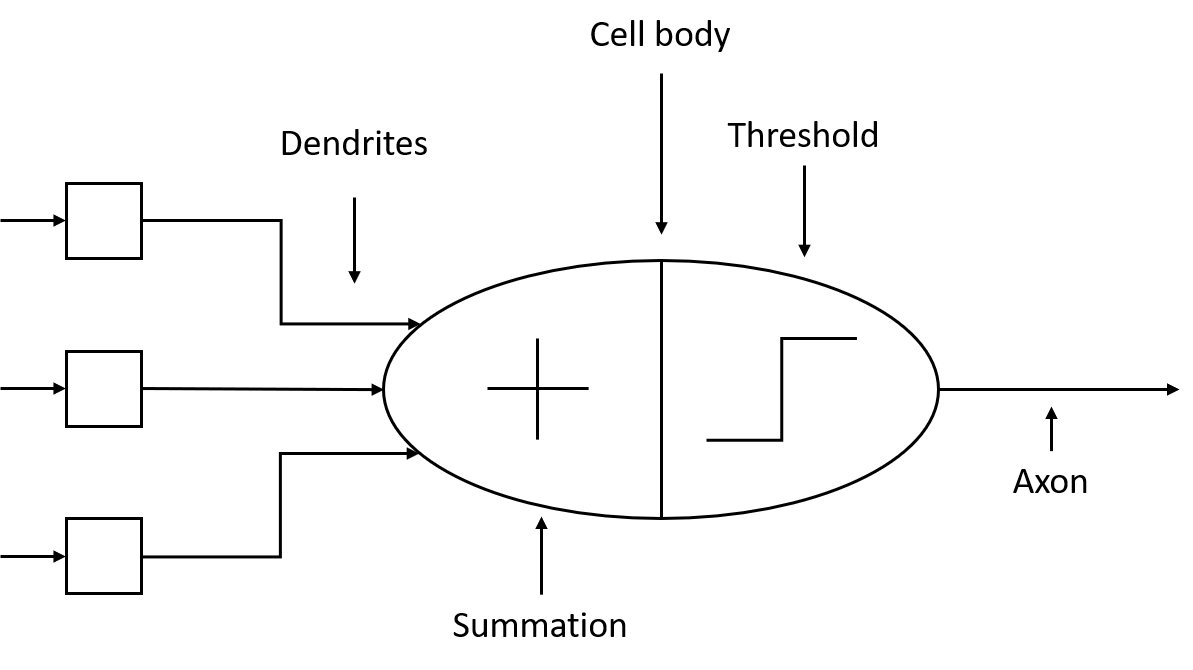
\includegraphics[width=0.5\columnwidth]{chapter01/figure/Picture1.png}
		\centering
	\caption{Hình ảnh minh họa cấu tạo của một nơ-ron sinh học.}
	\label{fig:structureOfNeuron}
\end{figure}

\subsection{Cấu tạo và cách thức hoạt động của một perceptron}
Một nơ-ron nhân tạo (perceptron) được cấu tạo bao gồm các thành phần như hình \ref{fig:structureOfPerceptron}:

\begin{figure}[!h]
	\centering
		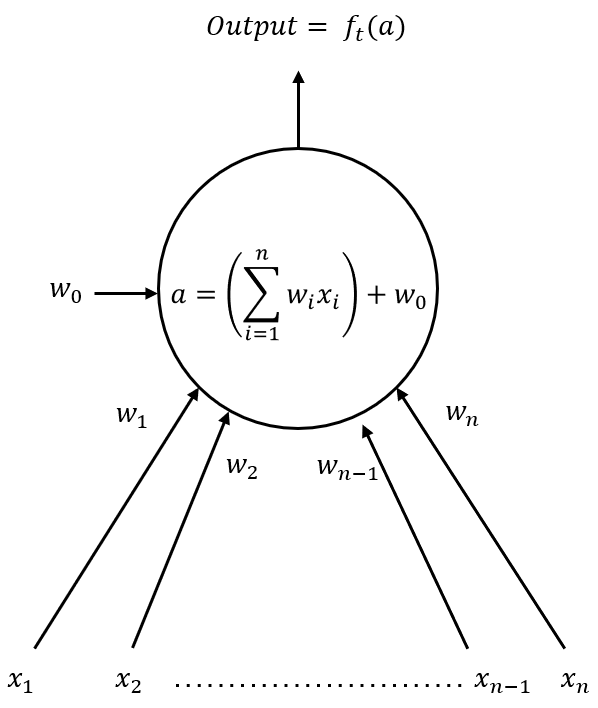
\includegraphics[width=0.4\columnwidth]{chapter01/figure/Picture2.png}
		\centering
	\caption{Hình ảnh minh họa cấu tạo của một perceptron.}
	\label{fig:structureOfPerceptron}
\end{figure}

\noindent Trong đó:
\begin{itemize}
    \item Các giá trị $x_{1},x\textsubscript{2},...,x\textsubscript{n}$ là các tín hiệu đầu vào;
    \item Các giá trị $w\textsubscript{1},w\textsubscript{2},...,w\textsubscript{n}$ là các trọng số của các nhánh tương ứng truyền giá trị $x\textsubscript{1},x\textsubscript{2},...,x\textsubscript{n}$. Giá trị $w\textsubscript{0}$ được gọi là giá trị bias, có thể nhận một giá trị bất kỳ khác 0. Bộ trọng số này là cách để perceptron mô tả độ mạnh yếu của tín hiệu điện trong nơ-ron sinh học;
    \item Giá trị $a$ được tính là $w\textsubscript{0}$ cộng với tổng trọng số của tập tín hiệu đầu vào (tương ứng với bước \textit{summation}). Giá trị a này sẽ được dùng để tính toán hàm kích hoạt $f\textsubscript{t}(a)$;
    \item Kết quả của hàm $f\textsubscript{t}(a)$ sẽ được so sánh với \textit{một ngưỡng (threshsold)} nhằm xác định perceptron có được kích hoạt hay không. Thông thường, giá trị ngưỡng này sẽ được chọn là 0 để tiện trong việc tính toán. Ngoài ra, người ta thường dùng cặp số (1,0) và (1,-1) để đại diện cho trạng thái kích hoạt/không kích hoạt của perceptron;
\end{itemize}
Một điểm lưu ý là perceptron hoạt động dựa trên các phép tính toán số học. Vì vậy, các tín hiệu đầu vào cũng như các trọng số đều cần được biểu diễn dưới dạng các chữ số.

\section{Mạng nơ-ron đa tầng}
\label{sec:MLP}
Có thể thấy rằng, một perceptron đã có thể được coi là một mạng nơ-ron, tính toán kết quả dựa trên tín hiệu đầu vào và kết đầu đầu ra là perceptron đó có được kích hoạt hay không. Trong thực tế, với chỉ một perceptron thì đã có thể giải quyết được bài toán phân loại tuyến tính. Tuy nhiên, đối với các bài toán phức tạp hơn hoặc yêu cầu phân loại phi tuyến (ví dụ như dùng mạng nơ-ron để mô phỏng phép XOR) thì một perceptron không thể đáp ứng được. 
\subsection{Thế nào là mạng nơ-ron đa tầng?}
\label{subsec:whatIsMLP}
Để giải quyết vấn đề trên, chúng ta sử dụng nhiều perceptron được sắp xếp thành các tầng khác nhau. Các perceptron ở tầng sau đều nối tới tầng trước (fully-connected). Một mạng nơ-ron như vậy được gọi là mạng nơ-ron đa tầng.
 
\subsection{Các thành phần của một mạng nơ-ron đa tầng}
\label{subsec:structureOfMLP}
Một mạng nơ-ron đa tầng điển hình thường bao gồm:
\begin{enumerate}
\item Tầng dữ kiện (input layer): Là tầng đầu tiên của mạng,thể hiện các dữ kiện đầu vào;
\item Tầng kết quả (output layer): Là tầng nằm ở vị trí cuối cùng, thể hiện kết quả đầu ra của mạng;
\item Tầng ẩn (hidden layer): Là tầng nằm ở giữa, chịu trách nhiệm trong việc tính toán;
\end{enumerate}

Lưu ý rằng, một mạng nơ-ron đa tầng chỉ có một tầng dữ kiện và một tầng kết quả. Tuy nhiên có thể có một hoặc nhiều tầng ẩn nằm ở giữa, ví dụ như một mạng nơ-ron với hai tầng dưới đây (hình \ref{fig:MLP2HiddenLayer}):

\begin{figure}[h]
	\centering
		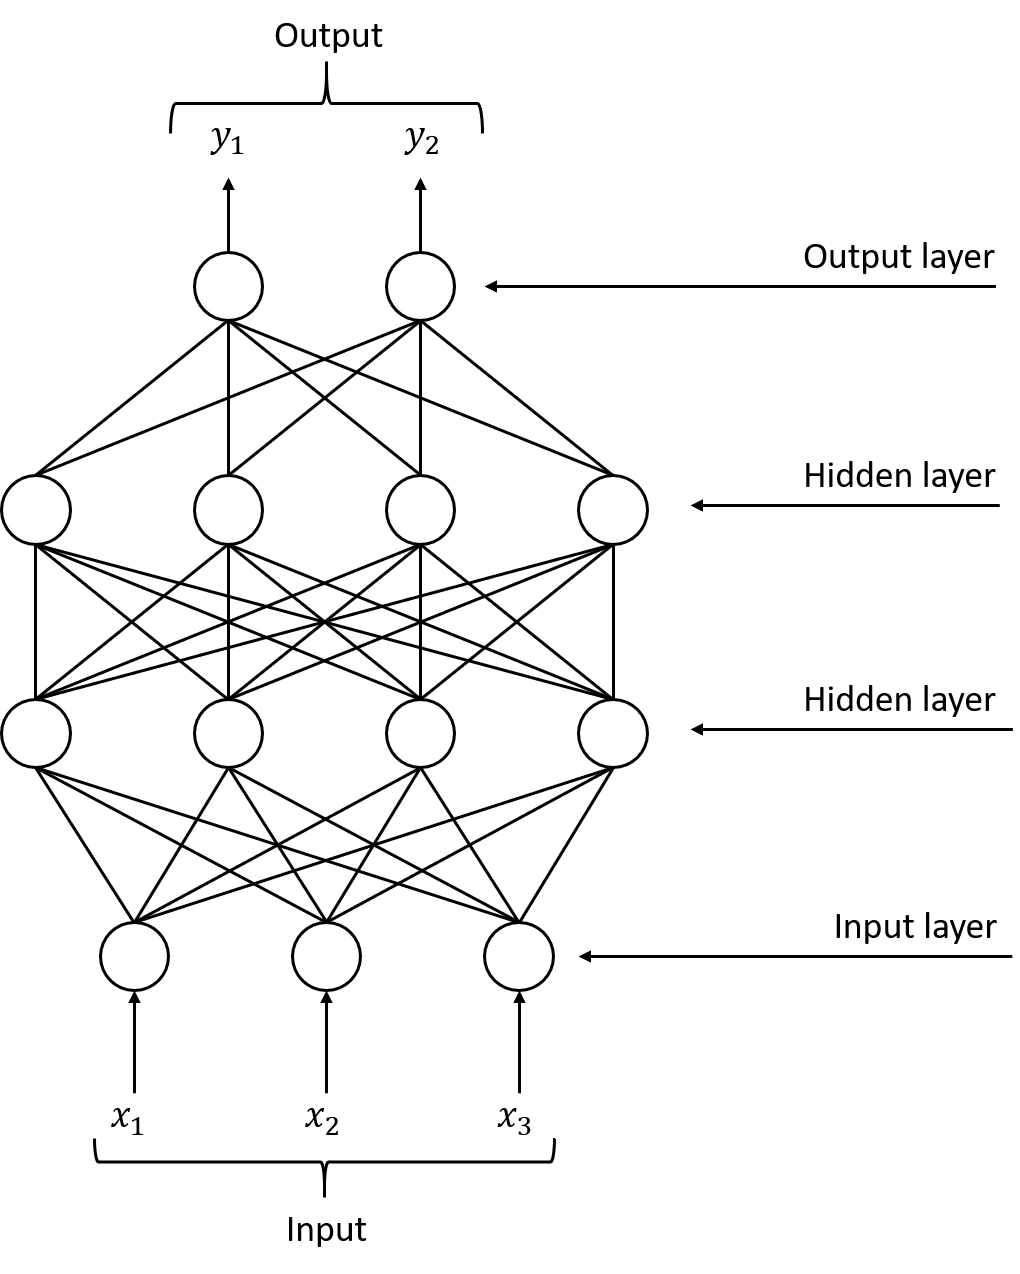
\includegraphics[width=0.5\columnwidth]{chapter01/figure/Picture3.png}
		\centering
	\caption{Hình ảnh mạng nơ-ron đa tầng với 2 tầng ẩn.}
	\label{fig:MLP2HiddenLayer}
\end{figure}

\begin{exmp}
\label{example1}
\hrulefill\\
Cho một mạng nơ-ron ba tầng và các véc-tơ trọng số như hình \ref{fig:example1network} dưới. Với giá trị nào của $x\textsubscript{1}$ và $x\textsubscript{2}$ thì mạng nơ-ron này có kết quả bằng 1?

\begin{figure}[h!]
	\centering
		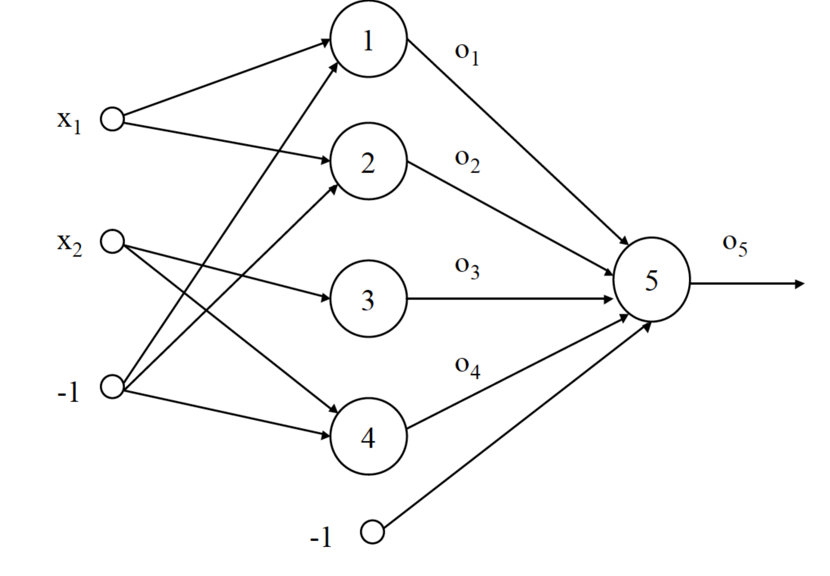
\includegraphics[width=0.7\columnwidth]{chapter01/figure/example 1.png}
		\centering
	\caption{Mạng nơ-ron biểu diễn ví dụ \ref{example1}}
	\label{fig:example1network}
\end{figure}


\noindent Các véc-tơ trọng số có giá trị như sau:

\begin{figure}[h]
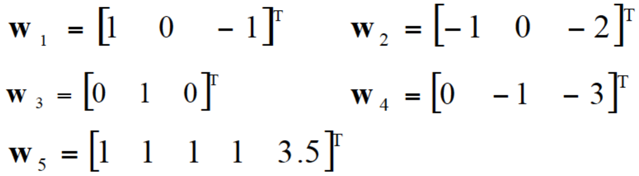
\includegraphics[width=0.6\columnwidth]{chapter01/figure/example 1-weight.png}\
\end{figure}

\noindent Hàm kích hoạt:
\begin{figure}[!h]
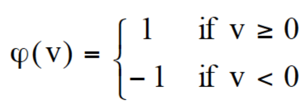
\includegraphics[width=0.3\columnwidth]{chapter01/figure/example 1-activation.png}
\end{figure}

\end{exmp}

\begin{answ}
Chúng ta có thể thấy để thỏa mãn yêu cầu, o\textsubscript{5} phải bằng 1. Điều này dẫn tới nơ-ron số 5 phải được kích hoạt, tương đương với:
\begin{align*} 
&v\textsubscript{5} >= 0 \\ 
\Leftrightarrow &o\textsubscript{1} * 1 + o\textsubscript{2} * 1 + o\textsubscript{3} * 1 + o\textsubscript{4} * 1 + (-1) * 3.5 >= 0
\end{align*}
Như vậy, neural số 1, 2, 3 và 4 phải được kích hoạt để $o\textsubscript{1}, o\textsubscript{2}, o\textsubscript{3}$ và $o\textsubscript{4}$ bằng 1 khiến cho biểu thức trên đúng. Nghĩa là $v\textsubscript{1}, v\textsubscript{2}, v\textsubscript{3}$ và $v\textsubscript{4}$ đều phải lớn hơn hoặc bằng 0. Ta có:
\begin{align}
  &v\textsubscript{1} = x\textsubscript{1} * 1 + x\textsubscript{2} * 0 + (-1) * (-1) = x\textsubscript{1} + 1 \nonumber \\
  \Rightarrow &v\textsubscript{1} >= 0 \Leftrightarrow  x\textsubscript{1} >= -1;  \label{ch1:eq1} \\
  &v\textsubscript{2} = x\textsubscript{1} * (-1) + x\textsubscript{2} * 0 + (-1) * (-2) = -x\textsubscript{1} + 2 \nonumber \\
    \Rightarrow &v\textsubscript{2} >= 0 \Leftrightarrow  x\textsubscript{1} <= 2;  \label{ch1:eq2} \\
  &v\textsubscript{3} = x\textsubscript{1} * 0 + x\textsubscript{2} * (-1) + (-1) * 0 = x\textsubscript{2} \nonumber \\
    \Rightarrow &v\textsubscript{3} >= 0 \Leftrightarrow  x\textsubscript{2} >= 0;  \label{ch1:eq3} \\
  &v\textsubscript{1} = x\textsubscript{1} * 0 + x\textsubscript{2} * (-1) + (-1) * (-3) = -x\textsubscript{2} + 3 \nonumber \\
    \Rightarrow &v\textsubscript{4} >= 0 \Leftrightarrow  x\textsubscript{2} <= 3;  \label{ch1:eq4}
\end{align}
\noindent Từ (\ref{ch1:eq1}), (\ref{ch1:eq2}), (\ref{ch1:eq3}) và (\ref{ch1:eq4}), suy ra để thỏa mãn yêu cầu đã cho thì:
\begin{align*}
-1 <= x\textsubscript{1} <= 2 \And 0 <= x\textsubscript{2} <= 3
\end{align*}
Miền giá trị cần tìm là miền được tô màu đen như hình \ref{fig:example1graph}
\begin{figure}[h]
	\centering
		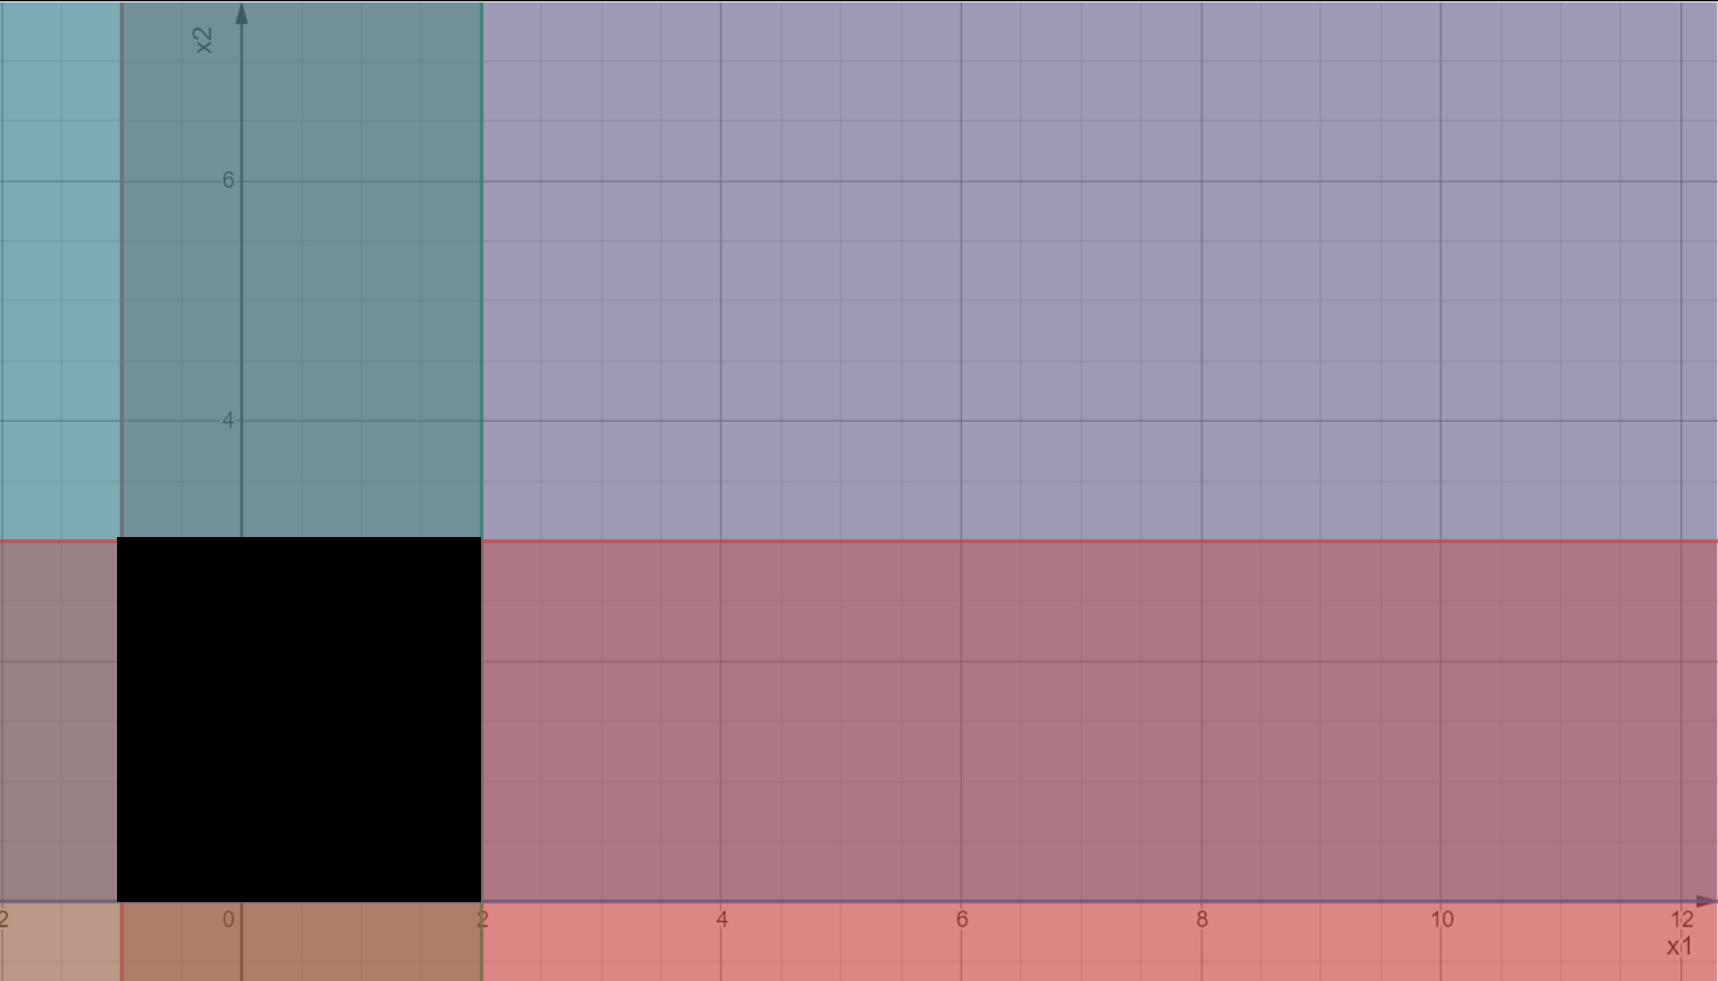
\includegraphics[width=1\columnwidth]{chapter01/figure/example 1_graph.png}
		\centering
	\caption{Miền giá trị cần tìm trong ví dụ \ref{example1}}
	\label{fig:example1graph}
\end{figure}
\end{answ}

\begin{exmp}
\label{example2}
\hrulefill\\
Cho một mạng nơ-ron ba tầng như hình \ref{fig:Example2graph}:

\begin{figure}[h]
	\centering
		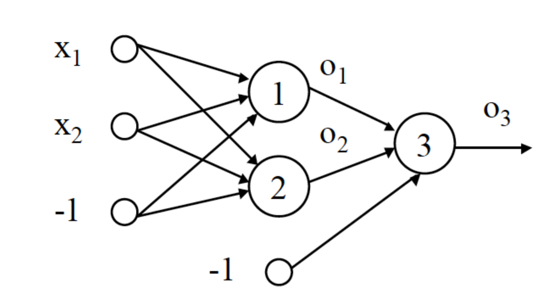
\includegraphics[width=0.7\columnwidth]{chapter01/figure/example 2.png}
		\centering
	\caption{Mạng nơ-ron biểu diễn ví dụ \ref{example2}}
	\label{fig:Example2graph}
\end{figure}

\noindent Các véc-tơ trọng số có giá trị như sau:

\begin{figure}[h]
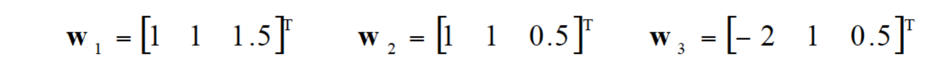
\includegraphics[width=1\columnwidth]{chapter01/figure/example 2-weight .png}
\end{figure}

\noindent Giả sử rằng:

\begin{figure}[!h]
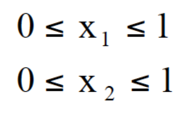
\includegraphics[width=0.2\columnwidth]{chapter01/figure/example 2-assume.png}
\end{figure}

\noindent Với giá trị nào của x\textsubscript{1} và x\textsubscript{2} thì mạng nơ-ron này có kết quả là 1 với hàm kích hoạt như sau:
\begin{figure}[!h]
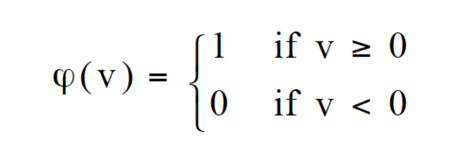
\includegraphics[width=0.4\columnwidth]{chapter01/figure/example 2-activation.png}
\end{figure}
\end{exmp}

\begin{answ}
Tương tự như ví dụ trên, ta có thể thấy rằng:
\begin{align}
  &o\textsubscript{3} = 1 \nonumber \\
  \Leftrightarrow  &o\textsubscript{1} * (-2) + o\textsubscript{2} * 1 + (-1)* 0.5 >= 0 \nonumber \\
  \Leftrightarrow  &-2o\textsubscript{1} + o\textsubscript{2} - 0.5 >= 0 \nonumber
\end{align}
Do o\textsubscript{1} và o\textsubscript{2} chỉ nhận giá trị là 0 hoặc 1. Nên để thỏa mãn biểu thức trên, ta có:
\(o\textsubscript{1} = 0\) và \(o\textsubscript{1} = 1\), trong khi đó:
\begin{align}
  &o\textsubscript{1} = 0 \nonumber\\
  \Leftrightarrow &v\textsubscript{1} = x\textsubscript{1} * 1 + x\textsubscript{2} * 1 + (-1) * 1.5 = x\textsubscript{1} + x\textsubscript{2} - 1.5 < 0 \nonumber\\
  \Rightarrow &x\textsubscript{1} + x\textsubscript{2} < 1.5 \label{eqn:eq2_1}\\
  &o\textsubscript{2} = 1 \nonumber\\
  \Leftrightarrow &v\textsubscript{2} = x\textsubscript{1} * 1 + x\textsubscript{2} * 1 + (-1) * 0.5 = x\textsubscript{1} + x\textsubscript{2} - 0.5 >= 0 \nonumber\\
  \Rightarrow &x\textsubscript{1} + x\textsubscript{2} >= 0.5 \label{eqn:eq2_2}
\end{align}
\noindent Từ \ref{eqn:eq2_1} và \ref{eqn:eq2_2} suy ra kết quả cần tìm: \( 0.5 <= x\textsubscript{1} + x\textsubscript{2} < 1.5\)\\

\noindent Như vậy, kết quả cần tìm là cặp giá trị x\textsubscript{1} và x\textsubscript{2} sao cho điều kiện trên thỏa mãn. Một điểm đặc biệt là nếu như x\textsubscript{1} và x\textsubscript{2} chỉ nhận giá trị 0 và 1 thì mạng nơ-ron này có thể áp dụng để biểu diễn phép toán luận lý XOR (tham khảo Bảng dự thật dưới đây).

\begin{figure}[h]
	\centering
		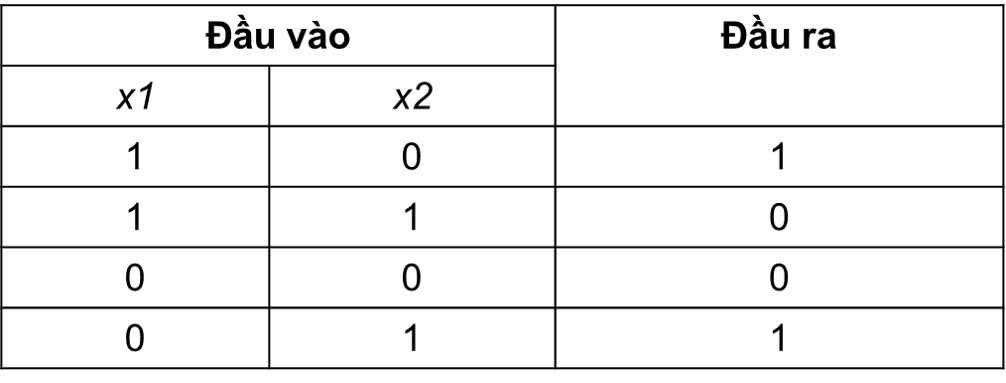
\includegraphics[width=0.6\columnwidth]{chapter01/figure/bang su that XOR.png}
		\centering
	\caption{Bảng sự thật biểu diễn phép XOR trong ví dụ \ref{example2}}
\end{figure}
\end{answ}

\section{Sử dụng neural network cho bài toán phân loại}
\label{sec:classification}
Một trong những ứng dụng quan trọng của mạng nơ-ron là sử dụng cho bài toán phân loại. Đối với bài toán phân loại tuyến tính thì chỉ cần xây dựng mạng nơ-ron với một perceptron. Xét ví dụ sau:

\begin{exmp}
\label{example3}
\hrulefill\\
Xem xét bài toán trong thực tế như sau: Một trường chuyên tổ chức thi để tuyển sinh năm học mới, bao gồm hai môn Toán và Văn, trong đó Toán nhân hệ số 2. Để có thể đậu, học sinh cần phải có tổng điểm xét tuyển lớn hơn hoặc bằng 21. 

Hãy xây dựng một mạng nơ-ron để phân loại học sinh, trong đó điểm Toán được ký hiệu là x, điểm Văn được ký hiệu là y. Kết quả của mạng là 0 hoặc 1, tương đương với học sinh đó đậu hoặc rớt.
\end{exmp}
\begin{answ}
Theo yêu cầu bài toán, ta cần xây dựng mạng nơ-ron dựa trên biểu thức sau:
\begin{align*}
  &2x + y >= 21 \\
  \Leftrightarrow &2x + y -21 >= 0
\end{align*}
Như vậy, khi chuyển sang biểu diễn dưới dạng một mạng nơ-ron, ta có tập giá trị đầu vào là một véc-tơ [x,y,1] và tập trọng số tương ứng có giá trị là [2,1,-21], với \(w\textsubscript{0} = -21\) (trọng số bias tùy ý khác 0). 

\begin{figure}[h]
	\centering
		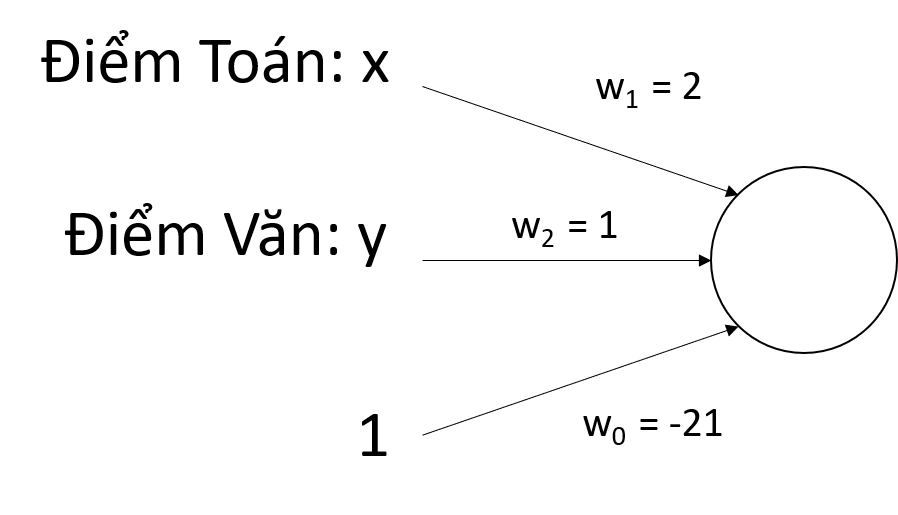
\includegraphics[width=0.5\columnwidth]{chapter01/figure/example 3.png}
        \caption{Mạng nơ-ron biểu diễn ví dụ \ref{example3}}
		\centering
\end{figure}

Ta có, tổng trọng số \(a = 2x + y - 21\). Mạng nơ-ron này chỉ được kích hoạt (tương đương với học sinh đó thỏa mãn điều kiện đậu) khi và chỉ khi \(a >= 0\), tương ứng với vùng màu xanh dương trong biểu đồ \ref{fig:example3-miengiatri}.

\begin{figure}[!h]
	\centering
		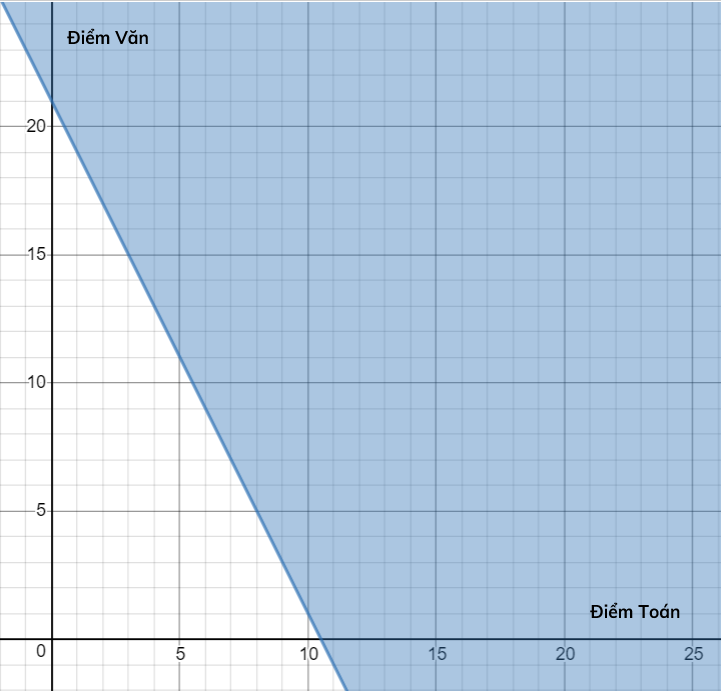
\includegraphics[width=0.55\columnwidth]{chapter01/figure/example 3 - graph 1.PNG}
        \caption{Miền giá trị thỏa mãn yêu cầu đề bài}
        \label{fig:example3-miengiatri}
		\centering
\end{figure}

Tuy nhiên, thực tế điểm Toán và điểm Văn luôn nhận giá trị là số dương \(<= 10\). Khi gán thêm điều kiện này, ta có kết quả là miền giá trị được tô màu đen trong đồ thị \ref{fig:example3-miengiatri2}.

\begin{figure}[h!]
	\centering
		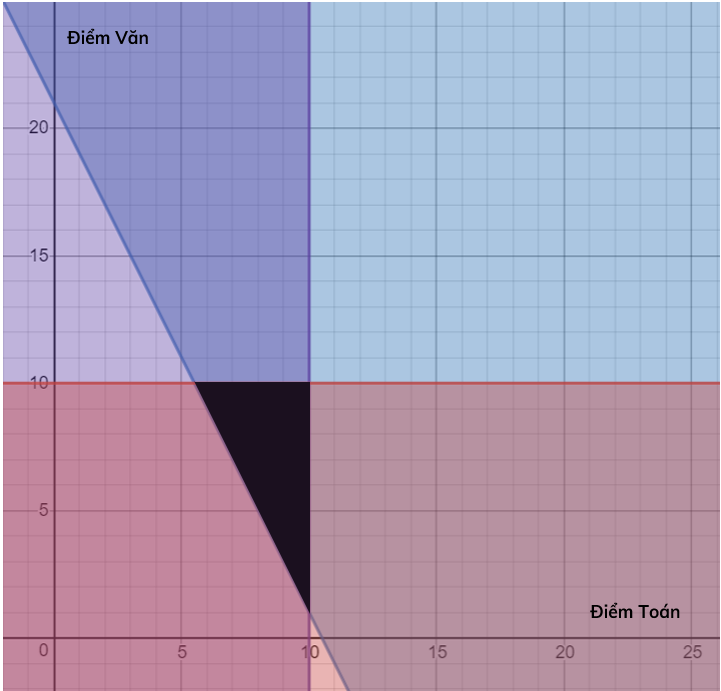
\includegraphics[width=0.55\columnwidth]{chapter01/figure/example 3 - graph 2.PNG}
        \caption{Miền giá trị thỏa mãn yêu cầu đề bài sau khi ràng buộc về khoảng giá trị của điểm Toán và điểm Văn}
        \label{fig:example3-miengiatri2}
		\centering
\end{figure}

Cần lưu ý rằng trọng số bias phải khác 0 để tránh trường hợp phương trình tổng trọng số a được biểu diễn bởi một đường thẳng đi qua gốc tọa độ O(0,0). Điều này dẫn tới khi huấn luyện mạng nơ-ron, thì các kết quả mà mạng này học được chỉ xoay quanh gốc tọa độ O, không đảm bảo tính tổng quát để áp dụng cho các bài toán trong thực tiễn.
\end{answ}
Ví dụ trên đã sử dụng mạng nơ-ron với một perceptron để phân loại bài toán tuyến tính (như hình \ref{fig:neuronRegion}.a bên dưới). Tuy nhiên, đối với bài toán phi tuyến (như các hình \ref{fig:neuronRegion}.b, c, d) thì cần phải xây dựng mạng nơ-ron ba tầng.

\begin{figure}[!h]
	\centering
		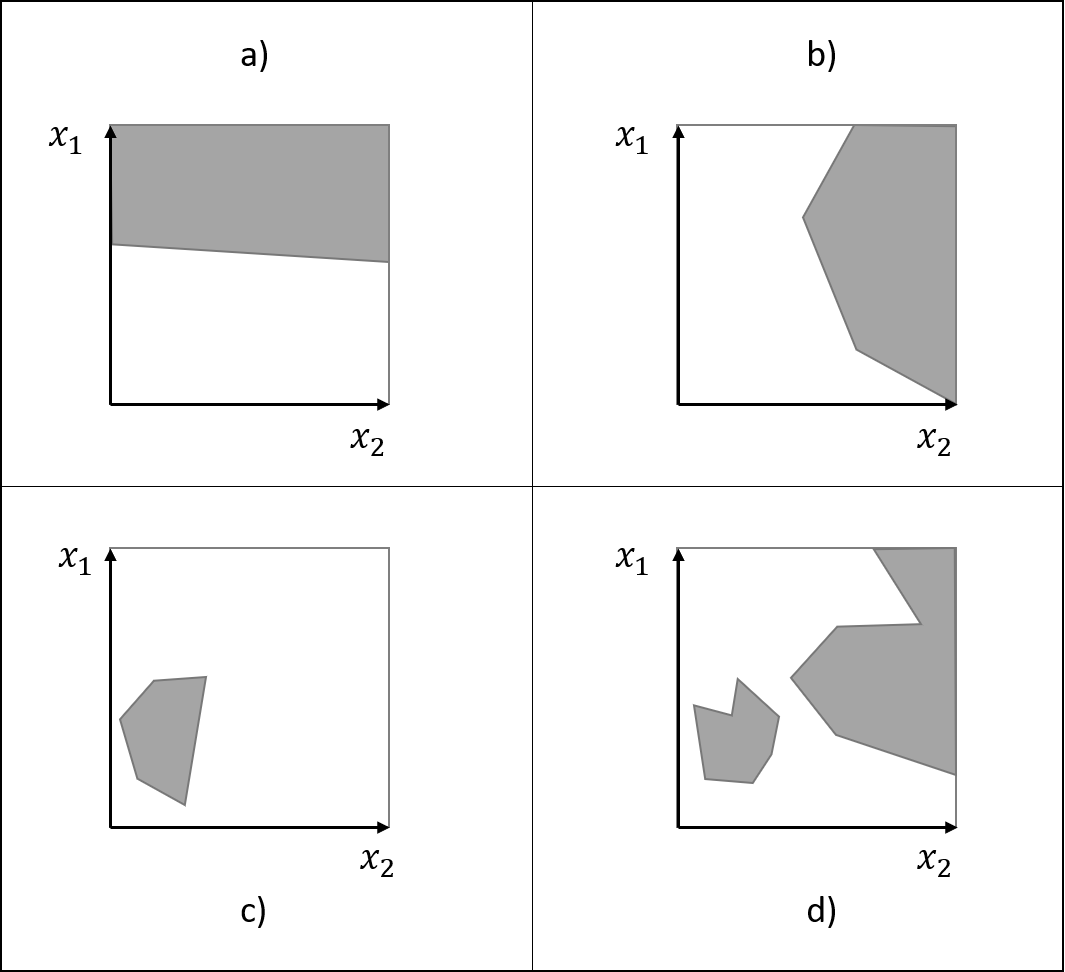
\includegraphics[width=0.6\columnwidth]{chapter01/figure/Picture4.png}
    	\caption{Sử dụng mạng nơ-ron ba tầng để biểu diễn các miền giá trị phi tuyến}
	\centering
	\label{fig:neuronRegion}
\end{figure}

Trong đó, tầng đầu tiên (tầng dữ kiện) sẽ chia đồ thị thành hai nửa bởi một đường thẳng. Tầng thứ hai (tầng ẩn) sẽ hình thành các miền giá trị cần tìm bằng cách kết hợp các phép toán luận lý (AND, OR và NOT) trên nửa đồ thị đã được phân chia của tầng đầu tiên. Bằng cách tăng số lượng tầng ẩn, mạng nơ-ron thậm chí có thể biểu diễn gần đúng các hình tròn thông qua một tập các đường thẳng, ví dụ như hình \ref{fig:circleNeuron}

\begin{figure}[!h]
	\centering
		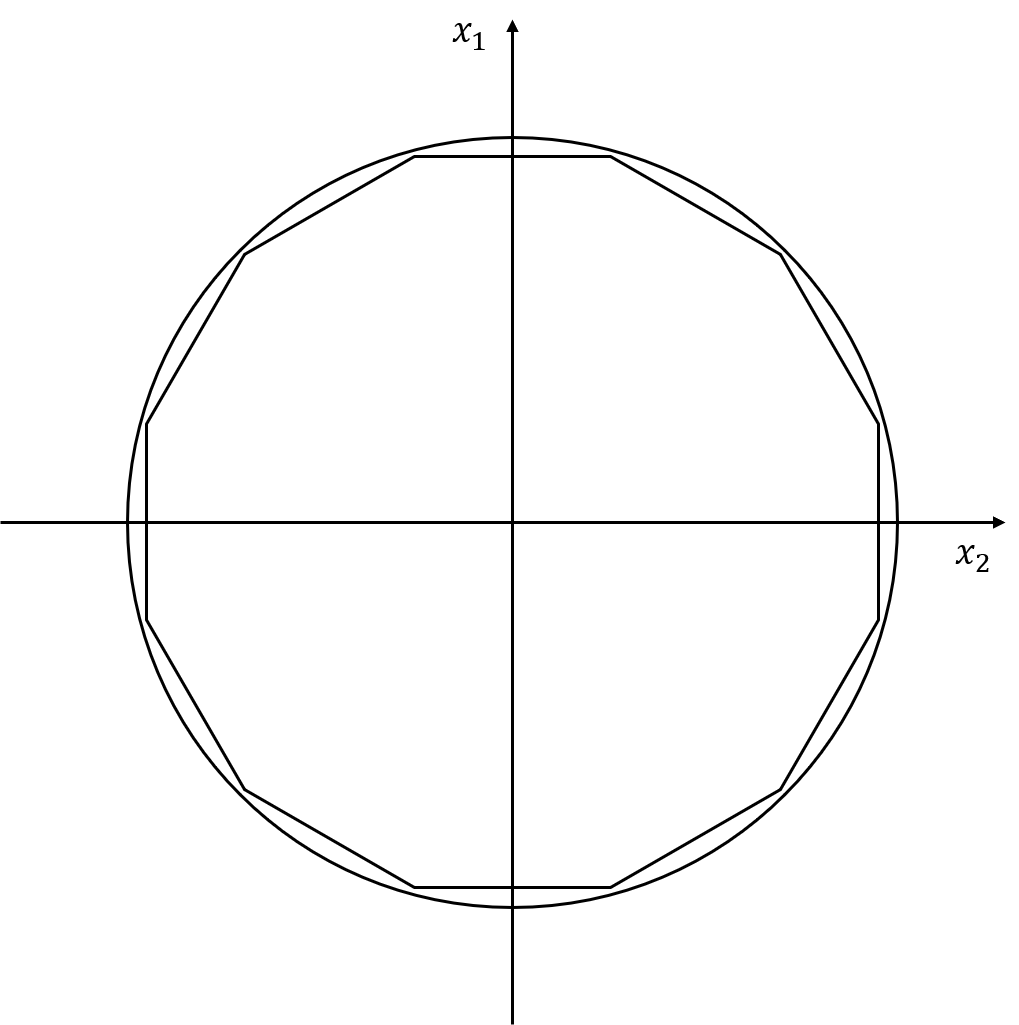
\includegraphics[width=0.5\columnwidth]{chapter01/figure/Picture5.png}
    	\caption{Sử dụng mạng nơ-ron để biển diễn gần đúng miền giá trị là hình tròn}
	\centering
	\label{fig:circleNeuron}
\end{figure}

\section{Kết chương}
\label{sec:endChp}

Chúng ta có thể thấy rằng, mạng nơ-ron được biểu diễn toàn bộ bằng các phép toán số học. Vì vậy, nếu tìm được các bộ trọng số phù hợp với từng bài toán phân loại thì ta hoàn toàn có thể áp dụng mạng nơ-ron một cách hiệu quả, nhanh chóng bằng cách cấu hình sẵn phần cứng với các trọng số cần thiết. 

Tuy nhiên, trong thực tế thì việc để tìm được các bộ trọng số không dễ dàng, đặc biệt là đối với những bài toán phức tạp và cần mô hình bởi mạng nơ-ron đa tầng với nhiều tầng ẩn và nhiều perceptron. Để giải quyết vấn đề này, các nhà khoa học đã tìm ra được phương pháp huấn luyện mạng nơ-ron để có thể tìm ra bộ trọng số tối ưu, vấn đề này sẽ được trình bày trong chương tiếp theo.

\newpage

\section{Bài tập}

\begin{exer}
\label{chp01:exer1}
Cho một mạng nơ-ron ba tầng và các véc-tơ trọng số như hình \ref{fig:exercise1}. Với giá trị nào của x\textsubscript{1} và x\textsubscript{2} thì mạng nơ-ron này có kết quả bằng 1? Vẽ biểu đồ minh họa.
\begin{figure}[!h]
	\centering
		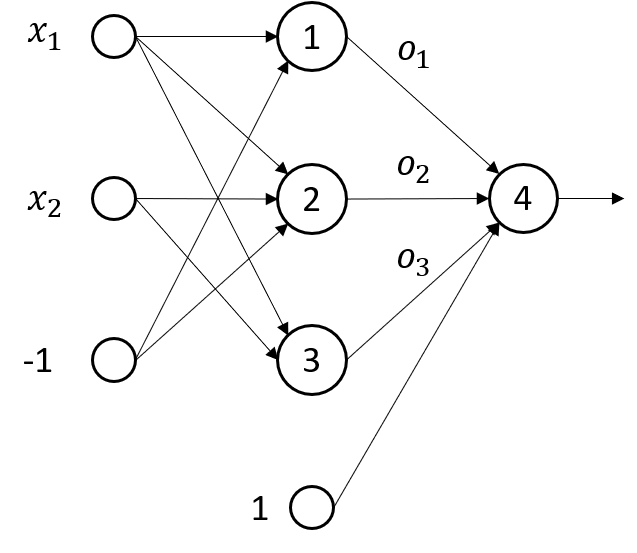
\includegraphics[width=0.5\columnwidth]{chapter01/figure/excercise-1.png}
    	\caption{Mạng nơ-ron trong bài tập \ref{chp01:exer1}}
	\centering
	\label{fig:exercise1}
\end{figure}

Các véc-tơ trọng số có giá trị như sau:
\begin{align*}
w\textsubscript{1} = [2,0,1] \textsuperscript{T} \quad w\textsubscript{2} = [1,2,1] \textsuperscript{T} \quad w\textsubscript{3} = [1,3,0] \textsuperscript{T} \quad w\textsubscript{4} = [2,3,1] \textsuperscript{T} \quad
\end{align*}

Hàm kích hoạt
\begin{align*}
        \varphi (v) = \left\{ \begin{array}{ll}
        1 & \mbox{nếu $v \geq 0$};\\
        0 & \mbox{nếu $v < 0$}.\end{array} \right.
\end{align*}
\end{exer}

\begin{exer}
\label{chp01:exer2}
Thiết kế một mạng nơ-ron để chọn ra các sinh viên toàn diện. Tiêu chí để chọn bao gồm điểm trung bình (số nguyên dương), hạnh kiểm (bao gồm các mức 0-Yếu, 1-Trung Bình, 2-Khá, 3-Giỏi) và điểm rèn luyện (thấp nhất là 0 điểm và cao nhất là 10 điểm). Xét biểu thức sau:\\
\\
\textit{Điểm danh hiệu =  điểm trung bình x 2 + điểm hạnh kiểm + điểm rèn luyện;}\\
\\
\noindent Sinh viên sẽ được nhận danh hiệu toàn diện nếu như \textit{điểm danh hiệu} lớn hơn hoặc bằng 24.
\end{exer}

\begin{exer}
Trong bài tập \ref{chp01:exer2}, nếu như thay đổi  bias đã chọn ban đầu thành một giá trị khác (tùy chọn), thì tập trọng số sẽ cần thay đổi như thế nào?
\end{exer}

\begin{exer}
Trong bài tập \ref{chp01:exer1}, nếu như thay đổi giá trị bias ở tầng thứ 2 từ 1 sang -1. Thì miền giá trị x\textsubscript{1} và x\textsubscript{2} cần tìm có thay đổi không? Vẽ lại biểu đồ minh họa cho trường hợp này và so sánh với trường hợp ban đầu.
\end{exer}
\chapter{Logistic Regression}
\label{chp:02}

\section{Giới thiệu về Logistic Regression}
\textit{Logistic Regression} là mô hình được đặt tên dựa trên hàm số mà nó đóng vai trò cốt lõi của mô hình, đó là hàm \textit{logistic}. Hàm \textit{logistic} được tạo ra ra bởi những nhà thống kê để đặc tả sự bùng nổ dân số. Hàm \textit{logistic} có dạng hình chữ S có thể nhận đầu vào là số thực và có miền giá trị là $(0, L)$. Biểu thức toán học tổng quát của hàm \textit{logistic}:
%\begin{equation*}
  %f(x)=\frac{L}{1 + e^{-k(x-x_{0})}}  
%\end{equation*}
\begin{align*}
f(x)=\frac{L}{1 + e^{-k(x-x_{0})}}, \text{ với} \quad &x_{0} \text{ là giá trị chính giữa của đường cong logistic.}\\
     &k \text{ là tỷ lệ tăng của hàm logistic.}\\
    &L \text{ là giá trị cực đại của hàm logistic.}
\end{align*}

Mô hình \textit{Logistic Regression} giống \textit{Linear Regression} ở khía cạnh sử dụng biểu thức toán học để biển diễn, và giống với \textit{Perception Learning Algorithm} ở việc đầu ra bị chặn. Tuy nhiên, \textit{Logistic Regression} thường được sử dụng nhiều hơn cho các bài toán phân loại mặc dù trong tên có chứa từ $"Regression"$. Trong phần tiếp theo sẽ làm rõ tại sao \textit{Logistic Regression} lại thích hợp với bài toán phân loại, đặc biệt là phân loại nhị phân.

\section{Bài toán Supervised learning và hàm Sigmoid activation}
Cũng giống như \textit{Linear Regression}, \textit{Logistic Regression} được sử dụng để giải bài toán \textit{Supervised Learning}. Tuy nhiên, \textit{Logistic Regression} được dùng để giải các bài toán phân loại, còn \textit{Linear Regression} được dùng để dự đoán cho các bài toán có giá trị liên tục (như dự đoán giá nhà). Câu hỏi đặt ra là tại sao không dùng \textit{Linear Regression} thay vì \textit{Logistic Regression} để giải bài toán phân loại. Chúng ta sẽ lấy ví dụ để minh chứng sự vượt trội của \textit{Logistic Regression} so với \textit{Linear Regression} khi áp dụng vào bài toán phân loại, cụ thể là phân loại nhị phân.
\\
\begin{exmp}
\label{exmp:o}
\hrulefill\\
%%%
Một nhóm 20 người có chiều cao từ 1.4 m đến 1.8 m. Từ chiều cao của mỗi người chúng ta sẽ dự đoán xem họ là nam (M) hay nữ (F).\\
\\
Ta có tập dữ liệu như bảng \ref{Tab:ex}:\\
\begin{table*}[ht]
\centering
\begin{tabular}{|l|l|l|l|}
\hline
Height & Gender \\ \hline
1.5   & F \\ \hline
1.75  & M \\ \hline
1.6     & M \\ \hline
1.45  & F  \\ \hline
1.55   & F \\ \hline
1.7  & M \\ \hline
1.65  & M \\ \hline
1.4     & F \\ \hline
1.8  & M \\ \hline
1.6.5   & M \\ \hline
1.65  & F \\ \hline
1.55   & M \\ \hline
1.6  & F \\ \hline
1.5   & M \\ \hline
\end{tabular}
\caption{Dữ liệu đầu vào của ví dụ \ref{exmp:o}}
\label{Tab:ex}
\end{table*}
\end{exmp}

Để trực quan hơn, ta biểu diễn dữ liệu trên tọa độ không gian 2 chiều ở hình \ref{fig:sec2ex1}:
\begin{figure}[!ht]
    \centering
    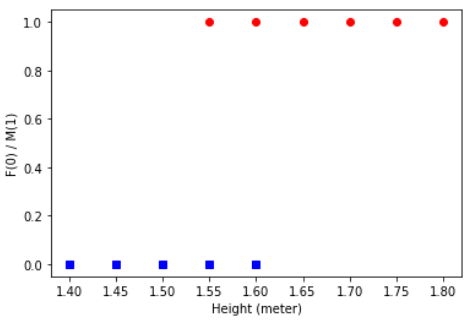
\includegraphics[scale=0.5]{chapter02/figure/example1.png}
    \caption{Đồ thị các điểm dữ liệu.}
    \label{fig:sec2ex1}
\end{figure}

Trong ví dụ này, đầu vào của mô hình là vector $\mathbf{X}$ tương ứng với chiều cao của nhóm người và đầu ra là vector $\mathbf{y}$ tương ứng với giới tính của họ (M/F). Ta khởi tạo vector trọng số $\mathbf{W}$ có chiều dài bằng với vector $\mathbf{X}$ và biến $\mathbf{b}$ (bias). Gọi $\mathbf{\hat{y}}$ là xác suất một người là nam khi biết chiều cao của người đó là ($\hat{y}$ $=$ $P(y=1|x)$) và $\mathbf{\hat{y}}$ nằm trong khoảng $[0, 1]$.

%Tiếp theo, ta làm rõ tại sao \textit{Linear Regression} không phù hợp với bài toán phân loại.\\

Trong mô hình \textit{Linear Regression}, ta có đầu ra dự đoán là:
\begin{equation*}
    \hat{y} = z = W^TX + b
\end{equation*}

Khi áp dụng \textit{Linear Regression} vào bài toán trên chúng ta có thể thu được kết quả như hình \ref{fig:lr_result}:
\clearpage
\begin{figure}[!ht]
    \centering
    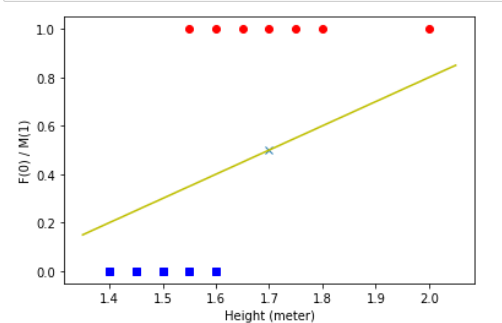
\includegraphics[width=\textwidth,height=\textheight,keepaspectratio]{chapter02/figure/LN_result.PNG}
    \caption{Kết quả khi dùng Linear Regression.}
    \label{fig:lr_result}
\end{figure}

Trong hình \ref{fig:lr_result}, đường màu vàng biểu diễn đường \textit{Linear Regression}. Có hai vấn đề có thể thấy được từ kết quả của \textit{Linear Regression}:

\begin{itemize}
    \item Đường thẳng \textit{Linear Regression} không bị chặn nên nó thể cho ra kết quả không nằm trong vùng mong muốn như trên hình trên đường thẳng có thể cho ra giá trị $\mathbf{\hat{y}}$ > 1 và $\mathbf{\hat{y}}$ < 0 nên mô hình này không phù hợp cho bài toán này. Tuy nhiên, chúng ta có thể chặn đường thẳng trên bằng cách cắt phần nhỏ hơn 0 bằng cách cho chúng bằng 0, cắt các phần lớn hơn 1 bằng cách cho chúng bằng 1.
    \item \textit{Linear Regression} không có khả năng phân loại tốt với dự liệu bị mất cân bằng. Nếu chúng ta lấy điểm trên đường thẳng này có tung độ bằng 0.5 là điểm ngưỡng phân chia hai lớp (là nam nếu $\mathbf{\hat{y}}$ $> 0.5$, ngược lại là nữ). Giả sử có thêm một người có chiều cao 1.9 mét và là nam. Khi áp dụng mô hình \textit{Linear Regression}, đường thẳng sẽ bị lệch về bên phải (như hình \ref{fig:lr_result}) sẽ dẫn đến hiện tượng toàn bộ những người nữ vẫn được dự đoán là nữ, nhưng những người là nam nhưng được dự đoán là nữ.
\end{itemize}

Vì vậy chúng ta cần một mô hình khác thể cho ta đường phân chia tốt hơn so với \textit{Linear Regression} và thỏa mãn các tính sau:

\begin{itemize}
    \itemsep0em 
    \item Là hàm số nhận giá trị thực, bị chặn trong khoảng (0,1).
    \item Nếu coi điểm có tung độ là $0.5$ làm điểm phân chia thì các điểm càng xa điểm này về phía bên trái có giá trị càng gần $0$. Ngược lại, các điểm càng xa điểm này về phía phải có giá trị càng gần 1. Điều này khớp với nhận xét rằng học càng nhiều thì xác suất đỗ càng cao và ngược lại.
    \item Hàm liên tục để có thể đạo hàm mọi nơi, để giúp tìm điểm tối ưu khi sử dụng \textit{Gradient Descent}.
\end{itemize}

Ta thấy, Hàm \textit{Sigmoid} (là hàm \textit{Logistic} với $L = 1$, $k = 1$ và $x_{0} = 0$) thỏa mãn 3 tính chất nói trên. Phương trình của hàm \textit{Sigmoid}:

\begin{equation}
    f(z)= \sigma(z) = \frac{1}{1 + e^{-z}}
    \label{eq:esigmoid}
\end{equation}

Đồ thị của hàm \textit{Sigmoid}:
\begin{figure}[!ht]
    \centering
    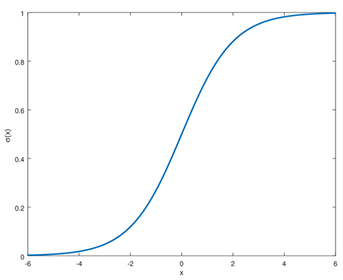
\includegraphics[scale=0.8]{chapter02/figure/sigmoid.png}
    \caption{Đồ thị các điểm dữ liệu.}
    \label{fig:sigmoid}
\end{figure}

Từ phương trình (\ref{eq:esigmoid}) và đồ thị hình \ref{fig:sigmoid}, ta có thể dễ dàng thấy \newline $\lim_{s \rightarrow -\infty}\sigma(s) = 0$ và $\lim_{s \rightarrow +\infty}\sigma(s) = 1$. Vì vậy miền giá trị của hàm \textit{Sigmoid} luôn là $(0, 1)$, rất thích hợp với việc phân loại nhị phân. Ngoài ra, khi đầu vào  rất lớn (hoặc rất nhỏ) thì giá trị đầu ra của hàm \textit{Sigmoid} luôn tiến tới tiệm cận 1 hoặc 0, nên hàm \textit{Sigmoid} có thể xử lý việc dữ liệu bị mất cân bằng, là vấn đề đã nêu trên của \textit{Linear Regression}. Áp dụng hàm \textit{Sigmoid} vào ví dụ \ref{exmp:o}, ta lấy $\mathbf{W^TX + b}$ làm dữ liệu đầu vào của hàm \textit{Sigmoid}. Phương trình mới của kết quả dự đoán $\hat{y}$:
\begin{align*}
    \hat{y}= \sigma(z) = \sigma(W^TX + b)
\end{align*}
     
%\end{equation*}
Với ngưỡng phân loại là 0.5, như  kết quả thu được ở hình \ref{fig:lg_result}: ta có thể thấy, \textit{Logistic Regression} có khả năng phân loại tốt hơn nhiều so với \textit{Linear Regression},

\begin{figure}[!ht]
    \centering
    %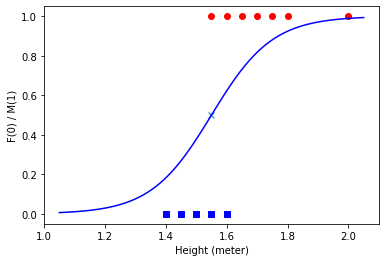
\includegraphics[width=\textwidth,height=\textheight,keepaspectratio]{chapter02/figure/LG_result.png}
    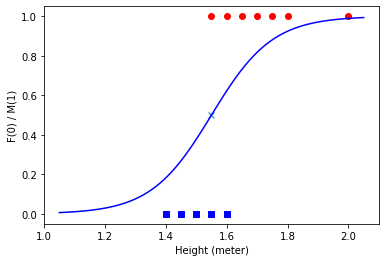
\includegraphics[scale=0.8]{chapter02/figure/LG_result.png}
    \caption{Kết quả khi dùng Logistic Regression.}
    \label{fig:lg_result}
\end{figure}

\section{Hàm Cost function của Logistic Regression}
Trước khi đi vào nội dung chính của phần này, chúng ta sẽ tìm hiểu về khái niệm hàm lồi (convex function) và hàm không lồi (non-convex function):

\begin{itemize}
    \item Hàm $f$ được gọi là lồi trên đoạn $[\alpha, \beta] \subset R$ nếu với mọi $x,y \in [\alpha, \beta]$ và với mọi $a, b \geq 0$ thỏa $a + b = 1$ thì: $f(ax + by) \geq af(x) + bf(y)$. Nếu $f$ là hàm lồi trên $[\alpha, \beta]$ thì ta có: $min(f)=min{f(\alpha), f(\beta)}$ nên hàm lồi chỉ có 1 điểm cực tiểu và đó là điểm mà hàm có giá trị nhỏ nhất trên miền giá trị của nó (global minimum).
    \item Hàm $f$ được gọi là hàm không lồi khi nó không có tính chất lồi. Đồ thị hàm không lồi thường có dạng sóng với nhiều điểm cực trị (cực tiểu hoặc cực đại) (local optimal). 
\end{itemize}

\begin{figure}[!htb] 
   \begin{minipage}{0.48\textwidth}
     \centering
     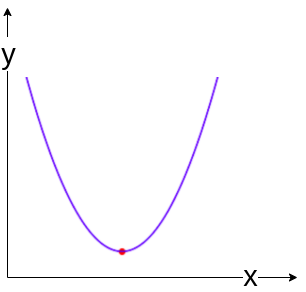
\includegraphics[width=1\linewidth]{chapter02/figure/convex.png}
   \end{minipage}\hfill
   \begin{minipage}{0.48\textwidth}
     \centering
     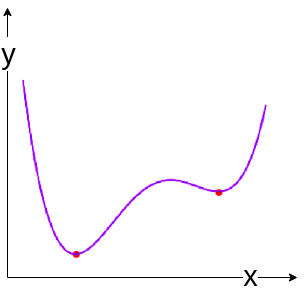
\includegraphics[width=1\linewidth]{chapter02/figure/non_convex.png}
   \end{minipage}
   \caption{Đồ thị hàm convex (bên trái) và đồ thị hàm non-convex (bên phải)}
   \label{fig:convex}
\end{figure}

Tiếp theo ta sẽ đi vào nội dung chính của phần này. Nhắc lại, trong mô hình \textit{Logistic Regression}, ta có:
\begin{equation*}
    \hat{y}= \sigma(z) = \sigma(W^TX + b) 
\end{equation*}

Cũng như phương pháp giải các bài toán \textit{Supervised Learning}, quá trình học của mô hình \textit{Logistic Regression} là quá trình cập nhật trọng số $\mathbf{W}$ vì vậy \textit{Logistic Regression} cũng cần có một hàm mất mát (Loss Function) để đánh giá sự sai biệt giữa kết quả dự đoán $\hat{y}$ và kết quả thực tế $y$. Ta ký hiệu $\mathcal{L}(\hat{y}, y)$ là hàm mất mát.

Hàm mất mát đơn giản nhất chính là \textit{Least Squared Error (LSE)} có phương trình là: 
\begin{equation*}
    \mathcal{L}(\hat{y}, y) = \frac{1}{2}(\hat{y} - y)^2
\end{equation*}

%Vì phương trình kết quả dự đoán của \textit{Linear Regression} là $\hat{y} =  w^TX + b$ nên hàm LSE là hàm lồi và chúng ta có thể đạt được điểm tối ưu của hàm với giá trị mất mát nhỏ nhất (hình 1.5 bên trái).
Tuy nhiên, đối với \textit{Logistic Regression}, chúng ta không dùng LSE làm hàm mất mát bởi vì phương trình kết quả dự đoán của \textit{Logistic Regression} $\hat{y} = \sigma(w^TX + b)$ nên khi đó LSE là một hàm không lồi với nhiều điểm cực tiểu (hình \ref{fig:convex} bên phải).

LSE không đảm bảo tìm được điểm tối ưu toàn cục khi giải bài toán \textit{Logistic Regression}. Vì vậy, chúng ta cần có một hàm mất mát khác cho \textit{Logistic Regression} và đó là hàm \textit{Cross-Entropy}. Phương trình hàm mất mát khi đó:
\begin{equation} \label{eq:ce}
    \mathcal{L}(\hat{y}, y) = -(y\log_{}{\hat{y}} + (1 - y)\log_{}{(1 - \hat{y})})
\end{equation}

Vì tập giá trị của $y$ là $\{0,1\}$ nên từ phương trình \eqref{eq:ce}, ta có thể thấy:
\begin{itemize}
    \item Khi $y = 0$: phương trình \eqref{eq:ce} sẽ trở thành $L(\hat{y}, y) = -\log_{}{(1 - \hat{y})}$. Trong trường hợp này, nếu kết quả dự đoán $\hat{y}$ của chúng ta càng gần về giá trị $0$ thì hàm mất mát cho ra giá trị càng nhỏ và ngược lại, đáp ứng đúng như yêu cầu chúng ta mong muốn.
    \item  Khi $y = 1$: phương trình \eqref{eq:ce} sẽ trở thành $L(\hat{y}, y) = -\log_{}{(\hat{y})}$. Trong trường hợp này, nếu kết quả dự đoán $\hat{y}$ của chúng ta càng gần về giá trị $1$ thì hàm mất mát cho ra giá trị càng nhỏ và ngược lại, đáp ứng đúng như yêu cầu chúng ta mong muốn.
    \item Với việc $\hat{y}$ bằng các giá trị đầu mút ($0$ và $1$) khi và chỉ khi đầu vào của hàm sigmoid là vô cùng, điều không xảy ra với các phép toán tự nhiên nên ta có thể thấy hàm mất mát luôn cho giá trị có ý nghĩa.
\end{itemize}

Tiếp theo, chúng ta sẽ giải thích tại sao \textit{Cross-Entropy} có thể giúp mô hình \textit{Logistic Regression} tìm được điểm tối ưu toàn cục. Để dễ dàng chứng minh ta viết lại phương trình của kết quả dự đoán $\hat{y}$ như sau:
\begin{equation*}
    \hat{y} = \theta^TX
\end{equation*}
\begin{align*}
  \text{với} \quad &X \text{ là ma trận đầu vào có thêm một cột vector có giá trị của các hàng }\\
  & \text{đều bằng 1 (giá trị của bias)}\\
     &\theta \text{ là các trọng số của mô hình Logistic Regression.}
\end{align*}
Từ phương trình \eqref{eq:ce}, ta có:
%\begin{equation*}
\begin{align}
-\mathcal{L}(\hat{y}, y) & = y\log_{}{\hat{y}} + (1 - y)\log_{}{(1 - \hat{y})} \nonumber\\
              & = y\log_{}{(\frac{1}{1 + e^{-\theta^TX}})} + (1 - y)\log_{}{(1 - \frac{1}{1 + e^{-\theta^TX}})} \nonumber\\
              & = y\log_{}{(\frac{e^{\theta^TX}}{1 + e^{\theta^TX}})} + (1 - y)\log_{}{(\frac{1}{1 + e^{\theta^TX}})} \nonumber\\
              & = y\log_{}{(e^{\theta^TX})} - y\log_{}{(1+ e^{\theta^TX})} + (1 - y)\log_{}{(1)} + (1 - y)\log_{}{(1 + e^{\theta^TX})} \nonumber\\
-\mathcal{L}(\hat{y}, y) & = y\theta^TX - \log_{}{(1 + e^{\theta^TX})} \nonumber\\
f(X) = \mathcal{L}(\hat{y}, y) & = \log_{}{(1 + e^{\theta^TX})} - y\theta^TX \nonumber\\
\frac{\partial f}{\partial \theta} & = \frac{1}{1 + e^{-\theta^TX}}Xe^{\theta^TX} - Xy \nonumber\\
%\begin{align}
\label{eqn:n1} & = \frac{X}{1 + e^{\theta^TX}} - Xy  \\ 
\label{eqn:n2} \frac{\partial^2 f}{\partial \theta^2} & = -\frac{X^2}{1 + e^{\theta^TX}} 
\end{align}
%\end{equation*}

Từ (\ref{eqn:n1}) ta có thấy $f$ có một điểm cực trị là $\theta^T = \ln{(y^{-1} - 1)}X^{-1}$. Và từ (\ref{eqn:n2}) ta thấy đạo hàm cấp 2 của $f$ theo $\theta$ luôn âm nên điểm cực trị này là điểm cực tiểu toàn cục (global minimum) của hàm $f$. Từ đó, có thể thấy ta có thể tìm được điểm tối ưu toàn cục của mô hình \textit{Logistic Regression} khi sử dụng hàm \textit{Cross-Entropy} làm hàm mất mát.

Phương trình (\ref{eq:ce}) là hàm mất mát của một điểm dữ liệu đầu vào (Loss Function). Vậy với tập dữ liệu đầu vào có kích thước là $m$ chúng ta sẽ có được phương trình tổng quát của hàm mất mát (Cost Function) trong mô hình \textit{Logistic Regression} như phương trình (\ref{eq:cf}):
\begin{equation}
    J(W, b) = \frac{1}{m}\sum_{i = 1}^m\mathcal{L}(\hat{y}^{(i)}, y^{(i)})
    \label{eq:cf}
\end{equation}

\section{Sử dụng gradient descent để tìm giá trị tối ưu}
Nhắc lại về hàm \textit{cost function} của \textit{logistic regression}:
\begin{center}
$J(w, b) = \frac{-1}{m}\sum_{i=1}^{m}y^{(i)}\log \hat{y}^{(i)}+(1-y^{(i)})\log (1-\hat{y}^{(i)})$
\end{center}
Với:
\begin{center}
$\hat{y}=\sigma (w^{T}x + b)$\\
$\sigma (z) = \frac{1}{1+e^{-z}}$\\
\end{center}

Hàm \textit{cost function} này cho ta biết được mức độ sai khác giữa giá trị đầu ra ta tính được từ dữ liệu đầu vào ($\hat{y}$) và giá trị đầu ra thật sự của dữ liệu ($y$) dựa trên giá trị của $w$ và $b$. Vì vậy, nếu giá trị của \textit{cost function} càng nhỏ, thì dữ liệu mà ta tính toán được sẽ càng giống với dữ liệu thật sự. Bài toán bây giờ của chúng ta chính là tìm giá trị của $w$ và $b$ sao cho giá trị của \textit{cost function}là nhỏ nhất.

\textit{Gradient decent} là một phương pháp được sử dụng rộng rãi để tìm kiếm giá trị tối ưu của \textit{cost function}. Với một hàm khả vi và là hàm lồi, ta có thể sử dụng \textit{gradient decent} để tìm được giá trị gần tối ưu của hàm đó.

Để hiểu rõ hơn về \textit{gradient decent}, ta sẽ lấy một ví dụ đơn giản về việc sử dụng phương pháp này để tìm giá trị tối ưu của hàm số.
\clearpage
\begin{figure}[!h]
\centerline{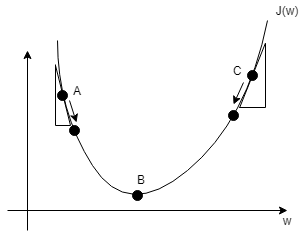
\includegraphics{chapter02/figure/grad_1.png}}
\caption{Đồ thị minh hoạ \textit{gradient decent}.}
\label{fig:grad_1}
\end{figure}

Hình trên là một đồ thị biểu diễn hàm số $J(w)$ có B là điểm tối ưu. Để đến được vị trí B, đầu tiên ta sẽ chọn một điểm bất kì thuộc đồ thị. Sau đó, ta thay đổi vị trí của điểm đó dựa trên giá trị đạo hàm. Việc cập nhật sẽ được lặp lại cho đến khi điểm ta chọn chạy đến vị trí B. Khi đó, ta đã tìm được giá trị tối ưu của hàm $J(w)$

Công thức của \textit{gradient decent} là:
\begin{center}
$w = w - \alpha\frac{\delta J(w)}{\delta w}$
\end{center}

Với $\alpha$ được gọi là \textit{learning rate}, dùng để xác định độ dài bước đi mỗi lần cập nhật và giá trị $\alpha$ luôn lớn hơn $0$.

Nếu ta lấy điểm khởi đầu là A, thì khi đó, đạo hàm tại điểm A sẽ là âm (do $\Delta J(w_{A})$ âm còn $\Delta w_{A}$ dương). Giá trị $w$ được cập nhật sẽ tăng lên (do $-\alpha\frac{\delta J(w_{A})}{\delta w_{A}} > 0$). Ta có thể thấy điểm A sẽ dời về phía bên phải và di chuyển gần hơn đến giá trị tối ưu B.

Trường hợp khác, nếu ta lấy điểm bắt đầu là điểm C, đạo hàm tại điểm C sẽ có giá trị là dương (do $\Delta J(w_{C})$ dương và $\Delta w_{C}$ dương). Giá trị $w$ sẽ giảm xuống (do $-\alpha\frac{\delta J(w_{A})}{\delta w_{A}} < 0$). Điều đó làm cho điểm C sẽ di chuyển về phía bên trái và đến gần hơn với giá trị tối ưu B.

Với số lần lặp vừa đủ và chọn giá trị \textit{learning rate} vừa phải, từ 1 điểm bất kì được chọn trên hàm số, ta đều có thể di chuyển về điểm tối ưu của hàm số.

\begin{figure}[!h]
\centerline{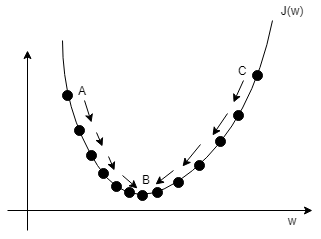
\includegraphics{chapter02/figure/grad_2.png}}
\caption{Kết quả khi sử dụng \textit{gradient decent} để tìm giá trị tối ưu}
\label{fig:grad_2}
\end{figure}

Ta có thể thấy, khi sử dụng \textit{gradient decent}, ta sẽ về được giá trị tối ưu của hàm số dù điểm khởi đầu của ta có thể nằm ở vị trí vào. Như hình \ref{fig:grad_2}, từ điểm A hay C của đồ thị, với số lần lặp vừa đủ và \textit{learning rate} vừa phải, ta sẽ chạy được về điểm tối ưu B của hàm số.

Để sử dụng \textit{gradient decent} tìm giá trị tối ưu, ta phải lựa chọn \textit{learning rate} $\alpha$ không quá lớn hay quá nhỏ. Nếu lựa chọn giá trị $\alpha$ quá lớn, quá trình lặp khi sử dụng \textit{gradient decent} sẽ không chạy về giá trị tối ưu nữa mà sẽ hạy ra xa điểm tối ưu. Còn nếu giá trị $\alpha$ quá nhỏ, số lần lặp để tới được điểm tối ưu sẽ lớn hơn nhiều. Điều này làm cho thời gian chạy để tìm được điểm tối ưu sẽ lâu hơn rất rất nhiều.

\clearpage
\begin{figure}[!htb]
   \begin{minipage}{0.48\textwidth}
     \centering
     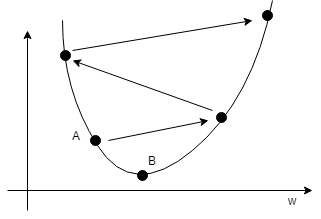
\includegraphics[width=1\linewidth]{chapter02/figure/grad_3.png}
   \end{minipage}\hfill
   \begin{minipage}{0.48\textwidth}
     \centering
     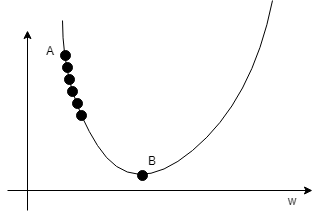
\includegraphics[width=1\linewidth]{chapter02/figure/grad_4.png}
   \end{minipage}
   \caption{\textit{gradient decent} khi giá trị $\alpha$ quá lớn (trái) và quá nhỏ (phải).}
\end{figure}

Với hình bên trái, đây là khi ta lựa chọn giá trị $\alpha$ quá lớn. Với điểm khởi đầu là A, tại đây khi tính đạo hàm và cập nhật hướng về phía bên phải là chính xác, nhưng khi ta thiết lập giá trị $\alpha$ quá lớn, giá trị mới cập nhật sẽ không phải gần hơn đến điểm tối ưu mà còn bước vượt qua điểm tối ưu này. Nếu quá trình trên được lặp lại với $\alpha$ quá lớn, thì càng ngày ra sẽ đi ra xa điểm tối ưu và sẽ không tìm được kết quả mong đợi.

Với hình bên phải, đây là khi ta chọn giá trị $\alpha$ quá nhỏ. Với điểm khởi đầu ngẫu nhiên ta chọn là A, ta vẫn di chuyển về vị trí tối ưu nhưng bởi vì giá trị $\alpha$ quá nhỏ, mỗi lần lặp ta chỉ có thể đi về phía tối ưu một khoảng quá ngắn. Vì vậy để về điểm tối ưu, ta phải lặp đi lặp lại quá nhiều bước. Kết quả là thời gian ta đến được điểm cần tìm quá lâu cũng như quá tốn tài nguyên tính toán.

Vì thế, để giải thuật \textit{gradient decent} chạy tốt, ta cần phải lựa chọn giá trị $\alpha$ cho phù hợp để có thể tìm được giá trị tối ưu một cách nhanh nhất và chính xác.

\textit{Gradient decent} cũng chỉ có thể tìm được điểm tối ưu khi hàm số thoả mãn những yêu cầu nhất định. Đó chính là khả vi và phải là hàm lồi. Nếu không thoả mãn 2 yếu tố trên, giải thuật này sẽ không tìm được điểm tối ưu.

Với yếu tố khả vi, ta có thể thấy việc chỉ ra hướng để đi đến điểm tối ưu của \textit{gradient decent} dựa trên giá trị của đạo hàm ($w = w - \alpha\frac{\delta J(w)}{\delta w}$). Nếu hàm số không khả vi, là ta sẽ không thể tính được giá trị $\frac{\delta J(w)}{\delta w}$ cũng như việc tìm được điểm tối ưu là không khả thi.

Với yếu tố hàm số phải là hàm lồi, đây là yếu tố quan trọng để xác định xem ta có thể tìm được điểm tối ưu của hàm số hay không. Vì nếu không là hàm lồi, tuỳ thuộc vào vị trí khởi tạo mà giá trị tối ưu ta thu được sau khi sử dụng \textit{gradient decent} có thể là điểm tối ưu cục bộ, không phải điểm tối ưu toàn cục.

\begin{figure}[!h]
\centerline{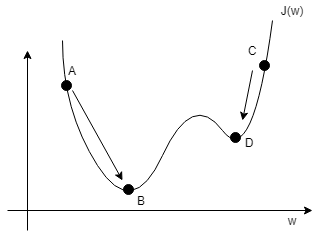
\includegraphics{chapter02/figure/grad_5.png}}
\caption{Sử dụng \textit{
gradient decent} không hàm số không là hàm lồi}
\label{fig:grad_5}
\end{figure}

Đồ thị trên là đồ thị của một hàm không là hàm lồi. Những hàm này ngoài điểm tối ưu toàn cục thì còn có các điểm tối ưu cục bộ. Nếu ta lấy điểm khởi đầu là điểm A, thì sau khi sử dụng \textit{gradient decent}, điểm tối ưu ta tìm được vẫn là điểm tối ưu toàn cục là điểm B. Nhưng nếu điểm khởi đầu của chúng ta là điểm C. Khi đó, sau khi dùng \textit{gradient decent} thì điểm tối ưu mà ta tìm được chính là điểm D, và D không là điểm tối ưu cục bộ của hàm. Vì thế, khi sử dụng \textit{gradient decent} với hàm số không là hàm lồi, giá trị tối ưu ta tìm được có thể không là điểm tối ưu toàn cục.

Trên thực tế, khi sử dụng \textit{gradient decent}, ta chỉ có thể tìm được vị trí gần với điểm tối ưu cục bộ.

\clearpage
\begin{figure}[!h]
\centerline{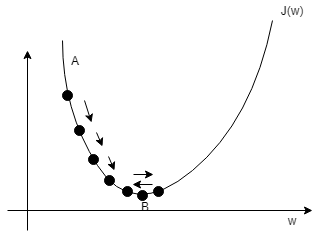
\includegraphics{chapter02/figure/grad_6.png}}
\caption{Kết quả của \textit{gradient decent} thực tế}
\label{fig:grad_6}
\end{figure}

Như hình trên, ta lấy điểm khởi đầu là A. Sau đó, sử dụng \textit{gradient decent} để tìm giá trị tối ưu. Khi này, kết quả của chúng ta sẽ chạy lại gần điểm B. Nhưng, khi lại gần B đến một khoảng nhất định, thì khi ta cập nhật giá trị sau khi sử dụng \textit{gradient decent}, kết quả là ta sẽ vượt qua giá trị tối ưu 1 khoảng rất nhỏ. Và khi ta lặp lại \textit{gradient decent} 1 lần nữa, thì ta sẽ đi qua điểm tối ưu 1 khoảng nhỏ tiếp tục. Và cứ như thế, khi chạy \textit{gradient decent}, kết quả mà ta nhận được sẽ dao động môt khoảng nhỏ xung quanh giá trị tối ưu B. Nhưng giá trị sai khác khi ta dùng \textit{gradient decent} và giá trị tối ưu là rất nhỏ. Vì thế, kết quả ta thu được sau khi sử dụng \textit{gradient decent} vẫn rất tốt khi áp dụng vào các bài toán tìm giá trị tối ưu.

Quay trở lại với bài toán tìm giá trị nhỏ nhất của hàm \textit{cost function}, hàm số của chúng ta gồm 2 biến đó chính là $w$ và $b$. Vì thế, mỗi lần lặp của \textit{gradient decent}, ta cần phải cập nhật giá trị của cả $w$ và $b$ bằng cách sử dụng đạo hàm từng phần hàm số với lần lượt 2 biến.

Với \textit{cost function}:
\begin{center}
$J(w, b) = \frac{-1}{m}\sum_{i=1}^{m}y^{(i)}\log \hat{y}^{(i)}+(1-y^{(i)})\log (1-\hat{y}^{(i)})$
\end{center}

Ta sẽ sử dụng đạo hàm từng phần với mỗi biến của \textit{cost function} là $w$ và $b$. Kết quả cập nhật của mỗi biến qua mỗi lần lặp của \textit{gradient decent} là:
\begin{center}
$w = w - \alpha\frac{\delta J(w, b)}{\delta w}$\\
$b = b - \alpha\frac{\delta J(w, b)}{\delta b}$
\end{center}

Ta cập nhật giá trị của $w$ và $b$ với số lần lặp vừa đủ cùng $\alpha$ vừa phải sẽ tìm ra được giá trị tối ưu của hàm \textit{cost function}. Để tính được giá trị của $\frac{\delta J(w, b)}{\delta w}$ và $\frac{\delta J(w, b)}{\delta b}$, ta có thể dùng \textit{computation graph} để tìm được các giá trị đó.

\section{Cách tính đạo hàm riêng dưới góc nhìn Computation graph}
\textit{Computation graph} là một phương pháp giúp tìm đạo hàm riêng một biến của hàm số. Hàm được biểu diễn thành một đồ thị với các đỉnh con là kết quả phép tính của 2 đỉnh cha. Ta sẽ tính giá trị đạo hàm tại mỗi đỉnh của đồ thị bằng cách lấy giá trị xấp xỉ và lan truyền ngược giá trị về đỉnh cha cho đến biến mà ta cần tính đạo hàm. Ta sẽ xem qua ví dụ về việc sử dụng \textit{computation graph} để tính đạo hàm riêng.
\begin{figure}[!h]
\centerline{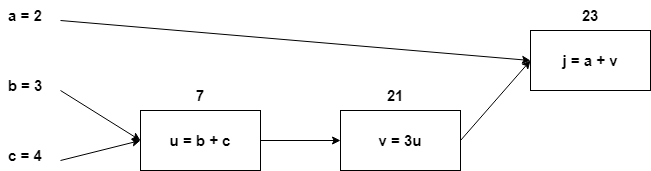
\includegraphics[scale=0.5]{chapter02/figure/com_1.png}}
\caption{Ví dụ sử dụng \textit{computation graph} để tính đạo hàm}
\label{fig:com_1}
\end{figure}

Hình trên biểu diễn một hàm số $J$ sử dụng \textit{computation graph}. Hàm số được chia nhỏ thành từng phần và giá trị mỗi phần được tính với các giá trị a, b, c được cho trước. Hàm $J$ có phương trình là:
\begin{equation}
\label{sec2:eqn6}
J = a + 3(b + c) 
\end{equation}

Ta chia nhỏ biểu thức \ref{sec2:eqn6} trên bằng các biểu thức nhỏ hơn:
\begin{align}
\label{sec2:eqn7}
u &= b + c\\
\label{sec2:eqn8}
v &= 3u\\
\label{sec2:eqn9}
J &= a + v 
\end{align}

Với mỗi biểu thức trên là một đỉnh của đồ thị, ta sẽ được một \textit{computation graph} như hình trên. Tiếp theo, ta sẽ tính đạo hàm tại mỗi đỉnh bằng cách xấp xỉ và lan truyền giá trị ngược lại.

%Với hàm số $f(h(x))$, ta có thể tính đạo hàm của $x$ theo $f$ bằng cách:
%\begin{center}
%$\frac{\delta f}{\delta x} = \frac{\delta f}{\delta h}\frac{\delta h}{\delta x}$
%\end{center}
%Lấy ví dụ ta tính đạo hàm của $a$ theo $J$ tại $a=2$. Dựa vào công thức trên, ta có đạo hàm của $J$ theo $a$ là:
%\begin{center}
%$\frac{\delta J}{\delta a} = \frac{\delta J}{\delta v}\frac{\delta v}{\delta a}$
%\end{center}
Ta sẽ tính đạo hàm tại $a=2$ bằng phương pháp xấp xỉ. Ta chọn $a_{1}$ sao cho $\Delta a$ rất nhỏ ($0.001$). Ta lấy $a_{1} = 2.001$.Từ biểu thức \ref{sec2:eqn9}, suy ra:
\begin{equation}
\label{sec2:eqn10}
J_{1} = a_{1} + v = 23.001
\end{equation}

Ta tính giá trị đạo hàm của $J$ theo $a$ và $J_{1}$ từ \ref{sec2:eqn10}:
\begin{equation}
\label{sec2:eqn11}
\frac{\Delta J}{\Delta a} = \frac{J_{1} - J}{a_{1} - a} = \frac{23.001-23}{2.001-2} = 1\\
\end{equation}

%Sau đó, ta lan truyền kết quả lên để tính đạo hàm của $J$ theo $a$ dựa trên đạo hàm của $J$ theo $v$ và đạo hàm của $v$ theo $a$:
%\begin{center}
%$\frac{\Delta v}{\Delta a} = \frac{v_{1} - v}{a_{1} - a} = \frac{11.001-11}{5.001-5} = 1$\\
%\end{center}
Ta có thể xấp xỉ $\frac{\Delta J}{\Delta a}$ bằng $\frac{\delta J}{\delta a}$. Từ \ref{sec2:eqn11}, giá trị đạo hàm của $J$ tại $a=2$ xấp xỉ:
\begin{center}
$\frac{\Delta J}{\Delta a} = 1$.\\
\end{center}

Ta sẽ sử dụng cách tương tự để tính giá trị đạo hàm của $J$ tại $b=3$ cũng như $c=4$. Với $b=3$, ta chọn $b_{1} = 3.001$. Từ \ref{sec2:eqn7}, \ref{sec2:eqn8}, \ref{sec2:eqn9} suy ra:
\begin{align}
u_{1} = b_{1} + c &= 7.001\\
v_{1} = 3u_{1} &= 21.003\\
J_{1} = av_{1} &= 23.003
\end{align}

Ta tính giá trị đạo hàm của $J$ theo $v$:
\begin{equation}
\label{sec2:eqn15}
\frac{\Delta J}{\Delta v} = \frac{J_{1} - J}{v_{1} - v} = \frac{23.003-33}{21.003-21} = 1
\end{equation}

Sau đó, ta lan truyền kết quả lên để tính đạo hàm của $J$ theo $u$ dựa trên đạo hàm của $J$ theo $v$ từ \ref{sec2:eqn15} và đạo hàm của $v$ theo $u$:
\begin{align}
\frac{\Delta v}{\Delta u} &= \frac{v_{1} - v}{u_{1} - u} = \frac{21.003-21}{7.001-7} = 3\\
\label{sec2:eqn17}
\frac{\Delta J}{\Delta u} &= \frac{\Delta J}{\Delta v}\frac{\Delta v}{\Delta u} = 1x3 = 3
\end{align}

Sau đó, ta lan truyền kết quả lên để tính đạo hàm của $J$ theo $b$ dựa trên đạo hàm của $J$ theo $u$ từ \ref{sec2:eqn17} và đạo hàm của $u$ theo $b$:
\begin{align}
\frac{\Delta u}{\Delta b} &= \frac{u_{1} - u}{b_{1} - b} = \frac{7.001-7}{3.001-3} = 1\\
\label{sec2:eqn19}
\frac{\Delta J}{\Delta b} &= \frac{\Delta J}{\Delta u}\frac{\Delta u}{\Delta b} = 3x1=3.
\end{align}

Từ \ref{sec2:eqn19}, giá trị đạo hàm của $J$ tại $b=3$ xấp xỉ bằng 3.

Cuối cùng, với $c=4$, ta chọn $c_{1} = 4.001$. Từ \ref{sec2:eqn7}, \ref{sec2:eqn8}, \ref{sec2:eqn9} suy ra:
\begin{align}
u_{1} &= b + c_{1} = 7.001\\
v_{1} &= a + u_{1} = 21.003\\
J_{1} &= 3v_{1} = 23.003
\end{align}

Ta tính giá trị đạo hàm của $J$ theo $v$:
\begin{equation}
\label{sec2:eqn23}
\frac{\Delta J}{\Delta v} = \frac{J_{1} - J}{v_{1} - v} = \frac{23.003-33}{21.003-21} = 1\\
\end{equation}

Sau đó, ta lan truyền kết quả lên để tính đạo hàm của $J$ theo $u$ dựa trên đạo hàm của $J$ theo $v$ từ \ref{sec2:eqn23} và đạo hàm của $v$ theo $u$:
\begin{align}
\frac{\Delta v}{\Delta u} = \frac{v_{1} - v}{u_{1} - u} = \frac{21.003-21}{7.001-7} = 3\\
\label{sec2:eqn25}
\frac{\Delta J}{\Delta u} = \frac{\Delta J}{\Delta v}\frac{\Delta v}{\Delta u} = 1x3 = 3
\end{align}

Sau đó, ta lan truyền kết quả lên để tính đạo hàm của $J$ theo $c$ dựa trên đạo hàm của $J$ theo $u$ từ \ref{sec2:eqn25} và đạo hàm của $u$ theo $c$:
\begin{align}
\frac{\Delta u}{\Delta c} = \frac{u_{1} - u}{c_{1} - c} = \frac{7.001-7}{4.001-4} = 1\\
\label{sec2:eqn27}
\frac{\Delta J}{\Delta c} = \frac{\Delta J}{\Delta u}\frac{\Delta u}{\Delta c} = 3x1=3
\end{align}

Từ \ref{sec2:eqn27}, giá trị đạo hàm của $J$ tại $c=4$ xấp xỉ bằng 3.

Ta sẽ sử dụng phương pháp này để tính đạo hàm cho \textit{gradient decent}.\\ \textit{Loss function} của \textit{logistic regression} với 2 \textit{feature}:
\begin{equation}
\label{sec2:eqn28}
\mathcal{L}(a, y) = -(y\log (a) + (1-y)\log (1-a))
\end{equation}
Với:
\begin{align}
a = \hat{y} = \sigma (z) = \frac{1}{1+e^{-z}}\\
z = w^{T}x + b
\end{align}

Ta có đồ thị của \textit{computation graph} như sau:
\begin{figure}[!h]
\centerline{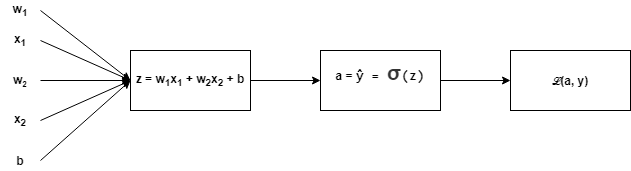
\includegraphics[scale=0.5]{chapter02/figure/com_2.png}}
\caption{Sử dụng \textit{computation graph} vào \textit{logistic regression}}
\label{fig:com_2}
\end{figure}

Ta tính đạo hàm của $\mathcal{L}$ theo $a$ từ \ref{sec2:eqn28}:
\begin{equation}
\label{sec2:eqn31}
\frac{\partial \mathcal{L}}{\partial a} = -(y\frac{1}{a} + (1-y)\frac{-1}{1-a}) = \frac{1-y}{1-a} - \frac{y}{a} = \frac{a(1-y) - y(1-a)}{a(1-a)} = \frac{a-y}{a(1-a)}
\end{equation}

Sau đó, ta lan truyền kết quả lên để tính đạo hàm của $\mathcal{L}$ theo $z$ dựa trên đạo hàm của $\mathcal{L}$ theo $a$ từ \ref{sec2:eqn31} và đạo hàm của $a$ theo $z$:
\begin{align}
\frac{\partial a}{\partial z} &=  \frac{0(1 + e^{-z}) - (-e^{-z})1}{(1+e^{-z})^{2}} = \frac{e^{-z}}{(1+e^{-z})^{2}} = \frac{1}{1+e^{-z}\frac{e^{-z}}{1+e^{-z}}} = \frac{1}{1+e^{-z}}\frac{1+e^{-z}-1}{1+e^{-z}} = a(1-a)\\
\label{sec2:eqn33}
\frac{\partial \mathcal{L}}{\partial z} &= \frac{\partial \mathcal{L}}{\partial a}\frac{\partial a}{\partial z} = \frac{a-y}{a(1-a)}a(1-a) = a-y
\end{align}

Sau đó, ta lan truyền kết quả lên để tính đạo hàm của $\mathcal{L}$ theo $w_{1}$, $w_{2}$, $b$ dựa trên đạo hàm của $\mathcal{L}$ theo $z$ từ \ref{sec2:eqn33} và đạo hàm của $z$ theo $w_{1}$, $w_{2}$, $b$:
\begin{align}
\label{sec2:eqn34}
\frac{\partial z}{\partial w_{1}} &=  x_{1} \nonumber\\
\frac{\partial \mathcal{L}}{\partial w_{1}} &= \frac{\partial \mathcal{L}}{\partial z}\frac{\partial z}{\partial w_{1}} = (a-y)x_{1}\\
\label{sec2:eqn35}
\frac{\partial z}{\partial w_{2}} &=  x_{2} \nonumber\\
\frac{\partial \mathcal{L}}{\partial w_{2}} &= \frac{\partial \mathcal{L}}{\partial z}\frac{\partial z}{\partial w_{2}} = (a-y)x_{2}\\
\label{sec2:eqn36}
\frac{\partial z}{\partial b} &=  1 \nonumber\\
\frac{\partial \mathcal{L}}{\partial b} &= \frac{\partial \mathcal{L}}{\partial z}\frac{\partial z}{\partial b} = (a-y)
\end{align}

Suy ra, công thức \textit{computation graph} cho \textit{loss function} từ \ref{sec2:eqn34}, \ref{sec2:eqn35}, \ref{sec2:eqn36} là:
\begin{align}
\label{sec2:eqn37}
w_{1} = w_{1} - \alpha\frac{\partial \mathcal{L}}{\partial w_{1}} = w_{1} - \alpha(a-y)x_{1}\\
\label{sec2:eqn38}
w_{2} = w_{2} - \alpha\frac{\partial \mathcal{L}}{\partial w_{2}} = w_{2} - \alpha(a-y)x_{2}\\
\label{sec2:eqn39}
b = b - \alpha\frac{\partial \mathcal{L}}{\partial b} = b - \alpha(a-y)
\end{align}

\textit{Cost function} là tổng các \textit{loss funtion} của mỗi dữ liệu:
\begin{equation}
\label{sec2:eqn40}
J(w,b) = \frac{1}{m}\sum_{i=1}^{m}\mathcal{L}(a^{i}, x^{i}) 
\end{equation}

Từ đó, ta có thể tính được \textit{gradient decent} của \textit{cost function} bằng cách tính tổng \textit{gradient decent} các \textit{loss function} của dữ liệu từ \ref{sec2:eqn37}, \ref{sec2:eqn38}, \ref{sec2:eqn39}, \ref{sec2:eqn40}:
\begin{center}
$w_{1} = w_{1} - \alpha\frac{\partial J(w,b)}{\partial w_{1}} = w_{1} - \alpha\sum_{i=1}^m\frac{\partial \mathcal{L} (a^{i}, y^{i})}{\partial w_{1}} = w_{1} - \alpha\sum_{i=1}^m(a^{i} - y^{i})x_{1}^{i}$\\
$w_{2} = w_{2} - \alpha\frac{\partial J(w,b)}{\partial w_{2}} = w_{2} - \alpha\sum_{i=1}^m\frac{\partial \mathcal{L}(a^{i}, y^{i})}{\partial w_{2}} = w_{2} - \alpha\sum_{i=1}^m(a^{i} - y^{i})x_{2}^{i}$\\
$b = b - \alpha\frac{\partial J(w,b)}{\partial b} = b - \alpha\sum_{i=1}^m\frac{\partial \mathcal{L(a^{i}, y^{i})}}{\partial b} = b - \alpha\sum_{i=1}^m(a^{i} - y^{i})$
\end{center}

Một cách tổng quát hơn, với một dữ liệu gồm $n$ \textit{feature}, ta có \textit{gradient decent} là:
\begin{center}
$w_{1} =  w_{1} - \alpha\sum_{i=1}^m(a^{i} - y^{i})x_{1}^{i}$\\
$w_{2} =  w_{2} - \alpha\sum_{i=1}^m(a^{i} - y^{i})x_{2}^{i}$\\
\quad     \vdots\\
$w_{n} = w_{n} - \alpha\sum_{i=1}^m(a^{i} - y^{i})x_{n}^{i}$\\
$b =  b - \alpha\sum_{i=1}^m(a^{i} - y^{i})$
\end{center}

\section{Tổng kết phương pháp Logistic Regression}
Dưới đây là thuật giải của \textit{logistic regression} bằng mã giả:
\clearpage
\begin{algorithm}[!h]
\caption{Logistic regression}
$num\_iter=500, w1 = 0, w2 = 0, ..., wn = 0, b = 0, alpha = 0.1$\\
\For{ $i\gets1$ \KwTo $range(num_iter)$}{
    $J = 0, dw1 = 0, dw2 = 0, ..., dwn = 0, db = 0$\\
    \For{ $j\gets1$ \KwTo $m$}{
        $z = w1*xj1 + w2*xj2 + ... + wn*xjn + b$\\
        $a = 1/(1 + e^(-z))$\\
        $J += -(yj*log(aj) + (1 - yj)*log(1 - aj)$\\
        $dz = aj - yj$\\
        $dw1 += dz*xj1$\\
        $dw2 += dz*xj2$\\
        ...\\
        $dwn += dz*xjn$\\
        $db += dz$\\
    }
    $J/=m$\\
    $dw1/=m$\\
    $dw2/=m$\\
    ...\\
    $dwn/=m$\\
    $db/=m$\\
    $w1 = w1 - alpha*dw1$\\
    $w2 = w2 - alpha*dw2$\\
    ...\\
    $wn = wn - alpha*dwn$\\
    $b = b - alpha*b$
}
\end{algorithm}

Đoạn code trên là mã giả dùng để trình bày ý tưởng hiện thực \textit{logistic regression}. Ta xét trên một tập dữ liệu gồm $m$ dữ liệu và mỗi dữ liệu gồm $n$ \textit{feature}. Đầu tiên, chúng ta sẽ khai báo cáo biến cần thiết. Các $w1$, $w2$, ..., $wn$ lần lượt là các trọng số của mỗi \textit{feature} thuộc dữ liệu. $b$ là \textit{bias} được thêm vào. Giá trị num\_iter là số lần lặp để tìm được giá trị tối ưu của \textit{cost function}. Đây là giá trị ta có thể tuỳ chỉnh. Ta có thể gán 40, 50 hay 500 thâm chí đến 10000 tuỳ thuộc vào số lần lặp cần thiết để tìm được giá trị tối ưu của \textit{cost function}. $alpha$ là \textit{learning rate} mà ta thiết lập cho \textit{gradient decent}. Giá trị này không nên quá nhỏ hoặc quá lớn.

Tiếp theo, ta tính \textit{gradient decent} của \textit{cost function} bằng cách lặp lại việc cập nhật các trọng số với số lần lặp num\_iter cho trước.

Trong mỗi lần lặp, ta sẽ khởi tạo giá trị của \textit{cost function} $J$, các giá trị đạo hàm của $J$ theo $w1, w2, ..., wn$ là $dw1, dw2, ..., dwn$ và đạo hàm của $J$ theo $b$ là $wb$.

Ta sẽ chạy qua từng dữ liệu trong tập dữ liệu cho trước. Ta tính giá trị đầu ra. Tiếp đến, ta tính sự sai biệt giữa giá trị tính toán và giá trị thực tế dựa trên \textit{cross-entropy} và thêm kết quả vào \textit{cost function}. Sau khi chạy qua hết tập dữ liệu, ta tính giá trị đạo hàm của $J$ theo từng trọng số theo công thức được suy ra từ phần trước. Cuối cùng, ta cập nhật giá trị các trọng số dựa trên đạo hàm của chúng theo \textit{gradient decent}. Quá trình trên sẽ được lặp lại cho đến khi ta tìm được giá trị tối ưu của \textit{cost function} và thu được bộ trọng số thoả mãn yêu cầu.

\newpage
\section{Bài tập}
\begin{exer}
Từ dữ liệu của ví dụ \ref{exmp:o}, ta lấy một tập dữ liệu huấn luyện có kích thước m = 4, như bảng \ref{tab:exercise}: 
\begin{table*}[ht]
\centering
\begin{tabular}{|l|l|l|l|}
\hline
Height & Gender \\ \hline
1.5   & F \\ \hline
1.75  & M \\ \hline
1.6     & M \\ \hline
1.45  & F  \\ \hline
\end{tabular}
\caption{Dữ liệu đầu vào của bài tập}
\label{tab:exercise}
\end{table*}

Sử dụng mô hình Logistic Regression $h\theta(x) = g(\theta_0 + \theta_1x_1)$ để giải bài toán phân loại Nam (M) và Nữ (F) dựa theo chiều cao của họ, với $x_1$ là vector chiều cao những người trong tập dữ liệu, $g$ là hàm sigmoid, và $\theta_0$, $\theta_1$ là hai trọng số cần phải học. Giả sử $y = 0$ khi một là nữ và $y = 1$ khi một người là nam, \textit{learning rate} $\alpha = 0.1$ và giá trị khởi tạo của $\theta_0$, $\theta_1$ là  $0$,  hàm mất mát là hàm \textit{Cross-Entropy}. Với tập dữ liệu training như bảng \ref{tab:exercise} và sử dụng mô hình Logistic Regression để cập nhật trọng số $\theta_0$ và $\theta_1$, hãy cho biết giá trị của hai trọng số $\theta_0$ và $\theta_1$ sau 2 lần lặp?
\end{exer}

\begin{exer}
Cho phương trình $J = a + 5(b + cd)$

Hãy vẽ computation graph của phương trình trên và tính đạo hàm của $J$ tại từng biến $a, b, c, d$ với $a=5, b=6, c=7, d=8$.
\end{exer}
\chapter{Multi Layer Perceptron và Deep Learning}
\label{chp:03}

\section{Logistic regression dưới góc nhìn neural network}
\label{sec31}
\textit{Hồi quy logistic} (logistic regression) là một \textit{phương pháp phân loại nhị phân} (binary classification method), được xây dựng bởi một hàm có khả năng nhận một giá trị bất kỳ và trả kết quả ra một con số nằm giữa 0 và 1 (hàm sigmoid). Điều này cũng tương tự như một \textit{mạng nơ-ron} (neural network) một lớp. Hình \ref{fig:LogisticRegressionNN} minh họa cho việc dùng hồi quy logistic như một mạng nơ-ron đơn giản.

\begin{figure}[!h]
	\centering
		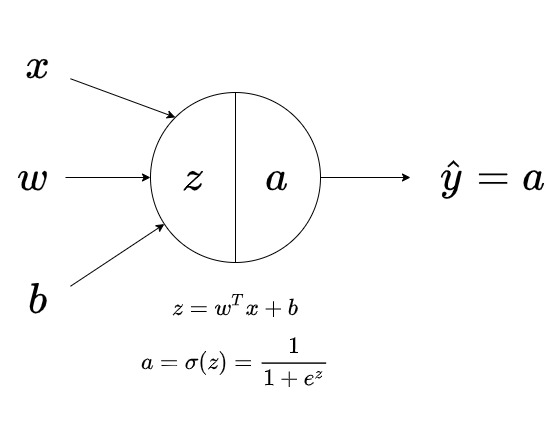
\includegraphics[width=0.5\columnwidth]{chapter03/figure/LogisticRegressionNN.jpg}
        \caption{Một mạng nơ-ron đơn giản.}
        \label{fig:LogisticRegressionNN}
		\centering
\end{figure}

Trong hình \ref{fig:LogisticRegressionNN}, ma trận $x$ chứa các \textit{thuộc tính} (feature) của một input, ma trận $w$ sẽ là trọng số các thuộc tính và $b$ là bias. Sau khi trải qua các bước tính toán, kết quả thu được $\hat{y}$ sẽ là xác suất \textit{nhãn} (label) $y$ nhận giá trị bằng 1 với $x$ và $w$ đã biết.
\[ P(y=1|w,x) = \hat{y}\]

Như đã trình bài ở trên, kết quả của hàm $\sigma$ luôn là một giá trị từ 0 đến 1. Nhưng giá trị của nhãn thì luôn là 0 hoặc 1. Sự sai biệt này dẫn đến khái niệm \textit{hàm mất mát} (loss function). Có rất nhiều hàm có thể được dùng để làm hàm mất mát, tuy nhiên trong chương này ta sẽ chỉ dùng \textit{ hàm mất mát Cross-entropy} (Cross-entropy loss function) được định nghĩa như sau.
\[ L(\hat{y},y) = -  [y\log{\hat{y}} + (1-y)\log{(1-\hat{y})}] \]

Giá trị của hàm mất mát là kết quả của \textit{lan truyền xuôi} (forward propagation) và đóng vai trò then chốt trong quá trình \textit{lan truyền ngược} (backward propagation).

\begin{figure}[!h]
	\centering
		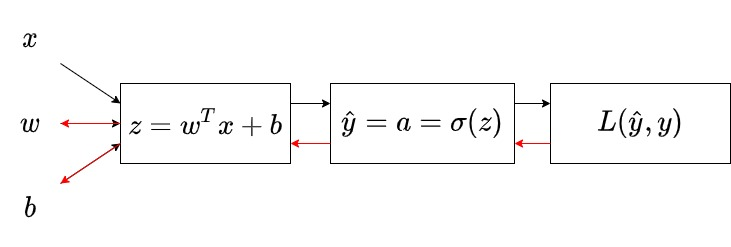
\includegraphics[width=0.5\columnwidth]{chapter03/figure/Back-fowardPropagation.jpg}
        \caption{Lan truyền xuôi và lan truyền ngược.}
        \label{fig:backfowardPropagation}
		\centering
\end{figure}

Quan sát hình \ref{fig:backfowardPropagation}, quá trình lan truyền ngược và cập nhật trọng số bằng \textit{gradient descent} được thực hiện như sau (giả sử $w$ có kích thước $1\times n$):

1.$\indent $ Tính đạo hàm riêng phần của $L(\hat{y},y)$ theo $w_i$ (với $i=1...n$).
    \begin{align*}
        \frac{\partial L}{\partial w_i} &= \frac{\partial L}{\partial a}\times\frac{\partial a}{\partial w_i } \\
        &= \frac{\partial L}{\partial a}\times \frac{\partial a}{\partial z} \times \frac{\partial z}{\partial w_i}\\
        &= (\frac{1-y}{1-a}-\frac{y}{a})\times \frac{\partial a}{\partial z} \times \frac{\partial z}{\partial w_i}\\
        & = (\frac{1-y}{1-a}-\frac{y}{a}) \times a \times (1-a)\times \frac{\partial z}{\partial w_i}\\
        & =  (\frac{1-y}{1-a}-\frac{y}{a}) \times a \times (1-a)\times x_i\\
        &= (a-y) \times x_i\\
        &= (\hat{y}-y) \times x_i
    \end{align*}

2.$\indent$ Cập nhật lại trọng số bằng gradient descent:
\begin{align*}
    w_i &= w_i - \alpha \times \frac{\partial L}{\partial w_i}\\
    &= w_i - \alpha \times(\hat{y}-y) \times x_i
\end{align*}

Cách cập nhật trọng số được trình bày ở trên xét trên mà trên $x$ có kích thước $1\times n$. Trường hợp $x$ có kích thước $m \times n$, ta sẽ áp dụng gradient descent với $\frac{\partial J}{\partial w_i}$ thay vì $\frac{\partial L}{\partial w_i}$. Trong đó, J là \textit{cost} được tính theo công thức sau (với $y^{(i)}$ và  $\hat{y}^{(i)}$ lần lượt là nhãn và kết quả dự đoán của $x^{i}$):
\[J = -\frac{1}{m} \times \sum_{i=1}^{m}L(\hat{y}^{(i)},y^{(i)})\]
%%%%%%%%%%%%%%%%%%%%%%%%%%%%%%%%%%%%%%%%%%%%%%%%%%%%%%%%%%

\section{Mạng neural network nhiều lớp(MLP) và mạng học sâu}
\subsection{Nhắc lại mạng neural network nhiều lớp}
Như chương trước đã đề cập, mạng neural network nhiều lớp thực chất chỉ gồm nhiều tầng mà trong mỗi tầng các perceptron đặt chồng lên nhau. Cách thức hoạt động của những tầng mạng cũng rất đơn giản bằng cách nhân ma trận. Bằng cách này, chúng ta có thể giải quyết rất nhiều bài toán. Tuy nhiên, khi để ý thì tất cả các phép tính này đều xây dựng trên hàm tuyến tính. Điều này gây ra những vấn đề sau:
\begin{itemize}
    \item Khó khăn trong việc xây dựng những mô hình phi tuyến phức tạp.
    \item Khi đi qua nhiều lớp, những vấn đề về trọng số sẽ xảy ra ví dụ như đầu ra của một perceptron nào đó quá lớn hoặc quá âm sẽ ảnh hưởng rất nhiều đến độ chính xác của bài toán hoặc thậm chí là máy tính không thể biểu diễn được.
    \item Vì đầu ra sẽ được so sánh về ngưỡng nào đó, do đó, vấn đề về xác định xác suất sẽ rất khó thực hiện vì chúng ta chỉ thể hiện được mức độ hay nói cách khác là những giá trị rời rạc. Ví dụ như chúng ta muốn nhận diện chó hoặc mèo, thì mô hình xây dựng trên MLP chỉ cho phép ta biết đó là chó hoặc mèo chứ không cho ta biết xác suất mà mô hình nhận diện được vật thể đó là chó là bao nhiêu phần trăm.
\end{itemize}

\subsection{Sự tiến hóa của mạng neural netwwork nhiều lớp}
Sau những vấn đề được nêu ra ở trên thì chúng ta thấy rằng, vấn đề đang nằm ở hàm activation và nó cần được thay đổi. Nhưng thay đổi làm sao và thế nào lại là một câu hỏi khó.

Không sao cả, vấn đề chỗ nào thì chúng ta sẽ đi gỡ rối chỗ đó tương ứng như sau. 
\begin{itemize}
    \item Do việc xây dựng MLP như trên đang theo mô hình tuyến tính đối với 2 tầng gần nhau. Do đó, dễ nghĩ đến là chúng ta sẽ thiết kế một hàm activation phi tuyến. (1)
    \item Khi đi qua nhiều lớp, những vấn đề về trọng số sẽ xảy ra ví dụ như đầu ra của một perceptron nào đó quá lớn hoặc quá âm sẽ ảnh hưởng rất nhiều đến độ chính xác của bài toán. Để giải quyết điều này, chúng ta sẽ đi tìm hàm sao cho có thể kéo những giá trị đầu ra về 1 khoảng nào đó có thể kiểm soát được và có ý nghĩa trong xác suất thống kê như (-1,1) hoặc (0,1). (2)
    \item Vấn đề thể hiện độ tin cậy mà mô hình cho ra sẽ cho chúng ta ý tưởng về thiết kế hàm activation sao cho kết quả cho ra nằm trong khoảng (0,1) thể hiện cho xác suất. (3) 
\end{itemize}

Từ (1),(2),(3) chúng ta sẽ thiết kế hàm activation sao cho đó là hàm phi tuyến (hàm này sẽ phải có đạo hàm) và đầu ra nên có giá trị (-1,1) hoặc (0,1).

Sau một thời gian phát triển, các mạng học sâu đã ra đời và dựa trên những hàm activation này.

\subsection{Mạng học sâu}
Bằng cách áp dụng các hàm activation khác nhau thay cho threshold và cách làm tuyến tính như MLP thì mạng học sâu đã ra đời. Chúng ta cũng dễ thấy rằng, không có sự khác biệt quá nhiều giữa MLP và mạng học sâu (như hình minh họa) hay có thể nói MLP là một tập hợp con của mạng học sâu khi chúng ta chỉ cần thay đổi activation của từng hidden layers và layer đầu ra để thể hiện về tính phi tuyến và xác suất.

\begin{figure}[!h]
	\centering
		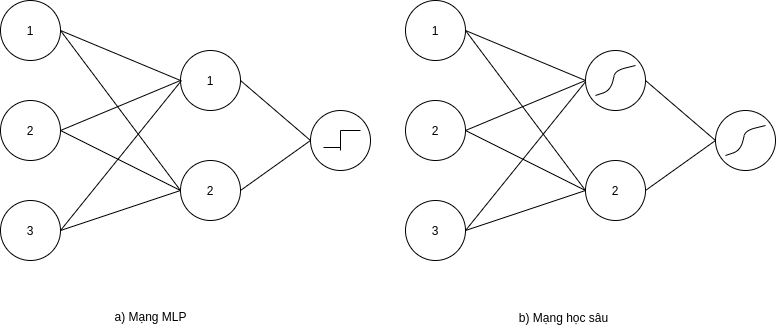
\includegraphics[width=10cm, height=5cm]{chapter03/figure/neuralnetwork.png}
        \caption{Hình a) miêu tả mạng MLP với 1 hidden layer, hình b) miêu tả mạng học sâu với 1 hidden layer}
        \label{fig:neuralnetwork}
		\centering
\end{figure}

Như hình trên, chúng ta có thể thấy rằng, đi qua mỗi layer của mạng học sâu chúng ta có thể thêm vào đó các hàm activation khác nhau, hoặc thậm chí không cần thêm. Còn trong MLP thì chỉ đơn thuần là các phép tính toán ma trận tuyến tính.

\section{Các hàm activation functions}
\subsection{Hàm sigmoid}
$\indent$\textbf{Công thức:}
\[ \sigma(x) = \frac{1}{1+e^{-x}} \]
$\indent$Hàm sigmoid nhận vào một giá trị thực $x$ và trả về một giá trị trong khoảng $(0,1)$. Nếu $x$ là một số thực âm rất nhỏ thì kết quả của hàm sigmoid sẽ tiệm cận 0, và ngược lại nếu $x$ là một số dương rất lớn thì kết quả sẽ tiệm cận 1. Hình \ref{fig:HamSigmoid} bên dưới là đồ thị biểu diễn cho hàm sigmoid.

\begin{figure}[!h]
	\centering
		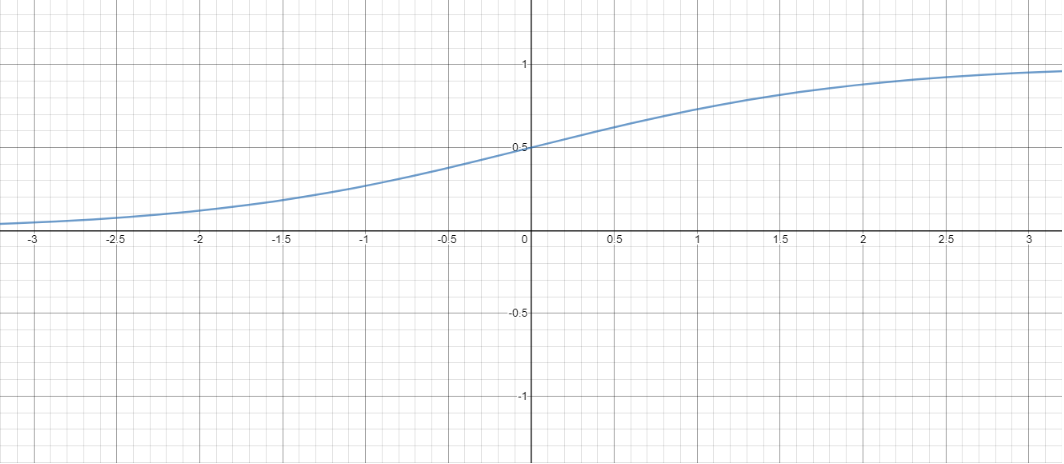
\includegraphics[width=0.75\columnwidth]{chapter03/figure/HamSigmoid.png}
        \caption{Đồ thị của hàm sigmoid.}
        \label{fig:HamSigmoid}
		\centering
\end{figure}

Như đã thấy ở phần \ref{sec31}, khi sử dụng hàm sigmoid làm hàm activation, việc tính toán vô cùng thuận lợi do kết quả đạo hàm của sigmoid rất "đẹp". Tuy nhiên, điều này không thể che lấp những khuyết điểm nghiêm trọng của sigmoid:

\begin{enumerate}
    \item \textbf{Hàm sigmoid bão hòa và \textit{triệt tiêu gradient} (vanishing gradient)}
    \begin{figure}[!h]
	\centering
		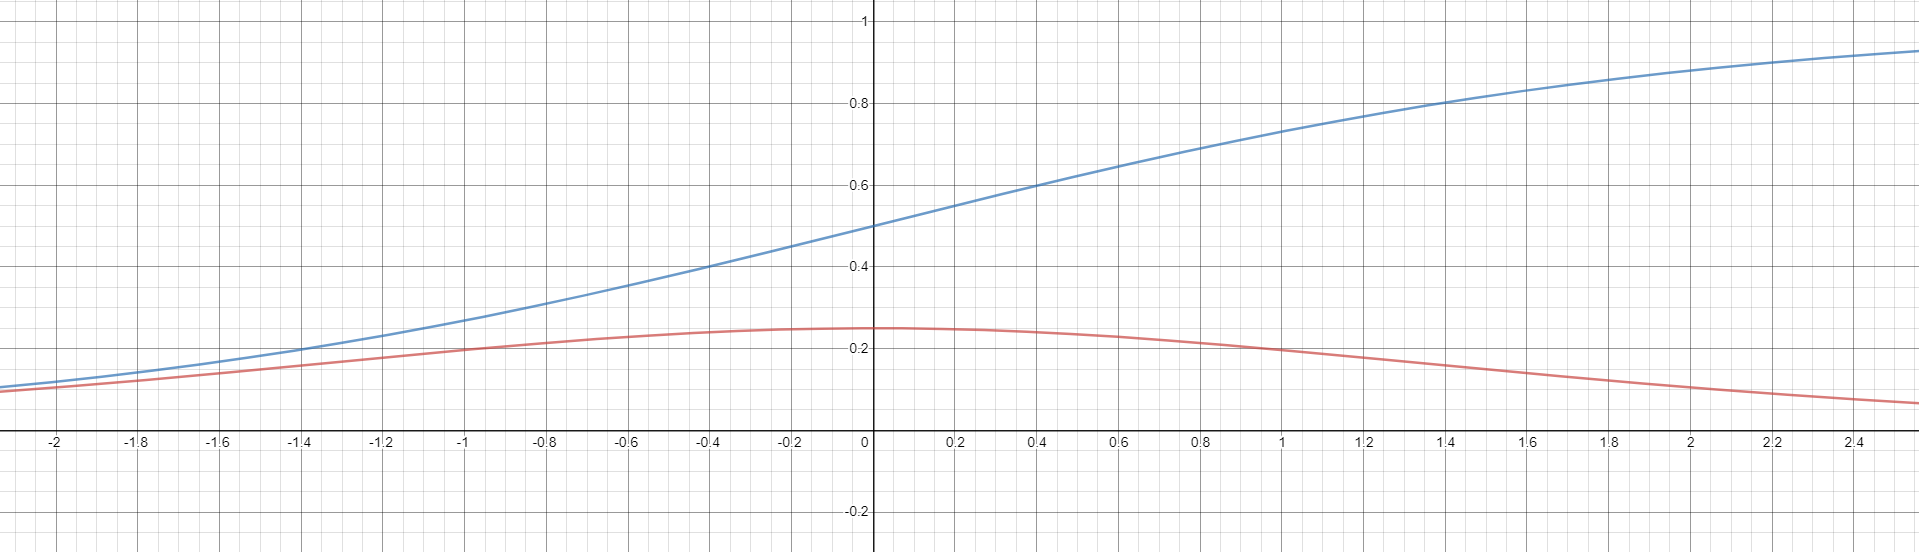
\includegraphics[width=0.75\columnwidth]{chapter03/figure/VanishingGradient.png}
        \caption{Giá trị và đạo hàm của hàm sigmoid.}
        \label{fig:VanishingGradient}
		\centering
    \end{figure}
    
    Trên hình \ref{fig:VanishingGradient}, đường màu xanh thể hiện cho giá trị của hàm sigmoid và đường màu đỏ thể hiện cho giá trị của đạo hàm. Có thể nhận ra được, với những giá trị $x$ rất lớn hoặc rất nhỏ, kết quả đạo hàm của hàm sigmoid rất gần với 0. Điều này gây ra sự triệt tiêu gradient và hạn chế khả năng học của mạng. Cụ thể, nếu mạng được khởi động bằng những trọng số quá lớn hoặc quá nhỏ, giá trị đầu vào của hàm sigmoid bị bão hòa, giá trị của đạo hàm sẽ là một giá trị gần 0 và gradient sẽ bị triệt tiêu. Nếu mạng được khởi động bằng những trọng số "đẹp" (không quá lớn, không quá nhỏ), giá trị của đạo hàm cũng sẽ là một giá trị trong khoảng (0,0.25). Khi đi qua một mạng nhiều tầng, đạo hàm của các trọng số sẽ nhỏ dần và gradient vẫn sẽ bị triệt tiêu.
    \item \textbf{Hàm sigmoid không có tính chất \textit{zero-centered}}
    \begin{figure}[!h]
	\centering
		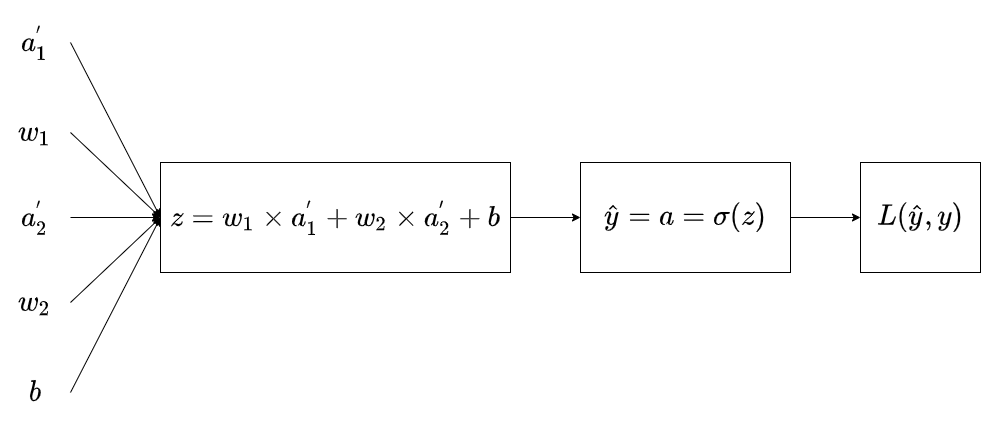
\includegraphics[width=0.5\columnwidth]{chapter03/figure/ZeroCentered.png}
        \caption{Một tầng ẩn của mạng neural nhiều lớp dùng hàm sigmoid.}
        \label{fig:ZeroCentered}
		\centering
    \end{figure}
    
    Ở ví dụ của mạng neuron như Hình \ref{fig:ZeroCentered}, đạo hàm riêng phần của hàm mất mát theo hai trọng số $w_1$ và $w_2$ sẽ được tính như sau:
    \begin{align*}
        \nabla w_{1} &= \frac{\partial L}{\partial z} \times \frac{\partial z}{\partial w_1} = \frac{\partial L}{\partial z} \times a^{'}_1\\
        \nabla w_{2} &= \frac{\partial L}{\partial z} \times \frac{\partial z}{\partial w_2} = \frac{\partial L}{\partial z} \times a^{'}_2
    \end{align*}
    
    Vì $a^{'}_1$ và $a^{'}_1$ là kết quả của một hàm sigmoid trước đó, do đó luôn nhận giá trị dương và dấu của các gradient sẽ phụ thuộc vào $\frac{\partial L}{\partial z}$. Điều này có nghĩa là các gradient sẽ luôn cùng dương hoặc luôn cùng âm. Việc cập nhật trọng số sẽ chỉ xảy ra về một phía, hạn chế sự linh hoạt của mạng và gây khó khăn cho việc hội tụ.
\end{enumerate}

\subsection{Hàm tanh}
$\indent$\textbf{Công thức:}
\[tanh(x) = \frac{e^x-e^{-x}}{e^x+e^{-x}}\]
$\indent$Hàm tanh nhận vào một số thực và trả về một giá trị trong khoảng (-1,1). Trên hình \ref{fig:Tanh}, đường màu xanh thể hiện giá trị của hàm tanh và đường màu đỏ thể hiện cho giá trị đạo hàm. Dễ dàng nhận thấy rằng hàm tanh cũng gặp phải vấn đề triệt tiêu gradient như hàm sigmoid. Tuy nhiên, so với sigmoid, hàm tanh có tính chất zero-centered.
\begin{figure}[!h]
	\centering
		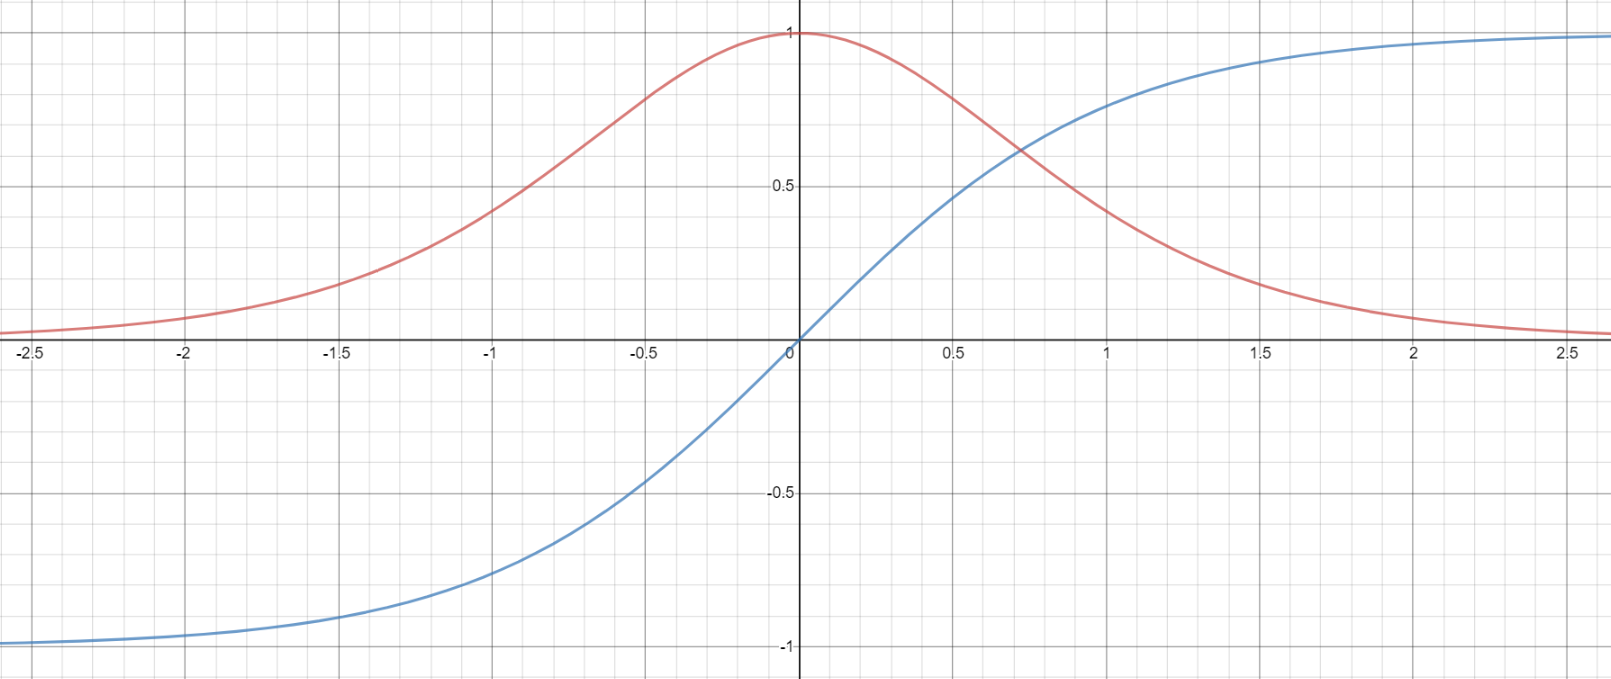
\includegraphics[width=0.75\columnwidth]{chapter03/figure/Tanh.png}
        \caption{Đồ thị và đồ thị đạo hàm của hàm tanh.}
        \label{fig:Tanh}
		\centering
\end{figure}

Hàm tanh cũng có thể được biểu diễn bằng hàm sigmoid như sau:
\[tanh(x) = 2\sigma(2x) - 1\]

\subsection{Hàm ReLU}
$\indent$\textbf{Công thức:}
\[f(x) = max(0,x)\]
\begin{figure}[!h]
	\centering
		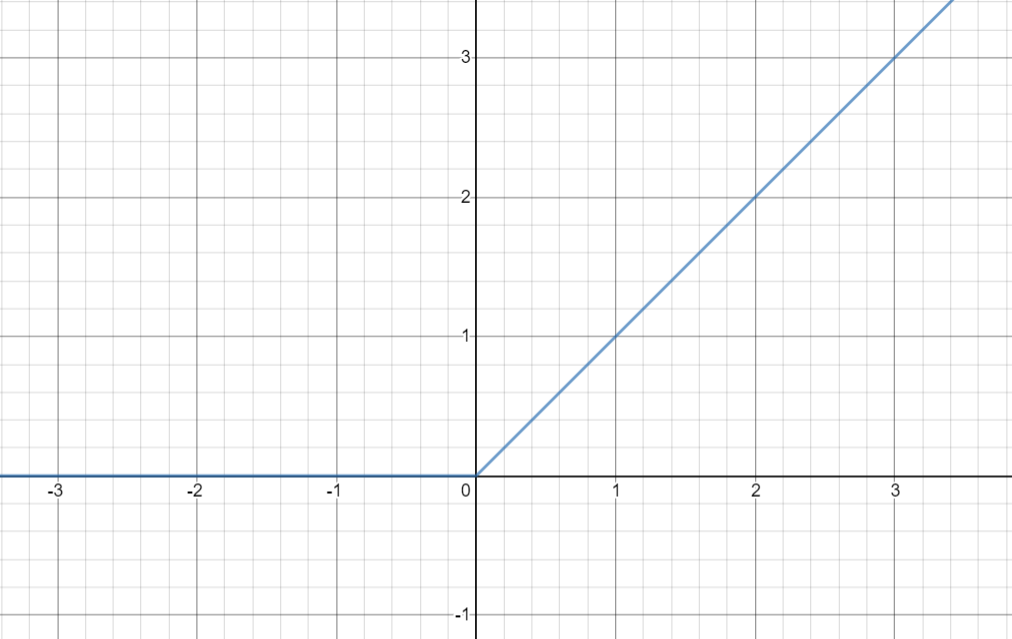
\includegraphics[width=0.75\columnwidth]{chapter03/figure/ReLU.png}
        \caption{Đồ thị của hàm ReLU.}
        \label{fig:ReLU}
		\centering
\end{figure}

Quan sát công thức và hình \ref{fig:ReLU}, dễ dàng nhận ra cách hoạt động của hàm ReLU là lọc ra các giá trị đầu vào nhỏ hơn 0. Đạo hàm của ReLU sẽ như sau:
\begin{equation}
    f'(x) = 
    \begin{cases}
      1 & \text{if } x > 0\\
      0 & \text{else}
    \end{cases}
\end{equation}

Như vậy, so với sigmoid và tanh, hàm ReLU sẽ không xuất hiện vấn đề triệt tiêu gradient. Tốc độ tính toán của hàm ReLU cũng sẽ nhanh hơn so với hai hàm trước đó. Tuy nhiên ReLU cũng tồn đọng một nhược điểm, với $x$ có giá trị nhỏ hơn 0, qua hàm  ReLU sẽ thu được kết quả bằng 0. Nếu giá trị của node bị chuyển thành 0 thì sẽ không có ý nghĩa ở lớp tiếp theo và các hệ số tương ứng từ node đấy cũng không được cập nhật với gradient. Hiện tượng này gọi là \textit{Dying ReLU}.

\subsection{Hàm leaky ReLU}
$\indent$\textbf{Công thức:} 
\[f(x) = max (0.01x,x)\]
$\indent$Leaky ReLU là một cố gắng trong việc loại bỏ Dying ReLU. Thay vì luôn trả về giá trị bằng 0 cho các giá trị âm, leaky ReLU tạo một đường xiên có độ dốc nhỏ như hình \ref{fig:leakyReLU}.
\begin{figure}[!h]
	\centering
		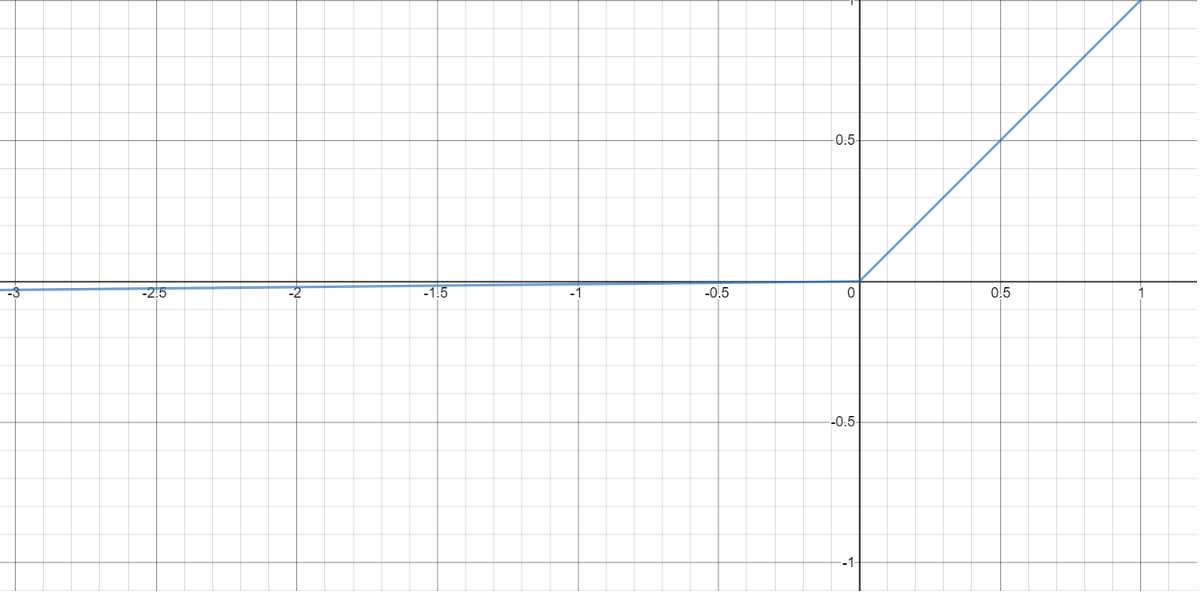
\includegraphics[width=0.75\columnwidth]{chapter03/figure/leakyReLU.png}
        \caption{Đồ thị của hàm leaky ReLU.}
        \label{fig:leakyReLU}
		\centering
\end{figure}

Leaky ReLU cũng có một biến thể khác là PReLU: $f(x) = max(\alpha x,x)$ với $\alpha$ sẽ được chọn trong quá trình học.
%%%%%%%%%%%%%%%%%%%%%%%%%%%%%%%%%%%%%%%%%%%%%%%%%

\section{Biểu diễn Neural Network như là vector và ma trận}
Chúng ta đã có những khái niệm về neural network qua những phần trước. Tuy nhiên, làm sao để máy tính có được bộ não với những neuron như vậy thì phần này sẽ đi giải đáp những vấn đề  đó.

\subsection{Làm sao biểu diễn được neural network}
Chúng ta xem xét mạng neural network gồm 3 layer như sau: 
\begin{figure}[!h]
	\centering
		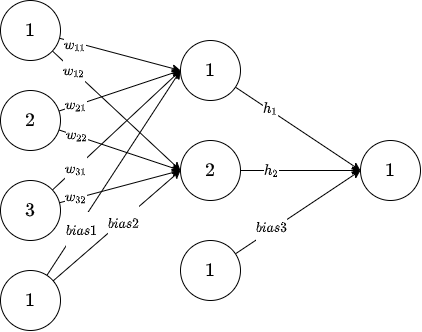
\includegraphics[width=0.5\columnwidth]{chapter03/figure/weight(1).png}
        \caption{Mạng neural network gồm 3 layer.}
        \label{fig:weight}
		\centering
\end{figure}

Dựa theo hình trên, với $f$ là hàm activation chúng ta sẽ thấy rằng:
\begin{center}
$h_{1} = f(in_{1}*w_{11}+in_{2}*w_{21}+in_{3}*w_{31}+bias_{1})$\\
$h_{2} = f(in_{1}*w_{12}+in_{2}*w_{22}+in_{3}*w_{32}+bias_{2})$\\
$out = f(h_{1}*w_{11}+h_{2}*w_{21}+bias_{3})$\\
\end{center}

Bằng một cách suy nghĩ đơn giản, chúng ta có thể lưu các giá trị $w_{i}$ vào một mảng hay một vector và duyệt tuần tự. Nhưng chúng ta nên sống chậm lại để để ý rằng, với mỗi perceptron nó sẽ được tính bằng cách lấy giá trị đầu ra của layers trước đó hoặc là giá trị input ban đầu (gọi chung là input) nhân với trọng số của nó nối với input hay nói theo kí hiệu toán học sẽ như sau:
\begin{center}
    $h_{i} = f(\sum_{j=1}^{num\_input} in_{j}*w_{ji}+bias_{i})$ (1)
\end{center}

Trong đó, $num\_input$ chính là số lượng input để tính toán trong tầng hiện tại. Nếu ai đã quen với việc tính toán ma trận thì sẽ thấy công thức này giống như việc nhân 2 ma trận với nhau.

Thật vậy, mỗi đầu ra của một perceptron là một con số (scalar) và mối quan hệ giữa 2 tầng liên tiếp là như nhau nên ở đây không mất tình tổng quát chúng ta chỉ xét riêng trường hợp với 2 tầng (nhìn hình minh họa).
\begin{figure}[!h]
	\centering
		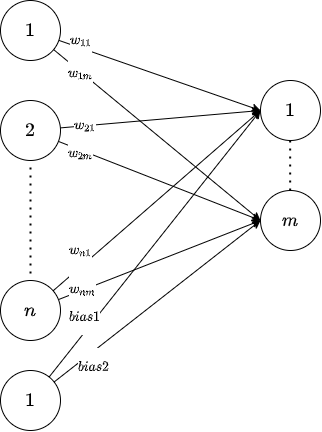
\includegraphics[width=0.5\columnwidth]{chapter03/figure/FC.png}
        \caption{Hai layer liên tiếp nhau.}
        \label{fig:FC}
		\centering
\end{figure}

Với hình trên, nếu chúng ta biểu diễn input thành 1 vector hay nói cách khác là một ma trận $X_{nx1}$. Ta sẽ xây dựng ma trận trọng số $W$ tương ứng với n hàng, m cột với $w_{ij}$ là trọng số từ input $i$ nối với một output $j$.

Dựa theo công thức ở (1), chúng ta có thể thấy rằng chỉ cần lấy cột thứ $i$ ra làm vector để nhân với vector trong ma trận cột $X$ và áp dụng activation thì ta sẽ có kết quả của perceptron thứ $i$. Do đó, việc còn lại để tính nhanh đó là ta chuyển vị ma trận trọng số $W_{nxm}$ thì sẽ trở về môn Đại số tuyến tính thân quen. Nếu lúc này chúng ta xét $h_{mx1}$ là ma trận của các perceptron đầu ra thì ta sẽ có công thức như sau:
\begin{center}
    $h = f(W^{T}*X+b)$
\end{center}

Cách biểu diễn neural network dưới dạng ma trận như thế này rất hữu ích trong việc tính toán khi thực hiện các phép lan truyền xuôi và lan truyền ngược.

\subsection{Cách biểu diễn lan truyền xuôi và lan truyền ngược}
\subsubsection{Lan truyền xuôi }
Lan truyền xuôi là quá trình tính toán thông qua các tầng ẩn mà dữ liệu đầu vào được cho ra kết quả trong mô hình. Ta kí hiệu mỗi tầng $i$ trong mạng được cấu tạo từ 3 phần đó là input $X^{(i)}$, ma trận trọng số $W^{(i)}$ và hàm activation $f^{(i)}$ , trong đó, output của tầng này sẽ là input của tầng tiếp theo. Xem xét hình minh họa dưới đây cho quá trình lan truyền xuôi.
\clearpage
\begin{figure}[!h]
	\centering
		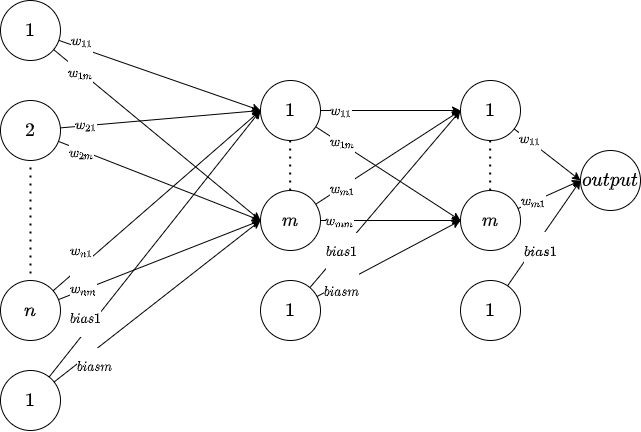
\includegraphics[width=0.75\columnwidth]{chapter03/figure/ltx.png}
        \caption{Lan truyền xuôi}
        \label{fig:ltx}
		\centering
\end{figure}

Như chúng ta thấy trong hình mạng gồm 4 layers (1 input layer, 2 hidden layer và 1 output layer).
\begin{center}
    $X^{(1)} = f^{(1)}(W^{(1)T}*Input+b^{(1)})$\\
    $X^{(2)} = f^{(2)}(W^{(2)T}*X^{(1)}+b^{(2)})$\\
    $Output = f^{(3)}(W^{(3)T}*X^{(2)}+b^{(3)})$\\
\end{center}

Với cách tính này, thì chúng ta có thể mở rộng một cách tông quát với 1 input layer, n hidden layer và 1 output layer như sau:
\begin{center}
    $X^{(1)} = f^{(1)}(W^{(1)T}*Input+b^{(1)})$\\
    $X^{(i)} = f^{(i)}(W^{(i)T}*X^{(i-1)}+b^{(i)})$, $i=\overline{2,n}$\\
    $Output = f^{(n)}(W^{(n)T}*X^{(n)}+b^{(n+1)})$\\
\end{center}

Nhìn chung, vấn đề lan truyền xuôi cũng không quá phức tạp khi đã có đại số tuyến tính can thiệp vào.

\subsubsection{Lan truyền ngược}
Lan truyền ngược là quá trình cập nhật lại cái trọng số để tìm ra bộ trọng số phù hợp để làm mô hình cho bài toán cần giải quyết. Khác với lan truyền xuôi khi sử dụng hàm activation, lan truyền ngược dựa trên việc tính đạo hàm để cho ra kết quả.

Để cập nhật được trọng số, thì chúng ta cần có hàm loss giả sử được định nghĩa là $J$ và để dễ cho quá trình tính toán, chúng ta sẽ kí hiệu thêm biểu thức sau:
\begin{center}
    $z^{(i)}=W^{(i)T}*X^{(i)}+b^{(i)}$
    $a^{(i)} = f(z^{(i)})$
\end{center}

Các kí hiệu này được biểu diễn như hình sau. Để đỡ rối khi nhìn, xin phép chỉ kí hiệu tượng trưng các đường cần thiết, thực tế sẽ mỗi perceptron ở layer trước phải nối hết với các perceptron layer sau.
\begin{figure}[!h]
	\centering
		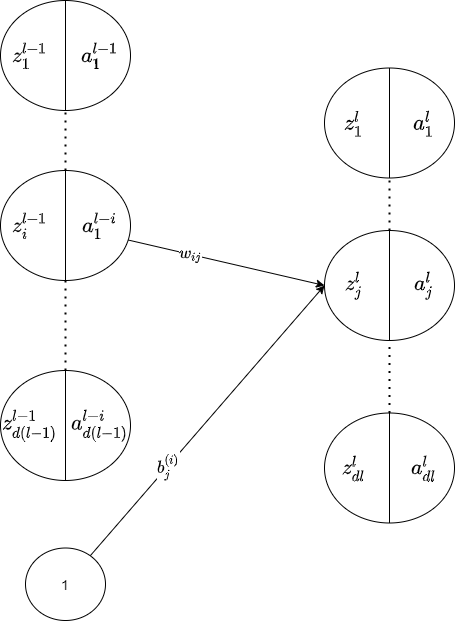
\includegraphics[width=0.5\columnwidth]{chapter03/figure/ltn.png}
        \caption{Đồ thị minh họa lan truyền ngược.}
        \label{fig:ltn}
		\centering
\end{figure}

Tiếp theo, chúng ta sẽ có được gradient của các trọng số ở từng layer l như sau:
\begin{center}
        $\frac{\partial J}{\partial w^{(l)}_{ij}} = \frac{\partial J}{\partial z_{j}^{(l)}} * \frac{\partial z_{j}^{(l)}}{\partial w^{(l)}_{ij}}=e^{(l)}_{j} * a_{i}^{(l-1)}$\\
\end{center}

với
\begin{center}
        $e^{(l)}_{j} = \frac{\partial J}{\partial z_{j}^{(l)}}=\frac{\partial J}{\partial a_{j}^{(l)}}*\frac{\partial a_{j}^{(l)}}{\partial z_{j}^{(l)}}$\\
        $=(\sum_{k=1}^{d^{(l+1)}} \frac{\partial J}{\partial z_{k}^{(l+1)}}*\frac{\partial z_{j}^{(l)}}{\partial a_{j}^{(l)}})f'(z^{(l)}_{j})$\\
        $=(w^{(l+1)}_{j:}*e^{(l+1)})f'(z^{(l)}_{j})$
\end{center}

Trong đó $e^{(l+1)} = [e_{1}^{(l+1)},e_{2}^{(l+1)},...,e_{d(l+1)}^{(l+1)}]^{T}$ và $w_{j:}^{(l+1)}$ là toàn bộ phần tử hàng thứ $j$ của ma trận $W^{(l+1)}$. Tổng xuất hiện trong công thức trên thể hiện việc $a_{j}^{(l)}$ đóng góp vào việc tính các $z_{k}^{(l+1)}$.
Với cách làm tương tự, ta có:
\begin{center}
        $\frac{\partial J}{\partial b^{(l)}_{j}} =e^{(l)}_{j}$\\
\end{center}

Từ đây chúng ta có thể mở rộng ra cho cách biểu diễn bằng ma trận như các công thức sau:
\begin{center}
    $\frac{\partial J}{\partial W^{(l)}} = a^{(l-1)}e^{(l)T}$\\
    $e^{(l-1)} = W^{(l)T}e^{(l)}f'(z^{(l)})$\\
    $\frac{\partial J}{\partial b^{(l)}} = e^{(l)}$
\end{center}

\subsection{Vì sao lại biểu diễn bằng ma trận}
Để giải quyết cho câu hỏi này, hãy thử hiện thực các tính toán trong mạng neural mà không dùng đến ma trận:
\begin{lstlisting}
    J = 0
    for i = 1 to m:
        z[i] = b
        for j in range(len(w)):
            z[i] += w[j]*x[i][j] 
        a[i] = Sigmoid(z[i])
        J += -[y[i]*log(a[i]) + (1-y[i])*log(1-y[i])]
        dz[i] = a[i] - y[i]
        for j in range(len(w)):
            dw[j] += x[i][j]*dz[i]
    J = J / m
    for j in range(len(w)):
        w[j] = w[j] - alpha*dw[j]/m
\end{lstlisting}

Và hiện thực các tính toán có sử dụng ma trận:
\begin{lstlisting}
    import numpy as np 
    
    Z = np.dot(w.T,X) + b
    A = Sigmoid(Z) #1
    dZ = A - Y
    dW = (1/m) * X * dZ.T
    dB = (1/m) * np.sum(dZ)
    W = W - alpha * dW
    b = b - alpha * dB
\end{lstlisting}

Có thể thấy, việc hỗ trợ tính toán bằng ma trận giúp ích rất nhiều trong quá trình hiện thực. Đó cũng là lý do tại sao những ngôn ngữ có hỗ trợ tính toán ma trận như Python được sử dụng phổ biến trong hiện thực mạng neural. Một lưu ý nữa được rút ra từ ví dụ trên là các nút ở cùng một tầng thì phải có cùng một hàm activation để việc áp dụng hàm activation (dòng 1) cũng ma trận hóa và trở nên dễ dàng hơn.

\subsection{Kỉ nguyên mới của neural network} 
Sau khi đã đi qua những lý thuyết của neural network thì chúng ta đã thấy được sức mạnh của phương pháp này. Tuy nhiên, đã có thời gian neural network không được sử dụng nhiều và chìm trong màn đêm. Vấn đề nằm ở chỗ, việc tính toán ma trận quá sức phức tạp và Central Processing Unit(CPU) và cả Graphics Processing Unit(GPU) thời bấy giờ chưa thể đảm nhận được công việc này. Tuy nhiên, sau khi phần cứng phát triển vượt bậc thì đã mở ra kỉ nguyên mới cho neural network.

Ngày nay, khi nhắc đến việc huấn luyện mạng neural network, người ta thường nghĩ ngay đến việc huấn luyện trên GPU. Nhưng tại sao CPU và GPU đã phát triển nhưng GPU lại chiếm ưu thế hơn trong việc lựa chọn để huấn luyện?

Để trả lời câu hỏi này, chúng ta quay lại việc lan truyền xuôi và lan truyền ngược sử dụng ma trận. Có thể nói rằng việc biểu diễn neural network bằng ma trận là cách tốt nhất trong hiện tại. Do đó, phần cứng nào có thể lưu trữ những con số dưới dạng ma trận đều có thể đảm nhận được nhiệm vụ tính toán và biểu diễn neural network tốt nhất.

Nói đến đây, ắt hẳn chúng ta đã biết tại sao GPU đã có sức ảnh hưởng mạnh mẽ đến neural network. GPU được dùng để biểu diễn hình học đồ họa máy tính, mà đồ họa máy tính được cấu thành từ ma trận pixel nên việc xử lý này không khác gì xử lý ma trận trong neural network cả. Thêm vào đó, GPU ngày nay lại được xử lý đa luồng và tiếp nhận thông tin gấp nhiều lần CPU. Hãy tưởng tượng xem, để xử lý ma trận thì CPU phải duyệt qua các phần tử trong ma trận và thực hiện tính toán, chúng ta có thể lấy CPU nhiều core nhưng chắc chắn rằng cũng chỉ vài chục là nhiều. Trong khi đó, GPU có thê lập tức biến đổi ngay vector hay ma trận nhờ vào khả năng tính toán song song của mình. Đây cũng là lý do mà chúng ta phải dùng ma trận hóa ở phần trước để tính toán và cũng là lý do vì sao các framework về học sâu ngày nay \textbf{chỉ cho dùng 1 hàm activation cho mỗi tầng}.

\section{Kết chương}
 Qua chương này, chúng ta đã tìm hiểu và phân tích được cách thức hoạt động của mạng học sâu mà ngày nay được sử dụng ngoài thực tế. Ngoài ra, các vấn đề liên quan tới GPU và ma trận hóa cũng đã được trình bày để thấy được sự ảnh hưởng của phần cứng và sự hỗ trợ của ngôn ngữ khi chúng ta huấn luyện mạng học sâu để từ đó chúng ta có phương pháp lựa chọn phần cứng, ngôn ngữ và thiết kế mô hình mạng hợp lý để tối ưu năng suất nhất có thể.

\newpage
\section{Bài tập}
\begin{exer}
Cho mạng neural network như hình vẽ sau:
%%%%%%%%%%%%Chen hinh
\begin{figure}[!h]
	\centering
		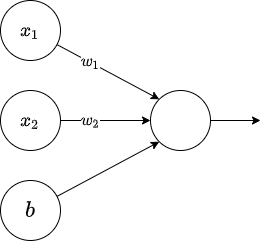
\includegraphics[width=0.5\columnwidth]{chapter03/figure/bai1.png}
        \caption{Mạng neural network một output.}
		\centering
\end{figure}\\
Biết rằng $w_{1} = w_{2} = w_{bias} = 0.25$, $x1=0.1, x2=0.2, bias= 1$ và output mong đợi là 1. Hãy tính output của mạng và các trọng số và bias mới(với hệ số học alpha là 0.1 và hàm lỗi là $CrossEntropy$) của mạng với các activation sau:
\begin{enumerate}
    \item Hàm activation là hàm $tanh$.
    \item Hàm activation là hàm $ReLU$.
\end{enumerate}
\end{exer}

\clearpage
\begin{exer}
Cho mạng neural network như hình vẽ sau:
%%%%%%%%%%%%Chen hinh
\begin{figure}[!h]
	\centering
		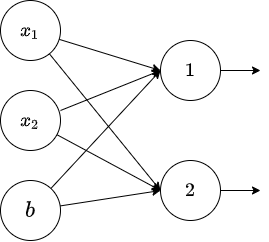
\includegraphics[width=0.5\columnwidth]{chapter03/figure/bai2.png}
        \caption{Mạng neural network hai output.}
        \label{sec3:bai2}
		\centering
\end{figure}

Biết rằng các trọng số và bias đều bằng $0.5$, $x1=0.1, x2=0.2$ và output 1, 2 mong đợi lần lượt là 0, 1. Hãy tính output của mạng và các trọng số và bias mới(với hệ số học alpha là 0.1 và hàm lỗi là $CrossEntropy$) của mạng với các activation sau:
\begin{enumerate}
    \item Hàm activation của output 1, 2 lần lượt là là hàm $tanh$, $ReLU$.
    \item Hàm activation output 1, 2 lần lượt là là hàm $tanh$, $tanh$.
\end{enumerate}
\end{exer}

\clearpage
\begin{exer}
Cho mạng neural network như hình vẽ sau:
%%%%%%%%%%%%Chen hinh
\begin{figure}[!h]
	\centering
		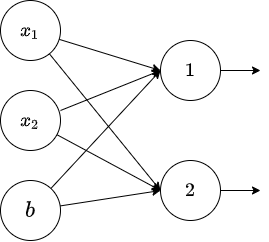
\includegraphics[width=0.5\columnwidth]{chapter03/figure/bai2.png}
        \caption{Mạng neural network hai output.}
		\centering
\end{figure}

Biết rằng các trọng số và bias đều bằng $0.5$, $x1=0.1, x2=0.2$ và output 1, 2 mong đợi lần lượt là 0, 1. Hãy dựa theo kiến thức của chương này, tìm ra các ma trận được tạo ra và dùng vectorize để tính toán thực hiện lan truyền xuôi.
\end{exer}
%classical NLP & Mô hình xử lý ngôn ngữ tự nhiên bằng mạng học sâu
\chapter{Mô hình xử lý ngôn ngữ tự nhiên bằng mạng học sâu}
\label{chp:04}
% \chapter{Phương pháp xử lý ngôn ngữ tự nhiên}
\section{Giới thiệu về xử lý ngôn ngữ tự nhiên}
\label{sec:introduction_nlp}
Xử lý ngôn ngữ tự nhiên (Natural Language Processing - NLP) là một nhánh của trí tuệ nhân tạo tập trung vào các ứng dụng trên ngôn ngữ của con người. Trong trí tuệ nhân tạo thì xử lý ngôn ngữ tự nhiên là một trong những phần khó nhất vì nó liên quan đến việc phải hiểu ý nghĩa ngôn ngữ-công cụ hoàn hảo nhất của tư duy và giao tiếp.

NLP có thể được hiểu ngắn gọn là khả năng xử lý ngôn ngữ của con người (thường được khái quát là tự nhiên), vì ngôn ngữ con người được sử dụng trong hình ảnh, viết, nói,... Từ \emph{xử lý} (process) trong từ "Xử lý ngôn ngữ tự nhiên" có nghĩa là: "Thay đổi một cái gì đó thành một thứ khác". Trong trường hợp này có nghĩa là "Lấy từ ngôn ngữ của con người và biến thành các biểu diễn mà máy tính có thể hiểu và xử lý". Ví dụ: Những từ mà bạn đang đọc và viết dưới dạng ngôn ngữ tự nhiên (tiếng Việt bằng các ký tự latin) và được lưu trong ngôn ngữ máy tính (dạng nhị phân gồm các chuỗi số gồm 0 và 1). Tuy nhiên, NLP không phải chỉ là chuyển các ký tự trong bảng chữ cái thành các bit. Nó liên quan nhiều hơn đến việc làm cho máy tính có thể hiểu, xử lý một cách tự động (hoặc làm một số tác vụ liên quan đến ngôn ngữ) dựa trên cách ngôn ngữ của con người được biểu diễn và tổ chức [\ref{refer:7}].

NLP thường liên quan đến những việc sau:
\begin{itemize}
    \item Những từ nào trong cụm từ là danh từ?
    \item Danh từ nào trong cụm từ đóng vai trò chính trong cụm từ gốc?
    \item Cụm từ này thể hiện cảm xúc gì?
    \item Từ này trong ngữ cảnh này có thể hiểu là gì?
    \item và nhiều tác vụ khác
\end{itemize}

Các ứng dụng sử dụng NLP gồm có:
\begin{itemize}
    \item \emph{Phân tích cảm xúc} (Sentiment Analysis - SA): Những đoạn văn bản có thể mang trong nó các sắc thái hoàn cảnh và có thể rất phức tạp. Ví dụ như bạn của bạn đang buồn hay tức giận, bạn sẽ có những cách hỏi chuyện khác nhau. Hay việc sử dụng từ hoặc dấu câu theo ngữ cảnh khác nhau sẽ dẫn đến những cách hiểu khác nhau. Cảm xúc có thể nhận ra từ sự kết hợp của giọng điệu, sự lựa chọn từ ngữ và phong cách viết. SA được dùng để hiễu sâu sắc hơn về ngữ cảnh của văn bản. Ví dụ như: việc đánh giá cảm xúc thích hay không thích về một sản phẩm tiểu dùng dựa trên hàng ngàn bình luận trên mạng xã hội có thể giúp cải thiện chiến dịch truyền thông của sản phẩm đó. Hay bạn có thể đánh giá dự báo thị trường chứng khoáng thông qua đánh giá mức độ lạc quan của hàng ngàn người trên một diễn đàn tài chính để giúp hỗ trợ đầu tự. Hoặc những chính trị gia có thể đánh giá phản ứng của hàng trăm ngàn người với mỗi nội dung của các chính trị gia đưa trên Twitter, Facebook.
    \item \emph{Phân loại văn bản} (Text Classification - TC): Đây có thể được coi là một trong những ứng dụng phổ biến nhất của NLP. Trong TC, các từ (nghĩa, mối quan hệ các từ, ngữ cảnh) được sử dụng như là các đặc tính để dùng cho các thuật toán xác định văn bản thuộc về lớp X, Y hay Z. Ví dụ: Google sử dụng giải thuật TC để phân loại thư điện tử gửi đến có phải là thư rác hay không.
    \item \emph{Nhận diện chủ thể} (Entity Recognition - ER): Xác định và nhận diện thông tin chính (chủ thể) trong văn bản. Một chủ thể có thể là một từ hoặc một chuỗi từ mà liên tục đề cập đến cùng một thứ. Mỗi chủ thể sẽ được xác định và đưa vào các thể loại định trước. Ví dụ như xác định từ "Microsoft" trong văn bản và phân loại nó thành mục "Công ty"[\ref{refer:8}]. 
    \item \emph{Nhận diện chủ đề} (Topic Modeling - TM): Trong NLP, thuật ngữ "chủ đề" có nghĩa là tập các từ ngữ "đi cùng với nhau". Những từ ngữ này ta sẽ gợi nhớ ra khi nghĩ đến chủ đề cụ thể. Ví dụ như chủ đề "thể thao" thì sẽ gợi nhớ ra các từ như: bóng đá, sân vận động, chạy bộ, bơi lội,... [\ref{refer:9}].
    \item \emph{Dịch máy} (Machine Translation): NLP có thể giúp phiên dịch tự động văn bản từ ngôn ngữ này sang một ngôn ngữ khác. Có nhiều thách thức đối với dịch máy bao gồm như: sự đa dạng về ngôn ngữ, bảng chữ cái và ngữ pháp, khó khăn khi xác định việc phiên dịch có chính xác hay không [\ref{refer:10}].
    % \item \emph{Nhận diện giọng nói} (Speech Recognition)
    \item \emph{Trả lời tin nhắn tự động} (Chatbot): với sự hỗ trợ của NLP, chatbot có thể dễ dàng hiểu được câu hỏi của khách hàng với những từ ngữ tự nhiên hơn mà khong cần sự hỗ trợ từ con người.
    \item \emph{Tự động tóm tắt văn bản (Automatic Summarization)}: Tóm tắt văn bản là nhiệm vụ cô đọng một đoạn văn bản thành phiên bản ngắn hơn, giảm kích thước của văn bản ban đầu đồng thời bảo tồn các yếu tố thông tin chính và ý nghĩa của nội dung. Vì tóm tắt văn bản thủ công là một công việc tốn kém thời gian và thường tốn nhiều công sức, việc tự động hóa tác vụ này đang ngày càng phổ biến và do đó tạo thành động lực mạnh mẽ cho nghiên cứu học thuật.
    \item và các ứng dụng khác.
\end{itemize}

\subsection{Mô hình xử lý ngôn ngữ tự nhiên cổ điển}
\label{sec:classic_nlp}
Theo phương pháp cổ điển, các tác vụ xử lý ngôn ngữ tự nhiên gồm có 2 bước chính như sau:
\begin{itemize}
    \item Tiền xử lý (Pre-processing)
    \item Mô hình hóa (Modeling)
\end{itemize}

Hình \ref{fig:pipeline-nlp-classic} mô tả mô hình xử lý ngôn ngữ tự nhiên cổ điển. Thông qua 2 bước pre-processcing và modeling ta sẽ nhận được output mong muốn như là: Phân tích cảm xúc, Phân loại văn bản,...

\begin{figure}[h!]
\begin{center}
	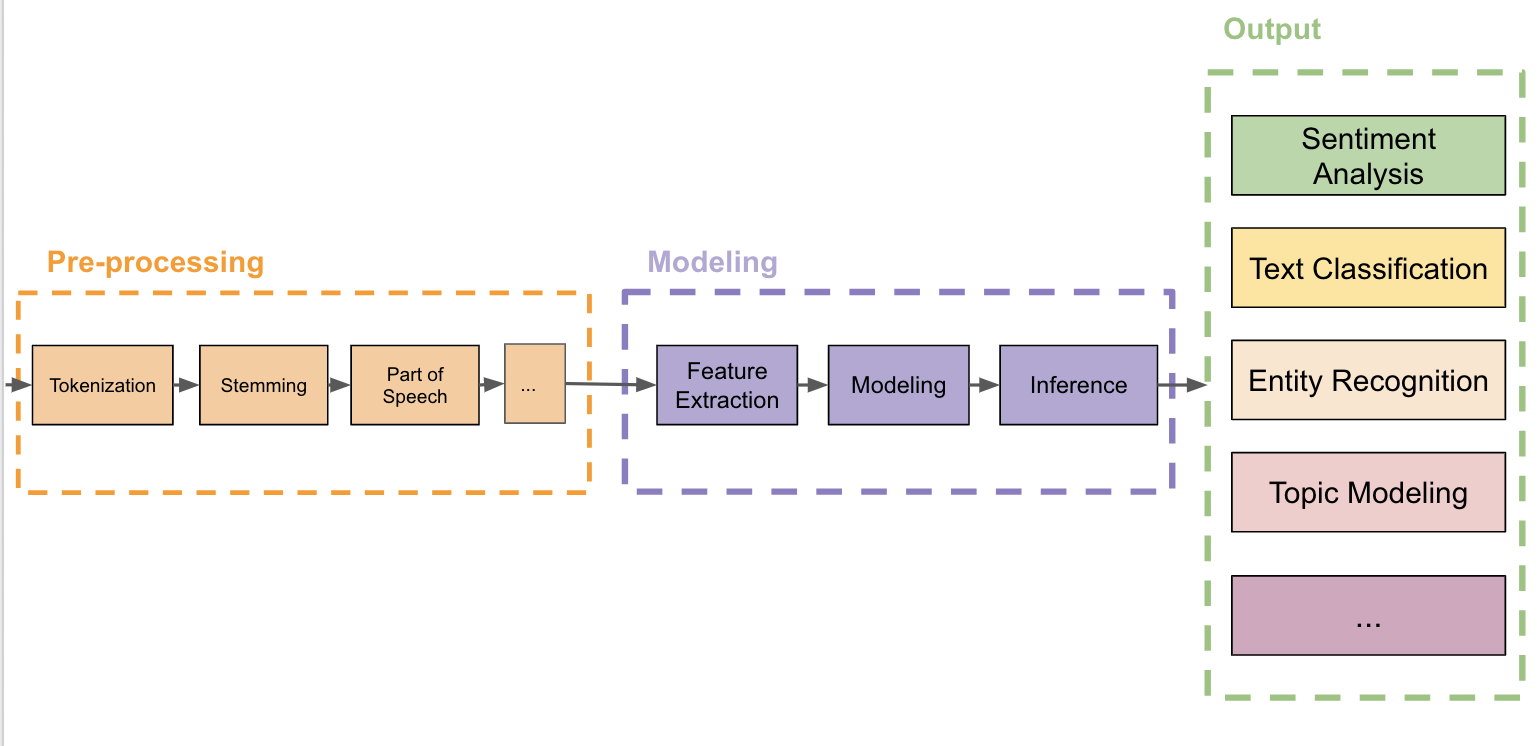
\includegraphics[width=1.0\textwidth]{chapter04/figure/classic_nlp.png}
	\caption{Pipeline cho xử lý ngôn ngữ tự nhiên theo hướng cổ điển}
	\label{fig:pipeline-nlp-classic}
\end{center}
\end{figure}

\subsection{Tiền xử lý}
\label{preprocessing}
Tiền xử lý (Preprocessing): đây là một điều quen thuộc đối với Khoa học dữ liệu (Data Science - DS). Đối với dữ liệu số, thông thường ta sẽ áp dụng mộ số quy tắt chuẩn hóa (nhằm giảm sự khác biệt giữa giá trị lớn nhất và nhỏ nhất), thay thế các giá trị không phải là dạng số (cũng như là các giá trị rỗng), phát hiện các giá trị ngoại lệ,...

Bởi vì từ và cụm từ phức tạp hơn các số nguyên và số thực, dữ liệu cần được qua vài bước tiền xử lý hay còn gọi là luồn tiền xử lý (Preprocessing Pipeline - PPL). 

\begin{figure}[h!]
\begin{center}
	\includegraphics[width=1.0\textwidth]{chapter04/figure/pre_processing.png}
	\caption{Luồng tiền xử lý}
	\label{fig:nlp-classic}
\end{center}
\end{figure}

Các bước của Preprocessing thường tùy thuộc vào từng dự án và mục đích. Hình \ref{fig:nlp-classic} mô tả các bước thông dụng trong tiền xử lý. Chi tiết các bước gồm có:
\begin{itemize}
    \item Tiền xử lý chuỗi thô (Bare String Preprocessing): được coi là một trong những bước chính của tiền xử lý. Đây là hành động sử dụng các hàm cụ thể của ngôn ngữ lập trình để sửa đổi dữ liệu đầu vào (như thay thế ký tự, tìm và thay thế các mẫu tự).
    \item Tách từ (Tokenization): là quá trình chuyển một dãy các ký tự thành một dãy các token (token là một dãy các ký tự mang ý nghĩa cụ thể, biểu thị cho một đơn vị ngữ nghĩa trong xử lý ngôn ngữ). Nhiều khi token được hiểu là một từ mặc dù cách hiểu này không hoàn toàn chính xác. Ví dụ như trong tiếng Anh các từ thường được phân tách bằng dấu cách, tuy nhiên từ New York vẫn chỉ được coi là một từ mặc dù nó có dấu cách ở giữa. Do đó chỉ có 1 token trong trường hợp này. Một ví dụ khác là I’m được coi là 2 từ ‘I’ và ‘am’ mặc dù không có dấu cách nào. Trong trường hợp này ta có 2 token. Một điểm cần lưu ý ở đây là chúng ta cần phân biệt khái niệm ‘word type’ và ‘word token’. Types là tổng số các từ có mặt trong một corpus, không tính số lần xuất hiện của từ đó (dù một từ có xuất hiện 40 lần trong đoạn dữ liệu thì cũng chỉ được tính là 1). Trong khi đó, Token tính cả tổng số lần xuất hiện của từng từ. Ví dụ trong câu ‘a good person is a person who is willing to help others’ có tất cả 9 Types (do có 9 từ xuất hiện) nhưng có tới 12 Tokens (do từ ‘a’, ‘person’ và ‘is’ đều xuất hiện 2 lần). 
    \item Biến đổi từ về dạng gốc (Stemming): đây là kỹ thuật dùng để biến đổi 1 từ về dạng gốc (được gọi là stem hoặc root form) bằng cách cực kỳ đơn giản là loại bỏ 1 số ký tự nằm ở cuối từ mà nó nghĩ rằng là biến thể của từ. Ví dụ như chúng ta thấy các từ như walked, walking, walks chỉ khác nhau là ở những ký tự cuối cùng, bằng cách bỏ đi các hậu tố -ed, -ing hoặc -s, chúng ta sẽ được từ nguyên gốc là walk.
    \item Phân loại từ trong câu (Part of Speech - POS): POS là việc phân loại các từ trong một câu (danh từ, trạng từ, tính từ hay động từ,...). Việc phân loại từ như thế này sẽ góp phần nắm được thêm ý nghĩa của câu thay vì chỉ xem nó như là tập hợp của các ký tự. Ví dụ như cùng là một từ “can” nhưng nó có thể có nghĩa là “có thể” hoặc nghĩa là “cái lon“, như vậy POS có thể giúp máy tính phân biệt được điều này một cách dễ dàng tùy vào nội dung của câu.
    \item Từ vựng hóa (Lemmatization): Làm trở lại nguyên dạng ban đầu các từ vựng bị biến đổi thể (inflection) hoặc được kết hợp (conjugatetion). Ví dụ như: biến đổi từ ate -> eat.
    \item Loại bỏ các từ dừng (Stop word Removal): Stop word là những từ xuất hiện nhiều trong ngôn ngữ tự nhiên, tuy nhiên lại không mang nhiều ý nghĩa. Trong tiếng Việt, stop word là những từ như: để, này, kia... Tiếng Anh là những từ như: is, that, this... Mục đích của tác vụ này là loại bỏ những từ không mang lại nhiều ý nghĩa cho mô hình.
\end{itemize}

\subsection{Mô hình hóa}
Sau khi thực hiện bứơc tiền xử lý, ta sẽ thực hiện mô hình hóa. Mô hình hóa gồm các bước như sau để thu được output.

\begin{itemize}
    \item Rút trích đặt trưng (Extract features): Để sử dụng được các giải thuật Machine learning, ta cần vector hóa dữ liệu đầu vào. Bước này sẽ giúp ta thực hiện được điều đó.
    \item Xây dựng mô hình (Modelling): dựa vào mục đích ta sẽ xây dựng mô hình, mô hình sẽ còn tuỳ thuộc vào giải thuật Machine learning cụ thể.
    \item Inference: dùng mô hình xây dựng được để áp dụng vào các tác vụ cụ thể.
\end{itemize}

\section{Trích xuất đặc trưng - Feature Extraction}
Trong bước Modeling, trích xuất đặc trưng là một vấn đề khá quan trọng để rút trích các features để đưa vào các model ML.

Dưới đây là 2 phương pháp cơ bản để trích xuất feature:
\begin{itemize}
    \item Vector hóa bằng kỹ thuật đếm (Count-Vectorization - (Bag-of-words) - BOW)
    \item TF-IDF (Term Frequency, Inverse Term Frequency.)
\end{itemize}

\subsection{Phương pháp Bag of words}
Một trong những cách tốt để chuyển các  token thành các feature, cũng là phương pháp mang ý tưởng cốt lõi cho các phương pháp chuyển các  token thành các feature về sau là kỹ thuật BOW. Hướng tiếp cận này rất đơn giản và linh hoạt

Trong phương pháp này, ta sẽ dựa trên những token để tìm tần suất xuất hiện của mỗi token.

Cùng xem ví dụ về 3 câu sau:
\begin{enumerate}
    \item "Hôm qua tôi đi học"
    \item "Hôm nay tôi cũng đi học"
    \item "Ngày mai tôi không đi học"
\end{enumerate}
Thông qua bước tokenization ta biến đổi được thành các câu:
\begin{enumerate}
    \item "Hôm\_qua tôi đi học"
    \item "Hôm\_nay tôi cũng đi học"
    \item "Ngày\_mai tôi không đi học"
\end{enumerate}

Qua bước này "hôm qua", "hôm nay", "ngày mai" được biến đổi thành từ "hôm\_qua", "hôm\_nay", "ngày\_mai".

Ta sẽ xem mỗi câu là một văn bản riêng biệt và ta xây dựng một danh sách tất cả các từ từ 3 câu trên. Ta sẽ được các từ như sau: 
\begin{itemize}
    \item Hôm\_qua
    \item Hôm\_nay
    \item Ngày\_mai
    \item tôi
    \item cũng
    \item không
    \item đi
    \item học
\end{itemize}

Bước tiếp theo ta sẽ xây dựng vector. Vector sẽ chuyển các văn bản thành input cho các giải thuật học máy.

Với câu đầu tiên "Hôm\_qua tôi đi học", dựa vào tần suất xuất hiện từ(các từ này là duy nhất trong tập) trong câu ta xây dựng được vector như sau:
\begin{itemize}
   \item 'Hôm\_qua'= 1
    \item 'Hôm\_nay' = 0
    \item 'Ngày\_mai' = 0
    \item 'tôi' = 1
    \item 'cũng' = 0
    \item 'không' = 0
    \item 'đi' = 1
    \item 'học' = 1
\end{itemize}

=> [1, 0, 0, 1, 0, 0, 1, 1]

Các câu còn lại ta sinh được vector như sau:
\begin{itemize}
    \item Hôm\_nay tôi cũng đi học => [0, 1, 0, 1, 1, 0, 1, 1]
    \item Ngày\_mai tôi không đi học => [0, 0, 1, 1, 0, 1, 1, 1]
\end{itemize}

Dưới đây là ma trận ta thu được từ phương pháp BOW (Bảng \ref{tab:bow_vector}):

\begin{table}[h!]
\centering
\begin{tabular}{|l|l|l|l|l|l|l|l|l|}
\hline
Câu & Hôm\_qua & Hôm\_nay   & Ngày\_mai & tôi    & cũng   & không   & đi   & học \\ \hline
Câu 1     & 1     & 0 & 0  & 1    & 0    & 0 & 1 & 1 \\ \hline
Câu 2     & 0     & 1    & 0  & 1 & 1 & 0    & 1    & 1    \\ \hline
Câu 3     & 0     & 0 & 1     & 1 & 0 & 1    & 1    & 1   \\ \hline
\end{tabular}
\caption{Bảng ma trận vector thu được từ phương pháp BOW}
\label{tab:bow_vector}
\end{table}
% \newpage

% Tuy nhiên với phương pháp này, nó tồn tại một số vấn đề bất lợi:

% Đầu tiên là thứ tự các token không được giữ nguyên, điều này ảnh hưởng đến ngữ nghĩa của câu. Đó là lý do tại sao ta gọi là BOW bởi Bag là không mang ý nghĩa thứ tự.

% Thứ hai, bộ đếm không được chuẩn hóa giữa các document với nhau.

\subsection{Phương pháp TF-IDF}

% Thực tế, cách tốt nhất để duy trì các token là việc quan tâm đến các cặp token, bộ ba các token liên tiếp hoặc nhiều hơn thế nữa thay vì chỉ quan tâm đến token riêng lẻ. Cách tiếp cận này được gọi là Extracting-N-Grams. Ví dụ như 1-gram tương ứng với 1 token, 2-gram tuong ứng 2 token, n-gram tương ứng n token.

% Ví dụ sau sẽ minh họa cho bigrams ( 2 cặp token):
% Ta có câu sau "Cause she doesn't get your humor like I do.". Bigrams từ câu này gồm có:

% \begin{itemize}
%     \item 'cause she'
%     \item 'she doesn't'
%     \item 'doesn't get'
%     \item 'get your'
%     \item 'your humor'
%     \item 'humor like'
%     \item 'like I'
%     \item 'I do'
% \end{itemize}

% \begin{figure}[h!]
% \begin{center}
% 	\includegraphics[width=0.25\textwidth]{chapter04/figure/example.png}
% 	\caption{Ví dụ minh họa TF-IDF}
% 	\label{fig:nlp-classic}
% \end{center}
% \end{figure}

% Với cùng 3 ví dụ ở mục trước, bây giờ các cột ko phải chỉ là 1 token riêng biệt mà bây giờ là một cặp token. Và các câu review cũng được chuyển sang dạng vector một cách tương ứng với phương pháp Bag of words, với giá trị 1 / 0 thể hiện cho việc cặp token có xuất hiện / ko xuất hiện trong câu review tương ứng hay không.

% Hãy để ý ở đây, cách biểu diễn ở mức này mới chỉ đưa ra được mối quan hệ thứ tự cục bộ (local) trong câu, nhưng cái mà ta mong muốn là phân tích đoạn text đầu vào một cách tốt hơn. Và một vấn đề nữa đó là sẽ có rất nhiều các feature mà ta sẽ có ở đây nếu lấy một cặp các token. Giả sử số lượng token lên đến 100000 token thì số lượng các features có thể tăng lên theo cấp số mũ.

% Để giải quyết vấn đề này, ta sẽ loại bỏ một số n-grams dựa trên tần suất xuất hiện của chúng trong tập hợp các câu review đầu vào của ta (corpus). Có ba trường hợp gồm:
% \begin{itemize}
%     \item n-grams có tần suất xuất hiện cao
%     \item n-grams có tần suất xuất hiện thấp
%     \item n-grams có tần suất xuất hiện trung bình
% \end{itemize}


% n-grams có tần suất xuất hiện cao: trường hợp này xuất hiện trong hầu hết các văn bản, bạn đều có thể thấy được n-grams này. Ví dụ với Tiếng Anh, đó có thể là các giới từ (a, an, this, that, v.v... ). Và bởi vì ta chỉ sử dụng cấu trúc ngữ pháp, cho nên chúng không có ý nghĩa nhiều lắm. Chúng được gọi với cái tên là stop words, nó không thực sự giúp ta phân biệt các đoạn text với nhau, nên các từ này này cần được loại bỏ.

% n-grams có tần suất xuất hiện thấp: trường hợp này đến từ lỗi gõ sai từ người dùng, hoặc là thường hiếm xuất hiện trong bất kỳ các văn bản nào trong tập dữ liệu của  ta. Các trường hợp này cũng cần nên loại bỏ vì nó sẽ gây ra overfit cho model.

% n-grams có tần suất xuất hiện trung bình: đây là các n-grams tốt nhất bởi vì chúng bao gồm n-grams mà không có 2 trường hợp nêu trên. Vấn đề là trong tập n-grams có tấn suất xuất hiện trung bình, có rất nhiều n-grams thuộc các dải tần số xuất hiện khác nhau. Thật hữu ích khi chúng hữu dụng để có thể dựa vào tần số mà có thể lọc được n-grams là tốt, n-grams nào là xấu hơn. Nếu  ta có thể ranking các n-grams này theo mức độ quan trọng của chúng thì sẽ ra sao, chắc chắn sẽ rất có lợi. Chúng ta có thể quyết định được n-grams với tần suất xuất hiện trung bình thì n-grams nào là tốt, n-grams nào là xấu. Và ý tưởng ở đây là : n-grams có tần suất nhỏ hơn sẽ được đánh trọng số cao hơn vì nó là thể hiện cho các trường hợp riêng biệt trong câu review.



TF-IDF là từ viết tắt của thuật ngữ tiếng Anh "term frequency – inverse document frequency", TF-IDF là trọng số của một từ trong văn bản thu được qua thống kê thể hiện mức độ quan trọng của từ này trong một văn bản, mà bản thân văn bản đang xét nằm trong một tập hợp các văn bản. TF-IDF khắc phục được nhược điểm của BOW.

Ví dụ ta có một câu như sau:

"Today is a beautiful day"
  
Bạn nghĩ gì khi đọc câu này? Từ gì bạn tập trung nhiều hơn. Câu này nói về hôm nay (today), nó cũng nói là hôm nay là ngày đẹp trời (today is a beautiful day), cảm xúc trong câu này là tích cực, vui vẻ. Đẹp (beauty) rõ ràng là tính từ được sử dụng ở đây. Với phương pháp BOW, tất cả các từ đều có cùng số lần xuất hiện (tần suất) như nhau (1 trong trường hợp này) và rõ ràng các từ đều được coi ngang hàng nhau (tầm quan trọng như nhau (và không nhấn mạnh được từ cần nhấn mạnh trong câu (từ beauty).

Một trường hợp khác, trong một tài liệu có 200 từ, từ 'a', 'the' xuất hiện rất nhiều lần (20 lần từ 'a', 15 lần từ 'the'). Những từ này xuất hiện nhiều lần không có nghĩa là chúng quan trọng. BOW cũng không giải quyết được vấn đề này.

Ưu điểm:
\begin{itemize}
    \item Dễ tính toán
    \item Đây là cách đon giản để trích xuất các mô tả trong văn bản
    \item Dễ dàng tính toán sự giống nhau giữa 2 văn bản
\end{itemize}

Nhược điểm:
\begin{itemize}
    \item TF-IDF dựa trên BOW nên vì thế nó không thể thể hiện tầm quan trọng của vị trí từ trong văn bản, ngữ nghĩa, sự tương quan giữa các từ trong các văn bản khác nhau
\end{itemize}

TF-IDF gồm 2 trọng số TF và IDF.

TF - Term Frequency : dùng để ước lượng tần xuất xuất hiện của từ trong văn bản. Tuy nhiên với mỗi văn bản thì có độ dài khác nhau, vì thế số lần xuất hiện của từ có thể nhiều hơn. Vì vậy số lần xuất hiện của từ sẽ được chia độ dài của văn bản (tổng số từ trong văn bản đó)

\begin{center}
    $TF(t, d) =  \frac{( \text{số lần từ t xuất hiện trong văn bản d})}{ (\text{tổng số từ trong văn bản d})}$
\end{center}

IDF - Inverse Document Frequency: dùng để ước lượng mức độ quan trọng của từ đó như thế nào . Khi tính tần số xuất hiện TF thì các từ đều được coi là quan trọng như nhau. Tuy nhiên có một số từ thường được được sử dụng nhiều nhưng không quan trọng để thể hiện ý nghĩa của đoạn văn, ví dụ:
\begin{itemize}
    \item Từ nối: và, nhưng, tuy nhiên, vì thế, vì vậy,...
    \item Giới từ: ở, trong, trên,...
    \item Từ chỉ định: ấy, đó, nhỉ,...
\end{itemize}

Vì vậy ta cần giảm đi mức độ quan trọng của những từ đó bằng cách sử dụng IDF

\begin{center}
    \(IDF(t, D) = log(\frac{\text{Tổng số văn bản trong tập mẫu D}}{\text{Số văn bản có chứa từ t}})\)
\end{center}

Từ đó ta có công thức TF-IDF

\begin{center}
    \(TFIDF(t, d, D) = TF(t, d) x IDF(t, D)\)
\end{center}

Mỗi tài liệu sẽ được biểu diễn bằng một vector tf.idf, vector này sẽ số chiều là K với K độ dài tất cả các từ có trong tất cả các văn bản của tập dữ liệu.

Ví dụ về TF-IDF:

Dữ liệu ban đầu ta có 3 văn bản như sau:
\begin{itemize}
    \item Document 1: "Hôm\_qua tôi đi học"
    \item Document 2: "Hôm\_nay tôi cũng đi học"
    \item Document 3: "Ngày\_mai tôi không đi học"
\end{itemize}

Đầu tiên ta sẽ xây dựng bảng từ vựng trong corpus. Bảng \ref{tab:sec3exmptfidf} là bảng ta thu được khi xây dựng bảng từ vựng.
\begin{table}[h!]
\centering
\begin{tabular}{|l|l|lll}
\cline{1-2}
Word  & Count &  &  &  \\ \cline{1-2}
Hôm\_qua & 1     &  &  &  \\ \cline{1-2}
Hôm\_nay    & 1     &  &  &  \\ \cline{1-2}
Ngày\_mai & 1     &  &  &  \\ \cline{1-2}
tôi & 3     &  &  &  \\ \cline{1-2}
cũng & 1     &  &  &  \\ \cline{1-2}
không & 1     &  &  &  \\ \cline{1-2}
đi & 3     &  &  &  \\ \cline{1-2}
học & 3     &  &  &  \\ \cline{1-2}
\end{tabular}
\caption{Bảng từ vừng trong corpus}
\label{tab:sec3exmptfidf}
\end{table}

Tiếp theo ta sẽ tính TF cho mỗi từ ứng với mỗi văn bản trong corpus. Bảng \ref{tab:sec3caltf} là kết quả tính giá trị TF cho mỗi từ vựng ứng với mỗi văn bản.

\begin{table}[h!]
\centering
\begin{tabular}{|l|l|l|l|l}
\cline{1-4}
Words/Document & Document 1 & Document 2 & Document 3 &  \\ \cline{1-4}
Hôm\_qua          & 0.25       & 0       & 0       &  \\ \cline{1-4}
Hôm\_nay          & 0       & 0.2          & 0       &  \\ \cline{1-4}
Ngày\_mai          & 0       & 0       & 0.2          &  \\ \cline{1-4}
tôi              & 0.25          & 0.2       & 0.2       &  \\ \cline{1-4}
cũng             & 0          & 0.2       &  0      &  \\ \cline{1-4}
không             & 0       & 0          & 0.2          &  \\ \cline{1-4}
đi             & 0.25       & 0.2          & 0.2          &  \\ \cline{1-4}
học           & 0.25       & 0.2          & 0.2          &  \\ \cline{1-4}
\end{tabular}
\caption{Bảng tính TF cho các tài liệu}
\label{tab:sec3caltf}
\end{table}

Bước kế tiếp ta cần tính giá trọ IDF cho mỗi từ vựng. Bảng \ref{tab:sec3calidf} liệt kê kết quả tính IDF cho mỗi từ vựng.

\begin{table}[h!]
\centering
\begin{tabular}{|l|l|l}
\cline{1-2}
Words & IDF value &  \\ \cline{1-2}
Hôm\_qua & log(3/1) = 0.48 &  \\ \cline{1-2}
Hôm\_nay    & log(3/1) = 0.48 &  \\ \cline{1-2}
Ngày\_mai & log(3/1) = 0.48 &  \\ \cline{1-2}
tôi     & log(3/3) = 0  &  \\ \cline{1-2}
cũng    & log(3/1) = 0.48 &  \\ \cline{1-2}
không    & log(3/1) = 0.48 &  \\ \cline{1-2}
đi    & log(3/3) = 0 &  \\ \cline{1-2}
học  & log(3/3) = 0 &  \\ \cline{1-2}
\end{tabular}
\caption{Bảng tính IDF cho các văn bản}
\label{tab:sec3calidf}
\end{table}

Cuối cùng ta dựa vào giá trị TF và IDF ta sẽ tính được vector TF-IDF cho mỗi từ vựng dựa theo công thức \(TF-IDF = TF . IDF\). Bảng \ref{tab:sec3caltfidf} mô tả ma trận kết quả thu được. 

\begin{table}[h!]
\centering
\begin{tabular}{|l|l|l|l|l|l|l|l|l|}
\hline
  & Hôm\_qua & Hôm\_nay & Ngày\_mai & tôi    & cũng   & không   & đi  & học \\ \hline
Document 1     & 0.12     & 0 & 0  & 0    & 0    & 0 & 0 & 0 \\ \hline
Document 2     & 0     & 0.1    & 0  & 0 & 0.1 & 0    & 0    & 0    \\ \hline
Document 3     & 0     & 0 & 0.1     & 0 & 0 & 0.1    & 0    & 0    \\ \hline
\end{tabular}
\caption{Bảng tính TF-IDF}
\label{tab:sec3caltfidf}
\end{table}
\newpage

Sau khi tính TF-IDF, mỗi document đã được vector hóa bằng phương pháp này (số chiều của vector chính là số từ ta trong tất cả document, số chiều = 8) gồm:

\begin{itemize}
    \item "Hôm\_qua tôi đi học" =>  [0,12, 0, 0,0, 0, 0, 0, 0]
    \item  "Hôm\_nay tôi cũng đi học" => [0, 0.1, 0, 0, 0.1, 0, 0, 0]
    \item "Ngày\_mai tôi không đi học" [0, 0, 0.1, 0, 0, 0.1, 0, 0]
\end{itemize}

Dựa vào công thức TF-IDF ta cũng nhận ra một hạn chế của $TF_IDF$ này là không biểu diễn được quan hệ giữa các từ trong văn bản.

Ví dụ như câu: "Đi học hôm\_qua tôi" thông qua TF-IDF cũng ra vector [0,12, 0, 0,0, 0, 0, 0, 0] tương tự câu "Hôm\_qua tôi đi học".

\section{Mô hình xử lý ngôn ngữ tự nhiên bằng mạng học sâu}
Hướng tiếp cận cổ điển của việc xử lý ngôn ngữ tự nhiên (NLP - Natural Language Processing, hình \ref{fig:pipeline-nlp-classic}) đã sử dụng trong nhiều năm trước về căn bản đã có thể thay thế bằng mô hình Deep Learning (gọi tắt là DL). Hình \ref{fig:deep-learning-based-nlp} là một mô hình đơn giản được đưa ra nhằm mục đích để  cố gắng đạt được những kết quả mong đợi như phương pháp tiếp cận cổ điển đã đem đến nhưng với hướng tiếp cận hiện đại - sử dụng mô hình học sâu. Hiện nay, đã có rất nhiều mô hình DL cùng các kĩ thuật phức tạp được đề ra nhằm để giải quyết các bài toán khác nhau, nhưng về căn bản thì mọi thứ đã được thể hiện thông qua hình \ref{fig:deep-learning-based-nlp}.

\begin{figure}[h!]
\begin{center}
	\includegraphics[width=1.0\textwidth]{chapter04/figure/nlp-deep-model.png}
	\caption{Mô hình Deep Learning sử dụng cho NLP}
	\label{fig:deep-learning-based-nlp}
\end{center}
\end{figure}

Dựa vào đó, ta có thể thấy rằng, để xây dựng mô hình NLP dựa trên Deep Learning thì ta cần phải trải qua một số bước:
\begin{itemize}
    \item Cũng như mô hình cổ điển, dữ liệu được dùng để huấn luyện cũng cần phải trải qua bước tiền xử lý như tokenization, biến đổi từ về dạng gốc, từ vựng hóa, loại bỏ các từ vựng...
    \item Sau đó, do mạng Deep Learning chỉ tương tác trên các ma trận, vector và con số nên sẽ cần có một bước để chuyển các từ này thành các vector. Đó chính là mục tiêu chính của Embedding Layer.
    \item Và liền kề theo đó thì bước Modeling của mô hình cổ điển cũng sẽ được thay thế bằng kiến trúc hiện đại hơn - Neural Network. Và Output của Neural Network này sẽ được sử dụng phù hợp đối với từng công việc khác nhau như Sentiment, Classification, Topic Modeling...
\end{itemize}

Như vậy khi ta áp dụng mô hình vào một bài toán nhất định, ta có thể thấy là một cách rất tự nhiên rằng sau khi huấn luyện kết thúc, mạng Deep Learning có thể tự động học, sau đó đã rút trích được các đặc trưng cần thiết và biến đổi chúng thành các trọng số  ở các Hidden Layers. Đây cũng chính là lý do giải thích cho ta thấy được rằng kiến trúc mạng Deep Neural Network có thể được sử dụng để thay thế cho mô hình xử lý ngôn ngữ tự nhiên cổ điển.

Quay lại với Embeddings Layer, có rất nhiều cách để có thể biến đổi dữ liệu đầu vào thành các vector. Với 3 tài liệu ở ví dụ đầu tiên đã nêu ra, ta sẽ có một tập từ điển có 8 từ được sắp xếp theo bảng chữ cái. Thì một trong những cách biến đổi là mỗi tài liệu ứng với 1 vector 1 x 8 (do có 8 từ), giá trị của các phần tử trong vector này chính là số lần xuất hiện của từ đó trong tài liệu. Ví dụ, với tài liệu là "Hôm\_qua tôi đi học" sẽ tương đương với vector là [0 1 1 0 1 0 0 1].

Tuy nhiên, nhờ vào sức mạnh tính toán của mạng học sâu, ta vẫn có cách biểu điễn để giúp cho tập tài liệu của ta thể hiện nhiều thông tin hơn. Cụ thể hơn là thay vì biểu diễn cả tài liệu chỉ thông qua một vector thì ta sẽ biểu diễn từng từ trong tài liệu thành từng vector. Điều này có nghĩa với cách tiếp cận này, sau khi ta áp dung cho tập tài liệu "Hôm\_qua tôi đi học" thì ta sẽ tạo ra được một ma trận 4 x 8 (do có 4 từ, mỗi từ được thể hiện bằng một vector có kích thước là 8).

Quá trình biến đổi từ thành các vector này còn được biết đến với một cái tên khác là Word Embedding. Trong mục \ref{sec:word-embedding-in-details}, ta sẽ tìm hiểu kĩ hơn về các kĩ thuật được sử dụng cho Word Embedding một cách chi tiết để sử dụng chúng hiệu quả hơn.

% Biểu diễn từ thành vector bằng kỹ thuật word embedding
\section{Các kỹ thuật Word Embedding}
\label{sec:word-embedding-in-details}
Hầu hết những giải thuật Machine Learning, đặc biệt là những giải thuật sử dụng mạng nơ-ron như MLP, Deep Learning không làm việc hiểu quả trên dữ liệu văn bản. Word Embedding là một trong những là kĩ thuật được sử dụng trong xử lý ngôn ngữ tự nhiên nhằm số hoá một từ ở dạng văn bản mà con người hiểu, sang dạng cho phép máy tính có thể tính toán và xử lý được. 

Word embedding được sử dụng rộng rãi và phổ biến trong những dự án xử lý ngôn ngữ tự nhiên không chỉ vì khả năng biểu diễn văn bản dưới dạng số, mà kĩ thuật này còn cho phép nhúng (embedding) ngữ nghĩa của từ trong văn bản vào định dạng số mà máy tính có thể hiểu và xử lý hiệu quả.

Từ khi khái niệm word embedding ra đời, đã có rất nhiều giải thuật được trình bày như word2vec, GolVe, ELMO, BERT, v.v. Tuy nhiên một giải thuật Word embedding cần phải thoả mãn 2 yêu cầu dưới đây:

\begin{itemize}
    \item Tồn tại một và chỉ một cách biểu diễn cho một từ. Nghĩa là hai từ khác nhau sẽ được số hoá thành hai dạng biểu diễn khác nhau.
    
    \item Hai từ có ngữ nghĩa tương tự nhau, khoảng cách cũng sẽ gần nhau sau khi được biểu diễn sang không gian mới.
\end{itemize}


\subsection{Biểu diễn từ bằng one-hot vector}
\label{one-hot-vector-in-details}

Trước khi Word embedding ra đời, kĩ thuật được sử dụng phổ biến để số hoá một từ là sử dụng one-hot vector. Kĩ thuật này được áp dụng trong các mô hình học máy cổ điển trong giai đoạn tiền xử lý, nhằm biến đổi những dữ diệu dạng categorical sang numerical. Từ đó giúp máy tính có thể tính toán và xử lý được.

One-hot vector là một vector chứa dữ liệu nhị phân (0 và 1), tuy nhiên chỉ có một chiều trong vector được kích hoạt mang giá trị 1, toàn bộ những chiều còn lại đều mang giá trị 0. One-hot encoding là kĩ thuật biểu diễn một tập các giá trị rời rạc sang một tập one-hot vector. Để hiểu rõ hơn, xem xét ví dụ dưới đây.

Danh sách nhà mạng viễn thông ở Việt Nam là một tập hợp các giá trị rời rạc bao gồm: Viettel, Mobifone, Vinaphone, Sphone, Beeline. Sử dụng kĩ thuật one-hot vector, chúng ta có thể biểu diễn giá trị Mobifone bằng một vector trong hình \ref{fig:mobifone-onthot}.

\begin{figure}[h!]
\begin{center}
	\includegraphics[width=1.0\textwidth]{chapter04/figure/mobifone-onehot.png}
	\caption{Biểu diễn Mobifone bằng one-hot vector.}
	\label{fig:mobifone-onthot}
\end{center}
\end{figure}

Vector này có 5 chiều tương đương với 5 nhà mạng chúng ta có. Trong đó tại chiều thứ 2, tương ứng với vị trí của Mobifone trong danh sách nhà mạng, mang giá trị 1, những chiều còn lại mạng giá trị không. Tự tự, chúng ta có thể biểu diễn các nhà mạng khác bằng các vector one-hot được trình bày trong bảng \ref{table:one-hot-vector-example}.

\begin{table}[h!]
    \centering
    \begin{tabular}{ |c|c|c|c|c|c| } 
    \hline
         & Viettel & Mobifone & Vinaphone & SPhone & Beeline \\
    \hline
        Viettel & 1 & 0 & 0 & 0 & 0 \\
        Mobifone & 0 & 1 & 0 & 0 & 0\\
        Vinaphone & 0 & 0 & 1 & 0 & 0\\
        SPhone & 0 & 0 & 0 & 1 & 0\\
        Beeline & 0 & 0 & 0 & 0 & 1 \\
    \hline
    \end{tabular}
    \caption{Sử dụng one-hot vector để biểu diễn các nhà mạng ở Việt Nam}
    \label{table:one-hot-vector-example}
\end{table}

Chúng ta có thể dễ dàng nhận thấy, tập hợp từ trong văn bản cũng thuộc miền giá trị rời rạc. Do đó, kĩ thuật one-hot encoding có thể sử dụng nhằm biểu diễn một từ sang dạng one-hot vector.

Xem xét các câu sau đây (sau khi tokenize):
\begin{itemize}
    \item Hôm\_qua tôi đi học
    \item Hôm\_nay tôi cũng đi học
    \item Ngày\_mai tôi không đi học
\end{itemize}

Tập từ điển của chúng ta có 8 từ: "Hôm\_qua", "Hôm\_nay", "Ngày\_mai", "Tôi", "Đi", "Học", "Cũng", "Không". 

Để biểu diễn sang dạng số, chúng ta sử dụng one-hot vector có 8 chiều. Tám tương ưng ứng với số từ trong từ điển. Mở rộng ra, khi từ điển chúng ta có n từ, chúng ta biến đổi mỗi từ sang one-hot vector có n chiều. Đa phần các chiều của vector mang giá trị 0, chỉ duy nhất ở chiều tương ứng với vị trí của từ trong từ điển được kích hoạt mạng giá trị 1. Bảng \ref{table:one-hot-vector-from-dict} thể hiện việc chuyển đổi từ sang one-hot vector.

\begin{table}[h!]
    \centering
    \begin{tabular}{ |c|c|c|c|c|c|c|c|c| } 
    \hline
         & Hôm\_qua & Hôm\_nay & Ngày\_mai & Tôi & Đi & Học & Cũng & Không \\
    \hline
        Hôm\_qua & 1 & 0 & 0 & 0 & 0 & 0 & 0 & 0 \\
        Hôm\_nay & 0 & 1 & 0 & 0 & 0 & 0 & 0 & 0\\
        Ngày\_mai & 0 & 0 & 1 & 0 & 0 & 0 & 0 & 0\\
        Tôi & 0 & 0 & 0 & 1 & 0 & 0 & 0 & 0\\
        Đi & 0 & 0 & 0 & 0 & 1 & 0 & 0 & 0\\
        Học & 0 & 0 & 0 & 0 & 0 & 1 & 0 & 0\\
        Cũng & 0 & 0 & 0 & 0 & 0 & 0 & 1 & 0\\
        Không & 0 & 0 & 0 & 0 & 0 & 0 & 0 & 1 \\
    \hline
    \end{tabular}
    \caption{Sử dụng one-hot vector để biểu diễn các từ trong từ điển.}
    \label{table:one-hot-vector-from-dict}
\end{table}

Dựa vào kĩ thuật One-hot encoding, chúng ta đã có thể biểu diễn bất kì từ nào sang dạng số mà máy tính có thể xử lý. Rất nhiều mô hình xử lý ngôn ngữ tự nhiên và học máy đã sử dụng kĩ thuật này và mang lại hiệu quả khả quan, đặc biệt khi số lượng từ trong từ điển tương đối nhỏ. Tuy kĩ thuật này đã đảm bảo được yêu cầu biểu diễn hai từ khác nhau với hai vector khác nhau, nó vẫn mang nhiều khuyết điểm cần được cải tiến:

\begin{itemize}
    \item Giới hạn khả năng tính toán của máy tính: Hầu hết các chiều của one-hot vector mang giá trị 0, và nhiều mô hình học máy không làm việc hiệu quả trên vector có số chiều lớn (high dimensional vector) và “thưa” (sparse vector).
    
    \item Overfitting khi số lượng từ trong từ điển tăng: Với kĩ thuật này, mỗi khi chúng ta gia tăng số lượng từ trong từ điển lên n, số chiều của one-hot vector cũng tăng tương ứng lên n. Bởi vì số chiều của vector tương ứng với số lượng từ ta có trong từ điển. Trong ví dụ trên chúng ta chỉ có 8 từ trong từ điển, nhưng trong thực tế số từ trong từ điển là rất lớn, có thể đến vài ngàn, chục ngàn từ. Càng nhiều từ, càng nhiều thông số (parameter) mà mô hình học máy cần phải học. Càng nhiều thông số, chúng ta lại cần càng nhiều dữ liệu huấn luyện (training dataset) để xây dựng mô hình tốt, và không bị overfitting.
    
    \item Thiếu khả năng tổng quát hoá: Qua quá trình tiến hoá của con người, ngôn ngữ được sinh ra và phát triển theo thời gian. Khi nhìn vào một từ, chúng ta không chỉ biết ý nghĩa của mỗi từ đó mà còn hiểu được sự liên kết với những từ khác, và có khả năng tổng quát hoá ý nghĩa của một nhóm các từ liên quan. Nhờ khả năng tổng quá hoá, chúng ta có thể rút ngắn thời gian học một kiến thức mới. Ví dụ, chúng ta biết được mèo biết leo cây và ăn thịt, trong khi đó hổ và báo cũng tương tự như mèo (tổng quá hoá), nhờ vậy chúng ta có thể dự đoán được hổ vào báo cũng có thể leo cây và ăn thịt.
    
    Khi xây dựng một mô hình học máy, chúng ta muốn mô hình cũng có khả năng tổng quát hoá như chúng ta nhằm rút ngắn thời gian huấn luyện. Quay lại ví dụ trên, khi mô hình đang được huấn luyện trên dữ liệu đầu vào là “mèo”, chúng ta có dữ liệu đầu vào mới là “hổ”. Nếu hiểu được “mèo” và “hổ” tương tự nhau, mô hình không cần học “hổ” từ đầu, thay vào đó mô hình có thể sử dụng lại những thông số (parameter) được huấn luyện với đầu vào là “mèo”. Từ đó rút ngắn thời gian và lượng dữ liệu để huấn luyện mô hình. 
    
    Với kĩ thuật one-hot encoding, mỗi từ được biểu diễn thành một vector riêng lẽ, và khoảng cách giữa các vector đều bằng nhau và bằng sqrt(2). Do đó, mô hình không thể sử dụng lại những “kiến thức” đã được huấn luyện cho những từ liên quan với nhau về mặt ngữ nghĩa.

\end{itemize}

\subsection{Kỹ thuật Auto-Encoder để thu giảm số chiều}
\subsubsection{Giới thiệu}

Auto-Encoder là mô hình mạng nơ-ron, được huấn luyện dựa trên cơ chế học không giám sát (unsupervised learning), nhằm biểu diễn dữ liệu đầu vào ở dạng vector nhiều chiều (high-dimensonal vector) bằng một vector có số chiều nhỏ hơn (low-demensial vector). Mô hình này được sử dụng trong kĩ thuật dữ liệu (data engineering) cho phép thu giảm số chiều của dữ liệu đầu vào, nhằm giúp trực quan hoá dữ liệu; tăng khả năng tính toán của máy tính, giảm số lượng thông số của mô hình (parameter) từ đó rút ngắn thời gian huấn luyện; v.v. 

Mô hình Auto-Encoder hoạt động dựa trên cơ chế compress và reconstruct. Theo đó, mô hình phải học cách biểu diễn dữ liệu đầu vào với một lượng thông tin ít hơn (compress), sao cho nó vẫn có thể tái tạo lại được dữ liệu đầu vào dựa trên lượng thông tin đó (reconstruct). Một cách hiểu đơn giản là mô hình hoạt động tương tự như cơ chế nén và giải nén file của WinRar. Mô hình được phân loại trong mô hình học không giám sát (unsupervised learning) bởi vì chúng ta không cần chuẩn bị nhãn (ground-truth hoặc label) để huấn luyện mô hình. Nó sử dụng chính dữ liệu đầu vào làm nhãn, vì mục đính của mô hình là học để tái tạo lại dữ liệu ban đầu.

\subsubsection{Kiến trúc mô hình Auto-Encoder}

\begin{figure}[h!]
\begin{center}
	\includegraphics[width=1.0\textwidth]{chapter04/figure/auto-encoder-architecture.png}
	\caption{Mô hình Auto-Encoder sử dụng mạng nơ-ron 3 lớp.}
	\label{fig:auto-encoder-architecture}
\end{center}
\end{figure}

Kiến trúc mô hình Auto-Encoder là một mạng nơ-ron 3 lớp như hình \ref{fig:auto-encoder-architecture}. Trong đó hidden layer có số nút nhỏ hơn rất nhiều so với số nút ở Input và Output. Auto-Encoder bao gồm các thành phần quan trọng sau:

\begin{itemize}
    \item Encoder: là một ma trận Nxk, trong đó N là số chiều của vector đầu vào, k là số nút của hidden layer. Để mô hình  học được cách biểu vector đầu vào bằng một vector có số chiều nhỏ hơn, mô hình được thiết kế với số nút ở hidden layer nhỏ hơn so với số nút ở lớp Input và Output (k << N). Ma trận làm nhiệm vụ compress dữ liệu đầu vào ở không gian nhiều chiều N (high-dimensional space) sang không gian có số chiều nhỏ hơn k (low-dimensional space). Dữ liệu đầu vào sau khi đi qua ma trận Encoder, chúng ta nhận được một vector có số chiều là k, được gọi là encoded vector.
    \item Decoder: ngược với với Encoder, Decoder là một ma trận kxN làm nhiệm vụ reconstruct dữ liệu đầu vào dựa trên encoded vector sinh ra tự bộ Encoder. Ở đây vector có số chiều là k sẽ được biến đổi để trở về vector ban đầu có số chiều là N. Đầu ra của bộ Decoder là một vector gần giống với vector đầu vào. Mô hình được huấn luyện để giảm khoảng cách giữa vector đầu vào và vector đầu ra nhất có thể. Mục tiêu này được thể hiện thông qua một hàm lỗi chính là khoảng cách Euclidean giữa vector đầu vào và vector đầu ra.
\end{itemize}

\subsubsection{Quá trình huấn luyện mô hình Auto-Encoder}
Xem xét các câu sau đây (sau khi tokenize):
\begin{itemize}
    \item Hôm\_qua tôi đi học
    \item Hôm\_nay tôi cũng đi học
    \item Ngày\_mai tôi không đi học
\end{itemize}

Tập từ điển của chúng ta có 8 từ: "Hôm\_qua", "Hôm\_nay", "Ngày\_mai", "Tôi", "Đi", "Học", "Cũng", "Không". 

Ma trận Encoder và Decoder của mô hình Auto-Ecoder trong hình \ref{fig:auto-encoder-architecture}, được khởi tạo lần lượt như sau:

Ma trận Encoder 8 x 4:
$\begin{bmatrix}
 3 & 2 & 1 & 5 \\
 4 & 5 & 7 & 8 \\
 2 & 1 & 2 & 4 \\
 4 & 2 & 1 & 2 \\
 1 & 3 & 1 & 3 \\
 2 & 4 & 2 & 1 \\
 4 & 5 & 2 & 7 \\
 6 & 4 & 4 & 5 
\end{bmatrix}$

Ma trận Decoder 4 x 8:
$\begin{bmatrix}
 4 & 5 & 1 & 2 & 5 & 1 & 5 & 6 \\
 5 & 6 & 8 & 1 & 9 & 0 & 2 & 4 \\
 3 & 2 & 1 & 4 & 2 & 5 & 7 & 9 \\
 7 & 5 & 7 & 9 & 2 & 1 & 3 & 1
\end{bmatrix}$

Để huấn luyện mô hình, chúng ta lần lượt lặp qua từng từ (token) trong tập corup. Tại mỗi step, tương ứng với một từ, vector đầu vào và output mong đợi của mô hình chính là one-hot vector của từ đó. Quá trình huấn luyện mô hình trong mỗi step chi tiết như sau (giả sử chúng ta bắt đầu với "Hôm\_qua"):
\begin{enumerate}
    \item Nhân vector one-hot của "Hôm\_qua" với ma trận Encoder kích thước 8 x 4. Sau khi nhân, chúng ta thu được một encoded vector của "Hôm\_qua". Vector này có số chiều là 4. Do tính chất đặc biệt của one-hot vector (chỉ có duy nhất một vị trí có giá trị là 1), encoded vector này cũng chính là hàng thứ 1 của ma trận Encoder, tương ứng với ví trí của "Hôm\_qua" trong từ điển. Phía dưới, mô tả quá trình khi nhân one-hot vector của "Hôm\_qua" với ma trận Encoder:
    \begin{displaymath} 
        \begin{bmatrix}
        \boldsymbol{1} & 0 & 0 & 0 & 0 & 0 & 0 & 0
        \end{bmatrix} \times
        \begin{bmatrix}
         \boldsymbol{3} & \boldsymbol{2} & \boldsymbol{1} & \boldsymbol{5} \\
         4 & 5 & 7 & 8 \\
         2 & 1 & 2 & 4 \\
         4 & 2 & 1 & 2 \\
         1 & 3 & 1 & 3 \\
         2 & 4 & 2 & 1 \\
         4 & 5 & 2 & 7 \\
         6 & 4 & 4 & 5 
        \end{bmatrix} =
        \begin{bmatrix}
        3 & 2 & 1 & 5
        \end{bmatrix}
    \end{displaymath}
    
    \item Tiếp tục nhân encoded vector với ma trận Decoder, ta thu được vector đầu ra, có số chiều bằng với vector đầu vào:
    \begin{displaymath} 
        \begin{bmatrix}
        3 & 2 & 1 & 5
        \end{bmatrix} \times
        \begin{bmatrix}
        4 & 5 & 1 & 2 & 5 & 1 & 5 & 6 \\
        5 & 6 & 8 & 1 & 9 & 0 & 2 & 4 \\
        3 & 2 & 1 & 4 & 2 & 5 & 7 & 9 \\
        7 & 5 & 7 & 9 & 2 & 1 & 3 & 1
        \end{bmatrix} =
        \begin{bmatrix}
        60 & 54 & 55 & 57 & 45 & 13 & 41 & 40
        \end{bmatrix}
    \end{displaymath}
    
    \item Loss của mô hình là khoảng cách Euclidean giữa vector one-hot của "Hôm\_qua" với vector đầu ra:
    \begin{displaymath}
        Loss = \sqrt{(1-60)^2 + (0-54)^2 + ... + (0-41)^2 + (0-40)^2} \approx 134.71
    \end{displaymath}
    
    \item Sử dụng kĩ thuật Back-propagation, mô hình điều chỉnh thông số của hai ma trận Encoder và Decoder qua mỗi step.
\end{enumerate}

Tương tự như vậy, chúng ta tiếp tục lặp qua các từ còn lại trong corpus. Trong những bước huấn luyện đầu, vector đầu ra từ Decoder sẽ khác với vector đầu vào, do độ lỗi mô hình lúc này khá lớn. Tuy nhiên, sau quá trình huấn luyện lặp đi lặp lại trên tập corpus, mô hình sẽ hội tụ. Lúc này vector đầu ra sẽ không giống nhưng xấp xỉ với vector one-hot đầu vào.

Ví dụ, sau quá trình huấn luyện:

Ứng với vector one-hot đầu vào của từ "Hôm\_nay"
\begin{center}
$\begin{bmatrix}
0 & 1 & 0 & 0 & 0 & 0 & 0 & 0
\end{bmatrix}$
\end{center}

Vector đầu ra của mô hình Auto-Encoder sẽ là
\begin{center}
$\begin{bmatrix}
0.001 & 0.99 & 0.0012 & 0.00023 & 0.0004 & 0.0011 & 0.0001 & 0.00005
\end{bmatrix}$
\end{center}

Giả sử sau khi huấn luyện xong, ma trận Encoder và Decoder lần lượt như sau:

Ma trận Encoder 8 x 4:
$\begin{bmatrix}
 0.2 & 0.1 & 0.5 & 0.2 \\
 0.6 & 0.5 & 0.3 & 0.3 \\
 0.4 & 0.2 & 0.8 & 0.9 \\
 0.1 & 0.7 & 0.5 & 0.3 \\
 0.8 & 0.4 & 0.9 & 0.1 \\
 0.5 & 0.1 & 0.1 & 0.3 \\
 0.1 & 0.6 & 0.1 & 0.7 \\
 0.3 & 0.2 & 0.4 & 0.5
\end{bmatrix}$

Ma trận Decoder 4 x 8:
$\begin{bmatrix}
 0.3 & 0.3 & 0.6 & 0.1 & 0.7 & 0.7 & 0.3 & 0.8 \\
 0.2 & 0.5 & 0.4 & 0.2 & 0.7 & 0.1 & 0.5 & 0.2 \\
 0.1 & 0.5 & 0.3 & 0.9 & 0.9 & 0.2 & 0.3 & 0.1 \\
 0.3 & 0.5 & 0.2 & 0.5 & 0.1 & 0.2 & 0.6 & 0.1
\end{bmatrix}$

Do tính chất đã đề cập trong bước một trong mỗi step khi huấn luyện mô hình, chúng ta có thể thấy rằng ma trận Encoder chứa toàn bộ encoded vector của các từ trong từ điển. Vector ở hàng thứ i chính là encoded vector của từ thứ i trong từ điển. Ví dụ, encoded vector của từ "Ngày\_mai" tương ứng với hàng thứ 3, trong ma trận Encoder là: 

$\begin{bmatrix}
0.4 & 0.2 & 0.8 & 0.9
\end{bmatrix}$.

\subsubsection{Khả năng tổng quát hoát của mô hình Auto-Encoder}

Do kiến trúc đặc biệt của mô hình Auto-Encoder và định nghĩa của hàm lỗi, mô hình bắt buộc phải học được cách biểu diễn dữ liệu đầu vào bằng một lượng thông tin ít hơn, xúc tích hơn, theo đó tổng quát hơn, nhưng vẫn phải giữ lại được ý nghĩa cốt lõi nhằm tái tạo lại dữ liệu đầu vào. Hoạt động này giống như khi ta đang tóm tắt nội dung của một văn bản gồm nhiều trang chỉ bằng một đoạn văn ngắn vậy. Để làm được điều này, chúng ta phải hiểu và giữ lại được những nội dung quan trọng, cốt lõi, trong khi loại bỏ những thông tin dư thừa. 

Nhờ vào khả năng tổng quát này của mô hình, những dữ liệu đầu vào có tính chất tương đồng với nhau (2 vector đầu vào có khoảng cách gần nhau) thì thông tin sau khi được compress cũng sẽ gần giống nhau và ngược lại. Ví dụ nếu đầu vào là "Hôm\_qua", "Hôm\_nay", và "Học"; thì khoảng cách giữa encoded vector của "Hôm\_qua" và "Hôm\_nay" sẽ gần nhau hơn, so với encoded vector của "Hôm\_qua" và "Học".

Tuy nhiên, với tính chất của việc biểu diễn từ bằng one-hot vector (khoảng cách giữa các vector luôn bằng nhau và bằng $\sqrt{2} $). Sau khi được compress bởi mô hình Auto-Encoder, khoảng cách giữa cách encoded vector cũng sẽ bằng nhau cho mọi từ. Do đó, mô hình Auto-Encoder vẫn chưa giải quyết được yêu cầu thứ hai của một giải thuật Word embedding. Chúng ta cần một kĩ thuật mạnh mẽ hơn, có thể biểu diễn được sự tương quan về mặt ngữ nghĩa giữa các từ bằng định dạng máy tính có thể hiểu được.

\subsubsection{Bài tập TF-IDF và Auto-Encoder}
\begin{exer}
\label{chp04:exer1}
Cho corpus gồm 3 tài liệu như sau:

\begin{itemize}
    \item Hay mình đi ăn bún cá
    \item Mình đi ăn phở nha
    \item Mình ăn sáng nha
\end{itemize}

Cho sẵn tập từ vựng (sau khi tokenize) từ tập corpus ở trên như sau: \(\{\text{ hay, mình, đi, ăn, bún\_cá, phở, nha, sáng }\}\)

Hãy vector hóa 3 tài liệu trên bằng phương pháp TF-IDF.
\end{exer}

\begin{exer}
Cho mô hình Auto-Encoder như hình \ref{fig:auto-encoder-architecture}. Trong đó
\begin{itemize}
    \item Tập từ điển tương tự như bài tập \ref{chp04:exer1}.
    \item Trạng thái ma trận Encoder, và Decoder lần lượt như sau:
    
    Ma trận Encoder 8 x 4:
    $\begin{bmatrix}
     0.2 & 0.1 & 0.5 & 0.2 \\
     0.6 & 0.5 & 0.3 & 0.3 \\
     0.4 & 0.2 & 0.8 & 0.9 \\
     0.1 & 0.7 & 0.5 & 0.3 \\
     0.8 & 0.4 & 0.9 & 0.1 \\
     0.5 & 0.1 & 0.1 & 0.3 \\
     0.1 & 0.6 & 0.1 & 0.7 \\
     0.3 & 0.2 & 0.4 & 0.5
    \end{bmatrix}$
    
    Ma trận Decoder 4 x 8:
    $\begin{bmatrix}
     0.3 & 0.3 & 0.6 & 0.1 & 0.7 & 0.7 & 0.3 & 0.8 \\
     0.2 & 0.5 & 0.4 & 0.2 & 0.7 & 0.1 & 0.5 & 0.2 \\
     0.1 & 0.5 & 0.3 & 0.9 & 0.9 & 0.2 & 0.3 & 0.1 \\
     0.3 & 0.5 & 0.2 & 0.5 & 0.1 & 0.2 & 0.6 & 0.1
    \end{bmatrix}$
\end{itemize}
Cho biết vector đầu ra của mô hình của khi vector đầu vào là vector one-hot của từ "Phở"?
\end{exer}

% Word2vec
\subsection{Kỹ thuật word2vec}
\textit{word2vec} là một trong những kỹ thuật được sử dụng phổ biến nhất trong lĩnh vực \textit{Xử lý ngôn ngữ tự nhiên}. \textit{word2vec} được tạo ra và công bố vào năm 2013 bởi một nhóm các nhà nghiên cứu dẫn đầu bởi Tomas Mikolov ở Google và đã được đăng ký bảo hộ quyền phát minh sáng chế.

Kỹ thuật \textit{word2vec} đã giải quyết vấn đề tương quan ngữ nghĩa của mô hình Auto-Encoder khi biến đổi các từ trong một \textit{kho ngữ liệu} (corpus) thành các vector bằng cách dựa vào \textit{thông tin ngữ cảnh} (contextual information) của chúng trong \textit{kho ngữ liệu} đó. Bởi vậy, mô hình sẽ học để sinh ra các vector tương tự nhau cho những từ có ngữ cảnh tương tự nhau.

\textit{Thông tin ngữ cảnh} của một \textit{từ mục tiêu} (focus word) là một \textit{cửa sổ} (window) chứa các từ ở bên trái và bên phải của \textit{từ mục tiêu}, được gọi là các \textit{từ ngữ cảnh} (context word). Ta nói \textit{kích thước cửa sổ} (window size) = $k$ khi \textit{cửa sổ} này chứa $k$ từ bên trái và $k$ từ bên phải của \textit{từ mục tiêu}. Ta xét một ví dụ đơn giản sau:

\begin{exmp}
\label{ex:skip-gram-corpus}
\hrulefill\\
Giả sử \textit{kho ngữ liệu} của ta gồm 3 tài liệu D1, D2, D3:

	D1: \textit{Hôm qua tôi đi học.}
	
    D2: \textit{Hôm nay tôi cũng đi học}
    
    D3: \textit{Ngày mai tôi không đi học.}
    
Sau bước tiền xử lý, \textit{kho ngữ liệu} trên sẽ được biến đổi thành tập các từ phân biệt được sắp xếp theo thứ tự bảng chữ cái như sau: \{\textit{cũng, đi, học, hôm\_nay, hôm\_qua, không, ngày\_mai, tôi}\}.

Với \textit{kích thước cửa sổ} = 1, ta có \textit{thông tin ngữ cảnh} của các từ trong tài liệu D1 như sau:

\begin{table}[!h]
\centering
\begin{tabular}{|l|l|}
\hline
\textbf{Từ mục tiêu} & \textbf{Từ ngữ cảnh} \\ \hline
hôm\_qua             & tôi                  \\ \hline
tôi                  & hôm\_qua, đi         \\ \hline
đi                   & tôi, học             \\ \hline
học                  & đi                   \\ \hline
\end{tabular}
\caption{Từ mục tiêu và ngữ cảnh tương ứng của D1 khi kích thước cửa sổ = 1}
\label{tab:window-size-1}
\end{table}

Với \textit{kích thước cửa sổ} = 2, ta có \textit{thông tin ngữ cảnh} của các từ trong tài liệu D1 như sau:

\begin{table}[ht]
\centering
\begin{tabular}{|l|l|}
\hline
\textbf{Từ mục tiêu} & \textbf{Từ ngữ cảnh} \\ \hline
hôm\_qua             & tôi, đi              \\ \hline
tôi                  & hôm\_qua, đi, học    \\ \hline
đi                   & hôm\_qua, tôi, học   \\ \hline
học                  & tôi, đi              \\ \hline
\end{tabular}
\caption{\textit{Từ mục tiêu} và \textit{từ ngữ cảnh} tương ứng của D1 khi \textit{kích thước cửa sổ} = 2}
\label{tab:window-size-2}
\end{table}

\end{exmp}

Tương tự như kỹ thuật \textit{Auto-Encoder}, \textit{word2vec} cũng sử dụng một mạng nơ-ron ba lớp. Điểm khác biệt ở đây là đối với kỹ thuật \textit{Auto-Encoder}, \textit{đầu vào} (input) và \textit{đầu ra} (output) cùng là một \textit{từ mục tiêu}, còn đối với kỹ thuật \textit{word2vec} ta sẽ dùng \textit{từ mục tiêu} và các \textit{từ ngữ cảnh} của nó để làm đầu vào và đầu ra. Tuỳ thuộc vào cách ta sử dụng \textit{từ mục tiêu} để làm đầu vào hay đầu ra, mà có hai mô hình \textit{word2vec} khác nhau là \textit{skip-gram} và \textit{CBOW} (Continuous Bag of Words). Ta sẽ nói rõ chi tiết hai mô hình này ở phần sau.

\subsubsection{Skip-gram}
Ở mô hình \textit{skip-gram}, ta sẽ sử dụng \textit{từ mục tiêu} làm đầu vào và đầu ra mong đợi là \textit{từ ngữ cảnh} để \textit{huấn luyện} (train) mạng nơ-ron. Như vậy mỗi \textit{mẫu} (sample) huấn luyện sẽ là một cặp (\textit{từ mục tiêu}, \textit{từ ngữ cảnh}) và tập dữ liệu huấn luyện của ta sẽ bao gồm tất cả các cặp từ trong \textit{kho ngữ liệu}.

Xét \textit{kho ngữ liệu} bao gồm ba tài liệu D1, D2, D3 như ở ví dụ trước. Để huấn luyện mô hình skip-gram, đầu tiên ta đưa đầu vào là \textit{tôi} và đầu ra mong đợi là \textit{hôm\_nay}. Tiếp tục đưa đầu vào \textit{tôi} và đầu ra mong đợi là từ \textit{đi}.  Tương tự như vậy cho tất cả các cặp từ khác trong \textit{kho ngữ liệu}.

Với \textit{kích thước cửa sổ} = 1, ta có sơ đồ huấn luyện mô hình skip-gram như sau:

\begin{figure}[!h]
	\centering
		\includegraphics[width=0.5\columnwidth]{chapter04/figure/skip-gram-window-size-1.jpg}
        \caption{Sơ đồ huấn luyện mô hình skip-gram khi \textit{kích thước cửa sổ} là 1}
        \label{fig:skip_gram_window_size_1}
\end{figure}

Với \textit{kích thước cửa sổ} = 2, ta có sơ đồ huấn luyện mô hình skip-gram như sau:
\clearpage
\begin{figure}[!h]
	\centering
		\includegraphics[width=0.5\columnwidth]{chapter04/figure/skip-gram-window-size-2.jpg}
        \caption{Sơ đồ huấn luyện mô hình skip-gram khi kích thước cửa sổ là 2}
        \label{fig:skip_gram_window_size_2}
\end{figure}

Để ý khi \textit{kích thước cửa sổ} = 2, do \textit{từ mục tiêu} là \textit{tôi} chỉ có một từ phía bên trái và hai từ phía bên phải, nên ta chỉ có 3 cặp từ. Trong trường hợp \textit{từ mục tiêu} có đầy đủ \textit{từ ngữ cảnh}, ta sẽ 4 cặp từ để huấn luyện (2 \textit{từ ngữ cảnh} bên trái và 2 \textit{từ ngữ cảnh} bên phải), minh hoạ bằng tài liệu D2 như hình ~\ref{fig:skip_gram_window_size_2_full}

\begin{figure}[!h]
	\centering
		\includegraphics[width=0.5\columnwidth]{chapter04/figure/skip-gram-window-size-2-full.jpg}
        \caption{Sơ đồ huấn luyện mô hình skip-gram khi \textit{kích thước cửa sổ} là 2 và sử dụng \textit{từ mục tiêu} trong tài liệu D2}
        \label{fig:skip_gram_window_size_2_full}
\end{figure}

Trong trường hợp tổng quát, khi \textit{kích thước cửa sổ} = $k$, thì với mỗi từ mục tiêu ta có khoảng $2k$ cặp từ để đưa vào huấn luyện mạng nơ-ron skip-gram.

\subsubsection{Xây dựng mô hình mạng nơ-ron skip-gram}
Tương tự như kỹ thuật Auto-Encoder, mô hình skip-gram cũng sử dụng mạng nơ-ron 3 lớp gồm \textit{tầng đầu vào} (input layer), \textit{tầng ẩn} (hidden layer) và \textit{tầng đầu ra} (output layer). Để đơn giản ta xét \textit{kho ngữ liệu} chỉ bao gồm 3 tài liệu D1, D2, D3 như ở ví dụ trên. Khi đó, mạng nơ-ron sẽ có dạng như hình \ref{fig:skip_gram}.

\begin{figure}[!h]
	\centering
		\includegraphics[width=0.5\columnwidth]{chapter04/figure/skip-gram-architecture.jpg}
        \caption{Sơ đồ minh hoạ mạng nơ-ron skip-gram}
        \label{fig:skip_gram}
\end{figure}

Ở mô hình này, chúng ta không sử dụng \textit{hàm kích hoạt} (activation function) cho \textit{tầng ẩn} (hidden layer) như các mạng nơ-ron thông thường. \textit{Tầng đầu ra} (output layer) sẽ sử dụng \textit{hàm kích hoạt} là \textit{softmax}. Ta sẽ lần lượt tìm hiểu chi tiết về các tầng này ở phần sau.

\subsubsection{Tầng đầu vào (Input layer)}
Tương tự như kỹ thuật Auto-Encoder, ta cũng biểu diễn một từ thành một vector one-hot để làm đầu vào của mạng nơ-ron. \textit{Kho ngữ liệu} gồm D1, D2, D3 trên có 8 \textit{từ phân biệt} (unique word) nên mỗi từ sẽ được biễn bằng một vector one-hot có 8 chiều, trong đó chỉ có chiều ở vị trí tương ứng với vị trí của từ trong \textit{kho ngữ liệu} bằng 1, còn tất cả các chiều khác đều bằng 0. Vậy \textit{tầng đầu vào} sẽ có 8 nơ-ron tương ứng với vector one-hot 8 chiều đó. Bằng cách biểu diễn như trên, ta được các vector one-hot sau:

\textit{cũng} = $\begin{bmatrix}
        1 & 0 & 0 & 0 & 0 & 0 & 0 & 0
    \end{bmatrix}$
    
\textit{đi} = $\begin{bmatrix}
        0 & 1 &0 & 0 & 0 & 0 & 0 & 0
    \end{bmatrix}$
    
\textit{học} = $\begin{bmatrix}
        0 & 0 & 1 & 0 & 0 & 0 & 0 & 0
    \end{bmatrix}$
    
\textit{hôm\_nay} = $\begin{bmatrix}
        0 & 0 & 0 & 1 & 0 & 0 & 0 & 0
    \end{bmatrix}$
    
\textit{hôm\_qua} = $\begin{bmatrix}
        0 & 0 & 0 & 0 & 1 & 0 & 0 & 0
    \end{bmatrix}$
    
\textit{không} = $\begin{bmatrix}
        0 & 0 & 0 & 0 & 0 & 1 & 0 & 0
    \end{bmatrix}$
    
\textit{ngày\_mai} = $\begin{bmatrix}
        0 & 0 & 0 & 0 & 0 & 0 & 1 & 0
    \end{bmatrix}$
    
\textit{tôi} = $\begin{bmatrix}
        0 & 0 & 0 & 0 & 0 & 0 & 0 & 1
    \end{bmatrix}$

Tổng quát, số lượng nơ-ron của \textit{tầng đầu vào} sẽ bằng đúng số lượng các từ phân biệt trọng \textit{kho ngữ liệu} và bằng số chiều của vector one-hot biểu diễn cho mỗi từ. Trong thực tế, kích thước của \textit{kho ngữ liệu} có thể lên đến hàng triệu từ.

\subsubsection{Tầng ẩn (Hidden layer)}
Giả sử mạng nơ-ron cần học 4 \textit{đặc trưng} (feature) của các từ, \textit{tầng ẩn} sẽ bao gồm 4 nơ-ron. Với tầng đầu vào của mô hình là vector one-hot 8 chiều, vậy \textit{ma trận trọng số} (weight matrix) cần phải học của \textit{tầng ẩn} sẽ là $8\times 4$. Chú ý con số 4 đặc trưng của từ là một \textit{siêu tham số} (hyper parameter), ta có thể điều chỉnh giá trị này để đạt được kết quả phù hợp tuỳ theo từng bài toán khác nhau.\\

\begin{table}[!h]
\centering
\begin{tabular}{|l|l|l|l|}
\hline
0.3  & 0.5  & 0.2 & 0.01 \\ \hline
1.2  & 2.4  & 1.5  & 0.2  \\ \hline
2.5  & 1.1  & 0.3  & 0.55 \\ \hline
1    & 0.15 & 0.6  & 2.1  \\ \hline
1.3  & 1.7  & 2.1  & 0.24 \\ \hline
2.2  & 1.8  & 0.6  & 0.3  \\ \hline
1.4  & 0.12 & 0.04 & 2.4  \\ \hline
1.12 & 0.8  & 0.5  & 1.25 \\ \hline
\end{tabular}
\caption{Minh hoạ \textit{ma trận trọng số} của tầng ẩn sau khi huấn luyện xong}
\label{tab:hidden-layer-weight-matrix}
\end{table}

Tổng quát, số lượng nơ-ron của \textit{tầng ẩn} bằng với số lượng đặc trưng mà ta muốn học ở mỗi từ trong \textit{kho ngữ liệu} và cũng là số chiều của vector đầu ra của \textit{tầng ẩn}. Như vậy, nếu muốn mô hình skip-gram biểu diễn các từ thành vector bao nhiêu chiều thì ta sử dụng bấy nhiêu nơ-ron ở \textit{tầng ẩn}. Trong thực tế, số lượng nơ-ron của \textit{tầng ẩn} thường vào khoảng vài trăm. Sau khi huấn luận xong, ta sẽ giữ lại \textit{ma trận trọng số} để dùng cho mục đích biến đổi từ thành vector. Giả sử \textit{kho ngữ liệu} có $V$ từ phân biệt và ta muốn biến đổi từ thành vector có $N$ chiều thì \textit{ma trận trọng số} của mạng nơ-ron skip-gram sẽ có kích thước là $V\times N$. Khi đó mỗi từ (được biểu diễn bằng vector one-hot $1\times V$) sẽ được biến đổi thành một vector $1\times N$, vector này sẽ là một hàng trong \textit{ma trận trọng số}.

\subsubsection{Tầng đầu ra (Output layer)}
Tiếp tục xét \textit{kho ngữ liệu} D1, D2, D3 ở trên, \textit{tầng đầu ra} của mô hình skip-gram sẽ có số lượng nơ-ron đúng bằng số lượng nơ-ron của \textit{tầng đầu vào}, tức là 8 nơ-ron. \textit{Tầng đầu ra} cũng có một \textit{ma trận trọng số} để học có kích thước $4\times 8$, để biến đổi vector $1\times 4$ của \textit{tầng ẩn} thành vector $1\times 8$ đầu ra. Sau khi huấn luyện mạng nơ-ron xong, toàn bộ \textit{tầng đầu ra} và \textit{ma trận trọng số} này sẽ bị loại bỏ.

\begin{table}[!h]
\centering
\begin{tabular}{|l|l|l|l|l|l|l|l|}
\hline
0.3 & 0.5  & 0..2 & 0.01 & 0.23 & 1    & 1.24 & 0.17 \\ \hline
1.2 & 2.4  & 1.5  & 0.2  & 2.5  & 1.17 & 0.05 & 0.26 \\ \hline
2.5 & 1.1  & 0.3  & 0.55 & 1.3  & 0.35 & 1.34 & 1.36 \\ \hline
1   & 0.15 & 0.6  & 2.1  & 2.8  & 0.68 & 0.87 & 2.1  \\ \hline
\end{tabular}
\caption{Minh hoạ \textit{ma trận trọng số} của tầng đầu ra sau khi huấn luyện xong}
\end{table}

\subsubsection{Kết quả}
Giả sử sau khi huấn luyện xong ta được \textit{ma trận trọng số} của \textit{tầng ẩn} như ở bảng \ref{tab:hidden-layer-weight-matrix}. Dùng mạng nơ-ron skip-gram này để biến đổi thì mỗi từ thành một vector như sau:

\textit{cũng} = $\begin{bmatrix}
        0.3 & 0.5 & 0.2 & 0.01
    \end{bmatrix}$
    
\textit{đi} = $\begin{bmatrix}
        1.2 & 2.4 & 1.5 & 0.2
    \end{bmatrix}$
    
\textit{học} = $\begin{bmatrix}
        2.5 & 1.1 & 0.3 & 0.55
    \end{bmatrix}$
    
\textit{hôm\_nay} = $\begin{bmatrix}
        1 & 0.15 & 0.6 & 2.1
    \end{bmatrix}$
    
\textit{hôm\_qua} = $\begin{bmatrix}
        1.3 & 1.7 & 2.1 & 0.24
    \end{bmatrix}$
    
\textit{không} = $\begin{bmatrix}
        2.2 & 1.8 & 0.6 & 0.3
    \end{bmatrix}$
    
\textit{ngày\_mai} = $\begin{bmatrix}
        1.4 & 0.12 & 0.04 & 2.4
    \end{bmatrix}$
    
\textit{tôi} = $\begin{bmatrix}
        1.12 & 0.8 & 0.5 & 1.12
    \end{bmatrix}$
    
Để ý thấy rằng những từ có ngữ cảnh tương tự nhau thì sẽ cho ra các vector tương tự nhau.

\subsubsection{Tổng kết mô hình skip-gram}
Mô hình skip-gram sử dụng mạng nơ-ron 3 lớp tương tự như kỹ thuật Auto-Encoder nhưng thay vì sử dụng \textit{từ mục tiêu} cho cả đầu vào và đầu ra thì sử dụng các \textit{từ ngữ cảnh} làm đầu ra để huấn luyện. Vì vậy, ngoài việc thu giảm số chiều của vector biểu diễn từ, thì mô hình skip-gram đã giải quyết nhược điểm của mô hình Auto-Encoder, tức là đã giữ lại được ngữ nghĩa của các từ trong \textit{kho ngữ liệu}. Các từ có ngữ cảnh tương tự nhau sẽ được biến đổi thành thành các vector tương tự nhau.

\subsubsection{CBOW (Continuous Bag of Words)}
CBOW có input là từ mục tiêu (focus word), output là các từ trong ngữ cảnh  (context). Ý tưởng chính của mô hình CBOW là dự đoán từ mục tiêu dựa vào các từ ngữ cảnh xung quanh nó trong một phạm vi nhất định. Cho từ mục tiêu $w_{t}$ tại vị trí $t$ trong câu văn bản, khi đó đầu vào là các từ ngữ cảnh $(w_{t-m}, ..., w_{t-1}, w_{t+1}, ..., w_{t+m})$ xung quanh từ $w_{t}$ trong phạm vi $m$. 
\clearpage
\begin{figure}[ht]
	\centering
		\includegraphics[width=0.5\columnwidth]{chapter04/figure/cbow_1.png}
        \caption{Sơ đồ minh hoạ CBOW }
        \label{fig:cbow1}
\end{figure} 

Ví dụ: \textbf{"Hôm nay tôi cũng đi học"}
\begin{figure}[!htb]
	\centering
		\includegraphics[width=0.5\columnwidth]{chapter04/figure/cbow_3.png}
        \caption{Sơ đồ minh hoạ CBOW với ví dụ trên}
        \label{fig:cbow2}
\end{figure}

Mô hình CBOW tổng quát được minh hoạ trong Hình \ref{fig:cbow3} với kích thước đầu vào gồm \textbf{C} từ ngữ cảnh, \textbf{V} là kích thước của tập từ vựng và hyperparameter \textbf{N} là kích thước của tầng hidden (hidden layer). Các unit thuộc layer kế cận được kết nối theo kiểu fully connected.
\clearpage
\begin{figure}[!h]
    \centering
    \includegraphics[width=0.5\columnwidth]{chapter04/figure/cbow_4.png}
    \caption{Mô hình CBOW dạng tổng quát}
    \label{fig:cbow3}
\end{figure}

Mỗi từ đầu vào ở vị trí thứ $k$ trong từ vựng được biểu diễn bằng một vector one-hot dưới dạng:
\begin{center}
    $x^{k}$ =
    $\begin{bmatrix}
        x_{1}\\
        x_{2} \\
        \vdots \\
        x_{k} \\
        \vdots \\
        x_{V} \\
    \end{bmatrix}$
\end{center}

Với mỗi vector $x^{k}$ chỉ có một phần tử $x_{k}$ có giá trị 1, các phần tử còn lại có giá trị 0.

Ma trận trọng số giữa tầng input (input layer) và tầng hidden $W$ kích thước $V\times N$ được biểu diễn như sau:
\begin{center}
    $W_{V\times N}$ =
    $\begin{bmatrix}
        w_{11} & w_{12} & \dots & w_{1N}\\
        w_{21} & w_{22} & \dots & w_{2N} \\
        \vdots & \vdots & \ddots & \vdots \\
        w_{V1} & w_{V2} & \dots & w_{VN}
    \end{bmatrix}$
\end{center}

Mỗi hàng của ma trận \textbf{W}  là một biểu diễn vector có số chiều là \textbf{N} tương ứng với một từ \textbf{w} trong tập từ vựng.

Với mỗi vector $x^{k}$, ta có: 
\begin{center}
    \begin{equation}
        \begin{split}
            W^T x^{k} & = 
            \begin{bmatrix}
            w_{11} & w_{12} & \dots & w_{1V}\\
            w_{21} & w_{22} & \dots & w_{2V} \\
            \vdots & \vdots & \ddots & \vdots \\
            w_{N1} & w_{N2} & \dots & w_{NV}
        \end{bmatrix}
        \begin{bmatrix}
            x_{1}\\
            x_{2} \\
            \vdots \\
            x_{k} \\
            \vdots \\
            x_{V} \\
        \end{bmatrix} \\
         & = 
        \begin{bmatrix}
            w_{k1}x_{k}\\
            w_{k2}x_{k} \\
            \vdots \\
            w_{kN}x_{k} \\
        \end{bmatrix} \\
         & = 
        \begin{bmatrix}
            w_{k1}\\
            w_{k2} \\
            \vdots \\
            w_{kN} \\
        \end{bmatrix} \\
         & = v^T_{k}
        \end{split}
    \end{equation}
\end{center}

Ma trận $h$ có kích thước $N\times 1$ được biểu diễn như sau: 

\begin{center}
    \begin{equation}
    \begin{split}
        h & = \frac{1}{C} \times W^T \left( x^{(1)} + x^{(2)} + \dots + x^{(C)} \right) \\
        & = \frac{1}{C} \times \left( v^T_{1} + v^T_{2} + \dots + v^T_{C} \right) \\
        & = \frac{1}{C} \times \left( v_{1} + v_{2} + \dots + v_{C} \right)^T
    \end{split}
    \end{equation}
\end{center}

Từ tầng hidden đến tầng output (output layer) là các trọng số được biểu diễn bằng một ma trận $W'$ với kích thước $N\times V$ có dạng như sau:
\begin{center}
    $W'_{N\times V}$ =
    $\begin{bmatrix}
        w'_{11} & w'_{12} & \dots & w'_{1V}\\
        w'_{21} & w'_{22} & \dots & w'_{2V} \\
        \vdots & \vdots & \ddots & \vdots \\
        w'_{N1} & w'_{N2} & \dots & w'_{NV}
    \end{bmatrix}$
\end{center}

Kết quả của tầng hidden sẽ được map với đầu ra chính là trọng số của từng từ có trong V, trọng số càng cao có nghĩa là xác suất từ đó là từ tiếp theo (positive prediction) càng cao. Do trọng số ở tầng output có biên độ không cố định nên thường thì người ta dùng softmax ở đoạn này nhằm  đổi trọng số của output layer thành xác suất (probability).

Chúng ta sẽ tính điểm số cho mỗi từ thứ $j$ trong V theo công thức:
\begin{center}
    $p_{j} = v'^T_{wj}h$
\end{center}

Trong đó $v'_{wj}$ là vector cột thứ $j$ của ma trận $W'$. Hàm $softmax$ để chuẩn hoá phân phối hậu nghiệm của mỗi tập từ vựng như sau:
\begin{center}
    \begin{equation}
        p\left( w_{O} | w_{I,1},w_{I,2}, ..., w_{I,C} \right) = y_{j} = \frac{exp(u_{j})}{\sum_{j'}^{V}exp(u_{j'})}
    \end{equation}
\end{center}

Trong đó $y_{j}$ chính là output của unit thứ $j$ trong tầng output, $w_{O}$ là từ mục tiêu, $w_{I,1} , ..., w_{I, C}$ là các từ ngữ cảnh. Mục tiêu của quá trình huấn luyện là điều chỉnh các trọng số để cực đại hoá hàm phân phối bên trên đối với từ $w_{O}$ và các từ ngữ cảnh $w_{I, 1}, ..., w_{I, C}$ cho trước.
\begin{center}
    $max\left( p\left( w_{O} | w_{I,1},w_{I,2}, ..., w_{I,C} \right) \right) = max\left( log\left( p\left( w_{O} | w_{I,1},w_{I,2}, ..., w_{I,C} \right) \right) \right)$ \\ = $min\left( -log\left( p\left( w_{O} | w_{I,1},w_{I,2}, ..., w_{I,C} \right) \right) \right) = min(E) $
\end{center}

Với $E$ là hàm lỗi cần được cực tiểu hoá, có công thức như sau:
\begin{center}
    \begin{equation}
    \begin{split}
        E & = -log\left( p\left( w_{O} | w_{I,1},w_{I,2}, ..., w_{I,C} \right) \right) \\
        & = -u_{j^*} + log\left( \sum_{j'=1}^{V}exp\left( u_{j'} \right) \right) \\
        & = -v'^T_{wO} h + log\left( \sum_{j'=1}^{V}exp\left( v'^T_{wO} h \right) \right)
    \end{split}
    \end{equation}
\end{center}

Trong đó $j^*$ là vị trí của từ mục tiêu ở tầng output. Phương trình cập nhật trọng số từ tầng hidden đến tầng output như sau:
\begin{center}
    \begin{equation}
        v_{wj'}^{new} = v_{wj'}^{old} - \eta \times \frac{\partial E}{\partial u_{j}} \times h \quad \textrm{với} \; j = 1, 2, ..., V 
    \end{equation}
\end{center}

Phương trình cập nhật trọng số từ tầng input đến tầng hidden như sau:
\begin{center}
    \begin{equation}
        v_{w_{c}}^{new} = v_{w_{c}}^{old} - \frac{1}{C} \times \eta \times \left( \frac{\partial E}{\partial h_{i}} \right)^T \quad \textrm{với} \; c = 1, 2, ..., C
    \end{equation}
\end{center}

Trong đó $v_{w_{c}}$ là input vector tương ứng từ thứ c trong C từ ngữ cảnh (context) đầu vào và $\eta$ là learning rate. Sau khi quá trình huấn luyện hoàn tất, chúng ta sẽ thu được 2 ma trận trọng số là $W$ và $W'$.

Với $W'$ có kích thước $N \times V$, ta có:
\begin{center}
    $W'^T_{N\times V}\times h = z$ \\
    $y = softmax(z)$
\end{center}

Nhắc lại, mô hình CBOW cần phải được huấn luyện để điều chỉnh 2 ma trận trọng số $W$ (từ tầng input đến tầng hidden) và $W'$ (từ tầng hidden đến tầng output) sao cho vector $y$ có giá trị xác suất lớn nhất tại vị trí của từ mục tiêu.

Chúng ta sẽ lấy ví dụ để hiểu hơn về cách thức hoạt động của CBOW, cũng với câu \textbf{"Hôm qua tôi đi học"}

Với window size = 1, ta sẽ chọn từ mục tiêu (tầng output) là "đi", và 2 từ ngữ cảnh (tầng input) là "tôi" và "học".

Cho vector one-hot của từ "tôi" và "học" như sau:
\begin{center}
    $x^{toi} =
    \begin{bmatrix}
        0\\
        \textbf{1} \\
        0 \\
        0 \\
        \vdots \\
        0 \\
    \end{bmatrix}$ \\
    \vspace{5mm} %5mm vertical space
    $x^{hoc} =
    \begin{bmatrix}
        0\\
        0\\
        0\\
        \textbf{1} \\
        \vdots \\
        0 \\
    \end{bmatrix}$
\end{center}

Cho ma trận trọng số \textbf{W} có kích thước $V\times N$ sau khi được huấn luyện như sau:  
\begin{center}
    $W^T_{V\times N}$ =
    $\begin{bmatrix}
        0.1 & 2.4 & 1.6 & 1.8 & 0.5 & 0.9 & \dots & 3.2 \\
        0.5 & 2.6 & 1.4 & 2.9 & 1.5 & 2.6 & \dots & 6.1 \\
        \vdots & \vdots & \vdots & \vdots & \vdots & \vdots & \ddots & \vdots \\
        0.6 & 1.8 & 2.7 & 1.9 & 2.4 & 3.0 & \dots & 1.2
    \end{bmatrix}$
\end{center}

Ta có:
\begin{center}
    \begin{equation}
    \begin{split}
        v^T_{toi} & = W^T\times x^{toi} \\
        & = 
        \begin{bmatrix}
            0.1 & \textbf{2.4} & 1.6 & 1.8 & 0.5 & 0.9 & \dots & 3.2 \\
            0.5 & \textbf{2.6} & 1.4 & 2.9 & 1.5 & 2.6 & \dots & 6.1 \\
            \vdots & \vdots & \vdots & \vdots & \vdots & \vdots & \ddots & \vdots \\
            0.6 & \textbf{1.8} & 2.7 & 1.9 & 2.4 & 3.0 & \dots & 1.2
        \end{bmatrix} \times 
        \begin{bmatrix}
            0\\
            \textbf{1} \\
            0 \\
            0 \\
            \vdots \\
            0 \\
        \end{bmatrix} \\
        & = 
        \begin{bmatrix}
            \textbf{2.4} \\
            \textbf{2.6} \\
            \vdots \\
            \textbf{1.8} \\
        \end{bmatrix}
    \end{split}
    \end{equation}
\end{center}
\vspace{5mm} %5mm vertical space
\begin{center}
    \begin{equation}
        \begin{split}
            v^T_{hoc} & = W^T\times x^{hoc} \\
            & = 
            \begin{bmatrix}
                0.1 & 2.4 & 1.6 & \textbf{1.8} & 0.5 & 0.9 & \dots & 3.2 \\
                0.5 & 2.6 & 1.4 & \textbf{2.9} & 1.5 & 2.6 & \dots & 6.1 \\
                \vdots & \vdots & \vdots & \vdots & \vdots & \vdots & \ddots & \vdots \\
                0.6 & 1.8 & 2.7 & \textbf{1.9} & 2.4 & 3.0 & \dots & 1.2
            \end{bmatrix} \times 
            \begin{bmatrix}
                0\\
                \textbf{1} \\
                0 \\
                0 \\
                \vdots \\
                0 \\
            \end{bmatrix} \\
            & = 
            \begin{bmatrix}
                \textbf{1.8} \\
                \textbf{2.9} \\
                \vdots \\
                \textbf{1.9} \\
            \end{bmatrix}
        \end{split}
    \end{equation}
\end{center}

Ta tính được $h$ như sau:
\begin{center}
    $h = \left( \frac{v^T_{toi} + v^T_{hoc}}{2} \right)$
\end{center}

Sau khi có được $h$, ta cũng sẽ dùng công thức tính $z$ và $y$ để tìm ra từ mục tiêu gần nhất với các từ input.

Giả sử ta có vector mục tiêu của từ "đi" ở tầng output có kích thước $V\times 1$ như sau:
\begin{center}
    $y = 
    \begin{bmatrix}
        0 \\
        0 \\
        0 \\
        0 \\
        0 \\
        \textbf{1} \\
        \vdots \\
        0 \\
    \end{bmatrix}
    $
\end{center}

Quá trình huấn luyện sẽ cho ra vector mục tiêu dưới dạng xác suất của từ "đi" như ví dụ dưới:
\begin{center}
    $y_{training} = 
    \begin{bmatrix}
        0.01 \\
        0.02 \\
        0.05 \\
        0.02 \\
        0.03 \\
        \textbf{0.7} \\
        \vdots \\
        0.00 \\
    \end{bmatrix}
    $
\end{center}

\textbf{Chú ý: } khi hiện thực, các vector input trong context sẽ được cộng dồn lại thành một vector có 2N số 1 (với N là số từ đứng trước/đứng sau focus word), để cho ma trận encoder cuối cùng vẫn là một ma trận $N\times V$ như mô hình AE gốc.\\

\textbf{Ưu điểm của CBOW:}
\begin{itemize}
  \item Có bản chất là xác suất cho nên việc hiện thực được cho là vượt trội hơn so với phương pháp khác (nói chung).
  \item Sử dụng ít bộ nhớ.
\end{itemize}

\textbf{Nhược điểm của CBOW:}
\begin{itemize}
  \item CBOW lấy trung bình của ngữ cảnh (context) của 1 từ (ở công thức tính hàm $h$). Ví dụ: Từ "Apple" vừa có thể có nghĩa là "trái cây" lại vừa là "tên của một công ty". CBOW lấy trung bình của 2 contexts và đặt ở giữa.
\end{itemize}

\subsubsection{Bài tập vận dụng word2vec}
\begin{exer}
Sử dụng \textit{kho ngữ liệu} D1, D2, D3 ở ví dụ \ref{ex:skip-gram-corpus}, hãy cho biết \textit{từ mục tiêu} và \textit{từ ngữ cảnh} của các từ trong tài liệu D3 cho hai trường hợp \textit{kích thước cửa sổ} bằng 1 và 2. Chú ý vẽ bảng gồm hai cột \textit{từ mục tiêu} và \textit{từ ngữ cảnh} tương tự như trong ví dụ.
\end{exer}

\begin{exer}
Sử dụng \textit{kho ngữ liệu} D1, D2, D3 ở ví dụ \ref{ex:skip-gram-corpus}, xét \textit{từ mục tiêu} là \textit{tôi} trong tài liệu D3 với \textit{kích thước cửa sổ} = 1. Hãy cho biết khi từ \textit{tôi} được đưa vào huấn luyện thì kiến trúc mạng nơ-ron skip-gram sẽ như thế nào? Giả sử vector sau khi biến đổi có số chiều như trong ví dụ. Chú ý nêu chi tiết số lượng nơ-ron ở mỗi tầng, vẽ mô hình mà nói rõ đầu vào và đầu ra cho mỗi cặp từ.
\end{exer}

\begin{exer}
Sử dụng \textit{kho ngữ liệu} D1, D2, D3 ở ví dụ \ref{ex:skip-gram-corpus}, xét \textit{từ mục tiêu} là \textit{đi}, \textit{hai từ ngữ cảnh} là \textit{tôi} và \textit{học} trong tài liệu D1 với \textit{kích thước cửa sổ} là 1. Hãy cho biết sơ đồ mô hình \textit{CBOW} sẽ như thế nào? Giả sử vector sau khi biến đổi có số chiều như trong ví dụ.
\end{exer}

% Mục lục
\section{Phụ lục}
Dưới đây là một số thuật ngữ có đề cập trong chương 4:
\clearpage
\begin{table}[htp!]
    \centering
    \caption{Bảng các thuật ngữ}
    \label{tb:thuat_ngu}
    \begin{tabular}{ |p{3cm}|p{8cm}| }
    \hline
    	\textbf{Thuật ngữ} & Ý nghĩa \\
    \hline
    	\textbf{text} \newline \textbf{analyzer} & phân tích văn bản \\
    \hline
    	\textbf{text} \newline \textbf{classification} & phân loại văn bản \\
    \hline
    	\textbf{text} \newline \textbf{summarization} & tóm tắt văn bản \\
    \hline
    	\textbf{corpus} & kho ngữ liệu \\
    \hline
        \textbf{word} & từ–đơn vị mang nghĩa độc lập, được cấu tạo bởi (các) hình vị; có chức năng định danh. \newline Ví dụ: I-am-reading-my–books   \\
    \hline
        \textbf{phrase} & ngữ-gồm hai hay nhiều từ có quan hệ ngữ pháp hay ngữ nghĩa với nhau.\newline Ví dụ: bức thư, mạng máy tính, computer system,...    \\
    \hline
    	\textbf{sentence} & câu-gồm các từ/ngữ có quan hệ ngữ pháp hay ngữ nghĩa với nhau và có chức năng cơ bản là thông báo. \newline Ví dụ: I am reading my books.    \\
    \hline
    	\textbf{text} & văn bản-hệ thống các câu được liên kết với nhau về mặt hình thức, ngữ pháp, ngữ nghĩa và ngữ dụng.   \\
    \hline
    	\textbf{term} & thân từ-có thể bao gồm một hay nhiều hình vị gốc. \newline Ví dụ: babysit   \\
    \hline
    	\textbf{token} & một dãy tuần tự các ký  trong bảng chữ cái, hoặc dãy tuần tự các con số (một chữ số có chứa dấu chấm là dấu chấm thập phân được xem như là một token), hoặc một ký tự không nằm trong bảng chữ cái (như dấu chấm câu, dấu ngoặc kép, các ký tự mở rộng,...)   \\
    \hline
    \end{tabular}
\end{table}




\chapter{Mạng Nơ-ron Tích chập (Convolutional Neural Network)}

\section{Giới thiệu mạng nơ-ron tích chập}
\subsection{Lịch sử mạng nơ-ron tích chập}

\hspace{\parindent} \textit{\textbf{Mạng Nơ-ron tích chập}} (Convolutional Neural Network, còn được viết tắt là CNN hay ConvNet) là một trong những nền tảng quan trọng của chuyên ngành \textit{Thị giác máy tính} (Computer Vision) nói riêng, hay của ngành \textit{Học sâu} (Deep learrning) nói chung. CNN được chuyên dùng cho các bài toán liên quan đến hình ảnh như phân loại, phân tích hình ảnh (image classification) hay nhận diện khuôn mặt (facial recognition).

Những ý tưởng sơ khai đầu tiên để hình thành nên một mạng nơ-ron tích chập như hiện nay đã bắt nguồn từ những năm 50 và 60 của thế kỷ trước. Trong một bài báo khoa học của 2 nhà nghiên cứu David H. Hubel và Torsten Wiesel về những vùng cảm thụ của vỏ não thị giác (receptive fields of visual cortex), tác giả đã nêu ra cách xử lý hình ảnh của các tế bào thị giác chính là nhận biết các \textit{cạnh thẳng} (straight edges). Các tế bào thị giác được chia làm 2 loại, đó là \textit{tế bào tối giản} (simple cell) và \textit{tế bào phức hợp} (complex cell). 2 nhà khoa học cũng đưa ra mô hình xếp tầng (cascading model) để lý giải cách nhận dạng mẫu (pattern recognition) của 2 loại tế bào này [\ref{refer:15}].

Đến năm 1979, nhà khoa học dữ liệu người Nhật Bản Kunihiko Fukushima đưa ra khái niệm "Neocognitron", đây được xem là mạng Nơ-ron tích chập nguyên thủy của ngành Thị giác máy tính. Dựa trên những ý tưởng của Hubel và Wiesel, các \textit{tầng} (layer) của Neocognitron được chia làm 2 loại cơ bản: tầng S-cells được sử dụng để trích xuất các \textit{thuộc tính cục bộ} (local feature) của hình ảnh, tương đương với simple cell (dùng để xử lý các đường thẳng cơ bản); trong khi C-cells được dùng để giảm thiểu các sai sót khi kết hợp nhiều thuộc tính cục bộ với nhau (tương đương với complex cell). Các \textit{thuộc tính cục bộ }được tích hợp dần và phân loại ở các tầng sâu hơn. Từ đó máy tính sẽ nhận dạng được các đặc điểm khác nhau của hình ảnh trong quá trình học và có thể phân loại được hình ảnh dựa trên các \textit{bộ lọc} khác nhau (filter). Đến nay thì những ý tưởng cơ bản của các mạng CNN hiện đại vẫn dựa trên mạng Neocognitron này [\ref{refer:16}].

Có thể thấy, những ý tưởng khởi phát của CNN đã có từ cách đây khá lâu (gần 30 năm), nhưng sự trỗi dậy của ngành Học sâu, cụ thể hơn là Thị giác máy tính chỉ thực sự bắt đầu từ những năm đầu của Thế kỷ XXI với sự phát triển của ngành công nghiệp Trò chơi điện tử. Các card đồ họa ngày càng được nâng cấp để nâng cao trải nghiệm chơi game cho người dùng, mà cốt lõi chính là việc tăng cường khả năng tính toán của các bộ xử lý đồ họa (GPU- Graphic Processing Units). Thoạt nghe thì có vẻ CNN không dính dáng tới GPU lắm vì chúng thuộc 2 chuyên ngành khác biệt, nhưng thực tế chúng đều hoạt động dựa trên các thao tác với ma trận (matrix manipulation). Hình ảnh là một ma trận các điểm ảnh (pixel), còn video thì ghép nối nhiều hình ảnh khác nhau trong một khoảng thời gian nhất định (60 frame per second chẳng hạn) để tạo nên những chuyển động. Do tính chất này, GPU được cải thiện sao cho việc tính toán các ma trận pixel được diễn ra nhanh nhất có thể, điều này vô tình khiến các mạng nơ-ron nhân tạo được hưởng lợi rất nhiều.

\subsection{Đặc tính cơ bản của mạng nơ-ron tích chập}

\hspace{\parindent} Vậy tại sao mạng nơ-ron tích chập lại được sử dụng phổ biến cho các bài toán phân tích hình ảnh? Câu trả lời đến từ một bản chất tự nhiên của CNN, đó là khả năng \textit{rút trích thuộc tính ẩn} (latent feature extraction) cực kỳ tốt. Để có thể nhận biết rõ hơn về tầm quan trọng của việc rút trích được những thuộc tính ẩn,ta hãy cùng phân tích ví dụ dưới đây về mối liên hệ giữa cách thức con người suy nghĩ để đưa ra quyết định và quá trình học của mạng nơ-ron nhân tạo.

\begin{figure}[!h]
	\centering
		\includegraphics[width=1.0\columnwidth]{chapter05/figure/CNN_human_thinking.png}
		\centering
	\caption{Hình ảnh minh họa phân tích của nhà phân phối điện thoại thông minh}
	\label{fig:CNNHumanThinking}
\end{figure}

Hình \ref{fig:CNNHumanThinking} là một minh họa về quá trình phân tích và rút trích các thuộc tính ẩn để từ đó đưa ra quyết định định giá sản phẩm của một nhà phân phối điện thoại thông minh. Có thể thấy được giá trị đầu vào chính là những thông số thường được đi kèm với mỗi dòng điện thoại như màn hình, vi xử lý, RAM, hãng sản xuất,...Tuy nhiên, các thông số này không trực tiếp quyết định số tiền mà người dùng cần bỏ ra để sở hữu chiếc điện thoại. Bản thân người dùng khi mua một sản phẩm luôn có những yêu cầu nhất định và phù hợp cho cá nhân mình, chẳng hạn như độ bền, khả năng chiến game, trải nghiệm hiển thị,...

Như vậy, đối với nhà phân phối, họ cần rút trích được các thuộc tính tiềm ẩn của sản phẩm và có ý nghĩa đối với khách hàng của họ (cũng chính là nhu cầu người dùng) từ những thông số đầu vào tương đối vô nghĩa. Ví dụ như thông số màn hình (kích thước, độ phân giải, tấm nền) sẽ quyết định trải nghiệm thị giác; thông số màn hình cộng với thông số phần cứng như chip xử lý, bộ nhớ RAM sẽ quyết định trải nghiệm chơi game; hoặc hãng sản xuất, chất liệu và thiết kế của sản phẩm có thể ảnh hưởng đến độ bền. Từ đó, nhà phân phối đưa ra giá trị cho mỗi loại điện thoại sao cho phù hợp và bán chạy khi giới thiệu đến người dùng.


\begin{figure}[!h]
	\centering
		\includegraphics[width=1.0\columnwidth]{chapter05/figure/CNN_machine_learning.png}
		\centering
	\caption{Hình ảnh minh họa quá trình học và trích xuất thuộc tính của một mạng nơ-ron}
	\label{fig:CNNMachineLearning}
\end{figure}

Hình \ref{fig:CNNMachineLearning} mô tả cơ bản quá trình học của một \textit{mạng nơ-ron nhân tạo} (neural network). Từ các giá trị đầu vào, mạng nơ-ron tiến hành các thao tác xử lý để trích xuất các \textit{thuộc tính tiềm ẩn} (latent features) của dữ liệu. Các thuộc tính này có thể tiếp tục được làm đầu vào cho các lớp sau đó cho đến khi tìm được kết quả cuối cùng.

Điểm đặc biệt của các thuộc tính tiềm ẩn được trích xuất từ mạng nơ-ron nhân tạo chính là thậm chí con người cũng đôi khi cũng không thể, hoặc rất khó khăn để suy luận ra được. Một ví dụ đơn giản chính là cách quá trình trẻ nhỏ nhận biết các con vật khác nhau. Dù thực tế chúng ta không được học về một định nghĩa hay lý thuyết cụ thể để phân biệt các loài vật, nhưng não bộ ta đã học được điều đó trong quá trình tiếp xúc trực tiếp hay gián tiếp. Do đó, khi được hỏi hãy liệt kê cụ thể các đặc điểm để phân biệt chó và mèo, đôi khi chúng ta cũng gặp không ít khó khăn để trích xuất các đặc điểm này, việc mà các mạng nơ-ron nhân tạo được thực hiện bởi máy tính lại thực hiện rất tốt.

Có nhiều mạng nơ-ron có thể đảm nhiệm tốt khả năng trích xuất thuộc tính. Tuy nhiên, đối với một số mạng nơ-ron sử dụng cơ chế \textit{kết nối đầy đủ} (fully-connected), có một vấn đề nảy sinh chính là số \textit{trọng số} (parameter) cần học là rất lớn bởi vì tất cả các giá trị đầu vào đều tham gia vào quá trình học của mỗi trọng số. Điều này có thể khiến cho máy học tương đối chậm. Với mạng nơ-ron tích chập, cơ chế \textit{chia sẻ trọng số} (shared weight) sẽ giúp tiết kiệm đáng kể chi phí với trọng số được học giảm rất nhiều. Chúng ta sẽ cùng phân tích về cơ chế chia sẻ trọng số này kỹ hơn ở phần sau của chương.

\section{Cách thức hoạt động của mạng nơ-ron tích chập}

\subsection{Phép tích chập (Convolution)}
\begin{figure}[!h]
	\centering
		\includegraphics[width=0.8\columnwidth]{chapter05/figure/convolution_example_sample.png}
		\centering
	\caption{Hình ảnh mô tả ma trận hình ảnh và cửa sổ tích chập}
	\label{fig:ConvolutionSample}
\end{figure}

\hspace{\parindent} Đúng như cái tên của CNN, phép tính \textit{tích chập} (convolution) chính là đặc trưng mạng nơ-ron này. Để có thể dễ dàng nắm bắt được ý tưởng của phép tích chập, ta hãy cùng phân tích ví dụ sau đây.

\begin{figure}[!h]
    	\centering
    		\includegraphics[width=0.9\columnwidth]{chapter05/figure/convolution_example.png}
    		\centering
    	\caption{Hình ảnh minh họa quá trình nhân tích chập cho phần tử đầu tiên}
    	\label{fig:ConvolutionExample}
    \end{figure}

Xét một hình ảnh được biểu diễn dưới dạng ma trận \textit{I }kích thước 10x10 gồm các chữ số 1 (các vị trí không có số 1 được hiểu là 0) và một cửa sổ tích chập \textit{K} (cửa sổ trượt) là ma trận 4x4 như hình \ref{fig:ConvolutionSample}. Ta có công thức tính một phần tử của ma trận kết quả từ phép tích chập như sau:

\begin{equation}
S_{ij} = (I * K)_{ij} =  \sum_{m} \sum_{n} I(m,n)K(i-m,j-n)
\end{equation}

với \textit{i, j} là vị trí dòng và cột của phần tử kết quả,\textit{ m} và \textit{n} là kích thước của ma trận hình ảnh [\ref{refer:17}].

Để dễ hình dung hơn về phép tích chập, ta sẽ xét ví dụ trên bằng cách trực quan hóa thông qua hình ảnh. Ta thực hiện phép tích chập bằng cách trượt cửa sổ như sau:
\begin{itemize}
\item Nhân tích chập cửa sổ trượt với ma trận con 4x4 tại vị trí đầu tiên của ma trận hình ảnh. Phép nhân tích chập được thực hiện bằng cách nhân từng phân tử của ma trận hình ảnh con với phần tử tại ví trí tương ứng của cửa sổ trượt sau đó cộng các kết quả lại. Kết quả cuối cùng chính là giá trị của phần tử đầu tiên trong ma trận kết quả. Hình \ref{fig:ConvolutionExample} mô tả cụ thể quá trình này.
\item Trượt cửa sổ tích chập sang phải của ma trận hình ảnh một đơn vị cột và tiếp tục nhân tích chập để tìm được phần tử thứ 2 trong ma trận kết quả. Tiếp tục trượt sang phải cho đến khi không thể trượt thêm. Như vậy ta có được các phần tử của hàng đầu tiên cho ma trận kết quả tích chập.

\begin{figure}[!h]
    	\centering
    		\includegraphics[width=0.4\columnwidth]{chapter05/figure/convolution_filter_result_1.png}
    		\centering
    	\caption{Hình ảnh mô tả ma trận kết quả đầy đủ sau khi nhân tích chập với cửa sổ trượt đầu tiên}
    	\label{fig:ConvolutionExampleResult}
    \end{figure}

\item Để tính tiếp hàng thứ 2 cho ma trận kết quả, ta dời cửa sổ trượt về vị trí ban đầu và trượt cửa sổ xuống một đơn vị hàng. Tiếp tục lặp lại quá trình nhân tích chập và trượt cửa sổ. Ma trận kết quả sau khi hoàn thành quá trình tích chập sẽ có kích thước 7x7 như hình \ref{fig:ConvolutionExampleResult}.
\end{itemize}

\begin{figure}[!h]
	\centering
		\includegraphics[width=0.8\columnwidth]{chapter05/figure/convolution_filter_2_3_4.png}
		\centering
	\caption{Hình ảnh mô tả 3 cửa sổ trượt tiếp theo}
	\label{fig:ConvolutionSample234}
\end{figure}

\begin{figure}[!h]
	\centering
		\includegraphics[width=0.8\columnwidth]{chapter05/figure/convolution_filter_result_2_3_4.png}
		\centering
	\caption{Hình ảnh mô tả 3 ma trận kết quả sau khi nhân tích chập từ 3 cửa sổ trượt trên}
	\label{fig:ConvolutionResult234}
\end{figure}

Như vậy, ta đã có thể nắm được quá trình nhân tích chập diễn ra như thế nào.

Để thực hành làm quen với phép tích chập, ta hãy tiếp tục nhân tích chập ma trận hình ảnh ban đầu cho các cửa sổ trượt 2,3 và 4 như trong hình \ref{fig:ConvolutionSample234}. Kết quả nhận được sẽ giống với 3 ma trận kết quả trong hình \ref{fig:ConvolutionResult234}.


\subsection{Phép gộp (Pooling)}
\hspace{\parindent} Sau khi có được các ma trận kết quả với kích thước 7x7 từ phép tính tích chập. Ta tiếp tục thực hiện \textit{phép gộp} (pooling) để tiếp tục thu nhỏ ma trận hình ảnh. Có nhiều cách thực hiện phép gộp khác nhau như: lấy giá trị lớn nhất (max pooling), lấy giá trị trung bình (averrage pooling) hay lấy giá trị tổng (sum pooling). Trong thực tế, max pooling có khả năng khử nhiễu tốt hơn các loại pooling khác, vì vậy ta sẽ sử dụng max pooling để làm ví dụ minh họa cho phép gộp.

\begin{figure}[!h]
	\centering
		\includegraphics[width=0.8\columnwidth]{chapter05/figure/max_pooling_example.png}
		\centering
	\caption{Hình ảnh minh họa quá trình thực hiện phép gộp max pooling}
	\label{fig:MaxPoolingExample}
\end{figure}

Xét ma trận kết quả được tính từ cửa sổ tích gộp đầu tiên. Ta thực hiện phép gộp max pooling như sau (hình \ref{fig:MaxPoolingExample} mô tả quá trình thực hiện phép gộp này):
\begin{itemize}
\item Chia ma trận kết quả ra thành các ma trận con (grid) có kích thước 2x2. Lưu ý là do ma trận kết quả có kích thước là 7x7 nên các ma trận con nằm ở cuối hàng và cuối cột chỉ có kích thước 1x2 hoặc 2x1.
\item Giá trị lớn nhất trong mỗi ma trận con (khoanh tròn màu đỏ) chính là phần tử của ma trận gộp mới. Lúc này ma trận kết quả sau khi gộp chỉ còn có kích thước 4x4, giảm đáng kể so với ma trận 10x10 ban đầu.
\end{itemize}

\begin{figure}[!h]
	\centering
		\includegraphics[width=0.6\columnwidth]{chapter05/figure/max_pooling_results.png}
		\centering
	\caption{Hình ảnh mô tả 4 ma trận kết quả sau khi thực hiện max pooling}
	\label{fig:MaxPoolingResults}
\end{figure}

Tiếp tục thực hiện phép gộp dùng giá trị lớn nhất cho 3 ma trận kết quả tích chập còn lại, ta nhận được 4 ma trận kết quả tương ứng với 4 cửa sổ trượt ban đầu như hình \ref{fig:MaxPoolingResults}.

Như vậy, ta đã nắm bắt được ý tưởng của phép toán thứ 2 trong mạng nơ-ron tích chập đó là phép gộp (\textit{pooling}).

\subsection{Ý nghĩa của ma trận kết quả}
\hspace{\parindent} Sau khi đã thực hiện \textit{phép tích chập} (convolution) và \textit{phép gộp} (pooling), ta có được 4 ma trận kết quả kích thước 4x4 tương ứng với 4 cửa sổ trượt (hình \ref{fig:MaxPoolingResults}). Ta nhận thấy giá trị tối đa có thể có được của mỗi phần tử là 5. Do đó, ta thực hiện thêm một biến đổi cho 4 ma trận này bằng cách chuyển các giá trị 5 thành dấu x, các giá trị nhỏ hơn 5 đều được thay bằng 0. Sau phép biến đổi này, ta có được 4 ma trận mới như hình \ref{fig:CNNResultsMeaning}.

\begin{figure}[!h]
	\centering
		\includegraphics[width=0.6\columnwidth]{chapter05/figure/cnn_results_meaning.png}
		\centering
	\caption{Hình ảnh mô tả 4 ma trận kết quả mới sau khi lượt giảm các giá trị nhỏ hơn 5}
	\label{fig:CNNResultsMeaning}
\end{figure}

Có thể thấy, sau khi biến đổi thì các ma trận kết quả đang thể hiện được sự phân bố mẫu (pattern) của các cửa sổ trượt nhỏ trên ma trận hình ảnh ban đầu. Ví dụ như cửa sổ đầu tiên thể hiện một đường chéo các số 1 (xem lại hình \ref{fig:ConvolutionExample}) thì ma trận kết quả thể hiện phân bố đúng như bản chất ma trận hình ảnh gốc, với một đường chéo chạy dài từ đầu đến cuối. Hay như ma trận thứ 4, cửa sổ trượt thể hiện một hình tương tự mũi tên bị khuyết ở giữa và nằm lệch về bên phải (xem hình \ref{fig:ConvolutionSample234}). Ở ma trận gốc thì hình này chỉ xuất hiện đúng một lần tại góc trên cùng bên trái của hình ảnh.

Từ quan sát này, ta có thể hiểu được vì sao các cửa sổ trượt này được gọi là các \textit{bộ lọc} (filter). Nhiệm vụ của chúng chính là tìm ra các đặc trưng của hình ảnh. Ở các lớp cao hơn, các bộ lọc đóng các vai trò khác nhau tùy theo yêu cầu của bài tóan như bộ phát hiện cạnh (edge detector), bộ phát hiện nhiễu (noise detector),...

\subsection{Bản đồ thuộc tính (Feature map)}
\begin{figure}[!h]
	\centering
		\includegraphics[width=0.3\columnwidth]{chapter05/figure/feature_map.png}
		\centering
	\caption{Hình ảnh mô tả bản đồ thuộc tính từ việc ghép các ma trận kết quả}
	\label{fig:feature_map}
\end{figure}

\hspace{\parindent} Nếu ghép 4 ma trận kết quả ở hình \ref{fig:MaxPoolingResults} lại với nhau, ta được một hình ảnh như hình \ref{fig:feature_map}. Đây được gọi là \textit{bản đồ thuộc tính} (feature map), được trích xuất sau quá trình tích chập của mạng CNN. Bản đồ thuộc tính là một đặc trưng nổi bật của mạng nơ-ron tích chập, bởi nó thể hiện được các \textit{thuộc tính tiềm ẩn }(latent features) của hình ảnh đầu vào.

Cần lưu ý rằng \textit{bản đồ thuộc tính} được sinh ra dựa trên các \textit{bộ lọc} đã được định nghĩa trước (hay chính là các cửa sổ tích chập trong ví dụ trên). Do đó, điều quan trọng chính là làm sao định nghĩa được các \textit{bộ lọc} này một cách phù hợp để áp dụng hiệu quả cho những bài toán cụ thể. Ví dụ như với bài toán nhận diện khuôn mặt người, \textit{bộ lọc} sẽ là các bộ nhận diện mắt, mũi, miệng. Còn đối với bài toán nhận diện vạch kẻ đường, mạng nơ-ron cần học được các \textit{bộ lọc} nhận diện đường thẳng,... Vấn đề này sẽ được bàn đến trong phần tiếp theo, khi ta cần sử dụng cơ chế học của \textit{mạng nơ-ron nhân tạo} thông thường để có thể học được \textit{bộ lọc}.

\section{Mạng nơ-ron tích chập dưới góc nhìn của một mạng nơ-ron nhân tạo}
\hspace{\parindent} Trong một mạng nơ-ron nhân tạo thông thường thì một mạng nơ-ron được cấu thành bởi các nút nơ-ron khác nhau nối tiếp nhau và qua quá trình xử lý thông tin sẽ tạo ra các nút nơ-ron ở tầng tiếp theo. Tương tự như vậy với mạng nơ-ron tích chập, ví dụ có một hình ảnh được biểu diễn dưới dạng ma trận đầu vào với kích thước 10x10 và một cửa sổ tích chập là ma trận 4x4 thì quá trình nhân tích chập tại vị trí đầu trên ma trân đầu vào 10x10 sẽ tạo ra được một phần tử của ma trận mới và đó cũng tương đương với một nút nơ ron được tạo ra sau khi thực hiện một phép biến đổi. Nút nơ-ron mới sẽ nối với 16 điểm trên ma trận đầu vào.

\begin{figure}[!h]
	\centering
		\includegraphics[width=0.8\columnwidth]{chapter05/figure/cnn_filter.png}
		\centering
	\caption{Hình ảnh mô tả phân tích chập một bộ lọc tạo ra các nơ-ron}
	\label{fig:CNN}
\end{figure}

Hình \ref{fig:CNN} mô tả một ma trận đầu vào cùng với một cửa sổ và khi thực hiện phép tích chập trên một vị trí trên ma trận đầu vào sẽ tạo ra được một nút nơ-ron. Khi cho cửa sổ trượt qua hàng thứ hai sẽ thu được một nơ-ron khá và khi ta cho ma trận filter này trượt hết trên ma trận đầu vào thì sẽ tạo ra được 49 nút nơ ron khác nhau và mỗi nút nối với một ma trận 16 đơn vị.


Một đặc điểm quan trọng của mạng nơ-ron tích chập là \textit{cơ chế chia sẻ trọng số} (shared weights). Có nghĩa là các trọng số trên mỗi bộ lọc phải giống nhau và các nơ-ron trong lớp ẩn đầu sẽ phát hiện chính xác điểm tương tự chỉ ở các vị trí khác nhau trong dữ liệu đầu vào. Việc làm này sẽ làm giảm tối đa số lượng các \textit{tham số} (parameters), mỗi bản đồ đặc trưng sẽ giúp phát hiện thêm một vài đặc trưng khác.
Với một ma trận hình ảnh đầu vào kích thước 10x10 như ở trên và 4 bộ lọc có ma trận kích thước 4x4 thì mỗi bản đồ thuộc tính cần 4×4 = 16 trọng số và số nơ-ron được tạo ra ở lớp thứ hai là 49. Như vậy nếu có 4 bản đồ thuộc tính thì có 4x16 = 64 tham số. Với một mạng nơ-ron có kết nối đầy đủ thì chúng ta sẽ có 10x10x49 = 4900 trọng số. Từ kết quả cho thấy sử dụng lớp tích chập sẽ cần số lượng tham số ít hơn nhiều lần so với lớp kết nối đầy đủ nhưng vẫn có thể rút ra các đặc trưng một cách hiệu quả.

Một khả năng khác của mạng nơ-ron tích chập là số tham số không phụ thuộc vào kích thước của đầu vào. Với những ma trận đầu vào có kích thước khác nhau và thông qua quá trình học theo phương pháp nơ-ron tích chập sẽ rút ra những thuộc tính ẩn mà ta có thể khó nhận thấy. Xét một ví dụ chúng ta có 10 bộ lọc và mỗi một bộ lọc sẽ là một ma trận kích thước 3x3x3 và có một giá trị sai lệch là 1, chúng ta cần tính xem có bao nhiêu parameter sẽ được tạo ra từ việc sử dụng mạng nơ-ron tích chập? Để giải được bài toàn này thì cần tính số lượng parameters cần dùng mỗi bộ lọc rồi từ đó tính được kết quả.

\begin{itemize}
    \item Số lượng tham số cho mỗi bộ lọc là 3x3x3 = 27
    \item Tổng số tham số cho mỗi bộ lọc là 27 +1 = 28
    \item Tổng số tham số cho 10 bộ lọc là 28 x 10 = 280
\end{itemize}

Như vậy từ ví dụ này thì cho dù dữ liệu đầu vào là bao nhiêu thì số lượng tham số được tạo ra cũng là 280, do đó số tham số có được từ mạng nơ-ron tích chập này không phụ thuộc vào kích thước đầu vào.

\section{Bài tập}
\begin{exer}
\label{chp05:exer1}
Cho ma trận hình ảnh kích thước 10x10 và một cửa sổ tích chập kích thước 4x4 như hình \ref{fig:CNNExercise1}. Hãy cho biết ma trận kết quả cụ thể và số chiều của ma trận này sau khi thực hiện phép tích chập và phép gộp max pooling.

\begin{figure}[!h]
	\centering
		\includegraphics[width=0.8\columnwidth]{chapter05/figure/cnn_exercise_1.png}
		\centering
	\caption{Ma trận hình ảnh và cửa sổ tích chập trong bài tập \ref{chp05:exer1}}
	\label{fig:CNNExercise1}
\end{figure}
\end{exer}

\begin{exer}
\label{chp05:exer2}
Cho một mạng nơ ron có 3 tầng, với tầng thứ nhất là một ma trận kích thước 10x10 và có 2 cửa sổ trượt ở tầng 1 như hình \ref{fig:CNNExercise2a} và ở tầng thứ hai có 1 cửa sổ trượt như hình \ref{fig:CNNExercise2b}. Hãy cho biết ở tầng thứ 3 sẽ là vector có bao nhiêu chiều?
% \clearpage
\begin{figure}[!h]
	\centering
		\includegraphics[width=1.0\columnwidth]{chapter05/figure/exercise2a.png}
		\centering
	\caption{Ma trận hình ảnh và 2 cửa sổ tích chập ở tầng đầu tiên trong bài tập \ref{chp05:exer2}}
	\label{fig:CNNExercise2a}
\end{figure}
\begin{figure}[!h]
	\centering
		\includegraphics[width=0.6\columnwidth]{chapter05/figure/exercise2b.png}
		\centering
	\caption{Cửa sổ tích chập cho tầng thứ 2 trong bài tập \ref{chp05:exer2}}
	\label{fig:CNNExercise2b}
\end{figure}
\end{exer}

\begin{exer}
Với cách làm cho bài tập \ref{chp05:exer2} thì ta vẫn cần ma trận ban đầu có số chiều cố định. Nếu chiều dài không cố định thì kết quả sẽ như thế nào?
\end{exer}

% \chapter{Học sâu trong xử lý ngôn ngữ tự nhiên}
\section{Triển khai một mạng CNN}
\hspace{\parindent} Một mạng CNN cơ bản bao gồm 3 bộ phận chính: \textit{Tầng tích chập} (Convolution),  \textit{tầng tổng hợp} (Pooling) và tầng cuối cùng là \textit{tầng kết nối đầy đủ} (Fully Connected).

Tầng tích chập là tầng quan trọng nhất và cũng là tầng đầu tiên của của mô hình CNN, có chức năng chính là phát hiện các đặc trưng cụ thể của input ban đầu (input ở đây có thể là một bức ảnh cây cối). Tầng này có các bộ phận chính là một ma trận đầu vào, \textit{bản đồ thuộc tính} (Feature map) và các \textit{cửa sổ trượt} (Convolution Filter). Tầng này bao gồm nhiều bản đồ thuộc tính đã được trích xuất ra các đặc tính cụ thể, mỗi bản đồ thuộc tính được tạo ra bằng cách quét input ban đầu qua cửa sổ trượt.

Tầng tổng hợp có mục đích làm giảm số lượng thông số mà ta phải tính toán, điều này giúp chúng ta giảm thời gian tính toán. Có 2 phương pháp tổng hợp thường gặp nhất là phép tổng hợp lớn nhất \textit{(Max pooling)} và phép tổng hợp trung bình \textit{(Average Pooling)}.

Cuối cùng tầng kết nối đầy đủ sẽ kết hợp các đặc điểm để ra được output của model.

Để dễ hình dung, ta sẽ mô tả mạng quá trình Convolution và Pooling ở ví dụ trước đó qua hình \ref{fig:convolutionexample7} dưới đây.

\begin{figure}[!h]
	\centering
		\includegraphics[width=1\columnwidth]{chapter05/figure/convolution-example-7.jpg}
        \caption{Ví dụ một quá trình Convolution và Pooling}
        \label{fig:convolutionexample7}
\end{figure}

Hình \ref{fig:convolutionexample7} ở trên biểu diễn ví dụ một ma trận đầu vào có kích thước $10x10$, 4 cửa sổ trượt, mỗi cửa sổ trượt có kích thước $4x4$ và một bản đồ thuộc tính kết quả có kích thước $4x16$ và một bản đồ thuộc tính kết quả có kích thước $4x16$. Cách tính toán bao gồm nhân ma trận đầu vào với các cửa sổ trượt, sau đó thực hiện Pooling để ra được kết quả bản đồ thuộc tính đã được trình bày ở phần trước.

Đây là ví dụ quá trình một ma trận ban đầu được thực hiện Convolution và Pooling để thu được một bản đồ thuộc tính, và quá trình này có thể lặp đi lặp lại nhiều lần nếu cần thiết. Có nghĩa là, bản đồ thuộc tính $4x16$ ta có được trong ví dụ trên, có thể tiếp tục thực hiện qua các cửa sổ trượt khác, và sẽ thu được một bản đồ thuộc tính khác với cách tính toán tương tự. Quá trình này có thể lặp lại rất nhiều lần, và đến tầng cuối cùng thì ta sẽ học qua tầng Kết nối đầy đủ. Chúng ta cần chú ý rằng quá trình Convolution và Pooling phải được thực hiện ít nhất một lần và 2 tầng này luôn đi kèm với nhau, nhưng luôn cần một tầng kết nối đầy đủ sau cùng, điều này tương đương với việc triển khai một mạng Nơ-ron Network đơn giản cho một bài toán cần học.

Nhưng tại sao tầng cuối phải là Fully Connected? Ta có thể thấy thực ra việc học CNN là nó học các cái trọng số của các cửa sổ trượt, nó cần học và cập nhật lại các trọng số này. Tương tự như những bài toán trước đó, cần phải có bài toán cho nó học. Ví dụ, chúng ta có một lớp Fully Connected cho một bài toán rất đơn giản là nhập vào điểm toán, điểm văn,... sau đó dùng các dữ liệu điểm này để phân loại học sinh giỏi, học sinh khá,... thì bây giờ thay vì điểm toán, điểm văn,... output của chúng ta có rất nhiều thông số, và ta sẽ áp nó vào một lớp Fully Connected, kết quả output của nó sẽ thực hiện được rất nhiều mục đích khác nhau.

\begin{figure}[!h]
	\centering
		\includegraphics[width=1\columnwidth]{chapter05/figure/convolution-example-5.jpg}
        \caption{Ví dụ một mạng CNN}
        \label{fig:convolutionexample5}
\end{figure}

Hình \ref{fig:convolutionexample5} thể hiện ví dụ một mạng CNN, ta có một ma trận đầu vào, một lớp tích chập và một lớp tổng hợp, ta ví dụ 40 là kết quả tính toán có được sau khi qua lớp tổng hợp, và giá trị 40 này sẽ được đưa vào lớp kết nối đầy đủ, sử dụng hàm logistic hoặc Softmax tùy theo mục đích, để thu được output sau cùng.

Và với kiến trúc mạng này, ta có thể ráp nhiều tầng CNN lại với nhau. Ta cũng chú ý rằng tầng kết nối đầy đủ có thể nhiều hơn 1 tầng để tăng khả năng học của bài toán cần triển khai, nhưng không nên quá nhiều vì sẽ làm mất đặc trưng của bài toán cần học, vì nếu quá nhiều sẽ dẫn đến việc tăng số lượng thông số đầu vào ,nếu quá nhiều thì chỉ riêng thông số của các tầng kết nối đầy dủ cũng đã hơn các tầng trước đó.

Mạng LeNet5 là một trong những mạng CNN lâu đời và nổi tiếng nhất, được Yann LeCUn phát triển vào những năm 1998. Cấu trúc của mạng LeNet5 gồm 2 lớp Convolution và Maxpooling, 2 lớp Fully Connected và output là hàm Softmax. Hình \ref{fig:lenetexample} thể hiện ví dụ một mạng Lenet5.

\begin{figure}[!h]
	\centering
		\includegraphics[width=1\columnwidth]{chapter05/figure/lenet-example.jpg}
        \caption{Ví dụ một mạng Lenet-5}
        \label{fig:lenetexample}
\end{figure}

Một số thông tin về kiến trúc mạng Lenet5 như sau [\ref{refer:18}]:
\begin{itemize}
  \item Đầu vào là một ma trận có kích thước $32x32x1$, nghĩa là một tấm ảnh có chiều dài 32 pixel, chiều rộng ảnh là 32 pixel và số lượng kênh ảnh là 1 (ảnh đen trắng).
  \item Lớp thứ nhất bao gồm:
  \begin{itemize}
    \item Tầng tích chập thứ 1: là một ma trận $5x5x3$, tốc độ stride là 1, đi qua 6 cửa sổ trượt có kích thước $5x5x1$, và output của nó là 1 ma trận có kích thước $28x28x6$.
    \item Tầng tổng hợp thứ 1: Kích thước cửa sổ trượt là 1 ma trận $2x2$, tốc độ stride là 2, số lượng cửa sổ trượt là 16, và output của nó là 1 ma trận có kích thước $14x14x6$.
  \end{itemize}
  \item Lớp thứ hai bao gồm:
  \begin{itemize}
    \item Tầng tích chập thứ 2: là một ma trận $5x5x6$, tốc độ stride là 1, đi qua 16 cửa sổ trượt và output của nó là 1 ma trận có kích thước $10x10x16$.
    \item Tầng tổng hợp thứ 1: Kích thước cửa sổ trượt là 1 ma trận $2x2$, tốc độ stride là 2 và output của nó là 1 ma trận có kích thước $5x5x16$.
  \end{itemize}
  \item Giá trị Output của lớp thứ 2 sẽ là $5x5x16 = 400$.
  \item Giá trị Output của tầng kết nối đầy đủ thứ 1 sẽ là $120$.
  \item Giá trị Output của tầng kết nối đầy đủ thứ 2 sẽ là $84$.
\end{itemize}

Với kiến trúc như thế này, thì việc áp dụng vào từng bài toán cụ thể sẽ được trình bày ở phần sau.

\section{Sử dụng mạng CNN cho các bài toán NLP}
\label{sec6:introduction}
\subsection{Các cách tiếp cận cổ điển trước khi sử dụng CNN}
\textit{Xử lý ngôn ngữ tự nhiên} (Natural Language Processing - NLP) là một lĩnh vực nghiên cứu rất phong phú và sâu sắc, với rất nhiều kỹ thuật để trích xuất thông tin từ các ngôn ngữ. \textit{NLP} có rất nhiều ứng dụng phổ biến bao gồm \textit{phân loại tài liệu} (Text Classification), \textit{nhận dạng giọng nói} (Speech Recognition) và \textit{dịch vụ dịch thuật} (Translation Services). Với các bài toán này, ta hoàn toàn có thể sử dụng phương pháp cổ điển là Bag-of-Words và TF-IDF để giải quyết. Để ví dụ, ta phân tích 3 câu sau:
\begin{itemize}
  \item Câu 1: Bộ phim rất dở và dài.
  \item Câu 2: Bộ phim không dở và không dài.
  \item Câu 3: Bộ phim thật tệ và không vui.
\end{itemize}

\textbf{\textsc{Bag-of-words (BoW)}}

Đối với BoW, trước tiên chúng ta sẽ xây dựng một bộ từ điển bao gồm tất cả các từ khác nhau xuất hiện trong cả ba câu trên. Bộ từ điển này sẽ gồm 10 từ: [\textit{'Bộ', 'phim', 'rất', 'dở', 'và', 'dài', 'không', 'thật', 'tệ', 'vui'}].

Bây giờ chúng ta có thể lấy từng từ này và đánh dấu sự xuất hiện của chúng trong ba câu ở trên với 1 và 0. Điều này sẽ cung cấp cho chúng ta 3 vectơ cho 3 câu:

\begin{figure}[!h]
	\centering
		\includegraphics[width=1\columnwidth]{chapter05/figure/BoW.PNG}
        \caption{Bảng biểu diễn sự xuất hiện của các từ trong câu}
        \label{fig:BoW}
\end{figure}

\begin{center}
    Vector biểu diễn cho câu 1: 
    $\begin{bmatrix}
        1 & 1 & 1 & 1 & 1 & 1 & 0 & 0 & 0 & 0
    \end{bmatrix}$
    
    Vector biểu diễn cho câu 2: 
    $\begin{bmatrix}
      1 & 1 & 0 & 1 & 1 & 1 & 2 & 0 & 0 & 0
    \end{bmatrix}$
    
    Vector biểu diễn cho câu 3: 
    $\begin{bmatrix}
      1 & 1 & 0 & 0 & 1 & 0 & 1 & 1 & 1 & 1
    \end{bmatrix}$
\end{center}

Trong ví dụ trên, chúng ta có thể có các vector có độ dài 10. Tuy nhiên, chúng ta bắt đầu đối mặt với các vấn đề khi bắt gặp các câu mới:
\begin{enumerate}
  \item Nếu các câu mới chứa các từ mới, thì kích thước từ vựng của chúng ta sẽ tăng lên và do đó, độ dài của các vector cũng sẽ tăng theo.
  \item Ngoài ra, các vectơ cũng sẽ chứa nhiều 0, do đó dẫn đến một ma trận thưa (đó là những gì chúng tôi muốn tránh)
  \item Chúng ta chưa thể biểu diễn thông tin về ngữ pháp của các câu cũng như về thứ tự của các từ trong văn bản.
\end{enumerate}

\textbf{\textsc{TF-IDF}}

Chúng ta sẽ lại sử dụng cùng một bộ từ điển mà chúng ta đã xây dựng trong mô hình Bag-of-Words để chỉ ra cách tính toán đối với tần suất xuất hiện các từ của ba câu trên. Sau khi tính toán theo phương pháp TF-IDF, chúng ta được bảng như sau:

\begin{figure}[!h]
	\centering
		\includegraphics[width=1\columnwidth]{chapter05/figure/tf-idf.PNG}
        \caption{Bảng biểu diễn cách tính TF-IDF đối với ba câu trên}
        \label{fig:sec6:tf-idf}
\end{figure}

Từ cách tính toán của TF-IDF trong hình \ref{fig:sec6:tf-idf} trên, ta nhận thấy các từ như \textit{'Bộ', 'phim', 'và' }  là những từ xuất hiện trong cả ba câu nhưng ít quan trọng, trong khi đó các từ còn lại quan trọng hơn nên có giá trị cao hơn. Vì vậy, những từ có giá trị cao hơn sẽ quan trọng hơn và những từ có giá trị thấp hơn thì ít quan trọng hơn. Bên cạnh đó, TF-IDF cũng cung cấp các giá trị lớn hơn cho các từ ít thường xuyên hơn và cao khi cả hai giá trị IDF và TF đều cao, nghĩa là từ này hiếm trong tất cả các tài liệu được kết hợp nhưng thường xuyên trong một tài liệu.

Từ ví dụ cho cả hai kỹ thuật Bag-of-words và TF-IDF, ta rút ra được kết luận như sau:
\begin{itemize}
  \item Bag of Words chỉ tạo ra một tập các vectơ chứa số lần xuất hiện từ trong tài liệu (đánh giá), trong khi mô hình TF-IDF chứa thông tin về các từ quan trọng hơn và cả những từ ít quan trọng hơn.
  \item Các vectơ Bag of Words rất dễ để giải thích. Tuy nhiên, TF-IDF thường hoạt động tốt hơn trong các mô hình học máy.
\end{itemize}

\subsection{Mô hình N-gram trong NLP}
Mặc dù cả Bag-of-Words và TF-IDF đều được sử dụng phổ biến theo cách riêng của của từng kỹ thuật, nhưng vẫn còn một vấn đề khá lớn, trong đó việc hiểu ngữ nghĩa và ngữ cảnh của các từ chính là vấn đề được quan tâm nhất. Cụ thể, vấn đề của Bag-of-words chính là nó chỉ quan tâm đến sự xuất hiện của từ đó trong câu mà không quan tâm đến thứ tự các từ trong câu đó. Còn TF-IDF, để phát hiện được sự giống nhau về ngữ nghĩa của hai từ đồng nghĩa, hoặc để dịch một câu sang ngôn ngữ khác, nó hầu như không làm được hoặc phải đòi hỏi cần nhiều thông tin hơn về các từ trong câu đó.

Từ những sự hạn chế đó, các kỹ thuật Word Embedding như Word2Vec, Continuous Bag of Words (CBOW), Skipgram,... sẽ thay thế chúng để biểu diễn thông tin N-gram. Mô hình N-gram là một trong những mô hình đơn giản nhất nhưng cũng quan trọng nhất để gán xác suất cho câu và cụm từ.

Trong lĩnh vực ngôn ngữ học hoặc tính toán xác suất, \textit{N-gram} là một chuỗi liên tục của $n$ mục được chứa trong một văn bản hoặc một câu nói. Các mục này có thể là âm vị, âm tiết, chữ cái hoặc từ. Trong NLP, N-gram được hiểu như một chuỗi gồm $N$ từ, theo cách hiểu đó, 2-gram là một chuỗi gồm 2 từ như "\textit{tôi đi}", "\textit{đi học}", và 3-gram là một chuỗi gồm 3 từ như "\textit{tôi đi học}".

Hãy bắt đầu với một xác suất có điều kiện $P(w|h)$, biểu diễn cho xác suất của một từ $w$ với điều kiện cho trước là một chuỗi từ $h$. Giả sử $h$ là câu "\textit{Hôm nay tôi đến thăm}", và chúng ta muốn tính xác suất của từ tiếp theo trong câu là từ "\textit{bác}", thì xác suất này sẽ được biểu diễn như sau:
\begin{center}
    $P(\textit{bác} | \textit{Hôm nay tôi đến thăm})$
\end{center}

Một cách để ước tính xác suất này là từ số lượng lặp lại tương đối: lấy một tập văn bản rất lớn, đếm số lần chúng ta thấy sự xuất hiện của câu "\textit{Hôm nay tôi đến thăm}", và đếm số lần mà từ tiếp theo của câu trên là "\textit{bác}". Phương pháp này sẽ trả lời cho câu hỏi có bao nhiêu lần từ "\textit{bác}" xuất hiện ngay phía sau câu "\textit{Hôm nay tôi đến thăm}":
\begin{center}
    $P(\textit{bác} | \textit{Hôm nay tôi đến thăm})$ = 
    $\frac{C(\textit{Hôm nay tôi đến thăm bác})}{C(\textit{Hôm nay tôi đến thăm})}$
\end{center}

Tới đây, chúng ta có thể mường tượng ra rằng cách tính này hầu như là không khả thi khi thực hiện điều này trên toàn bộ kho văn bản, đặc biệt là kho văn bản có kích thước rất lớn. Để giải quyết vấn đề này, chúng ta sẽ sử dụng mô hình N-gram như một giải pháp khắc phục. Ở đây, thay vì tính xác suất trên toàn bộ kho văn bản, chúng ta sẽ ước chừng nó chỉ với một vài từ phía trước từ được dự đoán.

Trong mô hình bigram, để xấp xỉ xác suất xuất hiện của một từ đứng sau một chuỗi từ (được biểu diễn là $P(w_{n}|w^{n-1}_{1})$), nó sẽ chỉ sử dụng xác suất có điều kiện của một từ phía trước đó (được biểu diễn là $P(w_{n}|w_{n-1})$). Nói cách khác, ta sẽ tính
\begin{center}
    $P(\textit{bác} | \textit{thăm})$
\end{center}

thay vì tính cho
\begin{center}
    $P(\textit{bác} | \textit{Hôm nay tôi đến thăm})$
\end{center}

Khi chúng ta sử dụng mô hình bigram để dự đoán xác suất có điều kiện của từ tiếp theo, chúng ta sẽ có xấp xỉ sau:
\begin{center}
     $P(w_{n}|w^{n-1}_{1})$ $\approx$  $P(w_{n}|w_{n-1})$
\end{center}

% \textbf{\textsc{Sử dụng CNN vào bài toán NLP với phương pháp Word Embedding}}\\
\subsection{Sử dụng CNN vào bài toán NLP với phương pháp Word Embedding}
Với phương pháp Word Embedding, mỗi từ có thể biểu diễn thành một vector, từ đó một văn bản có thể giải thích thành một ma trận như hình bên dưới:
\begin{figure}[!h]
	\centering
		\includegraphics[width=0.3\columnwidth]{chapter05/figure/convolution-example-8.jpg}
        \caption{Biểu diễn mỗi từ trong câu thành vector bằng Word Embedding}
        \label{fig:convolutionexample8}
\end{figure}

Từ hình \ref{fig:convolutionexample8} trên, ta để ý rằng hình chữ nhật màu đỏ sẽ biểu diễn một bi-gram trên ma trận này. Tương tự, hình chữ nhật màu vàng biểu diễn một tri-gram. Như vậy một bộ lọc ma trận (filter) $2xk$ là phù hợp để biểu diễn và rút trích các latent feature của các bi-gram, tương tự một bộ lọc ma trận $3xk$ cho tri-gram.

Với ma trận từ được biểu diễn như hình \ref{fig:convolutionexample8} ở trên, ta hoàn toàn có thể sử dụng như là input cho một mạng Nơron như bình thường, tuy nhiên với cách tiếp cận mới bằng các kỹ thuật Word Embedding, ta có thể sử dụng thêm tầng CNN để rút trích các latent features, được thể hiện như hình \ref{fig:convolutionexample9} ở dưới, và cách biểu diễn kinh điển của một tầng CNN sẽ được trình bày trong Case study tiếp theo.
\clearpage
\begin{figure}[!h]
	\centering
		\includegraphics[width=1\columnwidth]{chapter05/figure/convolution-example-9.jpg}
        \caption{Sử dụng thêm tầng CNN trong cách tiếp cận mới}
        \label{fig:convolutionexample9}
\end{figure}

\subsection{Case study: sử dụng CNN cho bài toán phân tích cảm xúc (sentiment analysis)}
Phân tích cảm xúc là quá trình phân tích, đánh giá quan điểm, cảm xúc của một người về một đối tượng nào đó qua lời nói hoặc văn bản (quan điểm có thể mang tính tiêu cực, tích cực hay bình thường,..). Sử dụng các kỹ thuật từ NLP, \textit{sentiment analysis} sẽ xem xét biểu thức của người dùng và lần lượt liên kết cảm xúc với những gì người dùng đã cung cấp. Tuy nhiên, cũng có trường hợp tùy thuộc vào nhiều yếu tố tác động mà một câu nói sẽ mang nhiều ý nghĩa cảm xúc khác nhau. \textit{sentiment analysis} được áp dụng rộng rãi cho việc phân tích đánh giá và phản hồi khảo sát, phương tiện truyền thông xã hội và trực tuyến và được sử dụng nhiều trong lĩnh vực dịch vụ chăm sóc khách hàng.

Trong phần này, chúng ta sẽ đi vào chi tiết một case study là 
sử dụng CNN cho bài toán \textit{sentiment analysis}. Dưới đây là một sơ đồ biểu diễn kiến trúc CNN cho bài toán phân loại cảm xúc:

\begin{figure}[!h]
	\centering
		\includegraphics[width=1\columnwidth]{chapter05/figure/convolution-example-10.jpg}
        \caption{Sơ đồ biểu diễn kiến trúc CNN cho bài toán phân loại cảm xúc}
        \label{fig:convolutionexample10}
\end{figure}

Để dễ hiểu, chúng ta sẽ chia sơ đồ trên ra thành 5 phần: \#sentence, \#filters, \#featuremaps, \#1-max và \#concat-1-max.

\textbf{\textit{\#sentence}}

Ví dụ là câu \textit{'Bộ phim rất dở và dài !'} tổng cộng có 7 từ trong câu (dấu chấm than vẫn được tính là một từ). Ở đây chúng ta chọn 5 là chiều của các vector từ. Chúng ta hãy biểu thị độ dài của câu là $s$ và $d$ là kích thước của vector từ, do đó chúng ta có một ma trận câu có hình dạng sxd là 7x5.

\textbf{\textit{\#filters}}

Một trong những đặc tính mong muốn của CNN là nó bảo toàn hướng không gian 2D trong thị giác máy tính. Thay vì 2 chiều, các văn bản có cấu trúc một chiều để biểu thị trình tự các từ. Vì chúng ta đã biểu diễn các từ trong câu ví dụ bằng các vector từ 5 chiều, do đó chúng ta sẽ sửa một chiều của bộ lọc để khớp với vector từ và thay đổi kích thước vùng $h$ \textit{(region size)}. \textit{Region size} đề cập đến số hàng của từ trong ma trận câu sẽ được lọc. Cụ thê ở đây,chúng ta sẽ chọn kích thước cho các bộ lọc được biểu diễn bởi các ma trận có số cột là 7, số hàng sẽ tùy biến (2, 3, 4) và chúng ta sẽ áp dụng 2 bộ lọc cho từng vùng, sau colvolution đầu tiên ta sẽ có 6 bộ lọc.

\textbf{\textit{\#featuremaps}}

Đối với phần này, chúng ta sẽ sử dụng CNN để thực hiện các phép toán tích chập, các công thức tính toán này đã được trình bày ở các phần trước đó.

\textbf{\textit{\#1-max}}

Ta đã biết được rằng chiều của $c$ phụ thuộc cả $s$ và $h$, nói cách khác, nó sẽ khác nhau giữa các câu có độ dài khác nhau và các bộ lọc có kích thước vùng khác nhau. Để giải quyết vấn đề này, chúng ta sẽ sử dụng hàm gộp 1-max và trích xuất số lớn nhất từ mỗi vector $c$.

\textbf{\textit{\#concat-1-max}}

Sau khi thực hiện phép gộp 1-max, chúng ta chắc chắn có một vector có độ dài cố định gồm 6 phần tử (= \textit{số bộ lọc} = \textit{số bộ lọc cho mỗi kích thước vùng (2)} x \textit{số lượng kích thước vùng được xem xét (3)}). Vector có chiều dài cố định này sau đó có thể được đưa vào một lớp softmax \textit{(fully-connected)} để thực hiện phân loại. Sự mất mát đến từ sự phân loại này sau đó sẽ được lan truyền ngược trở lại vào các tham số sau đây như là một phần của việc học:
\begin{itemize}
  \item Ma trận $w$ (ma trận dùng để tạo ra ma trận $o$).
  \item Bias được thêm vào $o$ để tạo ra ma trận $c$.
  \item Các vector từ.
\end{itemize}

Lớp softmax cuối cùng sau đó nhận vector tính năng này làm đầu vào và sử dụng nó để phân loại câu. Ở đây chúng ta giả định là phân loại nhị phân và do đó sẽ tạo ra hai trạng thái đầu ra có thể nhất.

Sau khi rút trích ra được các features, ta sẽ có vector output, và với vector này ta vẫn có thể sử dụng được cho các phương pháp học máy khác như SVM (Support Vector Machine), Naive Bayes,... Một cách tiếp cận rất kinh điển là ta sử dụng vector TF-IDF với SVM, hoặc với Nơron Network,... Nhưng tại sao đa phần rất thích sử dụng Nơron Network ở đây? Vì lúc đó chúng ta sẽ có một mạng end-to-end, đầu vào sẽ là một Nơron Network và đầu ra cũng là một Nơron Network. Sau khi có kết quả Loss ở tầng cuối cùng, nó có thể cập nhật toàn bộ các trọng số từ đầu bằng cơ chế Backpropagation. Toàn bộ các bước đều có thể học theo cơ chế Backpropagation, thay vì học từng khối thì ta có thể học từng cái Ngram, Trigram, Twogram,... Phần hiện thực mọi người có thể tham khảo một số mã nguồn mở như Github [\ref{refer:19}].

Trong thực tế, để lựa chọn kích thước và số lượng các bộ lọc cho các bài toán NLP áp dụng mạng CNN, chúng ta thường phải tham khảo từ các bài báo liên quan nổi tiếng trong ngành. Ở đây, chúng tôi giới thiệu một trong các bài báo tiêu biểu về việc lựa chọn các siêu tham số \textit{(hyperparameters)}như trong ví dụ trên, đó là bài báo \textit{'Convolutional Neural Networks for Sentence Classification'} của Yoon Kim (2014).

Trong bài báo, tác giả đã mô tả một loạt các thí nghiệm với các mạng CNN được xây dựng trong mô hình word2vec. Mặc dù có một ít sự điều chỉnh các \textit{hyperparameter}, nhưng đã thu được một mạng CNN đơn giản với một lớp chập thực hiện rất tốt. Kết quả của tác giả đã khẳng định cho một luận điểm rõ ràng rằng việc huấn luyện trước \textit{(pre-training)} các vector từ không được giám sát \textit{(unsupervised)} là một phần quan trọng trong việc ứng dụng học sâu cho NLP.

Cụ thể, qua tất cả các thực nghiệm về việc lựa chọn \textit{hyperparameter} trong bài báo, tác giả đã sử dụng: đơn vị tuyến tính đã chỉnh sửa \textit{(rectified linear units)}, cửa sổ bộ lọc ($h$) 3, 4, 5 đối với mỗi 100 feature map, tỉ lệ bỏ qua \textit{(dropout rate)} là $0.5$, ràng buộc $l_2$ cho các hàng của ma trận \textit{softmax} $s$ là 3 và mini-batch size = $50$. Các giá trị này được chọn thông qua tìm kiếm dạng lưới \textit{(grid search)} trên bộ dev SST-2 (Stanford Sentiment Treebank - đây là một phần mở rộng của thông số MR, Movie review với mỗi đánh giá tích cực/tiêu cực bằng một câu, nhưng có thêm các phân tách train/dev/test được cung cấp và các nhãn đánh giá \textit{(very positive, positive, neutral, negative, very negative)}).

Đối với thông số chiều cho các vector từ, ở đây tác giả tin rằng việc khởi tạo vector từ với những từ thu được từ mô hình ngôn ngữ noron không giám sát \textit{(unsupervised neural language model)} là một phương pháp phổ biến để cải thiện hiệu suất khi không có bộ đào tạo được giám sát lớn. Tác giả sử dụng các vector Word2Vec có sẵn công khai được đào tạo trên 100 tỷ từ trên Google News. Các vector này có chiều là 300 và được đào tạo bằng cách sử dụng kiến trúc CBOW \textit{(continuous bag-of-words)}. Các từ không có trong tập hợp \textit{pre-trained words} sẽ được khởi tạo ngẫu nhiên.

Trong bài báo này, tác giả cũng nhấn mạnh rằng trong suốt quá trình training, luôn tiếp tục kiểm tra hiệu suất trên bộ dev set và chọn trọng số chính xác cao nhất \textit{(highest accuracy weights)} cho lần đánh giá cuối cùng.

\section{Bài tập}
\begin{exer}
Cho câu sau đây: 

Bộ phim rất dở và dài ! 

One-hot vector của câu này sẽ là 
\begin{table}[!h]
    \centering
    \begin{tabular}{ |c|c|c|c|c|c|c|c|c| } 
    \hline
         & Bộ & phim & rất & dở & và & dài & ! \\
    \hline
        Bộ & 1 & 0 & 0 & 0 & 0 & 0 & 0 \\
        phim & 0 & 1 & 0 & 0 & 0 & 0& 0 \\
        rất & 0 & 0 & 1 & 0 & 0 & 0 & 0 \\
        dở & 0 & 0 & 0 & 1 & 0 & 0 & 0 \\
        và & 0 & 0 & 0 & 0 & 1 & 0 & 0 \\
        dài & 0 & 0 & 0 & 0 & 0 & 1 & 0 \\
        ! & 0 & 0 & 0 & 0 & 0 & 0 & 1 \\
    \hline
    \end{tabular}
\end{table}

Ma trận Embedding của câu này sẽ là
$\begin{bmatrix}
    8 & 2 & 1 & 9 \\
    2 & 4 & 7 & 0 \\
    1 & 3 & 5 & 8 \\
    0 & 1 & 9 & 4 \\
    7 & 8 & 1 & 2
\end{bmatrix}$

Hãy cho biết ma trận biểu diễn câu này như thế nào ?
\end{exer}

\begin{exer}
Cho ma trận ban đầu là
$\begin{bmatrix}
    6 & 2 & 1 & 5 & 1 & 7 \\
    5 & 0 & 3 & 1 & 9 & 3 \\
    9 & 4 & 1 & 3 & 5 & 5 \\
    1 & 3 & 7 & 2 & 0 & 1 \\
\end{bmatrix}$

Ma trận 2-gram là
$\begin{bmatrix}
    1 & 5 & 9 & 3 \\
    3 & 8 & 0 & 2 \\
\end{bmatrix}$

Ma trận 3-gram là
$\begin{bmatrix}
    0 & 7 & 9 & 4 \\
    2 & 9 & 7 & 5 \\
    3 & 3 & 0 & 7
\end{bmatrix}$

Sử dụng Maxpooling, hãy cho biết bản đồ thuộc tính sau cùng được tạo ra.
\end{exer}


\chapter{Mạng Nơ-ron hồi quy - Recurrent Neural Network}
\section{Giới thiệu về Sequence data}
\subsection{Sequence data là gì}
\hspace{\parindent} \textit{Sequence data} là một chuỗi dữ liệu gồm nhiều phần tử có trật tự. Khác với kiểu dữ liệu truyền thống khi các mẫu là phi thứ tự và độc lập lẫn nhau, với sequence data, thứ tự xuất hiện trước sau của các mẫu dữ liệu cũng mang thông tin nhất định. Một số ví dụ cho dữ liệu có thứ tự như:
\begin{itemize}
    \item Dữ liệu về chuỗi văn bản: Rõ ràng rằng trong ngôn ngữ tự nhiên, thứ tự xuất hiện của các từ đóng vai trò rất quan trọng trong việc truyền tải ý nghĩa của một câu hay đoạn văn nào đó. 
    
    Lấy ví dụ với một câu tiếng Anh  "I like apples but I hate bananas", tập từ xuất hiện trong câu bao gồm \{ "I", "likes", "apple", "but", "I", "hate", "bananas" \}. 
    
    Giả sử bỏ qua thông tin về thứ tự của câu, ta có các câu cùng tập từ nhưng khác thứ tự như "I like bananas but I hate apples" hoàn toàn trái ngược nghĩa của câu ban đầu, hay trong trường hợp khác như "I bananas hate but I apples like" lại hoàn toàn vô nghĩa. 
    
    Vì vậy, thông tin về thứ tự là vô cùng quan trọng xét riêng trong ngữ cảnh dữ liệu chuỗi văn bản.
    \item Dữ liệu về time-series: 
    
    Giả sử ta có dữ liệu về nhiệt độ đúng 12h trưa mỗi ngày liên tục trong vòng một năm. Ngoài thông tin về mẫu dữ liệu đó (bao nhiêu độ), thông tin về thời gian mẫu dữ liệu được thu thập cũng không kém phần quan trọng. Dựa vào thời gian, ta có thể rút ra được các kiến thức như vào giai đoạn nào trong năm nhiệt độ cao/thấp, hay nếu như nắng nóng liên tục trong một tháng thì nhiệt độ hôm nay thế nào,... 
    
    Time-series data là một trường hợp cụ thể của sequence data khi các mẫu dữ liệu được gắn thêm cả thông tin về thời gian.
    \item Dữ liệu về audio/video: 
    
    Ở mặt dữ liệu lưu trữ trên máy tính, audio là một chuỗi các số đại diện cho các tham số của đoạn audio tại các thời điểm về tần số, biên độ, ... Video lại được hiểu là một chuỗi các hình ảnh (frame) liên tiếp nhau. Xét với bộ não con người, để hiểu được một đoạn âm thanh hay xem một đoạn video nào đó, ta cần tiếp nhận chúng (qua tai nghe, mắt nhìn) một cách tuần tự. Ta không thể nghe và hiểu được một bài hát bị xáo trộn lời, hay xem một bộ phim từ đoạn cuối trở ngược lại đầu. Thứ tự xuất hiện của dữ liệu trong audio và video là quan trọng. Audio và video cũng có thể được liệt vào dạng time-series data.
\end{itemize}

Một đặc điểm đặc biệt của sequence data so với dữ liệu dạng mẫu phi trật tự cũ, đó là một chuỗi dữ liệu có thể có độ dài bất định. Một câu nói có thể có 2 hay 3 từ, nhưng cũng có thể chứa hàng chục từ. Hay một đoạn video có thể kéo dài 10 giây, nhưng cũng có bộ phim kéo dài hàng giờ đồng hồ. Tính bất định về độ dài là một trong những đặc trưng của dữ liệu dạng sequence. Với dữ liệu dạng độ dài xác định, nhiều kĩ thuật như PCA hay LDA có thể được áp dụng để thu giảm số chiều với ít mất mát dữ liệu. Tuy nhiên, vì bản chất có thứ tự, dữ liệu dạng sequence khó có thể được thu giảm về độ dài xác định mà vẫn giữ được thông tin hoàn chỉnh cũng như bản chất của dãy ban đầu.

Dữ liệu dạng sequence không quá khó tìm. Và lẽ dĩ nhiên, các ứng dụng về phân tích dữ liệu nói chung và machine learning nói riêng cũng đã được nghiên cứu và để xuất để xử lý kiểu dữ liệu này. Một số bài toán trên sequence data có thể kể đến như:
\begin{itemize}
    \item \textbf{Dạng one-to-many:} 
    
    Với dữ liệu đầu vào cố định, dữ liệu đầu ra dạng sequence. 
    
    Bài toán sinh nhạc tự động: Chỉ với một thông tin đầu vào (nốt nhạc đầu tiên, kiểu nhạc, etc), yêu cầu đặt ra là sinh một sequence dữ liệu tiếp theo là các nốt nhạc phù hợp:
    
    \begin{figure}[H]
        \centering
        \includegraphics[width=\textwidth,height=\textheight,keepaspectratio]{chapter06/figure-sec1/musicgeneration.png}
        \caption{Sinh nhạc tự động}
    \end{figure}
    
    \item \textbf{Dạng sequence-to-sequence, hay many-to-many bất đối xứng:} 
    
    Dữ liệu đầu vào và đầu ra đều là dạng sequence, tuy nhiên có độ dài khác nhau và không có sự bắt cặp input-output. 
    
    Trong bài toán nhận diện giọng nói, yêu cầu đặt ra là chuyển dữ liệu từ dạng audio sang dạng text. Ta có một sequence đầu vào (audio) và một sequence đầu ra (chuỗi văn bản) với độ dài khác nhau. Bài toán speech recognition được liệt vào dạng sequence-to-sequence.
    
    \begin{figure}[H]
        \centering
        \includegraphics[width=\textwidth,height=\textheight,keepaspectratio]{chapter06/figure-sec1/soundwave.png}
        \caption{Bài toán nhận diện giọng nói}
    \end{figure}
    
    Một ví dụ khác thường gặp là bài toán dịch máy: 
    
    Cho đầu vào là một chuỗi văn bản ở ngôn ngữ A, hệ thống phải trả dữ liệu đầu ra là một chuỗi văn bản ở ngôn ngữ B nào đó. Rõ ràng rằng cũng một câu nói, nhưng ở các ngôn ngữ khác nhau sẽ có cách biểu diễn khác nhau (độ dài câu, số từ, ngữ pháp, ...). Bài toán Machine translation cũng được liệt vào dạng many-to-many bất đối xứng. Cần phân định rõ bài toán dịch máy sequence-to-sequence và word-by-word, word-by-word translation chỉ đơn giản dịch từng từ ở câu cũ và ghép lại thành câu mới.
    
    \begin{figure}[H]
        \centering
        \includegraphics[width=\textwidth,height=\textheight,keepaspectratio]{chapter06/figure-sec1/translation.png}
        \caption{Dịch máy}
    \end{figure}
    
    \item \textbf{Dạng many-to-many đối xứng:} 
    
    Dữ liệu đầu vào và đầu ra đều là dạng sequence, có độ dài như nhau và có sự bắt cặp tương ứng input-output ở từng bước. 
    
    Xét bài toán nhận diện loại từ trong một câu. Vì mỗi từ chỉ thuộc về một loại duy nhất, nên ta sẽ có các cặp input-output đối xứng tương ứng. Hơn nữa, loại từ của một câu cũng phụ thuộc vào các từ đứng xung quanh đó, hay thứ tự xuất hiện của các từ trong câu. Vì vậy, ta liệt bài toán này vào dạng many-to-many đối xứng.
    
    \begin{figure}[H]
        \centering
        \includegraphics[width=\textwidth,height=\textheight,keepaspectratio]{chapter06/figure-sec1/word_type.pdf}
        \caption{Phân loại từ trong một câu}
    \end{figure}
    \clearpage
    \item \textbf{Dạng many-to-one:} 
    
    Dữ liệu đầu vào dạng sequence, đầu ra dạng cố định. Bài toán phân loại hành động là một trường hợp cụ thể. 
    
    Giả sử, xét đoạn video một người đang đánh golf, input sẽ là sequence nhiều ảnh có thứ tự là từng frame của đoạn videos đó, output kết quả hành động đã đánh golf của vận động viên.
    
    \begin{figure}[H]
        \centering
        \includegraphics[width=\textwidth,height=\textheight,keepaspectratio]{chapter06/figure-sec1/playgolf.png}
        \caption{Bài toán nhận diện hành động qua video}
    \end{figure}
\end{itemize}

\subsection{Một số vấn đề của mạng neural network thông thường với sequence data}
Các kiến trúc neural network trước (bao gồm MLP và CNN) được xếp vào nhóm feed-forward neural networks. Chúng chỉ đưa ra kết quả dự báo đầu ra chỉ dựa trên dữ liệu đầu vào (không có đường nối vòng trên đồ thị tính toán). Mô hình sẽ hoạt động tốt trong trường hợp giả thiết này là đúng, ví dụ:
\begin{itemize}
    \item Dự báo giới tính của người (đầu ra) chỉ dựa vào ảnh gương mặt của người đó (đầu vào).
    \item Dự báo bệnh ung thư não (đầu ra) chỉ dựa vào ảnh chụp cắt lớp não (đầu vào).
\end{itemize}

Với dữ liệu dạng sequence, đầu ra $y_i$ tại một vị trí bất kì $i$ ngoài bị ảnh hưởng bởi các dữ liệu đầu vào $x_i$, còn có thể bị ảnh hưởng bởi thứ tự xuất hiện của chúng trong sequence. Một số vị dụ cho trường hợp này:
\begin{itemize}
    \item Dự đoán hôm nay trời có mưa hay không? Ngoài việc dựa vào nhiệt độ, độ ẩm, trời nắng/râm, ta cũng có thể dựa vào dữ liệu từ các ngày hôm trước có mưa hay không (có thể xảy ra trường hợp mưa liên tục kéo dài).
    \item Dự đoán giá cổ phiếu cuối phiên giao dịch hôm nay? Giá  có thể dựa vào tình trạng giao dịch, tình hình biến động của thị trường, và lẽ dĩ nhiên cũng dựa vào giá của những ngày hôm trước (giá hôm trước cao kéo theo giá hôm nay cũng cao).
\end{itemize}

Dữ liệu dạng sequence đôi khi còn nằm ở dạng chuỗi dữ liệu thuần túy không dựa trên quan sát:
\begin{itemize}
    \item Dự đoán và đề xuất từ tiếp theo trong chuỗi từ đang nhập từ bàn phím (phổ biến trong bàn phím điện thoại) chỉ dựa vào chuỗi từ đã nhập trước đó.
    \item Dự đoán kết quả sổ xố hôm nay dựa vào kết quả của những ngày hôm trước.
\end{itemize}

Các mạng feed-forward với dạng dữ liệu đầu vào cố định không thể giải quyết bài toán với dữ liệu sequence động (độ dài tùy ý). Tuy nhiên, dữ liệu sequence có thể được biến đổi (tách nhỏ) để sử dụng trên các kiến trúc chỉ dựa vào dữ liệu đầu vào bằng cách lấy một lượng cố định $k$ mẫu các dữ liệu liên tiếp trước đó làm đầu vào. Các model tiếp cận theo hướng này được xếp vào nhóm "auto regressive models". Về tổng quát, một auto regressive model bậc $k$ ($k^{th}$-order) tổng quát có thể được hiểu là một ánh xạ:
\[
    \hat{y}_i = f(x_i, y_{i-1}, y_{i-2},...,y_{i-k})
\]

với $x_i$ là quan sát hiện có, $y_i$ là giá trị sequence ở thời điểm $i$, $\hat{y}_i$ là giá trị dự đoán tại thời điểm $i$, $k$ là bậc của model.
\begin{figure}[h!]
    \centering
    \includegraphics[width=\textwidth,height=\textheight,keepaspectratio]{chapter06/figure-sec1/mlp.pdf}
    \caption{Áp dụng MLP cho bài toán dữ liệu sequence theo dạng regressive model}
\end{figure}

Với hướng tiếp cận như trên, ta tạm thời giải quyết được vấn đề về độ dài dữ liệu bất định. Tuy nhiên, vẫn còn rất nhiều vấn đề khiến MLP không phù hợp cho dữ liệu dạng sequence
\begin{itemize}
    \item Mô hình chưa có khả năng ghi nhớ trạng thái từ các dữ liệu trước đó để hỗ trợ ra quyết định, vẫn phụ thuộc hoàn toàn vào đầu vào. Trong trường hợp cần ghi nhớ dữ liệu ở mức lớn hơn bậc $k$ của mô hình, feed-forward network sẽ không thể đưa ra dự đoán chính xác. Thật vậy, cách mà mô hình regressive model nêu trên lấy dữ liệu từ các mẫu trước đó trong sequence hoàn toàn là do giả định của người thiết kế mạng.
    \item Số lượng tham số là rất lớn: khi sử dụng fully-connected layer, số lượng tham số của một lớp sẽ bằng tích của chiều đầu vào lẫn chiều đầu ra. Lượng tham số lớn sẽ làm ảnh hưởng tới tính chính quy hóa (regularization), khiến mô hình không học hiệu quả mà chỉ overfit trên tập training. Ngoài ra, số lượng tham số quá lớn còn khiến mô hình chiếm rất nhiều tài nguyên cả về bộ nhớ lẫn thời gian huấn luyện.
    \item Mô hình không có khả năng chia sẻ trọng số giữa các bước, ngoài việc sử dụng một lượng lớn tham số dùng riêng cho từng đầu vào. Vì mỗi đầu vào $\textbf x_i$ đều mang tính chất là một điểm dữ liệu trong sequence, ta cần một cách chung tổng quát để xử lý chúng thay vì xử lý mỗi điểm dữ liệu theo một cách riêng (tức phải qua cùng một cách tính toán).
\end{itemize}

Nhắc lại về CNN cho bài toán xử lý ảnh, vấn đề của MLP khi giải quyết bài toán liên quan đến ảnh cũng tương tự như với dữ liệu dạng sequence. Bằng cách thêm giả định (hypothesis) các điểm dữ liệu lân cận sẽ có mối tương quan với nhau nhiều hơn các điểm ở xa (kiến thức thực tiễn từ con người), CNN đã tách việc tính toán trên toàn bộ ảnh thành việc tính toán trên từng vùng cửa sổ nhỏ hơn với cùng một bộ tham số. Tương tự, ở dữ liệu dạng sequence, với giả định thông tin về thứ tự của dữ liệu cũng như cách tính toán trên từng mẫu dữ liệu phải tương đương, người ta đã đưa ra kiến trúc về Recurrent neural network.

% \chapter{Mạng Neural hồi quy - Recurrent Neural Network}

\section{Giới thiệu về RNN}
% \subsection{Vấn đề của mạng thường với dữ liệu sequence}

\subsection{Ý tưởng cơ bản của RNN}
Recurrent Neural Networks (RNNs), hay mạng neural hồi quy, là một kiến trúc neural network mà ở đó, trạng thái của mô hình tại bước liền trước sẽ được dùng làm đầu vào của bước hiện tại. Nói cách khác, một mô hình RNN sẽ hoạt động theo dạng ánh xạ dữ liệu đầu vào và trạng thái trước đó của mô hình thành dữ liệu đầu ra.

\begin{figure}[!h]
    \centering
    \includegraphics[width=\textwidth,height=\textheight,keepaspectratio]{chapter06/figure-sec2345/rnn.pdf}
    \caption{Kiến trúc của một lớp RNN. \emph{Bên trái:} biểu diễn với đường nối vòng. \emph{Bên phải:} Biểu diễn với hidden state}
\end{figure}

Với mạng neural truyền thống dạng feed-forward, dữ liệu chỉ được truyền theo một chiều, tính toán và đưa ra kết quả gói gọn trong một pha dựa hoàn toàn vào dữ liệu input (không tồn tại đường nối vòng). Ta cần làm rõ rằng đường nối vòng ở đây không tạo ra một chu kì tính toán lặp lại vô hạn, mà chỉ dùng dữ liệu từ pha tính toán trước làm đầu vào cho pha hiện tại. Cụ thể hơn, ta "gỡ" đường nối vòng (unfold) để đưa ra kiến trúc tính toán cụ thể hơn khi truyền dữ liệu sequence vào mạng:

\begin{figure}[!h]
    \centering
    \includegraphics[width=\textwidth,height=\textheight,keepaspectratio]{chapter06/figure-sec2345/unfold_rnn.pdf}
    \caption{Luồng tính toán cụ thể trên sequence của RNN}
\end{figure}

Với RNN, việc thông tin từ lần truyền trước được lưu lại (tại hidden state) cho lần tính toán hiện tại, tạo ra một đường nối vòng trên đồ thị tính toán. Nói cách khác, hidden state đóng vai trò như một bộ nhớ của lớp RNN. Điều này đặc biệt hữu dụng khi xử lý dữ liệu dạng sequence, khi ta có thể áp dụng cùng một logic tính toán (cùng cách tính và bộ trọng số) cho từng điểm dữ liệu trong chuỗi, giữ được thông tin từ các điểm trước đó, đồng thời vẫn giữ được thông tin về thứ tự của sequence.

Năm 1982, Hopfield đã đưa ra kiến trúc Hopfield network là một dạng mạng neural với khả năng lưu giữ lại trạng thái cũ trước đó để hỗ trợ cho lần tính toán hiện tại. Hopfield network là một dạng đặc biệt của RNN. Trọng số trên mạng Hopfield được cập nhật bằng phương pháp tối ưu lồi (khác với gradient descent ở RNN hiện đại). RNN chính thức được đưa ra dựa trên công trình của David Rumelhart năm 1986.

Hiển nhiên ta không thể áp dụng cùng một kiến trúc RNN nêu trên cho mọi bài toán với dữ liệu sequence. Một số mẫu biến thể thiết kế (design patterns) từ kiến trúc trên để áp dụng cho từng loại bài toán:
\begin{figure}[!h]
    \centering
    \label{rnn_genre}
    \includegraphics[width=\textwidth,height=\textheight,keepaspectratio]{chapter06/figure-sec2345/rnn_genre.pdf}
    \caption{Các mẫu thiết kế RNN cho từng loại bài toán}
\end{figure}

\section{Cơ chế lan truyền xuôi của RNN}
Để tìm hiểu rõ hơn cách hoạt động cụ thể của RNN, mục này sẽ trình bày cơ chế để lan truyền một sequence dữ liệu qua mạng. Ta xét kiến trúc mạng cụ thể cơ bản của RNN, được biểu diễn dưới dạng công trức truy hồi như sau (lưu ý vector được biểu diễn dưới dạng cột):
\begin{align}
     & \bm a_0 = 0              \\ \nonumber
     & \bm a_i = f (\textbf W_{ax}\cdot \textbf x_i + \textbf W_{aa} \cdot \textbf a_{i-1} + \textbf b_a) \\ \nonumber
     & \bm{\hat{y_i}} = g(\textbf W_{ya} \cdot \textbf a_i + \textbf b_y) \label{rnn_equation}
\end{align}

Các biến số và tham số trong công thức truy hồi trên được định nghĩa là:
\begin{itemize}
    \item $\bm a_i$ là hidden state - trạng thái ẩn của mô hình. $\bm a_0 = 0$ là quy ước cho trạng thái bắt đầu.
    \item $\bm{\hat{y_i}}$ là giá trị dự đoán đầu ra ứng với bước $i$.
    \item $\bm x_i$ là giá trị đầu vào tại bước $i$.
    \item $f$ và $g$ là các hàm activation phù hợp. Thông thường, ta chọn $f(x) = \tanh(x)$ hoặc $f(x) = \textrm{ReLU}(x)$ và $g(x) = \sigma (x)$ hoặc $g(x) = \textrm{Softmax(x)}$, tùy vào cách thiết kế và yêu cầu bài toán.
    \item $\textbf W$ và $\textbf b$ là các trọng số của mô hình, cụ thể:
          \begin{itemize}
              \item $\textbf W_{ax}$ là ma trận của phép ánh xạ tuyến tính biến đổi $\textbf x$ thành một thành phần trong $\textbf a$
              \item $\textbf W_{aa}$ là ma trận của phép ánh xạ tuyến tính biến đổi trạng thái $\textbf a$ cũ thành một thành phần trong trạng thái $\textbf a$ mới.
              \item $\textbf b_a$ là bias của phép biến đổi tìm $\textbf a$
              \item $\textbf W_{ya}$ là ma trận của phép ánh xạ tuyến tính biến đổi trạng thái hiện tại $\textbf a$ thành kết quả đầu ra $\hat{\textbf{y}}$
              \item $\textbf b_a$ là bias của phép biến đổi tìm $\hat{\textbf{y}}$
          \end{itemize}
\end{itemize}
Ở dạng đồ thị tính toán, một nút RNN cơ bản có thể được biểu diễn bằng:
\begin{figure}[H]
    \centering
    \includegraphics[width=\textwidth,height=\textheight,keepaspectratio]{chapter06/figure-sec2345/rnn_elman.pdf}
    \caption{Đồ thị tính toán cụ thể của một nút trong RNN}
\end{figure}

Về lý thuyết, với mỗi nút đầu vào của sequence, RNN sẽ đều cho ra một kết quả đầu ra. Tuy nhiên, chọn nút đầu ra nào làm kết quả và tối ưu như thế nào là tùy vào mục tiêu của bài toán. Lấy ví dụ trong các trường hợp sau:
\begin{itemize}
    \item Với bài toán dự đoán giá cổ phiếu (dạng many-to-many đối xứng): Giả sử chuỗi sequence là thông tin input của mạng theo từng ngày và đầu ra của mạng là giá cổ phiếu cho ngày hôm đó. Với cách thiết kế many-to-many, mỗi $\hat{\textbf{y}}$ đều tương ứng với một ngày nào đó trong sequence. Vì vậy, mọi đầu ra tại từng bước đều mang ý nghĩa. Ta cần tính toán hàm loss dựa trên tất cả giá trị đầu ra của mạng.
    \item Với bài toán sentiment classification (dạng many-to-one): xét trường hợp đơn giản nhất là gắn một nhãn tốt/xấu cho một câu, với dữ liệu đầu vào là từng từ trong câu đó, đầu ra là kết quả dữ đoán câu đó tốt hay xấu. Vì mỗi câu chỉ mang duy nhất một nhãn, ta nhận thấy rằng, chỉ có kết quả dự đoán của mô hình khi toàn bộ câu đã được truyền vào mới mang ý nghĩa.
          \begin{itemize}
              \item Câu "This movie is not bad" khi được truyền toàn bộ vào model, model có thể gắn nhãn "tốt" cho câu (phim không tệ là phim hay)
              \item Tuy nhiên, cùng với câu trên, khi chỉ lấy đoạn "This movie is not", model lại có thể gắn nhãn "xấu" cho câu (từ "not" mang nghĩa phủ định, có thể là tiêu cực)
          \end{itemize}
          Lẽ dĩ nhiên, qua mỗi bước truyền, mạng đều cho ra một kết quả đánh giá mức tốt/xấu của câu đến điểm đó. Tuy nhiên, xét riêng trong ngữ cảnh bài toán này, ta quan tâm tới nhãn của toàn câu chứ không quan tâm nhãn của từng đoạn ngắn trong câu. Vì vậy, chỉ có output ở nút cuối cùng là có ý nghĩa.
\end{itemize}

Việc xác định cụ thể ta cần chọn đầu ra nào là rất quan trọng, vì mô hình sẽ dựa vào đúng đầu ra có ý nghĩa đó để cập nhật trọng số. Việc lan truyền của RNN có thể được hiểu thông qua hiện thực cụ thể ở đoạn code sau (python):
\begin{python}
    import numpy as np

    dim_x = 5  # Input dimension
    dim_y = 5  # Output dimension
    dim_a = 3  # Hidden state dimension

    n = 10  # Input sequence length

    X = np.random.randn(n, dim_x)

    W_ax = np.random.rand(dim_a, dim_x)  # Shape(W_ax) = (3, 5)
    W_aa = np.random.rand(dim_a, dim_a)  # Shape(W_aa) = (3, 3)
    b_a = np.random.rand(dim_a)          # Shape(b_a)  = (3,)
    W_ya = np.random.rand(dim_y, dim_a)  # Shape(W_ya) = (5, 3)
    b_y = np.random.rand(dim_y)          # Shape(b_y)  = (5,)

    a = np.zeros(dim_a)  # Initial state = zeros
    y = []

    # Forwarding process
    for i in range(n):
        xi = X[i].T  # Transform into column-vector
        # Follow equation 2.1 with f is tanh and g is softmax
        a = np.tanh(np.dot(W_ax, xi) + np.dot(W_aa, a) + b_a)
        yi = np.dot(W_ya, a) + b_y
        yi = np.exp(yi) / np.sum(np.exp(yi))
        y.append(yi)
\end{python}

\section{Cơ chế lan truyền ngược của RNN}
Nhắc lại về các bước huấn luyện một mạng feed-forward với gradient descent:
\begin{enumerate}
    \item Bước forward: Đưa dữ liệu đầu vào $\textbf x$ qua mạng, thu được kết quả đầu ra $\hat{\textbf{y}}$
    \item Tính toán hàm loss $\mathcal{L}(\hat{\textbf{y}})$ cho bài toán unsupervised learning hoặc $\mathcal{L}(\hat{\textbf{y}},\textbf y)$ cho bài toán supervised
    \item Bước backward: Tính đạo hàm của hàm loss $\Delta w = \delta \mathcal{L} / \delta w$ cho từng tham số $w$ trong mạng
    \item Bước cập nhật: Cập nhật các tham số theo learning rate $\alpha$ hiện tại: $w \leftarrow w - \alpha\Delta w$
\end{enumerate}

Quá trình này cũng tương tự với RNN. Tuy nhiên, vì tính đặc thù với đường nối vòng, một số vấn đề sẽ nảy sinh khiến ta cách tối ưu thông thường gặp phải nhiều vấn đề. Ta xét một mạng RNN với hàm loss dạng cũ và dữ liệu dạng supervised như hình:
\begin{figure}[!h]
    \centering
    \includegraphics[width=\textwidth,height=\textheight,keepaspectratio]{chapter06/figure-sec2345/rnn_with_loss.pdf}
    \caption{RNN với hàm loss}
\end{figure}

Với kiến trúc truyền tuần tự từng mẫu, tại mỗi thời điểm, chúng ta đều tính toán được một giá trị đầu ra. Hàm loss truyền thống tính toán được giá trị hàm loss dựa trên một giá trị đầu ra dự báo $\hat{\textbf{y}}$ và một giá trị nhãn thực $\textbf y$, nên với hướng tiếp cận này, chúng ta có nhiều hơn một giá trị hàm loss tại mỗi bước. Tuy nhiên, để thực hiện tính toán đạo hàm truyền ngược, ta cần một giá trị loss duy nhất. Vì vậy, ta cần một hàm loss mới, nhận giá trị đầu vào là tất cả các đầu ra của mạng $\hat{\textbf{y}}_i$ và tất cả các nhãn ở từng bước $\textbf y$, và cho ra một con số duy nhất là hàm mất mát của toàn bộ quá trình. Một số hướng tiếp cận để giải quyết vấn đề này như:
\begin{itemize}
    \item Với bài toán dạng many-to-one: Ta chỉ quan tâm đến một giá trị đầu ra cuối cùng của mạng. Vì vậy, ta chỉ cần tối ưu nhãn cuối cùng của một pha: $\mathcal{L} = \mathcal{L}(\hat{\textbf{y}}_n,\textbf y_n)$
    \item Với các bài toán còn lại: khi có nhiều hơn một output, ta có thể chọn một hàm để tích hợp các giá trị $l_i$ lại thành một giá trị duy nhất (tổng, trung bình, max, etc) tùy vào trường hợp bài toán cụ thể.
\end{itemize}

Để nhìn nhận quá trình một cách rõ ràng hơn, vì tất cả các nút RNN đều chia sẻ trọng số trong quá trình đưa từng mẫu dữ liệu qua mạng, ta tách trọng số của mô hình ra thành các khối dữ liệu. Khi đó, mô hình bao gồm cả hàm loss sẽ có dạng:
\begin{figure}[!h]
    \centering
    \includegraphics[width=\textwidth,height=\textheight,keepaspectratio]{chapter06/figure-sec2345/rnn_backprop.pdf}
    \caption{RNN với hàm loss và trọng số cụ thể}
\end{figure}

với các thành phần mới:
\begin{itemize}
    \item $l_i = \mathcal{L}(\hat{\bm{y}}_i, \bm{y}_i)$ là giá trị hàm loss cho đầu ra thứ $i$
    \item $L = c(l_1,l_2,...,l_n)$ là giá trị hàm loss tổng; $c$ là một hàm tích hợp nhiều giá trị loss (tổng, max, etc)
\end{itemize}

Với sự hỗ trợ của các framework tính toán hiện đại, việc tính toán đạo hàm hầu hết đã được tự động hóa. Tuy nhiên, để nắm rõ quy trình hoạt động của RNN cũng như đánh giá khả năng hoạt động của kiến trúc, phần này sẽ trình bày cụ thể cách tính đạo hàm trong RNN.

Ta tính lần lượt các giá trị $\Delta w = \frac{\partial L}{\partial w}$ cho từng tham số $w$ trong mạng, cụ thể là từng bộ tham số $\bm W_{ya}, \bm b_y, \bm W_{aa}, \bm W_{ax}, \bm b_a$:

    $$\Delta \bm W_{ya} = \frac{\partial L}{\partial \bm W_{ya}}  = \sum_{i=1}^{n}\left(
        \frac{\partial L}{\partial l_i} \cdot
        \frac{\partial l_i}{\partial \hat{\bm y}_i} \cdot
        \frac{\partial \hat{\bm y}_i}{\partial \bm W_{ya}}
     \right) = \sum_{i=1}^{n}\left(
        \frac{\partial L}{\partial l_i} \cdot
        \frac{\partial l_i}{\partial \hat{\bm y}_i} \cdot
        g'(\bm W_{ya}\cdot\bm a_i + \bm b_y) \cdot
        \frac{\partial (\bm W_{ya}\cdot\bm a_i)}{\partial \bm W_{ya}}
     \right)$$

     $$\Delta \bm b_y = \frac{\partial L}{\partial \bm b_y}  = \sum_{i=1}^{n}\left(
        \frac{\partial L}{\partial l_i} \cdot
        \frac{\partial l_i}{\partial \hat{\bm y}_i} \cdot
        \frac{\partial \hat{\bm y}_i}{\partial \bm b_y}
     \right) = \sum_{i=1}^{n}\left(
        \frac{\partial L}{\partial l_i} \cdot
        \frac{\partial l_i}{\partial \hat{\bm y}_i} \cdot
        g'(\bm W_{ya}\cdot\bm a_i + \bm b_y)
     \right)$$

     $$\Delta \bm W_{aa} = \frac{\partial L}{\partial \bm W_{aa}}  = \sum_{i=1}^{n}\left(
        \frac{\partial L}{\partial l_i} \cdot
        \frac{\partial l_i}{\partial \hat{\bm y}_i} \cdot
        \frac{\partial \hat{\bm y}_i}{\partial \bm a_i} \cdot
        \frac{\partial \bm a_i}{\partial \bm W_{aa}}
     \right) = \sum_{i=1}^{n}\left(
        \frac{\partial L}{\partial l_i} \cdot
        \frac{\partial l_i}{\partial \hat{\bm y}_i} \cdot
        \bm W_{ya} \cdot \text P_i
     \right)$$
     với 
     $$\text P_i = \frac{\partial \bm a_i}{\partial \bm W_{aa}} = f_i' \cdot \left(\bm W_{aa}  + \bm I \right)\cdot \frac{\partial \bm a_{i-1}}{\partial \bm b_a} = f_i' \cdot \left(\bm W_{aa}  + \bm I \right)\cdot \text P_{i-1} \quad ;\quad  \text P_0 = 0 $$

     $$\Delta \bm b_a = \frac{\partial L}{\partial \bm W_{ya}}  = \sum_{i=1}^{n}\left(
        \frac{\partial L}{\partial l_i} \cdot
        \frac{\partial l_i}{\partial \hat{\bm y}_i} \cdot
        \frac{\partial \hat{\bm y}_i}{\partial \bm a_i} \cdot
        \frac{\partial \bm a_i}{\partial \bm b_a}
     \right) = \sum_{i=1}^{n}\left( 
        \frac{\partial L}{\partial l_i} \cdot
        \frac{\partial l_i}{\partial \hat{\bm y}_i} \cdot
        \bm W_{ya} \cdot \text Q_i
     \right)$$
     với 
     $$\text Q_i = \frac{\partial \bm a_i}{\partial \bm b_a} = f_i' \cdot \left(\bm W_{aa} \cdot \frac{\partial \bm a_{i-1}}{\partial \bm b_a} + \bm I \right) = f_i' \cdot \left(\bm W_{aa} \cdot \text Q_{i-1} + \bm I \right)\quad ;\quad \text Q_0 = 0 $$

     $$\Delta \bm W_{ax} = \frac{\partial L}{\partial \bm W_{ax}}  = \sum_{i=1}^{n}\left(
        \frac{\partial L}{\partial l_i} \cdot
        \frac{\partial l_i}{\partial \hat{\bm y}_i} \cdot
        \frac{\partial \hat{\bm y}_i}{\partial \bm a_i} \cdot
        \frac{\partial \bm a_i}{\partial \bm W_{ax}}
     \right) = \sum_{i=1}^{n}\left(
        \frac{\partial L}{\partial l_i} \cdot
        \frac{\partial l_i}{\partial \hat{\bm y}_i} \cdot
        \bm W_{ya} \cdot \text R_i
     \right)$$
     với 
     $$\text R_i = \frac{\partial \bm a_i}{\partial \bm W_{ax}} = f_i' \cdot \left(\frac{\partial (\bm W_{ax}\cdot \bm x_i)}{\partial \bm W_{ax}} + \bm W_{aa} \cdot \frac{\partial \bm a_{i-1}}{\partial \bm W_{ax}}\right) = f_i' \cdot \left(\frac{\partial (\bm W_{ax}\cdot \bm x_i)}{\partial \bm W_{ax}} + \bm W_{aa} \cdot R_{i-1}\right) \quad ;\quad  \text R_0 = 0 $$
     
Bạn đọc có thể tự chứng minh các biểu thức đạo hàm ở trên (Dựa vào đồ thị tính toán, đạo hàm của một nút dữ liệu bất kì $b$ theo một nút $a$ bằng tổng đạo hàm theo chain rule trên tất cả các đường đi từ $a$ đến $b$).\\
Với RNN, trên đồ thị tính toán, có nhiều hơn một đường đi từ một nút tham số bất kì tới nút hàm mục tiêu $\mathcal{L}$. Có thể nhận xét rằng đường nối vòng trong RNN làm việc tính toán đạo hàm thủ công trở nên phức tạp hơn so với trên mạng feed-forward truyền thống.

% \section{Quá trình huấn luyện cho mạng RNN }
% Appendix
\section{Ưu và nhược điểm của RNN}
RNN được thiết kế đặc thù để giải quyết dữ liệu dạng sequence. Một số ưu điểm của RNN so với mạng feed-forward kiểu truyền thống có thể kể đến như:
\begin{itemize}
    \item Khả năng xử lý dữ liệu với độ dài bất định
    \item Kích thước mô hình là cố định và độc lập với độ dài đầu vào 
    \item Việc tính toán có tận dụng được thông tin từ quá khứ
    \item Sử dụng chung một bộ trong số cho toàn bộ sequence, tức áp dụng cùng một logic tính toán trên từng điểm dữ liệu trong sequence.
    \item Chia sẻ trọng số trong quá trình tính toán còn giúp làm giảm số lượng tham số, cải thiện tính tổng quát hóa (regularization) và tránh overfitting
\end{itemize}

Mặc dù vậy RNN (cơ bản) vẫn gặp phải một số vấn đề nhất định:
\begin{itemize}
    \item Tính toán tuần tự: Kết quả của lần tính toán hiện tại dựa vào kết quả của lần tính toán trước. Vì vậy, dữ liệu từ các lần truyền không thể được thực hiện song song, dẫn đến việc không tận dụng được GPU
    \item Có khả năng bị "quên" dữ liệu: Dù RNN có được thiết kế để lưu trữ thông tin từ quá khứ, tuy nhiên với các thiết kế cơ bản, chúng vẫn chỉ lưu được một lượng thông tin từ một số hữu hạn các lần lặp trước đó. Lý do cho sự "quên" này là do việc nhân lặp đi lặp lại của một giá trị trong chuỗi chain-rule ở quá trình lan truyền ngược dẫn đến việc vanishing/exploding gradient (đạo hàm quá nhỏ hoặc quá lớn). Để giải quyết vấn đề này, người ta đã đưa ra kiến trúc LSTM với khả năng chọn lọc thông tin để giữ/bỏ trong quá trình lan truyền thuận, và tránh việc vanishing/exploding gradient trong quá trình lan truyền ngược
    \item RNN cơ bản chỉ có thể nhìn vào "quá khứ", tức dự đoán hiện tại dựa trên thông tin đã có trong quá khứ. Trong thực tế, có nhiều trường hợp, mẫu dự đoán hiện tại còn cần cả thông tin về các mẫu trong tương lai. Biến thể Bi-directional RNN có thể giúp giải quyết bài toán này.
\end{itemize}

% \section{Ví dụ minh họa mạng RNN}

% define some typing shortcuts
\def\a#1{$a^{<#1>}$}
\def\y#1{$\widehat{y}^{<#1>}$}
\def\x#1{$x^{<#1>}$}
\def\wax{$W_{ax}$} 
\def\waa{$W_{aa}$} 
\def\wya{$W_{ya}$} 
\def\ba{$b_{a}$}
\def\by{$b_{y}$}

% \newpage
% This is section V 
\section{Ví dụ minh họa mạng RNN}
Sau đây chúng ta sẽ làm một ví dụ minh họa cho việc sử dụng \textit{RNN} trong các mô hình tự động sinh văn bản. \textit{RNN} cho phép ta dự đoán xác suất xuất hiện của chữ mới dựa vào các chữ đã có liền trước đó theo cơ chế các đầu ra của cụm này sẽ là đầu vào của cụm tiếp theo cho tới khi ta được câu (hoặc từ, tùy theo mô hình cụ thể) hoàn chỉnh. Giả sử ta có 1 \textit{từ điển (corpus)} gồm các chữ\textit{ (``H'', ``E'', ``L'', ``O'')} và ta muốn huấn luyện mạng \textit{RNN} sao cho sau khi đọc được chuỗi ``HE'', máy sẽ cho dự đoán chữ tiếp theo là ``L'' (để có từ ``HELLO'').

Đầu tiên ta sẽ mã hóa các chữ cái trong từ điển dưới dạng \textit{one-hot encoding}. Vì từ điển chỉ có 4 chữ cái nên vector \textit{one-hot} có số chiều là 4:
\begin{center}
\begin{tabular}{ c c c c}
   $H \longrightarrow \begin{pmatrix} 1 \\ 0 \\ 0 \\ 0 \end{pmatrix} $ ,
   &
   $E \longrightarrow \begin{pmatrix} 0 \\ 1 \\ 0 \\ 0 \end{pmatrix} $,
   &
   $L \longrightarrow \begin{pmatrix} 0 \\ 0 \\ 1 \\ 0 \end{pmatrix} $,
   &
   $O \longrightarrow \begin{pmatrix} 0 \\ 0 \\ 0 \\ 1 \end{pmatrix} $,
\end{tabular}
\end{center}

Giả sử mạng \textit{RNN} được xây dựng có: 3 là số nút trong 1 lớp ẩn, 4 là số chiều của vector \textit{ one-hot} đầu vào, khi đó số chiều của các ma trận \wax, \waa, \wya \space lần lượt là: (3, 4), (3, 3), (4, 3). 
Sơ đồ tính toán lặp được rút gọn như hình \ref{folding}: 

\begin{figure}[H]
    \begin{center}
        

\tikzset{every picture/.style={line width=0.75pt}} %set default line width to 0.75pt        

\begin{tikzpicture}[x=0.75pt,y=0.75pt,yscale=-1,xscale=1]
%uncomment if require: \path (0,300); %set diagram left start at 0, and has height of 300

%Rounded Rect [id:dp5767801512845814] 
\draw  [color={rgb, 255:red, 0; green, 0; blue, 0 }  ,draw opacity=0.82 ][fill={rgb, 255:red, 78; green, 178; blue, 121 }  ,fill opacity=0.45 ][line width=0.75]  (117.57,131.31) .. controls (117.57,128.63) and (119.74,126.46) .. (122.42,126.46) -- (136.98,126.46) .. controls (139.66,126.46) and (141.83,128.63) .. (141.83,131.31) -- (141.83,183.6) .. controls (141.83,186.28) and (139.66,188.46) .. (136.98,188.46) -- (122.42,188.46) .. controls (119.74,188.46) and (117.57,186.28) .. (117.57,183.6) -- cycle ;
%Shape: Ellipse [id:dp18804427153778946] 
\draw  [color={rgb, 255:red, 0; green, 0; blue, 0 }  ,draw opacity=0.82 ] (124.44,138.43) .. controls (124.44,135.95) and (126.58,133.93) .. (129.23,133.93) .. controls (131.88,133.93) and (134.02,135.95) .. (134.02,138.43) .. controls (134.02,140.91) and (131.88,142.92) .. (129.23,142.92) .. controls (126.58,142.92) and (124.44,140.91) .. (124.44,138.43) -- cycle ;
%Shape: Ellipse [id:dp672728185189052] 
\draw  [color={rgb, 255:red, 0; green, 0; blue, 0 }  ,draw opacity=0.82 ] (124.22,176.07) .. controls (124.22,173.53) and (126.41,171.47) .. (129.12,171.47) .. controls (131.83,171.47) and (134.02,173.53) .. (134.02,176.07) .. controls (134.02,178.61) and (131.83,180.67) .. (129.12,180.67) .. controls (126.41,180.67) and (124.22,178.61) .. (124.22,176.07) -- cycle ;
%Shape: Ellipse [id:dp22457931655016228] 
\draw  [color={rgb, 255:red, 0; green, 0; blue, 0 }  ,draw opacity=0.82 ] (124.22,157.3) .. controls (124.22,154.76) and (126.41,152.7) .. (129.12,152.7) .. controls (131.83,152.7) and (134.02,154.76) .. (134.02,157.3) .. controls (134.02,159.84) and (131.83,161.9) .. (129.12,161.9) .. controls (126.41,161.9) and (124.22,159.84) .. (124.22,157.3) -- cycle ;
%Shape: Rectangle [id:dp3603601739458042] 
\draw  [fill={rgb, 255:red, 234; green, 141; blue, 141 }  ,fill opacity=0.61 ] (124.9,224.38) -- (136.12,224.38) -- (136.12,235.47) -- (124.9,235.47) -- cycle ;
%Shape: Rectangle [id:dp3229189908551803] 
\draw  [fill={rgb, 255:red, 234; green, 141; blue, 141 }  ,fill opacity=0.61 ] (124.9,235.47) -- (136.12,235.47) -- (136.12,246.56) -- (124.9,246.56) -- cycle ;
%Shape: Rectangle [id:dp21435953126093987] 
\draw  [fill={rgb, 255:red, 234; green, 141; blue, 141 }  ,fill opacity=0.61 ] (124.9,246.56) -- (136.12,246.56) -- (136.12,257.64) -- (124.9,257.64) -- cycle ;
%Shape: Rectangle [id:dp23717670155716364] 
\draw  [fill={rgb, 255:red, 234; green, 141; blue, 141 }  ,fill opacity=0.61 ] (124.9,257.64) -- (136.12,257.64) -- (136.12,268.73) -- (124.9,268.73) -- cycle ;

%Shape: Rectangle [id:dp5297698591025225] 
\draw  [fill={rgb, 255:red, 148; green, 188; blue, 234 }  ,fill opacity=0.68 ] (125.11,49.12) -- (136.33,49.12) -- (136.33,60.21) -- (125.11,60.21) -- cycle ;
%Shape: Rectangle [id:dp38660215409167686] 
\draw  [fill={rgb, 255:red, 148; green, 188; blue, 234 }  ,fill opacity=0.68 ] (125.11,60.21) -- (136.33,60.21) -- (136.33,71.3) -- (125.11,71.3) -- cycle ;
%Shape: Rectangle [id:dp69064370761254] 
\draw  [fill={rgb, 255:red, 148; green, 188; blue, 234 }  ,fill opacity=0.68 ] (125.11,71.3) -- (136.33,71.3) -- (136.33,82.39) -- (125.11,82.39) -- cycle ;
%Shape: Rectangle [id:dp2596136729141916] 
\draw  [fill={rgb, 255:red, 148; green, 188; blue, 234 }  ,fill opacity=0.68 ] (125.11,82.39) -- (136.33,82.39) -- (136.33,93.48) -- (125.11,93.48) -- cycle ;

%Straight Lines [id:da21936148645185471] 
\draw    (129.83,223.17) -- (129.83,191.38) ;
\draw [shift={(129.83,189.38)}, rotate = 450] [color={rgb, 255:red, 0; green, 0; blue, 0 }  ][line width=0.75]    (4.37,-1.32) .. controls (2.78,-0.56) and (1.32,-0.12) .. (0,0) .. controls (1.32,0.12) and (2.78,0.56) .. (4.37,1.32)   ;
%Straight Lines [id:da5720693198246461] 
\draw    (130.48,126.46) -- (130.48,97.75) ;
\draw [shift={(130.48,95.75)}, rotate = 450] [color={rgb, 255:red, 0; green, 0; blue, 0 }  ][line width=0.75]    (4.37,-1.32) .. controls (2.78,-0.56) and (1.32,-0.12) .. (0,0) .. controls (1.32,0.12) and (2.78,0.56) .. (4.37,1.32)   ;
%Straight Lines [id:da45318748010738064] 
\draw    (142.83,159.46) -- (156.83,159.46) -- (156.83,201.46) -- (99.83,201.46) -- (99.83,160.46) -- (113.83,160.46) ;
\draw [shift={(115.83,160.46)}, rotate = 180] [color={rgb, 255:red, 0; green, 0; blue, 0 }  ][line width=0.75]    (10.93,-3.29) .. controls (6.95,-1.4) and (3.31,-0.3) .. (0,0) .. controls (3.31,0.3) and (6.95,1.4) .. (10.93,3.29)   ;
%Shape: Rectangle [id:dp46321775555410516] 
\draw  [fill={rgb, 255:red, 155; green, 155; blue, 155 }  ,fill opacity=1 ] (151.83,177.79) -- (162.25,177.79) -- (162.25,186.96) -- (151.83,186.96) -- cycle ;

% Text Node
\draw (164.21,251) node  [font=\tiny,color={rgb, 255:red, 0; green, 0; blue, 0 }  ,opacity=1 ] [align=left] {x :\\4 dimensions\\input layer};
% Text Node
\draw (163.57,71.49) node  [font=\tiny,color={rgb, 255:red, 0; green, 0; blue, 0 }  ,opacity=1 ] [align=left] {y:\\4 dimensions\\output layer};
% Text Node
\draw (166.21,144.37) node  [font=\tiny,color={rgb, 255:red, 0; green, 0; blue, 0 }  ,opacity=1 ] [align=left] {3 notes\\hidden layer};
% Text Node
\draw (130.83,209.27) node [anchor=north west][inner sep=0.75pt]  [font=\tiny] [align=left] {$\displaystyle Wax$};
% Text Node
\draw (132.16,109.17) node [anchor=north west][inner sep=0.75pt]  [font=\tiny] [align=left] {$\displaystyle Wya$};


\end{tikzpicture}

    \end{center}
    \caption{Sơ đồ tính toán RNN rút gọn}
    \label{folding} 
\end{figure}

Bắt đầu tính toán ta cần khởi tạo các ma trận \wax, \waa, \wya \space với các giá trị ngẫu nhiên:

$W_{ax} = 
\begin{pmatrix} 
0.1 & 0.3 & 0.2 & 0.3\\
0.1 & 0.7 & 0.3 & 0.2\\
0.4 & 0.5 & 0.8 & 0.6\\
0.5 & 0.5 & 0.5 & 0.5 
\end{pmatrix} $,

$W_{aa} = 
\begin{pmatrix} 
0.3 & 0.8 & 0.2 \\
0.6 & 0.4 & 0.1 \\
0.4 & 0.3 & 0.9 
\end{pmatrix} $,

$W_{ya} = 
\begin{pmatrix} 
0.4 & 0.2 & 0.6\\ 
0.9 & 0.1 & 0.5\\
0.2 & 0.2 & 0.6\\
0.1 & 0.8 & 0.4 
\end{pmatrix}$, 

Như đã trình bày ở phần trước, tại bước thứ \textit{t} đầu vào $x^{<t>}$ sẽ được kết hợp với các nút ở lớp ẩn $a^{<t-1>}$ bằng hàm $g_{1}$ (thường dùng là \textit{tanh} hoặc \textit{ReLU}) để tính toán ra \a{t} và từ \a{t} sẽ tính ra được \y{t} thông qua hàm $g_{2}$ (thường là hàm \textit{softmax} hoặc hàm \textit{sigmoid} tùy theo số phân lớp, ở đây ta sẽ dùng \textit{softmax} vì giá trị đầu ra \y{t} có 4 chiều). Quá trình này lặp lại như sau:

\textbf{Bước lan truyền thuận:}

Giá trị \a{0} được lấy tùy ý, ví dụ, \a{0} = $\begin{pmatrix} 0 & 0 & 0 \end{pmatrix} ^{T}$,  ký tự đầu vào \x{1} = $H$ =  $\begin{pmatrix} 1 & 0 & 0 & 0 \end{pmatrix} ^{T} $, ta tính được $a^{<1>}$, $\widehat{y}^{<1>}$:

\begin{equation*} 
    \begin{split}
    a^{<1>} & = g_{1}(W_{aa}a^{<0>} + W_{ax}x^{<1>} + b_{a}) \\
     & = tanh ( \space
        \begin{pmatrix} .3 & .8 & .2 \\  .6 & .4 & .1 \\ .4 & .3 & .9 \end{pmatrix}
        \begin{pmatrix}0\\0\\0\end{pmatrix} + 
        \begin{pmatrix}.1 & .3 & .2 & .3\\ .1 & .7 & .3 & .2\\.4 & .5 & .8 & .6\end{pmatrix} 
        \begin{pmatrix} 1 \\ 0 \\ 0 \\ 0 \end{pmatrix}
        + 0.6 \space  )\\
     & = tanh( \begin{pmatrix}  .7 \\ .7 \\ 1. \end{pmatrix} ) \\
     & = \begin{pmatrix} .6 \\ .6 \\ .76 \end{pmatrix}
    \end{split}
\end{equation*}

\begin{equation*} 
    \begin{split}
    \widehat{y}^{<1>} & = g_{2}(W_{ya}a^{<1>} + b_{y}) \\
     & = softmax( 
     \begin{pmatrix}.4 & .2 & .6\\ 
                    .9 & .1 & .5\\
                    .2 & .2 & .6\\
                    .1 & .8 & .4  \end{pmatrix}  
     \begin{pmatrix} .6 \\ .6 \\ .76 \end{pmatrix}
     + .6 )\\
     & = \begin{pmatrix} .24 \\ .29 \\ .21 \\ .26 \end{pmatrix}
    \end{split}
\end{equation*}

Tiếp tục sử dụng tính toán tương tự ta tính được: 
\begin{equation*} 
    \begin{split}
    a^{<2>} & =  \begin{pmatrix}.94 & .96 &.98 \end{pmatrix}^{T} \\
    \widehat{y}^{<2>} & = \begin{pmatrix}.23 & .33 & .18 & .25 \end{pmatrix}^{T} 
    \end{split}
\end{equation*}

Tóm lại ta có \textit{sơ đồ tính toán (computational graph)} như hình dưới đây cho bước lan truyền thuận:
\begin{figure}[!h]
    \begin{center}
        

\tikzset{every picture/.style={line width=0.75pt}} %set default line width to 0.75pt        

\begin{tikzpicture}[x=0.75pt,y=0.75pt,yscale=-1,xscale=1]
%uncomment if require: \path (0,300); %set diagram left start at 0, and has height of 300

%Rounded Rect [id:dp5767801512845814] 
\draw  [color={rgb, 255:red, 0; green, 0; blue, 0 }  ,draw opacity=0.82 ][fill={rgb, 255:red, 78; green, 178; blue, 121 }  ,fill opacity=0.45 ][line width=0.75]  (117.57,131.31) .. controls (117.57,128.63) and (119.74,126.46) .. (122.42,126.46) -- (136.98,126.46) .. controls (139.66,126.46) and (141.83,128.63) .. (141.83,131.31) -- (141.83,183.6) .. controls (141.83,186.28) and (139.66,188.46) .. (136.98,188.46) -- (122.42,188.46) .. controls (119.74,188.46) and (117.57,186.28) .. (117.57,183.6) -- cycle ;
%Straight Lines [id:da08198893479819136] 
\draw    (323.83,217.67) -- (323.83,194.17) ;
\draw [shift={(323.83,192.17)}, rotate = 450] [color={rgb, 255:red, 0; green, 0; blue, 0 }  ][line width=0.75]    (4.37,-1.32) .. controls (2.78,-0.56) and (1.32,-0.12) .. (0,0) .. controls (1.32,0.12) and (2.78,0.56) .. (4.37,1.32)   ;
%Straight Lines [id:da27259750014998585] 
\draw    (337.83,156.46) -- (369.83,156.46) ;
\draw [shift={(372.83,156.46)}, rotate = 180] [fill={rgb, 255:red, 0; green, 0; blue, 0 }  ][line width=0.08]  [draw opacity=0] (5.36,-2.57) -- (0,0) -- (5.36,2.57) -- cycle    ;
%Straight Lines [id:da14030301096924913] 
\draw    (384.48,131.46) -- (384.48,102.75) ;
\draw [shift={(384.48,100.75)}, rotate = 450] [color={rgb, 255:red, 0; green, 0; blue, 0 }  ][line width=0.75]    (4.37,-1.32) .. controls (2.78,-0.56) and (1.32,-0.12) .. (0,0) .. controls (1.32,0.12) and (2.78,0.56) .. (4.37,1.32)   ;
%Straight Lines [id:da5186597746729542] 
\draw    (268.83,155.46) -- (305.83,155.46) ;
\draw [shift={(308.83,155.46)}, rotate = 180] [fill={rgb, 255:red, 0; green, 0; blue, 0 }  ][line width=0.08]  [draw opacity=0] (5.36,-2.57) -- (0,0) -- (5.36,2.57) -- cycle    ;
%Right Arrow [id:dp4588186786561803] 
\draw  [draw opacity=0][fill={rgb, 255:red, 155; green, 155; blue, 155 }  ,fill opacity=1 ] (209.83,151.42) -- (223.63,151.42) -- (223.63,148) -- (232.83,154.83) -- (223.63,161.67) -- (223.63,158.25) -- (209.83,158.25) -- cycle ;
%Straight Lines [id:da49006821221672503] 
% \draw    (398.83,156.46) -- (432.83,156.46) ;
% \draw [shift={(435.83,156.46)}, rotate = 180] [fill={rgb, 255:red, 0; green, 0; blue, 0 }  ][line width=0.08]  [draw opacity=0] (5.36,-2.57) -- (0,0) -- (5.36,2.57) -- cycle    ;
%Shape: Ellipse [id:dp18804427153778946] 
\draw  [color={rgb, 255:red, 0; green, 0; blue, 0 }  ,draw opacity=0.82 ] (124.44,138.43) .. controls (124.44,135.95) and (126.58,133.93) .. (129.23,133.93) .. controls (131.88,133.93) and (134.02,135.95) .. (134.02,138.43) .. controls (134.02,140.91) and (131.88,142.92) .. (129.23,142.92) .. controls (126.58,142.92) and (124.44,140.91) .. (124.44,138.43) -- cycle ;
%Shape: Ellipse [id:dp672728185189052] 
\draw  [color={rgb, 255:red, 0; green, 0; blue, 0 }  ,draw opacity=0.82 ] (124.22,176.07) .. controls (124.22,173.53) and (126.41,171.47) .. (129.12,171.47) .. controls (131.83,171.47) and (134.02,173.53) .. (134.02,176.07) .. controls (134.02,178.61) and (131.83,180.67) .. (129.12,180.67) .. controls (126.41,180.67) and (124.22,178.61) .. (124.22,176.07) -- cycle ;
%Shape: Ellipse [id:dp22457931655016228] 
\draw  [color={rgb, 255:red, 0; green, 0; blue, 0 }  ,draw opacity=0.82 ] (124.22,157.3) .. controls (124.22,154.76) and (126.41,152.7) .. (129.12,152.7) .. controls (131.83,152.7) and (134.02,154.76) .. (134.02,157.3) .. controls (134.02,159.84) and (131.83,161.9) .. (129.12,161.9) .. controls (126.41,161.9) and (124.22,159.84) .. (124.22,157.3) -- cycle ;
%Shape: Rectangle [id:dp3603601739458042] 
\draw  [fill={rgb, 255:red, 234; green, 141; blue, 141 }  ,fill opacity=0.61 ] (124.9,224.38) -- (136.12,224.38) -- (136.12,235.47) -- (124.9,235.47) -- cycle ;
%Shape: Rectangle [id:dp3229189908551803] 
\draw  [fill={rgb, 255:red, 234; green, 141; blue, 141 }  ,fill opacity=0.61 ] (124.9,235.47) -- (136.12,235.47) -- (136.12,246.56) -- (124.9,246.56) -- cycle ;
%Shape: Rectangle [id:dp21435953126093987] 
\draw  [fill={rgb, 255:red, 234; green, 141; blue, 141 }  ,fill opacity=0.61 ] (124.9,246.56) -- (136.12,246.56) -- (136.12,257.64) -- (124.9,257.64) -- cycle ;
%Shape: Rectangle [id:dp23717670155716364] 
\draw  [fill={rgb, 255:red, 234; green, 141; blue, 141 }  ,fill opacity=0.61 ] (124.9,257.64) -- (136.12,257.64) -- (136.12,268.73) -- (124.9,268.73) -- cycle ;

%Shape: Rectangle [id:dp5297698591025225] 
\draw  [fill={rgb, 255:red, 148; green, 188; blue, 234 }  ,fill opacity=0.68 ] (125.11,49.12) -- (136.33,49.12) -- (136.33,60.21) -- (125.11,60.21) -- cycle ;
%Shape: Rectangle [id:dp38660215409167686] 
\draw  [fill={rgb, 255:red, 148; green, 188; blue, 234 }  ,fill opacity=0.68 ] (125.11,60.21) -- (136.33,60.21) -- (136.33,71.3) -- (125.11,71.3) -- cycle ;
%Shape: Rectangle [id:dp69064370761254] 
\draw  [fill={rgb, 255:red, 148; green, 188; blue, 234 }  ,fill opacity=0.68 ] (125.11,71.3) -- (136.33,71.3) -- (136.33,82.39) -- (125.11,82.39) -- cycle ;
%Shape: Rectangle [id:dp2596136729141916] 
\draw  [fill={rgb, 255:red, 148; green, 188; blue, 234 }  ,fill opacity=0.68 ] (125.11,82.39) -- (136.33,82.39) -- (136.33,93.48) -- (125.11,93.48) -- cycle ;

%Straight Lines [id:da21936148645185471] 
\draw    (129.83,223.17) -- (129.83,191.38) ;
\draw [shift={(129.83,189.38)}, rotate = 450] [color={rgb, 255:red, 0; green, 0; blue, 0 }  ][line width=0.75]    (4.37,-1.32) .. controls (2.78,-0.56) and (1.32,-0.12) .. (0,0) .. controls (1.32,0.12) and (2.78,0.56) .. (4.37,1.32)   ;
%Straight Lines [id:da5720693198246461] 
\draw    (130.48,126.46) -- (130.48,97.75) ;
\draw [shift={(130.48,95.75)}, rotate = 450] [color={rgb, 255:red, 0; green, 0; blue, 0 }  ][line width=0.75]    (4.37,-1.32) .. controls (2.78,-0.56) and (1.32,-0.12) .. (0,0) .. controls (1.32,0.12) and (2.78,0.56) .. (4.37,1.32)   ;
%Straight Lines [id:da45318748010738064] 
\draw    (142.83,159.46) -- (156.83,159.46) -- (156.83,201.46) -- (99.83,201.46) -- (99.83,160.46) -- (113.83,160.46) ;
\draw [shift={(115.83,160.46)}, rotate = 180] [color={rgb, 255:red, 0; green, 0; blue, 0 }  ][line width=0.75]    (10.93,-3.29) .. controls (6.95,-1.4) and (3.31,-0.3) .. (0,0) .. controls (3.31,0.3) and (6.95,1.4) .. (10.93,3.29)   ;
%Shape: Rectangle [id:dp46321775555410516] 
\draw  [fill={rgb, 255:red, 155; green, 155; blue, 155 }  ,fill opacity=1 ] (151.83,177.79) -- (162.25,177.79) -- (162.25,186.96) -- (151.83,186.96) -- cycle ;
%Rounded Rect [id:dp9185519263132114] 
\draw  [color={rgb, 255:red, 0; green, 0; blue, 0 }  ,draw opacity=0.82 ][fill={rgb, 255:red, 78; green, 178; blue, 121 }  ,fill opacity=0.45 ][line width=0.75]  (311.57,138.52) .. controls (311.57,135.84) and (313.74,133.67) .. (316.42,133.67) -- (330.98,133.67) .. controls (333.66,133.67) and (335.83,135.84) .. (335.83,138.52) -- (335.83,185.6) .. controls (335.83,188.28) and (333.66,190.46) .. (330.98,190.46) -- (316.42,190.46) .. controls (313.74,190.46) and (311.57,188.28) .. (311.57,185.6) -- cycle ;
%Rounded Rect [id:dp7418323406917965] 
\draw  [color={rgb, 255:red, 0; green, 0; blue, 0 }  ,draw opacity=0.82 ][fill={rgb, 255:red, 78; green, 178; blue, 121 }  ,fill opacity=0.45 ][line width=0.75]  (373.57,137.52) .. controls (373.57,134.84) and (375.74,132.67) .. (378.42,132.67) -- (392.98,132.67) .. controls (395.66,132.67) and (397.83,134.84) .. (397.83,137.52) -- (397.83,184.6) .. controls (397.83,187.28) and (395.66,189.46) .. (392.98,189.46) -- (378.42,189.46) .. controls (375.74,189.46) and (373.57,187.28) .. (373.57,184.6) -- cycle ;
%Rounded Rect [id:dp3739746455078473] 
\draw  [color={rgb, 255:red, 0; green, 0; blue, 0 }  ,draw opacity=0.82 ][fill={rgb, 255:red, 148; green, 188; blue, 234 }  ,fill opacity=1 ][line width=0.75]  (373.57,47.52) .. controls (373.57,44.84) and (375.74,42.67) .. (378.42,42.67) -- (392.98,42.67) .. controls (395.66,42.67) and (397.83,44.84) .. (397.83,47.52) -- (397.83,94.6) .. controls (397.83,97.28) and (395.66,99.46) .. (392.98,99.46) -- (378.42,99.46) .. controls (375.74,99.46) and (373.57,97.28) .. (373.57,94.6) -- cycle ;
%Rounded Rect [id:dp8951478388246187] 
\draw  [color={rgb, 255:red, 0; green, 0; blue, 0 }  ,draw opacity=0.82 ][fill={rgb, 255:red, 234; green, 141; blue, 141 }  ,fill opacity=0.61 ][line width=0.75]  (311.83,222.47) .. controls (311.83,219.82) and (313.98,217.67) .. (316.63,217.67) -- (331.03,217.67) .. controls (333.68,217.67) and (335.83,219.82) .. (335.83,222.47) -- (335.83,263.87) .. controls (335.83,266.52) and (333.68,268.67) .. (331.03,268.67) -- (316.63,268.67) .. controls (313.98,268.67) and (311.83,266.52) .. (311.83,263.87) -- cycle ;
%Straight Lines [id:da83582986868796] 
\draw    (385.83,218) -- (385.83,194.17) ;
\draw [shift={(385.83,192.17)}, rotate = 450] [color={rgb, 255:red, 0; green, 0; blue, 0 }  ][line width=0.75]    (4.37,-1.32) .. controls (2.78,-0.56) and (1.32,-0.12) .. (0,0) .. controls (1.32,0.12) and (2.78,0.56) .. (4.37,1.32)   ;
%Rounded Rect [id:dp20838548651521271] 
\draw  [color={rgb, 255:red, 0; green, 0; blue, 0 }  ,draw opacity=0.82 ][fill={rgb, 255:red, 234; green, 141; blue, 141 }  ,fill opacity=0.61 ][line width=0.75]  (373.83,222.8) .. controls (373.83,220.15) and (375.98,218) .. (378.63,218) -- (393.03,218) .. controls (395.68,218) and (397.83,220.15) .. (397.83,222.8) -- (397.83,264.2) .. controls (397.83,266.85) and (395.68,269) .. (393.03,269) -- (378.63,269) .. controls (375.98,269) and (373.83,266.85) .. (373.83,264.2) -- cycle ;

% Text Node
\draw  [draw opacity=0]  (321.83,202.02) -- (344.83,202.02) -- (344.83,216.02) -- (321.83,216.02) -- cycle  ;
\draw (324.83,206.02) node [anchor=north west][inner sep=0.75pt]  [font=\tiny] [align=left] {$\displaystyle Wax$};
% Text Node
\draw  [draw opacity=0]  (382.16,109.17) -- (405.16,109.17) -- (405.16,123.17) -- (382.16,123.17) -- cycle  ;
\draw (385.16,113.17) node [anchor=north west][inner sep=0.75pt]  [font=\tiny] [align=left] {$\displaystyle Wya$};
% Text Node
\draw (323.13,160.32) node  [font=\tiny ] [align=left] {\begin{minipage}[lt]{9.520000000000001pt}\setlength\topsep{0pt}
\begin{center}
{\tiny .6}\\{\tiny .6}\\{\tiny .76}
\end{center}

\end{minipage}};
% Text Node
\draw (164.21,251) node  [font=\tiny,color={rgb, 255:red, 0; green, 0; blue, 0 }  ,opacity=1 ] [align=left] {x :\\4 dimensions\\input layer};
% Text Node
\draw (163.57,71.49) node  [font=\tiny,color={rgb, 255:red, 0; green, 0; blue, 0 }  ,opacity=1 ] [align=left] {y:\\4 dimensions\\output layer};
% Text Node
\draw (166.21,144.37) node  [font=\tiny,color={rgb, 255:red, 0; green, 0; blue, 0 }  ,opacity=1 ] [align=left] {3 notes\\hidden layer};
% Text Node
\draw (130.83,209.27) node [anchor=north west][inner sep=0.75pt]  [font=\tiny] [align=left] {$\displaystyle Wax$};
% Text Node
\draw (132.16,109.17) node [anchor=north west][inner sep=0.75pt]  [font=\tiny] [align=left] {$\displaystyle Wya$};
% Text Node
\draw (385.7,160.46) node  [font=\tiny] [align=left] {\begin{minipage}[lt]{9.520000000000001pt}\setlength\topsep{0pt}
\begin{center}
{\tiny .94}\\{\tiny .96}\\{\tiny .98}
\end{center}

\end{minipage}};
% Text Node
\draw (384.7,68.46) node  [font=\tiny] [align=left] {\begin{minipage}[lt]{9.100644pt}\setlength\topsep{0pt}
\begin{center}
{\tiny .23}\\{\tiny \textcolor[rgb]{0.82,0.01,0.11}{.33}}\\{\tiny .18}\\{\tiny .25}
\end{center}

\end{minipage}};
% Text Node
\draw (323.83,241.67) node  [font=\tiny] [align=left] {\begin{minipage}[lt]{8.67pt}\setlength\topsep{0pt}
\begin{center}
{\tiny 1}\\{\tiny 0}\\{\tiny 0}\\{\tiny 0}
\end{center}

\end{minipage}};
% Text Node
\draw  [draw opacity=0]  (383.83,202.36) -- (406.83,202.36) -- (406.83,216.36) -- (383.83,216.36) -- cycle  ;
\draw (386.83,206.36) node [anchor=north west][inner sep=0pt]  [font=\tiny] [align=left] {$\displaystyle Wax$};
% Text Node
\draw (385.83,242) node  [font=\tiny] [align=left] {\begin{minipage}[lt]{8.67pt}\setlength\topsep{0pt}
\begin{center}
{\tiny 0}\\{\tiny 1}\\{\tiny 0}\\{\tiny 0}
\end{center}

\end{minipage}};
% Text Node
\draw  [draw opacity=0]  (336.83,155.46) -- (359.83,155.46) -- (359.83,169.46) -- (336.83,169.46) -- cycle  ;
\draw (339.83,159.46) node [anchor=north west][inner sep=0.75pt]  [font=\tiny] [align=left] {$\displaystyle Waa$};
% Text Node
\draw (265.21,276) node  [font=\tiny,color={rgb, 255:red, 0; green, 0; blue, 0 }  ,opacity=1 ] [align=left] {Input char:};
% Text Node
\draw (325.21,278) node  [font=\tiny,color={rgb, 255:red, 0; green, 0; blue, 0 }  ,opacity=1 ] [align=left] {H};
% Text Node
\draw (387.21,277) node  [font=\tiny,color={rgb, 255:red, 0; green, 0; blue, 0 }  ,opacity=1 ] [align=left] {E};


\end{tikzpicture}

    \end{center}
    \caption{Sơ đồ tính toán của bài toán dự đoán chữ cái dạng đầy đủ}
\end{figure}

Nếu ta chuyển đổi các xác suất này để hiểu dự đoán, chúng ta sẽ thấy rằng, tại đầu vào thứ 2, $x^{2}$, mô hình nói rằng xác suất cao nhất sẽ xuất hiện tiếp theo là chữ ``E''([0 1 0 0]) vì $\hat{y}^{<2>}$ =[.23  .33  .18  .25]. Điều đó cho thấy, với hệ thống hiện tại, máy sẽ dự đoán chữ tiếp theo sau khi nhập ``HE'’ sẽ là chữ ``E'' chứ không phải chữ ``L'' như mong muốn. 

Đó là vì ta chưa thực hiện cho máy học. Ở bước lan truyền ngược, ta cập nhật các thông số \wax, \waa, \wya, \ba, \by \space sao cho tối thiểu hàm mất mát.\\

\textbf{Bước lan truyền ngược:}

Ta viết lại các ma trận trọng số để cập nhật các bias \ba và \by cùng lúc với \wax và \wya:

\begin{equation*}
W_{ax} \longrightarrow (W_{ax} \mid b_a) \longrightarrow \begin{pmatrix} 0.1 & 0.3 & 0.2 & 0.3 & 0.6\\0.1 & 0.7 & 0.3 & 0.2 & 0.6\\0.4 & 0.5 & 0.8 & 0.6 & 0.6 \end{pmatrix}
\end{equation*}

Chọn hệ số học $\eta$ = 1.0, cập nhật $W_{ax}$ theo công thức:\\
\begin{equation*} 
    \begin{split}
    W_{ya} & = W_{ya} - \eta (\widehat{y}^{<2>} - y^{<2>}) \otimes a^{<2>} \\
     & = \begin{pmatrix}0.4 & 0.2 & 0.6 & 0.6\\0.9 & 0.1 & 0.5 & 0.6\\ 0.2 & 0.2 & 0.6 & 0.6 \\0.1 & 0.8 & 0.4 & 0.6\end{pmatrix} - 1.0 (\begin{pmatrix}.23\\.33\\.18\\.25 \end{pmatrix}-
    \begin{pmatrix}0\\0\\1\\0\end{pmatrix}) \otimes \begin{pmatrix}.94\\.96\\.98\\1 \end{pmatrix} \\
     & = \begin{pmatrix}0.4 & 0.2 & 0.6 & 0.6\\0.9 & 0.1 & 0.5 & 0.6\\ 0.2 & 0.2 & 0.6 & 0.6 \\0.1 & 0.8 & 0.4 & 0.6\end{pmatrix} - \begin{pmatrix}0.2162 & 0.2208 & 0.2254 & 0.23\\0.3102 & 0.3168 & 0.3234 & 0.33\\ -0.7708 & -0.7872 & -0.8036 & -0.82 \\0.235 & 0.24 & 0.245 & 0.25 \end{pmatrix} \\
     & = \begin{pmatrix}0.1838 & -0.0208 & 0.3746 & 0.37\\0.5898 & -0.2168 & 0.1766 & 0.27\\ 0.9708 & 0.9872 & 1.4036 & 1.42 \\-0.135 & 0.56 & 0.155 & 0.35 \end{pmatrix}
    \end{split}
\end{equation*}

Tương tự ta cập nhật $W_{ax}$ và $W_{aa}$. Sau một số lần lặp đủ lớn ta thu được bộ tham số $(W, b)$ có thể sử dụng làm mô hình dự đoán. Đầu ra $\widehat{y}^{<t>}$ chính là giá trị dự đoán sau khi có \textit{t} kí tự được nhập. 

\newpage
\section{Bài tập}
\begin{exer}
Nhận diện sequence data: 

Trong các ngữ cảnh sau đây, dữ liệu nào thuộc về dạng sequence data? Tại sao?
    \begin{enumerate}[label=\alph*)]
    \item Dữ liệu chứng khoán: dữ liệu về giá các mã cổ phiếu bao gồm loại mã, giá mở cửa, giá đóng cửa của một sàn chứng khoán được thu thập liên tục theo thời gian.
    \item Dữ liệu về thời tiết: thông tin khí tượng thu thập được theo vùng miền về nhiệt độ, độ ẩm, lượng mưa, ... 
    \item Dữ liệu về chuỗi văn bản: một lượng lớn văn bản bao gồm nhiều câu ở một ngôn ngữ nào đó
    \end{enumerate}
\end{exer}

\begin{exer}
Nhận dạng và phân tích dạng bài toán: 

Với các bài toán cụ thể sau đây, có thể mô hình hóa chúng để áp dụng RNN được không? Nếu có, hãy xếp dạng bài toán vào một dạng của RNN (one-to-many, many-to-one, many-to-many, sequence-to-sequence) và giải thích.
    \begin{enumerate}[label=\alph*)]
    \item Bài toán về Language model: Dự đoán kí tự hoặc từ tiếp theo xuất hiện trong một chuỗi văn bản đang nhập.
    \item Bài toán dự báo thời tiết: Dự đoán thời tiết cho chiều hôm nay dựa vào các thông số khí tượng hiện có và thông tin thời tiết từ các ngày trước đó.
    \item Dự đoán doanh số bán hàng: dựa vào thông tin doanh số của thời gian hiện tại, liền trước, cùng kì tháng trước, cùng kì quý trước và cùng kì năm trước, hãy dự báo doanh số bán hàng cho từng ngày trong một tháng tới.
    \item Bài toán dịch máy: Từ một câu văn bản ở tiếng Việt, hãy dịch câu đó sang tiếng Anh. Dạng bài toán có giữ nguyên không nếu như hướng tiếp cận là dịch theo cặp từ (word-by-word)?
    \end{enumerate}
\end{exer}

\clearpage
\begin{exer}
Lan truyền xuôi trong RNN:
    \begin{enumerate}[label=\alph*)]
    \item Trong đồ thị tính toán, ý nghĩa của các nút dữ liệu $\bm x, \bm a, \bm y$ là gì? Giải thích ý nghĩa của các ma trận trọng số?
    \item Tại sao trên đồ thị tính toán có nhiều nút R, nhưng chỉ có một bộ trọng số? Việc dùng chung một bộ trọng số cho các nút có tác dụng gì?
    \end{enumerate}
\end{exer}

\begin{exer}
Lan truyền ngược trong RNN:
    \begin{enumerate}[label=\alph*)]
    \item Trong công thức tính đạo hàm, hãy viết dạng (shape) của từng thành phần (số chiều của vector, ma trận, tensor, ...). Các phép nhân trong chain-rule là phép nhân dạng gì? 
    Phép nhân đó với tensor nhiều hơn hai chiều được thực hiện như thế nào?
    \item Dựa vào đồ thị tính toán và công thức truy hồi, chứng minh lại công thức tính đạo hàm cho từng bộ tham số trong mạng.
    \item Giải thích hiện tượng vanishing/exploding gradient, tại sao mạng RNN cơ bản không hiệu quả trong việc ghi nhớ chuỗi dữ liệu dài? Vanishing/exploding gradient sẽ xảy ra với bộ trọng số cụ thể nào trong mạng?
    \end{enumerate}
\end{exer}

\begin{exer}
\leavevmode
    \begin{enumerate}[label=\alph*)]
    \item So sánh RNN và mạng feed-forward truyền thống (MLP là một ví dụ).
    \item Có thể dùng một mạng MLP để biểu diễn chính xác một mạng RNN cơ bản hay không? Nếu có, tại sao không nên dùng?
    \end{enumerate}
\end{exer}

\begin{exer}
Có phải RNN luôn tốt hơn mạng MLP không?
\end{exer}

\clearpage
\begin{exer}
Cho trước một corpus là "Goodbye", với mục tiêu huấn luyện là hệ thống sẽ đoán chữ "d" sau khi người dùng nhập chuỗi "Goo". 

Hãy:
    \begin{enumerate}[label=\alph*)]
    \item Tính toán giá trị $\widehat{y}$ và so sánh với kết quả mong muốn khi áp dụng lan truyền xuôi trong RNN. Giải thích kết quả đạt được.
    \item Sử dụng kết quả tính toán được ở câu trên để cập nhật trọng số cho các ma trận trong mạng,biết rằng hệ thống có hệ số học là 0.1 và hàm mất mát là Cross Entropy.
    \end{enumerate}
\end{exer}
\chapter{Language modeling}
\section{Mô hình hoá ngôn ngữ}
\subsection{Giới thiệu}
 Từ những buổi bình minh của thời đại máy móc và tự động hoá thì ước mơ về một cỗ máy có trí tuệ và khả năng hoàn thành được những công việc phức tạp và thay thế con người luôn hiện hữu. Và điều đó càng được chứng minh rõ hơn thông qua công trình của cha đẻ của ngành Khoa học Máy tính Alan Turing với Turing Test.  Thông qua paper \textit{"Computing Machinery and Intelligence" (1950)}. Khi còn ở đại học Manchester, ông đã đề xuất một cách kiểm tra để xem máy tính có khả năng hành động như con người (\textit{acting humanly}) hay không. 
Cách kiểm chứng đó cũng cho chúng ta thấy khả năng hiểu và xử lý ngôn ngữ là một trong những nhánh, lĩnh vực cực kỳ quan trọng để đánh giá về trí thông minh (\textit{Intelligence}).

Bên cạnh đó, những vấn đề được đề xuất nghiên cứu của Trí tuệ nhân tạo sau hội nghị Dartmouth (1956) bao gồm: khả năng lập luận (\textit{reasoning}), biểu diễn tri thức (\textit{knowledge representation}), hoạch định (\textit{planning}), khả năng học (\textit{learning}), xử lý ngôn ngữ tự nhiên (\textit{natural language processing}), khả năng nhận thức (\textit{perception}) và khả năng di chuyển và điều khiển các vật thể (\textit{ability to move and manipulate objects}). 
Điều đó cho chúng ta thấy thách thức để "dạy" máy tính "học" cách giao tiếp bằng ngôn ngữ tự nhiên như con người là vô cùng lớn và được các nhà khoa học chỉ ra rất lâu và cũng như là một rào cản quan trọng để xây dựng một Trí tuệ nhân tạo tổng quát (\textit{Artificial General Intelligence (AGI)}).

Những cách xử lý ngôn ngữ trước đây thường dựa vào các công trình của Chomsky và văn phạm của ông. Việc mô hình hoá ngôn ngữ là một công việc đầy thách thức và phức tạp vì đối với các ngôn ngữ hình thức (\textit{formal language}) thì việc mô hình hoá là điều có thể làm được. Tuy nhiên, đối với ngôn ngữ tự nhiên, thì có rất nhiều quy tắc (\textit{rules}), một số lượng từ rất lớn, thậm chí có nhiều cách dùng từ và 
biểu diễn dễ gây mơ hồ, khó hiểu mà thậm chí đối với người dùng như ngôn ngữ mẹ đẻ vẫn chưa thành tạo (Ví dụ: teencode, từ địa phương, từ đồng âm, đồng nghĩa, chơi chữ...).

\textbf{Mô hình ngôn ngữ (\textit{Language Model}):} nói đơn giản là việc gán xác xuất (\textit{probability}) cho một chuỗi các từ hay câu. 

Ví dụ: xác suất xuất hiện của câu \textit{chúng ta không thuộc về nhau}.

Bên cạnh việc gán một xác suất cho mỗi chuỗi từ, các mô hình ngôn ngữ cũng chỉ định một xác suất cho khả năng (\textit{likelihood}) một từ nhất định (hoặc một chuỗi các từ) theo một chuỗi từ biết trước.

Ví dụ: xác suất thấy từ \textit{nhau} sau khi thấy chuỗi \textit{chúng ta không thuộc về}.

Biểu diễn dưới góc nhìn toán học, việc gán xác suất cho chuỗi từ có thể dùng chain-rule như sau:

\begin{equation}
\label{chp07:eq1}
\begin{split}
P(w_1,w_2,...,w_n)&= P(w_1)P(w_2|w_1)P(w_3|w1,w_2)P(w_4|w_{1:3})...P(w_n|w_{1:n-1})\\
&=\displaystyle\prod_{i=1}^{n} P(w_i|w_{1:i-1}).
\end{split}
\end{equation}

Ví dụ: P("chúng ta không thuộc về nhau")\\
       =P(chúng)$\times$P(ta|chúng)$\times$P(không|chúng ta)$\times$P(thuộc|chúng ta không)\\
       $\times$P(về|chúng ta không thuộc)$\times$P(nhau|chúng ta không thuộc về)

Công thức \ref{chp07:eq1} có thể biến đổi thành:
\begin{equation}
\label{chp07:eq2}
\begin{split}
P(w_i|w_1,w_2,...,w_{i-1})&=\frac{P(w_1,w_2,...,w_{i-1},w_i)}{P(w_1,w_2,...,w_{i-1})}.\\
&\propto P(w_1,w_2,...,w_{i-1},w_i).
\end{split}
\end{equation}

Từ \eqref{chp07:eq1}, \eqref{chp07:eq2} ta thấy rằng việc gán xác suất cho một chuỗi từ có thể xem là tương đương với gán xác suất cho khả năng (\textit{likelihood})) một từ nhất định  (hoặc một chuỗi các từ) theo một chuối biết trước.

Ví dụ: ta cần dự đoán sự xuất hiện của từ tiếp theo của câu:

P("chúng ta không thuộc về \_\_\_"). 

Giả sử trong hai từ có khả năng nhất là \{"đâu","nhau"\}. Khi đó, so sánh giữa:

P(đâu|chúng ta không thuộc về) < P(nhau|chúng ta không thuộc về). 

Việc này tương đương với so sánh:

P(chúng ta không thuộc về đâu) < P(chúng ta không thuộc về nhau).

Mô hình ngôn ngữ có thể ứng dụng vào rất nhiều việc, lĩnh vực:
\begin{itemize}
  \item Dịch máy: P(high winds tonite) > P(large winds tonite).
  \item Sửa lỗi chính tả: ví dụ câu "The office is about fifteen minuets from my house". Mô hình ngôn ngữ cho ta biết: P(about fifteen miinutes from) > P(about fiIeen minuets from). Do đó có thể dùng để sửa được chính tả cho câu.
  \item Nhận biết giọng nói: P(The apple and pear salad) $>>$ P(The apple and pair salad). Hai từ \textit{pear} và \textit{pair} phát âm giống nhau nhưng máy biết chọn đúng từ theo ngữ cảnh là nhờ mô hình hoá ngôn ngữ.
\end{itemize}

\begin{figure}[H]
    \centering
    \includegraphics[width=13cm]{chapter07/figure-sec12/google-translate.png}
    \caption{Nhờ có mô hình ngôn ngữ mà Google Translate có thể nhận biết giọng nhất (các từ đồng âm) và sửa lỗi chính tả.}
    \label{fig:google-translate}
\end{figure}

\subsection{Ước lượng xác suất và mô hình n-gram}
\subsubsection{Ước lượng xác suất}
Cách đơn giản nhất để tính các xác suất là ước lượng tương đối sự xuất hiện của câu đó bằng cách đếm hết xuất hiện của câu đó trong tất cả các câu. Ví dụ:
\begin{equation}
\begin{split}
P("\text{Chúng ta không thuộc về nhau}")&=\frac{count(\text{Chúng ta không thuộc về nhau})}{count(\text{Tất cả các câu được nói/viết})}.\\
\end{split}
\end{equation}

Hoặc với xác suất likelihood thì:
\begin{equation}
\begin{split}
P(\text{nhau | chúng ta không thuộc về})&=\frac{count(\text{chúng ta không thuộc về nhau})}{count(\text{chúng ta không thuộc về})}.\\
\end{split}
\end{equation}

Tuy nhiên với cách ước lượng này thì không khả thi do thực tế có rất nhiều, vô hạn chuỗi từ/câu  và chúng ta không thể thấy đủ dữ liệu để ước lượng. 

Do đó trên thực tế, các mô hình ngôn ngữ thường dựa vào \textbf{tính chất Markov (\textit{Markov property})}: tương lai không phụ thuộc quá khứ nếu biết hiện tại, cụ thể: 
$$P(w_i|w_1,w_2,...,w_{i-1})=P(w_i|w_{i-1})$$
Ví dụ: P(nhau | chúng ta không thuộc về) = P(nhau | về).

Hay tổng quát hơn, \textbf{$k$-order Markov property} giả sử rằng từ tiếp theo xuất hiện trong chuỗi chỉ phụ thuộc vào $k$ từ trước:
$$P(w_i|w_1,w_2,...,w_{i-1})=P(w_i|w_{1:i-1-k})$$

Mặc dầu, tính chất Markov không phải là một cách tiếp cận hoàn toàn đúng và bền vững (\textit{robust}) (ví dụ: câu có chiều dài bất kỳ và có thể rất dài. Từ cuối lại có thể liên quan để các từ đầu tiên và ngoài khoảng $k$ (\textbf{long-distance dependencies}). Tuy nhiên, mô hình hoá ngôn ngữ dựa vào tính chất Markov vẫn là một cách hữu hiệu và đưa ra được một mô hình hoá mạnh với một số $k$ hợp lý.

\subsubsection{Mô hình n-gram}
Dựa trên tính chất Markov, ta có mô hình ngôn ngữ $n$-gram ($n$-gram language model): gán xác suất dựa vào $n$ từ ($n$-gram). Ý tưởng về $n$-gram khởi nguồn từ những công trình Lý thuyết thông tin (\textit{Information Theory}) của \textit{Claude Shannon} khi ông đặt câu hỏi về cho một chuỗi các ký tự thì xác suất xuất hiện (\textit{likelihood}) của từ tiếp theo là bao nhiêu.


Trường hợp đơn giản nhất là \textbf{Unigram model} hay các từ xuất hiện sau không phụ thuộc (độc lập) với các từ phía trước.
$$P(w_1w_2...w_n)\approx\prod_{i=1}^{n} P(w_i)$$

Tiếp đến là \textbf{Bigram model}: từ dự đoán phụ thuộc vào một từ trước đó.
$$P(w_i|w_1w_2...w_{i-1})\approx\prod_{i=1}^{n} P(w_i|w_{i-1})$$


\begin{figure}[H]
    \centering
    \includegraphics[width=13cm]{chapter07/figure-sec12/bigram.png}
    \caption{Bigram Language Model.}
    \label{fig:bigram}
\end{figure}

Dựa vào hình \ref{fig:bigram}, ta có thấy:
\begin{itemize}
    \item $P(w_1|w_0)=P(w_1|w_0)$
    \item $P(w_2|w_1w_0)=P(w_2|w_1)$
    \item $P(w_3|w_2w_1w_0)=P(w_3|w_2)$
    \item ...
    \item $P(w_k|w_{k-1}...w_2w_1w_0)=P(w_k|w_{k-1})$
\end{itemize}

Từ đó ta có thể tính 
\begin{equation}
\begin{split}
P(w_i|w_{i-1})&=\frac{count(w_i,w_{i-1})}{count(w_{i-1})}.\\
\end{split}
\end{equation}

Ví dụ: giả sử câu bắt đầu với <s> và kết thúc với </s>. Xét 3 câu sau:

<s> I am Sam </s>

<s> Sam I am </s>

<s> I do not like green eggs and ham </s>

Ta có:

$P(I|<s>)=\frac{2}{3}$, $P(Sam|<s>)=\frac{1}{3}$,$P(am|I)=\frac{2}{3}$, 

$P(</s>|Sam)=\frac{1}{2}$,$P(Sam|am)=\frac{1}{2}$,$P(do|I)=\frac{1}{3}$.

Đối với \textbf{Trigram model} thì: 
\begin{equation}
\begin{split}
P(w_i|w_{i-1}w_{i-2})&=\frac{count(w_i,w_{i-1},w_{i-2})}{count(w_{i-1},w_{i-2})}.\\
\end{split}
\end{equation}

Chúng ta có thể mở rộng ra cho trigram, 4-gram,... 

\begin{figure}[H]
    \centering
    \includegraphics[width=13cm]{chapter07/figure-sec12/ngram.png}
    \caption{$n$-gram Language Model: trigram và 4-gram}
    \label{fig:ngram}
\end{figure}

\underline{Thảo luận:}

Như chúng ta đã biết, ngôn ngữ có sự phụ thuộc khoảng cách dài (\textit{long distance dependencies}). Xét câu sau: 

\begin{center}
He drives a new Audi car to his penhouse. (1)
\end{center}

Trong câu trên để mô hình cho kết quả tốt, ta phải dùng ít nhất 7-grams. Hoặc xét câu sau:
\begin{center}
The man who moves mountain begins by carrying away small stones. (2)
\end{center}    

Rõ ràng từ "begins" có likelihood phụ thuộc vào từ "man" nhưng nếu $n$ không đủ lớn thì output của mô hình ngôn ngữ sẽ không ra xác suất cao cho những câu này và ra xác suất cao cho những câu không phù hợp (có thể là dựa vào từ "mountain").

Mặt khác như $n$ quá lớn thì cũng khó để ước lượng các xác suất bởi vì thưa dữ liệu. Ví dụ với câu (1), giả sử ta dùng 7-grams thì sẽ có $|V|^7$ biến cố (với $|V|$ là lực lượng của vocabulary), với một vocabulary rất nhỏ với $|V|=10^4$ thì sẽ có tới $10^{28}$ biến cố khác nhau.

Như vậy, với việc chọn $n$ là một \textbf{bias-variance tradeoff}. Một $n$ nhỏ sẽ có một bias cao, và cao sẽ cho một varinace cao. Chúng ta có thể giải quyết vấn đề này bằng cách vẫn giữ nguyên $n$ lớn và cộng với smoothing.

\subsection{Đánh giá mô hình ngôn ngữ}
Mô hình ngôn ngữ tốt là một mô hình cho xác suất các câu tốt (phù hợp và thường xuyên xuất hiện) cao hơn các câu "không" tốt (ví dụ: không phù hợp ngữ pháp và thường xuyên xuất hiện). Vì sự phức tạp của ngôn ngữ nên việc đánh giá một mô hình ngôn ngữ A tốt hơn mô hình ngôn ngữ B là rất khó khăn.

Một cách tiếp cận là \textbf{đánh giá ngoài (\textit{extrinsic evaluation})}. Đặt hai mô hình ngôn ngữ A và B vào một công việc cụ thể. Ví dụ: kiểm tra lỗi chính tả, dịch máy,... và kiểm tra độ chính xác cho A và B theo một metric nhất định rồi cho ra kết quả so sánh.

Ví dụ: đối với kiểm tra lỗi chính tả, ta có thể kiểm tra: Có bao nhiêu từ sai chính tả được sửa lại cho đúng.

Tuy nhiên, đối với cách đánh giá này thì vô cùng tốn thời gian (có thể mấy cả tuần, tháng) nên trong thực tế ta dùng \textbf{đánh giá trong (\textit{intrinsic evaluation})}: dùng độ do \textbf{Perplexity}.

Trong lý thuyết thông tin, độ do Perplexity dùng để đo một phân bố xác suất hay một mô hình xác suất có đủ tốt để dự đoán một mẫu (\textit{sample}). Một mô hình ngôn ngữ tốt là một mô hình mà có thể dự đoán tốt trên tập dữ liệu kiểm tra (test set). Cho một corpus gồm $n$ từ $w_1,...,w_n$ và một mô hình ngôn ngữ gán xác suất cho một từ dựa vào lịch sử, Perplexity được tính như sau:
\begin{equation}
\label{chp07:eq7}
PP(p)=2^{H(p)}=2^{-\sum_{x}^{}p_x\log_2p_x}
\end{equation}
Trong đó, $H(p)$ là hàm cross-entropy của phân bố xác suất đó.

Perplexity càng nhỏ thì mô hình ngôn ngữ càng fit tốt vì việc tối thiểu hoá perplexity sẽ tương đương với tối đa hoá xác suất. Perplexity đặc thù từng corpus nên khi so sánh hai mô hình ngôn ngữ thì ta phải chọn cùng một tập unseen corpus (test set) đánh giá. 

Với một câu đủ dài ($N$ nào đó), theo định lý \textbf{\textit{Shannon-McMillan-Breiman}} ta có:
$$H(p)\approx-\frac{1}{N}log_2p(W)=-\frac{1}{N}log_2p(w_1,w_2,...,w_N)$$

Do đó ta có thể biến đổi công thức \ref{chp07:eq7} thành: 
\begin{equation} 
\begin{split}
PP(p)&=2^{-\frac{1}{N}log_2p(w_1,w_2,...,w_N)}\\
&=(2^{log_2p(w_1,w_2,...,w_N)})^{-\frac{1}{N}}\\
&=p(w_1,w_2,...,w_N)^{-\frac{1}{N}}\\
&=  \sqrt[n]{\frac{1}{p(w_1,w_2,...,w_N)}}\\
\end{split}
\end{equation}

Ví dụ: cho một chuỗi số ngẫu nhiên từ 0->9, xác suất xuất hiện của từ tiếp theo biết xác xuất suất hiện của mỗi từ là $1/10$ thì perplexity của mô hình này là:
$$PP(p)=p(w_1,w_2,...,w_N)^{\frac{1}{N}}=(\frac{1}{10}^N)^{-\frac{1}{N}}=\frac{1}{10}^{-1}=10$$

Giá trị perplexity của các mô hình ngôn ngữ N-gram khác nhau được đào tạo bằng cách sử dụng 38 triệu từ và được kiểm tra bằng cách sử dụng 1,5 triệu từ từ tập dữ liệu của The Wall Street Journal (WSJ):
\begin{table}[H]
\centering
\begin{tabular}{ |c|c|c|c| } 
 \hline
 N-gram Order & Unigram & Bigram & Trigram \\ 
  \hline
 Perplexity & 962 & 170 & 109 \\ 
 \hline
\end{tabular}
\caption{Perplexity tương ứng với các n-gram khác nhau}
\label{Perplexity}
\end{table}
 Như chúng ta đã biết, Perplexity thì mô hình ngôn ngữ càng tốtm như vậy trong ba mô hình so sánh trong bảng \ref{Perplexity} thì Trigram tốt hơn hai mô hình còn lại.
 
 Để hiểu sâu hơn về độ đo Perplexity, ta tạm gác ngôn ngữ và gán xác suất cho từ. Giả sử mô hình dự đoán kết quả của việc tung một con súc sắc. Một con xúc xắc thông thường có 6 mặt, do đó \textit{hệ số phân nhánh (branching factor)} của con xúc xắc là 6. Hệ số phân nhánh cho biết có bao nhiêu kết quả có thể xảy ra bất cứ khi nào chúng ta tung.
 
 Giả sử huấn luyện một mô hình trên con xúc xắc đều và mỗi lần tung sẽ có xác suất $\frac{1}{6}$ nhận được bất kỳ mặt nào. Sau đó, giả sử chúng ta tạo bộ thử nghiệm bằng cách tung con xúc xắc 10 lần nữa và chúng ta thu được chuỗi kết quả  T = \{1, 2, 3, 4, 5, 6, 1, 2, 3, 4\}. Giá trị perplexity của mô hình này trên test data là bao nhiêu?
 
 $$PP(p)=\frac{1}{(\frac{1}{6}^{10})^{\frac{1}{10}}}=6$$
 Như vậy giá trị perplexity chính là \textbf{\textit{hệ số phân nhánh (branching factor)}}.
 
 Bây giờ, hãy tưởng tượng rằng chúng ta có một con xúc xắc không đều, mặt số 6 có xác suất xuất hiện là $\frac{7}{12}$ và tất cả các mặt còn lại có xác suất là $\frac{1}{12}$. Chúng tôi huấn luyện một mô hình và sau đó tạo một test set T bằng cách tung con súc sắc $12$ lần: thì được mặt số $6$ trên $7$ tung và các số khác trên $5$ tung còn lại. Giá trị perplexity: 
 
  $$PP(p)=\frac{1}{((\frac{7}{12})^{7}*(\frac{1}{12})^{5})^{\frac{1}{12}}}=3.9\approx 4$$
  
  Giá trị perplexity lúc này thấp hơn, mô hình biết được sự xuất hiện của mặt số 6 nhiều hơn các mặt còn lại nên nó không "bất ngờ" lắm hay mô hình lúc này dự đoán tốt hơn. Hệ số phân nhánh lúc này vẫn là 6 (có 6 mặt có thể xuất hiện) nhưng \textbf{hệ số phân nhánh có trọng số (weighted branching factor)} xấp xỉ 4. Ta có thể nói là mô hình không chắc chắc trong việc dự đoán từ 4 từ tiếp theo (thay vì 6 
 từ như hệ số phân nhánh ban đầu).
 
 Rõ ràng hơn, giả sử với một con xúc xắc có không đều có xác suất xuất hiện mặt số 6 là 99\% và các mặt khác chỉ $\frac{1}{500}$ trong 100 lần thử thì:
  $$PP(p)=\frac{1}{((\frac{99}{100})^{99}*(\frac{1}{500})^{1})^{\frac{1}{100}}}=1.07\approx 1$$
  
  Hệ số phân nhánh khi này vẫn là 6 nhưng hệ số phân nhánh có trọng số chỉ là 1. Có thể nói mô hình gần như chắc chắn mặt xuất hiện khi tung là mặt số 6 mặc dầu về lý thuyết các mặt khác vẫn có thể xuất hiện. 
  
  Trở lại với các mô hình ngôn ngữ và việc gắn xác suất cho từ, nếu chúng ta có một mô hình ngôn ngữ đang cố gắng dự đoán từ tiếp theo, thì hệ số phân nhánh đơn giản là số lượng từ có thể: bằng kích thước của từ vựng. Tuy nhiên bằng việc gán xác suất một cách "hợp lý" thì ta có thể thu giảm số này.
  
  Ví dụ: nếu ta có giá trị perplexity là 4, thì đó \textit{hệ số phân nhánh trung bình}. Khi cố gắng đoán từ tiếp theo, mô hình không chắc chắn như thể phải chọn giữa 4 từ khác nhau.
  
  \subsection{Làm trơn mô hình ngôn ngữ}
  Mô hình ngôn ngữ $N$-grams hoạt động tốt nếu tập kiểm tra giống phân bố với tập huấn luyện. Tuy nhiên trên thực tế thì các nhiều câu, chuỗi từ không biết trước và không có trong tập huấn luyện nhưng lại xuất hiện trong tập kiểm tra. Điều này làm cho việc gán xác suất bằng $0$ cho các câu này (gán xác suất bằng $0$ cho biến cố từ xuất hiện tiếp theo $w_k$ nào đó và tính chất nhân tính của việc tính toán chuỗi xác suất câu). 
  
  Ví dụ: ta có tập huấn luyện gồm các câu sau:
  \begin{itemize}
      \item Chúng ta không thuộc về nhau.
      \item Chúng ta không thuộc về đâu.
      \item Chúng ta không thuộc về đây.
  \end{itemize}
  
  Nhưng tập kiểm tra thì:
  \begin{itemize}
  \item Chúng ta không thuộc về đó.
  \item Chúng ta không thuộc về thành phố.
  \end{itemize}
  
  Khi đó giá trị perplexity không thể tính được vì không thể chia cho xác suất $0$ hay nói cách khác ta có perplexity bằng vô hạn - mô hình ngôn ngữ cực kỳ tệ. 
  
Xét mô hình Bigram, ta có:
\begin{equation}
\begin{split}
P(w_i|w_{i-1})&=\frac{count(w_{i-1},w_i)}{count(w_{i-1})}.\\
\end{split}
\end{equation}

Giả sử chuỗi $<w_i,w_{i-1}>$ không xuất hiện trong tập huấn luyện thì $count(w_{i-1},w_i)=0$ dẫn tới $P(w_i|w_{i-1})=0$. Ước lượng này còn được gọi là \textbf{uớc lượng hợp lý cực đại (Maximum likelihood estimation - MLE)}.

Giải quyết tình trạng xác đó ta dùng kỹ thuật \textit{làm trơn (smoothing)} mô hình ngôn ngữ. Một trong những kỹ thuật làm trơn thường dùng nhất là \textbf{làm trơn Laplace (Laplace smoothing)}: cộng $1$ cho tất cả các từ trong tập từ vựng. 
\begin{equation}
\label{chp07:eq10}
\begin{split}
P(w_i|w_{i-1})&=\frac{count(w_{i-1},w_i)+1}{count(w_{i-1})+|V|}.\\
\end{split}
\end{equation}

Trong đó $|V|$ là kích thước tập từ vượng, ước lượng này còn được gọi là \textbf{ước lượng add-1 (add-1 estimation)}. Tổng quát hơn ta có \textbf{ước lượng add-$\alpha$ (add-$\alpha$ estimation)} với $0<\alpha \leq 1$:
\begin{equation}
\label{chp07:eq11}
\begin{split}
P(w_i|w_{i-1})&=\frac{count(w_{i-1},w_i)+\alpha}{count(w_{i-1})+\alpha|V|}.\\
\end{split}
\end{equation}

Với kỹ thuật làm trơn add-1 trong công thức \ref{chp07:eq10}, ta có thể hoàn nguyên lại số (count) sự hiện của các từ:
\begin{equation}
\begin{split}
count*(w_{i-1},w_i)&=\frac{(count(w_{i-1},w_i)+1)*count(w_{i-1})}{count(w_{i-1})+|V|}.\\
\end{split}
\end{equation}

\begin{figure}[H]
    \centering
    \includegraphics[width=10.5cm]{chapter07/figure-sec12/smoothing.png}
    \caption{So sánh count của bigram: bảng phía trên xuất hiện nhiều count bằng $0$. Bảng dưới sau khi được làm trơn bằng ước lượng add-1 và hoàn nguyên lại count.}
    \label{fig:smoothing}
\end{figure}

Một trường hợp khác là mô hình $N$-gram nhưng ta không quan sát được đủ $N$ khi đó một kỹ thuật làm trơn khác thuờng được dùng là \textbf{\textit{back-off}}: tính toán các ước lượng dựa trên $(N-1)$-gram:
\begin{equation}
\label{chp07:eq13}
\begin{split}
P(w_{i+1}|w_{i-k:i})&=\beta*\frac{count(w_{i-k:i+1})}{count(w_{i-k:i})}+(1-\beta)P(w_{i+1}|w_{i-(k-1):i}).\\
\end{split}
\end{equation}

Phép làm trơn trong công thức \ref{chp07:eq13} còn gọi là \textbf{\textit{Jelinek Mercer interpolated smoothing}}.

Một cách tiếp cận khác là \textbf{\textit{Nội suy tuyến tính (Linear Interpolation)}}: trộn lẫn giữa unigram, bigram và trigram. Kí hiệu $\hat{P}$ là xác suất được làm trơn, ta có:
$$\hat{P}(w_n|w_{n-1}w_{n-2})=\lambda_1 P(w_n|w_{n-1}w_{n-2})+\lambda_2 P(w_n|w_{n-1})+\lambda_3 P(w_n)$$

Trong đó, $\lambda_1 \geq 0,\lambda_2 \geq 0,\lambda_3 \geq 0$ và $\lambda_1 +\lambda_2 + \lambda_3 =1$.

\section{Language Model với RNN}
\subsection{Ý tưởng cơ bản}
Như đã biết, RNN - Recurrent Neural Network rất thích hợp để xử lí các dữ liệu dạng chuỗi, vì thế nó cũng là một mô hình rất tốt trong bài toán về mô hình hóa ngôn ngữ – Language Modelling. Ý tưởng cơ bản của việc dùng RNN để huấn luyện language model cũng tương tự như dùng mô hình xác suất thống kê cổ điển. Ta sẽ tính xác suất của một câu thông qua việc tính xác suất của một từ xuất hiện khi biết các từ đã xuất hiện trước đó trong câu. Đầu vào của mạng RNN sẽ là xác suất của từng từ trong câu khi biết xác suất xuất hiện của các từ trước đó, mạng RNN sẽ tính ra xác suất của từ tiếp theo, cứ tiếp tục như thế, ta sẽ có được xác suất của một câu và cuối cùng là language model của tập huấn luyện. Dễ thấy mạng RNN được sử dụng với ý tưởng trên là một mạng one-to-many RNN như hình \ref{fig:one-to-many-rnn}

\begin{figure}[h!]
    \centering
    \includegraphics[width=9cm]{chapter07/figure-sec12/one-to-many-rnn.pdf}
    \caption{Mô hình mạng one-to-many RNN}
    \label{fig:one-to-many-rnn}
\end{figure}

\begin{exmp}
\label{exmp:ln-rnn-simple}
với câu “Hôm nay tôi đi học”, ta có mạng RNN như hình \ref{fig:lm-rnn-simple}
\begin{figure}[h!]
    \centering
    \includegraphics[width=13cm]{chapter07/figure-sec12/lm-rnn-simple.pdf}
    \caption{Mô hình đơn giản thể hiện ý tưởng huấn luyện Language Model với RNN}
    \label{fig:lm-rnn-simple}
\end{figure}
\end{exmp}
Trong ví dụ \ref{exmp:ln-rnn-simple}, ở đầu câu, chúng ta chưa có từ đứng trước, vì thế ta sẽ truyền vào $x^{<1>}$ và $a^{<0>}$ là vector 0 để khởi động cho mạng với ý nghĩa đầu vào là từ “mở đầu câu”, như vậy:

\begin{itemize}
\item $\hat{y}^{<1>}$ là xác suất từ “Hôm” là xuất hiện ở đầu câu $P(\textit{Hôm})$,
% Tương tự:\\
\item $\hat{y}^{<2>}$ là xác suất từ “nay” xuất hiện sau từ “Hôm” ở đầu câu $P(\textit{nay} \mid \textit{Hôm})$,
\item $\hat{y}^{<3>}$ là xác suất từ “tôi” xuất hiện sau “Hôm nay” $P(\textit{tôi} \mid \textit{Hôm nay})$,
\item $\hat{y}^{<4>}$ là xác suất từ “đi” xuất hiện sau “Hôm nay tôi” $P(\textit{đi} \mid$ \textit{Hôm nay tôi}$)$,
\item $\hat{y}^{<5>}$ là xác suất từ “tôi” xuất hiện sau “Hôm nay tôi đi” $P(\textit{học} \mid$ \textit{Hôm nay tôi đi}$)$,
\item $\hat{y}^{<6>}$ là xác suất câu kết thúc tại “Hôm nay tôi đi học” $P(\textit{<EOS>} \mid$ \textit{Hôm nay tôi đi học}$)$, tức xác suất “Hôm nay tôi đi học” là một câu hoàn chỉnh.
\end{itemize}

Ngoài ra, chúng ta có thể tính được xác suất của một câu, một cụm từ nào đó có thể xuất hiện hay không bằng công thức tương tự như ví dụ sau:
\begin{align*}
    P(y^{<1>}, y^{<2>}, y^{<3>}) & = P(y^{<1>})P(y^{<2>} \mid y^{<1>})P(y^{<3>} \mid y^{<1>}, y^{<2>})\\
    & = \hat{y}^{<1>}\hat{y}^{<2>}\hat{y}^{<3>}
\end{align*}

Với mô hình huấn luyện như trên, nếu ta sử dụng hàm kích hoạt softmax và tập dữ liệu huấn luyện là tập từ vựng trong từ điển thì kết quả đầu ra ở mỗi lần lặp là xác suất xuất hiện của mỗi từ trong từ điển nếu biết xác suất hiện của các từ đó trước đó trong câu.

\subsection{Huấn luyện Language Model với RNN}
Tương tự với các bài toán xử lí ngôn ngữ tự nhiên khác, trước khi huấn luyện một language model, chúng ta cần có bước tiền xử lí. Ở bước này chúng ta sẽ vec-tơ hóa các từ trong từ điển bằng các phương pháp đã trình bày ở các chương trước như one-hot vector, hay các kỹ thuật word embedding khác,...\par
Lưu ý, khi vec-tơ hóa sẽ gặp các trường hợp một từ là số, tên riêng, các từ ít gặp, hoặc các từ, vị trí đặc biệt có ý nghĩa mà ta muốn sử dụng cho ứng dụng của mình. Đối với các từ này, ta sẽ thay thế bằng các token tổng quát. Ví dụ:
\begin{itemize}
\setlength\itemsep{-0.5em}
\item số thay bằng <NUM>.
\item các từ ít gặp thay bằng <UNK>.
\item thêm các token đặc biệt như <EOS> - token kết thúc câu.
\end{itemize}\par
Việc dùng các token này giúp mô hình tránh được việc quá khớp với các từ khác nhau có cùng ý nghĩa hoặc vai trò trong câu như các con số, các tên riêng,… hay giúp mô hình nhận biết được một câu hoàn chỉnh bằng token <EOS>. Sau khi thực hiện tiền xử lí xong, ta sẽ dùng mạng RNN để huấn luyện language model. Cụ thể, ta cùng khảo sát ví dụ \ref{exmp:ln-rnn-detail}.\par

\begin{exmp}
\label{exmp:ln-rnn-detail}
Huấn luyện Language Model với tài liệu:\\ "Hôm nay tôi đi học. Ngày mai tôi cũng đi học."\par
Giả sử corpus chỉ gồm các từ trong tài liệu này, sử dụng one-hot vector để biểu diễn các từ trong corpus, ta sẽ có mỗi từ là một véc-tơ 1x8. Input $x^{<0>}$ sẽ là một véc-tơ 0 với số chiều phụ thuộc vào corpus, trong trường hợp này là 1x8.
Trạng thái bắt đầu $a^{<0>}$ là một vec-tơ 0 với số chiều tùy thuộc vào thiết kế của chúng ta, ở đây chọn vec-tơ 1x5.\par

\begin{figure}[h!]
    \centering
    \includegraphics[width=13cm]{chapter07/figure-sec12/lm-rnn-detail.pdf}
    \caption{Minh họa ví dụ \ref{exmp:ln-rnn-detail}, huấn luyện Language Model với RNN}
    \label{fig:lm-rnn-detail}
\end{figure}

Khi đó, $W_{aa}$ là một ma trận 5x5, $W_{ax}$ là một ma trận 8x5. Đầu ra của phép tính $W_{aa}a^{<i>} + W_{ax}x^{<i>}$ là một vec-tơ 1x5, trong khi đó ta cần kết quả $\hat{y}$ là một vec-tơ 1x8 để so sánh được với các véc-tơ trong corpus. Do đó, $W_{ay}$ sẽ là ma trận 5x8.\par
Ta chọn hàm kích hoạt là hàm softmax để chuyển kết quả về khoảng [0, 1], tức thành xác suất rơi vào các từ trong corpus đang được biểu diễn dưới dạng one-hot. Sau đó sử dụng các phương pháp tối ưu hàm mất mát của softmax để cập nhật các ma trận trọng số.
\end{exmp}
Hàm mất mát tại thời điểm $t$:
$$
\mathcal{L}(\hat{y}^{<t>}, y^{<t>}) = - \sum\limits_{i}{y_i^{<t>}\log{\hat{y}_i^{<t>}}}
$$\par
Tổng mất mát:
$$
\mathcal{L} = \sum\limits_{t}{\mathcal{L}(\hat{y}^{<t>}, y^{<t>})}
$$

Theo mô hình RNN trên, mất mát sẽ được tính ở cuối corpus để cập nhật trọng số. Trọng số chỉ được học hiệu quả khi corpus lớn, có thể lên đến vài tỉ từ. Việc này gây nhiều khó khăn do giới hạn của bộ nhớ máy tính. Giải pháp cho vấn đề này là ta sẽ cắt theo một số lượng từ nhất định để tính mất mát và cập nhật trọng số, không nhất thiết phải là tại vị trí kết thúc câu.

\section{Bài toán tạo sinh chuỗi}

Có rất nhiều cách để tạo sinh chuỗi từ mạng RNN (Recurrent Neutral Network) đã được huấn luyện trước, có thể kể đến như là: Greedy Search, Bean Search, Random Sampling. Nhưng trong đó Random Sampling là một trong những cách có tính ứng dụng cao nhất. Trong phạm vi chương này chúng ta chỉ tìm hiểu về cách tạo sinh chuỗi bằng phương pháp Radom Sampling. Bạn đọc có thể tìm hiểu hai cách còn lại tại Daniël Heres' website [\ref{refer:20}].

\subsection{Tạo mẫu từ phân bố xác suất bất kì}
Tạo mẫu bất kì từ một phân bố xác suất cho trước là một bước quan trọng trong bài toán tạo sinh chuỗi. Như chúng ta đã biết từ các chương trước, đầu ra của mạng RNN là một phân bố xác suất rời rạc, bởi vì hàm softmax được kích hoạt ở tầng cuối của mạng. Từ các phân bố xác suất này chúng ta phải chọn ra những từ phù hợp với từng xác suất của nó. Để làm được điều đó, chúng ta cần tìm hiểu hai khái niệm: tạo mẫu từ phần bố đều và hàm phân phối tích lũy.

Phân bố đều (uniform distribution) là phân bố có biến ngẫu nhiên nhận giá trị trên đoạn $[a, b]$. Xác xuất $X$ nhận bất kỳ giá trị nào thuộc khoảng $[a, b]$ đều bằng $\frac{1}{b-a}$. Chính tính chất này nên phân bố đều được áp dụng để phát sinh số ngẫu nhiên, đảm bảo các giá trị được sinh ra đều các khả năng như nhau.

Hàm phân phối tích lũy (cumulative distribution function - $cdf$) là hàm mô tả đầy đủ phân phối xác suất của biến ngẫu nhiên có giá trị thực $x$. Với mỗi số thực $x$, $cdf$ được định nghĩa như sau:
\begin{align*}
  F(x) &= P(X <= x)
\end{align*}

trong đó vế phải biểu diễn xác suất mà biến ngẫu nhiên $X$ lấy giá trị nhỏ hơn hay bằng $x$. Để hiểu rõ hơn về $cdf$ chúng ta cùng xem ví dụ sau. Giả sử chúng ta có phân bố xác suất của các từ cần phát sinh là.
\begin{align*}
  P(x) &= [0.2, \, 0.01, \, 0.02, \, 0.1, \, 0.05, \, 0.07, \, 0.05, \, 0.5]
\end{align*}

với mỗi xác suất trong $P$ tương ứng với các từ 
\begin{align*}
  ["Hom", \, "nay", \, "toi", \, "di", \, "hoc", \, "Ngay", \, "mai", \, "cung"]
\end{align*}

Hàm phân phối tích lũy của ví dụ trên được tính và có dạng như hình dưới đây.
\begin{align*}
  F(x) &= [0.2, \, 0.21, \, 0.23, \, 0.33, \, 0.38, \, 0.45, \, 0.5, \, 1.0]
\end{align*}

\clearpage
\begin{figure}[h!]
	\centering
		\includegraphics[width=0.6\columnwidth]{chapter07/figure-sec3/cdf.jpg}
		\centering
	\caption{Hàm phân phối tích lũy của các từ}
\end{figure}

Sau khi xác định được hàm phân phối xác suất của các từ, kết hợp với việc sinh số ngẫu nhiền từ phân bố đều trên đoạn $[0, 1]$. Chúng ta dễ dàng phát sinh các từ trên theo công thức.
\begin{align*}
  O(x) &= \left\{
                \begin{matrix}
                "Hom" \ if \ 0 <= x < 0.2\\ 
                "nay" \ if \ 0.2 <= x < 0.21\\ 
                "toi" \ if \ 0.21 <= x < 0.23\\ 
                "di" \ if \ 0.23 <= x < 0.33\\ 
                "hoc" \ if \ 0.33 <= x < 0.38\\ 
                "Ngay" \ if \ 0.38 <= x < 0.45\\ 
                "mai" \ if \ 0.45 <= x < 0.5\\
                "cung" \ if \ 0.5 <= x <= 1.0 \\
                \end{matrix}\right.
\end{align*}

trong đó $x$ là kết quả của việc sinh số ngẫu nhiên từ phân bố đều.

Như vậy theo phương pháp trên chúng ta có thể hoàn toàn phát sinh một mẫu ngẫu nhiên từ một phân bố xác xuất cho trước. Trong thực tế chúng ta có thể sử dụng các hàm có sẵn từ numpy để tiết kiệm thời gian tính toán. Bạn đọc có thể tham khảo hàm $numpy.random.choice$ tại Numpy's website [\ref{refer:21}]. Bản chất của hàm này cũng áp dụng những bước trên.

\subsection{Sinh chuỗi từ mạng RNN đã được huấn luyện}
\label{string generation using RNN}
Từ những hiểu biết trên, ta có thể thiết kế một mạng RNN dùng để tự động viết tiếp chuỗi đã được cho trước dựa vào corpus có sẵn và mạng RNN đã được huấn luyện từ trước.
\subsubsection{Mô tả bài toán}
Đầu vào của bài toán là corpus của một ngôn ngữ (tiếng Anh, tiếng Việt,...), các đoạn văn bản mẫu (Truyện Kiều của Nguyễn Du, thơ Xuân Diệu, thơ Shakespeare,...) tương ứng với corpus đã cho. Từ corpus và tập văn bản mẫu này, ta sẽ huấn luyện được một mạng RNN có khả năng sinh ra các văn bản mới có cùng phong cách viết với tác giả của các đoạn văn bản mẫu.

\subsubsection{Cấu trúc mạng RNN dùng để sinh chuỗi}
Mạng RNN sử dụng trong phần này được thiết kế để sinh chuỗi. Trong phần này, ta sẽ không nhắc lại cách huấn luyện mạng RNN và giả sử mạng đã được huấn luyện (sử dụng các kỹ thuật đã được đề cập ở các phần trước)

\begin{figure}[h!]
	\centering
		\includegraphics[width=0.7\columnwidth]{chapter07/figure-sec3/rnn_network.png}
		\centering
	\caption{Cấu trúc mạng RNN}
	\label{fig:rnn_network}
\end{figure}

Hình trên miêu tả quá trình sinh chuỗi sử dụng mạng RNN được huấn luyện sẵn. Giả sử ta huẩn luyện mạng RNN với corpus Tiếng Việt và sử dụng thơ Truyện Kiều của Nguyễn Du. Ta mong đợi mạng sau khi được huấn luyện có thể tự động sinh ra các câu thơ với phong cách Nguyễn Du.

Để cho dễ hiểu, ta giả sử corpus có 10 chữ: \textit{["Đầu", "lòng", "hai", "ả", "tố", "nga", "Thúy", "Kiều", <SOS>, <EOS>]}. Trong đó \textit{<SOS>} là start of string, \textit{<EOS>} là end of string.

Đầu tiên, ta khởi tạo trạng thái $a_0$ bằng vector 0, $x_1$ là token đầu tiên trong câu nên ta sẽ gán nó là token \textit{<SOS>} để đánh dấu sự bắt đầu của câu mới.

Thực hiện forward bước đầu, ta thu được trạng thái $a_1$ và một phân phối xác suất ở ngõ ra $\hat{y}_1$. Phân phối xác suất này cho ta biết xác suất xuất hiện của từ tiếp theo trong câu. Ví dụ, nếu phân phối xác suất ở ngõ ra $\hat{y}$ có dạng:
\begin{align*}
  \hat{y} &= [0.2, \, 0.3, \, 0.05, \, 0.05, \, 0.01, \, 0.1, \, 0.09, \, 0.05, \, 0.05, \, 0.1]
\end{align*}

Ta sẽ sử dụng phân phối này để lấy mẫu ngẫu nhiên (áp dụng giải thuật lấy mẫu nêu ở phần trên). Giải thuật này có thể cho ra bất kì từ nào trong corpus có xác suất tại $\hat{y}_1$ lớn hơn 0. Giả sử bộ lấy mẫu cho ra từ \textit{"Đầu"}, ta sẽ gán $x_2$ = \textit{"Đầu"} \, và tiếp tục dự đoán $\hat{y}_2$.

Lúc này, trạng thái $a_1$ cũng được đưa vào đầu vào trạng thái của mạng, ta tiếp tục tính được phân phối xác suất tại $\hat{y}_2$ và bộ lấy mẫu trả về kết quả từ \textit{"hai"}. Cứ tiếp tục như vậy, bộ có thể sinh ra một câu văn hoàn chỉnh như sau: \textit{"Đầu lòng hai ả tố nga <EOS>"}. Câu văn kết thúc khi \textit{<EOS>} được sinh ra.

\subsubsection{Sinh chuỗi với các từ được gợi ý}

\begin{figure}[h!]
	\centering
		\includegraphics[width=1\columnwidth]{chapter07/figure-sec3/rnn_network2.png}
		\centering
	\caption{Cấu trúc mạng RNN sinh chuỗi với các từ được gợi ý}
\end{figure}

Để mạng RNN sinh chuỗi đúng với chủ đề mà ta muốn, ta có thể gợi ý cho mạng RNN một số từ chủ đề ban đầu và để nó tự động sinh ra các từ để hoàn thành câu.

Để làm được như vậy, ta vẫn sẽ sử dụng mạng RNN đã được huấn luyện như phần trên. Nhưng lần này, thay vì mở đầu bằng token \textit{<SOS>}, ta sẽ đưa vào $[x_1, x_2, x_3,...,x_k]$ $k$ từ đầu tiên được gợi ý.

Ví dụ ta gợi ý 2 từ \textit{"Thúy Kiều"}, ở lần forward đầu tiên, $a_0$ sẽ được gán bằng vector $0$, $x_1$ sẽ là vector của từ \textit{"Thúy"}. Mạng sẽ tính ra $\hat{y}_1$ và $a_1$. Tuy nhiên lần này ta sẽ không quan tâm đến $\hat{y}_1$, ta chỉ cần truyền $a_1$ đến ngõ vào tiếp theo của mạng. Ở lần forward thứ 2, $x_2$ sẽ là vector của từ \textit{"Kiều"}, ta tính được $\hat{y}_2$ và $a_2$. Vì \textit{"
Kiều"} là từ cuối cùng được gợi ý, nên $\hat{y}_2$ trong trường hợp này sẽ được nhận làm $x_3$ và $a_2$ sẽ được đưa đến bước tính tiếp theo. Từ đây, các từ sẽ được sinh ra cho tới khi câu được hoàn thành.

Với cách sinh chuỗi này, lượng từ gợi ý càng nhiều thì các từ sinh ra càng tự nhiên và đúng chủ đề hơn. Nguyên nhân là do mạng RNN có khả năng ghi nhớ chủ đề và trạng thái thái sẽ được điều chỉnh lại qua mỗi từ gợi ý để sinh ra các phân phối xác suất chuẩn xác hơn ở những lần sinh mẫu sau.

\subsubsection{Sinh chuỗi ở cấp độ từ và cấp độ ký tự}
Phần trên đã mô tả việc sinh mẫu ở cấp độ từ. Như ta thấy, để sinh ra các câu văn cho một ngôn ngữ nào đó, ta cần một lượng từ vựng rất lớn, vì vậy corpus cho việc sinh mẫu cũng lớn (với tiếng Anh có thể lên đến hơn 10000 từ). Đồng thời, trước khi huấn luyện, ta phải qua bước tiền xử lý \textit{word2vec} (\textit{skip-gram} hoặc \textit{CBOW} để ghi lại ngữ cảnh của từ). Đôi khi, có một khả năng từ được sinh ra là token \textit{<UNK>} (Unknown). 

Việc sinh mẫu ở cấp độ từ gây ra nhiều sự phức tạp và khó khăn, và đôi khi cho kết quả không tốt. Thay vào đó ta sẽ xem xét việc sử dụng các ký tự trong corpus thay vì các từ. Điều này cho phép chúng ta giảm bớt sự phức tạp trong việc tiền xử lý dữ liệu và giảm thiểu việc sử dụng bộ nhớ.

Để áp dụng mô hình sinh mẫu bằng ký tự, đầu tiên ta thực hiện việc thiết lập corpus cho ngôn ngữ. Ví dụ ta muốn sinh các câu văn tiếng Anh, ta sẽ phải thiết lập một corpus bao gồm:
\begin{itemize}
    \item[$-$] Các ký tự a-z và A-Z
    \item[$-$] Các số từ 0-9
    \item[$-$] Các kí tự dấu câu, dấu cách, các kí tự đặc biệt nếu có
\end{itemize}

Sau khi thiết lập được corpus, ta cần phải áp dụng các bước tiền xử lý cho các văn bản mẫu. Các bước xử lý này là các bước xử lý đơn giản bao gồm việc bỏ đi các kí tự không có trong corpus và sử dụng \textit{one-hot} vector cho từng ký tự.

Sau khi tất cả dữ liệu cho việc huấn luyện đã sẵn sàng, ta có thể thiết lập mạng RNN và bắt đầu việc huấn luyện tương tự như trên mô hình RNN ở cấp độ từ. Sau khi được huấn luyện, mô hình RNN sẽ có khả năng sinh ra các ký tự và tạo thành các đoạn văn bản có phong cách tương tự như phong cách của các văn bản huấn luyện.

Ưu điểm của việc sinh mẫu theo kí tự so với việc sinh mẫu theo từ là chất lượng văn bản được sinh ra thường sẽ tốt hơn, không sinh ra token \textit{<UNK>}, tiết kiệm bộ nhớ hơn do sử dụng corpus nhỏ, không tốn nhiều công sức cho việc tiền xử lý dữ liệu. Tuy nhiên nó có thời gian huấn luyện lâu và chi phí tính toán cao hơn do mô hình này coi mỗi kí tự là một token thay vì mỗi từ là một token như mô hình từ vựng.

Hiện nay, mô hình sinh mẫu từ từ vựng trên thực tế vẫn chiếm đa số. Tuy nhiên với sức mạnh xử lý ngày càng cao của máy tính hiện đại, người ta đang bắt đầu áp dụng các mô hình sinh mẫu dựa trên kí tự vào thực tế ngày một nhiều hơn.

\subsubsection{Các ứng dụng thực tế}
Hiện tại, việc sử dụng mạng RNN đã trở nên phổ biến trong nghiên cứu cũng như ứng dụng thực tế. Facebook, Google và các hãng công nghệ khác đã tạo ra những mô hình RNN để phục vụ cho sản phẩm của họ. Trong phần này chúng ta sẽ tìm hiểu về \textit{GPT-2}, một mạng RNN được xây dựng bởi \textit{OpenAI} và một mạng RNN được huấn luyện để sinh ra các bài báo tiếng Việt.

\textit{GPT-2} được hoàn thành vào năm 2019 bởi OpenAI. Mạng RNN này được huấn luyện với tập dữ liệu 40GB ngôn ngữ tiếng Anh bao gồm các bài báo và bình luận trên internet. Mạng này có thể cho ra các câu văn rất hoàn thiện, đúng ngữ pháp và rất tự nhiên. Do lo sợ việc sẽ có người dùng mạng RNN này để tạo nên các tin giả, tác giả của mạng đã không công bố mạng hoàn chỉnh mà chỉ đưa ra cho cộng đồng một mạng được huấn luyện với tập dữ liệu nhỏ hơn. Mặc dù mạng được công bố nhỏ hơn mạng được tạo ra trong phòng thí nghiệm nhiều lần, nhưng kết quả của nó đã rất tốt và gây ấn tượng mạnh cho giới khoa học.


Hiện tại, cấu trúc của mạng này đã được công bố, nhưng trong khuôn khổ bài viết này, chúng ta sẽ không đề cập sâu đến kiến trúc của nó. Bạn đọc có thể tham khảo thêm cách để huấn luyện mạng \textit{GPT-2} ở đây: \url{https://minimaxir.com/2019/09/howto-gpt2/}

Người ta cho mạng \textit{GPT-2} học truyện Harry Potter, sau đó cho nó một câu gợi ý (Malfoy hadn't noticed anything), và sau đây là câu chuyện được viết ra:

\begin{figure}[h!]
	\centering
		\includegraphics[width=0.7\columnwidth]{chapter07/figure-sec3/gpt-2-harrypotter.png}
		\centering
	\caption{Harry Potter được viết bởi \textit{GPT-2} [\ref{refer:23}]}
\end{figure}

Ta có thể thấy văn bản được viết đúng chính tả, ngữ pháp và có văn phong tự nhiên rất giống với tác giả J.K Rowling.

Sau đây là một ví dụ khác khi \textit{GPT-2} được huấn luyện để viết báo:

\begin{figure}[h!]
	\centering
		\includegraphics[width=1\columnwidth]{chapter07/figure-sec3/gpt-2-papers.png}
		\centering
	\caption{Một bài báo được viết bởi \textit{GPT-2}}
\end{figure}

Ta có thể thấy với một đoạn văn gợi ý chủ đề được viết bới con người ("In a shocking finding ..."), \textit{GPT-2} đã cho ra một bài viết có văn phong nghị luận xã hội tương tự như các bài báo nó được huấn luyện.

Tiếp theo, ta sẽ xem qua một ví dụ khác về sinh văn bản tiếng Việt. Ta lần lượt cho mạng RNN học các văn bản tin tức và Truyện Kiều, sau đây là kết quả:

\clearpage
\begin{figure}[h!]
	\centering
		\includegraphics[width=1\columnwidth]{chapter07/figure-sec3/vnm-news.png}
		\centering
	\caption{Mạng RNN viết báo tiếng Việt}
\end{figure}
\clearpage
\begin{figure}[h!]
	\centering
		\includegraphics[width=0.64\columnwidth]{chapter07/figure-sec3/kieu.jpg}
		\centering
	\caption{Mạng RNN sáng tác truyện Kiều}
\end{figure}

\section{Sử dụng Language Model để sửa lỗi kết quả của các mô hình khác}

\subsection{Cơ chế sửa lỗi của Language Model}
\textit{Mô hình ngôn ngữ} (Language Model) thường được sử dụng để sữa lỗi kết quả của những bài toán như Speech to Text hoặc Image to Text.

Xét ví dụ sau:
\begin{itemize}
    \item Câu dự đoán của mô hình nhận diện giọng nói:
    \begin{center}
    The apple and pair salad.
    \end{center}
    \item Câu đúng:
    \begin{center}
    The apple and pear salad.
    \end{center}
\end{itemize}

Trường hợp từ \textit{"pear"} bị dự đoán nhầm thành từ \textit{"pair"} thì mô hình sẽ tính được xác suất của câu \textit{"The apple and pair salad"} sẽ thấp và xác suất của câu \textit{"The apple and pear salad"} sẽ khá cao. Câu hỏi đặt ra là làm sao mô hình tính được xác suất này.

Đó là mô hình sử dụng xác suất có điều kiện để tính được xác suất nêu trên. Tức là đầu tiên sẽ tính xác suất từ \textit{"The"} xuất hiện ở đầu câu, sau đó sẽ tính tiếp trường hợp đầu câu là từ \textit{"The"} và tiếp đó là từ \textit{"apple"} thì xác suất là bao nhiêu. Cứ như thế lần lượt cho \textit{"The apple and"}, \textit{"The apple and pair"} và cuối cùng là khi đã có xác suất của \textit{"The apple and pair"} thì tính tiếp xác suất xuất hiện của từ tiếp đó là \textit{"salad"} là bao nhiêu.

Vậy làm sao để tính được xác suất của từng phần đó. Trước tiên đối với từ \textit{"The"} thì ta sẽ đếm có bao nhiêu câu bắt đầu bằng từ \textit{"The"} trong bộ dữ liệu và từ đó sẽ tính được xác suất của câu bắt đầu bằng từ \textit{"The"}. Tương tự như thế, ta cũng đếm tiếp có bao nhiêu câu bắt đầu bằng từ \textit{"The"} mà tiếp sau đó là từ \textit{"apple"} thì ta cũng tính được xác suất của \textit{"The apple"}. Dựa vào đó ta có thể tính được xác suất cho từng phần đã nêu trên như sau:
\begin{flalign}
\hspace{10mm} &P1 = P(The)& \label{chp7-sec4:eq1} \\
\hspace{10mm} &P2 = P(apple | The) * P1& \label{chp7-sec4:eq2} \\
\hspace{10mm} &P3 = P(and | The\ apple) * P2& \label{chp7-sec4:eq3} \\
\hspace{10mm} &P4 = P(pair | The\ apple\ and) * P3& \label{chp7-sec4:eq4} \\
\hspace{10mm} &P5 = P(salad | The\ apple\ and\ pair) * P4& \label{chp7-sec4:eq5} \\
\hspace{10mm} &P(The\ apple\ and\ pair\ salad) = P5& \label{chp7-sec4:eq6}
\end{flalign}

Sau khi tính được xác suất của câu \textit{"The apple and pair salad"} thì làm sao chúng ta nhận biết được câu này đúng hay sai. Như đã nói ở trên thì sau khi tính được xác suất của câu có từ \textit{"pair"} ta nhận thấy xác suất này khá thấp, so với một \textit{mức} (threshold) đã xác định, nên ta sẽ nghi ngờ rằng câu này chưa đúng. Và cụ thể hơn để xác định từ nào sai thì ta cũng dựa vào xác suất xuất hiện của từng từ được tính toán như trên, đến từ \textit{"pair"} thì xác suất sẽ thấp nên ta có thể nghi ngờ từ \textit{"pair"} là lỗi và sau đó tìm từ thích hợp hơn để thay thế.

Vậy nếu chỉ tính xác suất của cụm từ ngắn hơn trong câu mà có bao gồm từ sai thì có thể nghi ngờ câu đó là câu sai hay không, ví dụ như chỉ tính xác suất của cụm \textit{"and pair"} thì có thể nghi ngờ câu \textit{"The apple and pair salad"} là câu sai hay không. 

Việc tính xác suất của chỉ một cụm từ ngắn thì không thể nghi ngờ được câu đang xét có sai hay không bởi xác suất tính được sẽ vẫn đủ cao để không bị nghi ngờ. Vì cụm từ xét tới có thể xuất hiện trong bất cứ ngữ cảnh nào của bộ dữ liệu, tức là cụm đó còn có thể xuất hiện nhiều lần hơn cả cụm đúng mà ta cần sửa lỗi và mức thông tin mà cụm đó cung cấp sẽ thấp bởi vì tính phổ thông của nó lớn, trừ khi cụm xét tới là tên riêng hoặc những cụm từ ít được sử dụng. Vì thế nếu muốn tính đủ xác suất để có thể nghi ngờ từ sai thì chúng ta phải xét cả phần ngữ cảnh trước đó, phần trước đó càng dài thì xác suất sẽ đủ thấp để nghi ngờ từ sai, tức là lượng thông tin được cung cấp sẽ càng nhiều và khả năng phát hiện lỗi sẽ càng cao.

Giả sử bộ dữ liệu gồm 100,000,000 câu, trong đó có:
\begin{itemize}
    \item 25,000,000 câu bắt đầu bằng \textit{"The"}.
    \item 10,000 câu bắt đầu bằng \textit{"The apple"}.
    \item 3,000 câu bắt đầu bằng \textit{"The apple and"}.
    \item 5 câu bắt đầu bằng \textit{"The apple and pair"}.
    \item 250 câu bắt đầu bằng \textit{"The apple and pear"}.
    \item 400 câu bắt đầu bằng \textit{"The apple and strawberry"}.
    \item 1 câu bắt đầu bằng \textit{"The apple and pair salad"}.
    \item 160 câu bắt đầu bằng \textit{"The apple and pear salad"}.
    \item 220 câu bắt đầu bằng \textit{"The apple and strawberry salad"}.
    \item 85,000,000 câu có từ \textit{"and"}.
    \item 13,000 câu có cụm \textit{"and pair"}.
    \item 9,000 câu có cụm \textit{"and pear"}.
    \item 11,000 câu có cụm \textit{"and strawberry"}.
\end{itemize}

Ta có thể tính được các xác suất xuất hiện như sau:
\begin{flalign}
\hspace{10mm} &P(The) = \frac{25,000,000}{100,000,000} = 0.25& \label{chp7-sec4:eq7} \\
\hspace{10mm} &P(The\ apple) = \frac{10,000}{25,000,000}*0.25 = 10^{-4}& \label{chp7-sec4:eq8} \\
\hspace{10mm} &P(The\ apple\ and) = \frac{3,000}{10,000}*10^{-4} = 3*10^{-5}& \label{chp7-sec4:eq9} \\
\hspace{10mm} &P(The\ apple\ and\ pair) = \frac{5}{3,000}*3*10^{-5} = 5*10^{-8}& \label{chp7-sec4:eq10} \\
\hspace{10mm} &P(The\ apple\ and\ pear) = \frac{250}{3,000}*3*10^{-5} = 2.5*10^{-6}& \label{chp7-sec4:eq11} \\
\hspace{10mm} &P(The\ apple\ and\ strawberry) = \frac{400}{3,000}*3*10^{-5} = 4*10^{-6}& \label{chp7-sec4:eq12} \\
\hspace{10mm} &P(The\ apple\ and\ pair\ salad) = \frac{1}{5}*5*10^{-8} = 10^{-8}& \label{chp7-sec4:eq13} \\
\hspace{10mm} &P(The\ apple\ and\ pear\ salad) = \frac{160}{250}*2.5*10^{-6} = 1.6*10^{-6}& \label{chp7-sec4:eq14} \\
\hspace{10mm} &P(The\ apple\ and\ strawberry\ salad) = \frac{220}{400}*4*10^{-6} = 2.2*10^{-6}& \label{chp7-sec4:eq15}
\end{flalign}
Ta có thể thấy xác suất khi xuất hiện từ \textit{"pair"} (công thức \ref{chp7-sec4:eq10}) khá thấp so với \textit{"pear"} (công thức \ref{chp7-sec4:eq11}) và \textit{"strawberry"} (công thức \ref{chp7-sec4:eq12}). Về \textit{mức} (threshold) để xác định từ nghi ngờ là từ sai thì chúng ta có thể giả sử nó sẽ bằng $\frac{1}{100}$ xác suất liền trước (coi như tính cho từ ở vị trí thứ tư). Khi đó:
\begin{equation}
Threshold(The\ apple\ and\ *) = \frac{1}{100} * P(The\ apple\ and) = 3*10^{-7} \label{chp7-sec4:eq16}
\end{equation}
Vì xác suất khi suất hiện của từ \textit{"pair"} thấp hơn threshold đã tính (công thức \ref{chp7-sec4:eq16}) nên ta sẽ nghi ngờ \textit{"pair"} là từ sai. Và ta cũng thấy xác suất của câu \textit{"The\ apple\ and\ pair\ salad"} (công thức \ref{chp7-sec4:eq13}) thấp hơn hẳn \textit{"The\ apple\ and\ pear\ salad"} (công thức \ref{chp7-sec4:eq14}) và \textit{"The\ apple\ and\ strawberry\ salad"} (công thức \ref{chp7-sec4:eq15}).

Với trường hợp tính cho cụm từ ngắn:
\begin{flalign}
\hspace{10mm} &P(and) = \frac{85,000,000}{100,000,000} = 0.85& \label{chp7-sec4:eq17} \\
\hspace{10mm} &P(and\ pair) = \frac{13,000}{85,000,000}*0.85 = 1.3*10^{-4}& \label{chp7-sec4:eq18} \\
\hspace{10mm} &P(and\ pear) = \frac{9,000}{85,000,000}*0.85 = 0.9*10^{-4}& \label{chp7-sec4:eq19} \\
\hspace{10mm} &P(and\ strawberry) = \frac{11,000}{85,000,000}*0.85 = 1.1*10^{-4}& \label{chp7-sec4:eq20}
\end{flalign}
Ta có thể thấy xác suất của \textit{"and\ pair"} (công thức \ref{chp7-sec4:eq18}) còn cao hơn cả \textit{"and\ pear"} (công thức \ref{chp7-sec4:eq19}) và \textit{"and\ strawberry"} (công thức \ref{chp7-sec4:eq20}). Vì thế nên không thể phát hiện \textit{"pair"} là từ sai được bởi thông tin cung cấp bởi \textit{"and\ pair"} còn quá ít.

Trong ví dụ này, \textit{"pear"} và \textit{"strawberry"} đều là những ứng cử viên để thay thế \textit{"pair"}. Tuy nhiên xác suất xuất hiện của \textit{"strawberry"} (công thức \ref{chp7-sec4:eq12}) lớn hơn \textit{"pear"} (công thức \ref{chp7-sec4:eq11}) và xác suất của câu \textit{"The\ apple\ and\ strawberry\ salad"} (công thức \ref{chp7-sec4:eq15}) lớn hơn \textit{"The\ apple\ and\ pear\ salad"} (công thức \ref{chp7-sec4:eq14}), trong khi từ đúng là \textit{"pear"}, vậy làm sao để chọn đúng từ thay thế. Về vấn đề này, khi sửa lỗi, ngoài việc chọn từ có xác suất cao, cần phải quan tâm đến \textit{lĩnh vực} (domain) mà chúng ta đang xử lý.

\subsection{Sử dụng Language Model để sửa lỗi theo lĩnh vực đang xử lý}
Đối với mô hình tổng quát, khi sửa lỗi thì mô hình thường sẽ gợi ý từ sửa lỗi có xác suất cao nhất, tuy nhiên đối với các lĩnh vực khác nhau thì mô hình cần phải chọn những từ có xác suất đủ cao và phải phù hợp với cách xử lý của lĩnh vực đang xét.

\subsubsection{Đối với bài toán Speech to Text}
Đối với bài toán Speech to Text, thì việc dựa trên phát âm (pronunciation) để dự đoán rất quan trọng, vậy nên việc nhận diện sai là thuộc về lỗi phát âm. Vì thế đối với gợi ý sửa lỗi phát âm thì việc đầu tiên vẫn là gợi ý những từ có xác suất xuất hiện cao và thứ hai là ta phải ưu tiên những từ có phát âm tương đối giống với từ nghi ngờ là từ sai mà ta đang xử lý.

Một vài ví dụ khác về sự tương đồng phát âm giữa các từ:
\begin{itemize}
    \item Accept - Except
    \item Base - Bass
    \item Sea - See
    \item Rice - Rise
    \item ...
\end{itemize}

Tuy nhiên, bởi tính phụ thuộc vào phát âm trong lĩnh vực này nên chúng ta có thể xây dựng mô hình đánh giá sự tương đồng về phát âm và chọn ra một từ có phát âm tương đồng nhất với từ sai trong tập hợp các từ được gợi ý sửa lỗi.

Một cách tiếp cận khác là chúng ta có thể chuyển các từ về cùng một dạng có thể so sánh được theo cách phát âm và đánh giá sự tương đồng.

Ví dụ:
\begin{itemize}
    \item Pair -> pe-a
    \item Pear -> pe-a
    \item Strawberry -> stro-be-ri
    \item Data -> dei-ta
    \item Wednesday -> wenz-di
    \item ...
\end{itemize}

Ngoài ra chúng ta cũng có thể sử dụng Mô hình biến đổi từ (Edit Model) (phần \ref{subsec3}) để lựa chọn từ tập gợi ý, tuy nhiên phương pháp này không mang nhiều ý nghĩa về phát âm mà chỉ là biến đổi từ.

Xét ví dụ đã nêu ở phần trước:
\begin{itemize}
    \item Câu dự đoán của mô hình nhận diện giọng nói:
    \begin{center}
    The apple and pair salad.
    \end{center}
    \item Câu đúng:
    \begin{center}
    The apple and pear salad.
    \end{center}
\end{itemize}

Sau khi đã tính xác suất và nghi ngờ từ sai là \textit{"pair"} và cũng xác định được các ứng cử viên là \textit{"pear"} và \textit{"strawberry"} thì mô hình ngôn ngữ sẽ tính độ tương đồng về phát âm giữa các ứng cử viên và từ sai rồi sẽ chọn từ có độ tương đồng cao nhất.

Ở ví dụ này chúng ta có thể thấy mô hình sẽ chọn \textit{"pear"} để sửa lỗi vì \textit{"pear"} (pe-a) có phát âm giống hệt \textit{"pair"} (pe-a).

Hoặc chúng ta cũng có thể tính khoảng cách từ vựng giữa dạng phát âm của các ứng cử viên và của từ sai để tìm từ có khoảng cách phát âm ngắn nhất so với từ sai để sửa lỗi. Với cách tiếp cận này chúng ta có thể sử dụng \textit{Khoảng cách Levenshtein} (Levenshtein distance) [\ref{refer:24}] để tính khoảng cách giữa các từ.

Công thức \textit{Khoảng cách Levenshtein}:
\begin{flalign}
&lev_{a,b}(i,j) = \begin{cases}
    max(i,j) & \mbox{if } min(i,j) = 0, \\
    min \begin{cases}
    lev_{a,b}(i-1,j)+1 \\
    lev_{a,b}(i,j-1)+1 \\
    lev_{a,b}(i-1,j-1)+1_{(a_{i} \neq b_{j})}
    \end{cases} & \mbox{otherwise.}
\end{cases}& \label{chp7-sec4:eq21}
\end{flalign}

Trong đó:
\begin{itemize}
    \item \textit{a}, \textit{b} là hai từ dùng để đo khoảng cách giữa chúng.
    \item \textit{i}, \textit{j} là chỉ số ký tự đang xét đến của \textit{a} và \textit{b}.
    \item $1_{(a_{i} \neq b_{j})}$ là một hàm đặc trưng trả về 0 nếu $ a_{i} = b_{j}$ và trả về 1 trong trường hợp ngược lại.
    \item $lev_{a,b}(i,j)$ là khoảng cách giữa \textit{i} ký tự đầu tiên của \textit{a} và \textit{j} ký tự đầu tiên của \textit{b}.
    \item Khoảng cách giữa \textit{a} và \textit{b} là giá trị tại $lev_{a,b}(|a|,|b|)$.
\end{itemize}

\textit{Khoảng cách Levenshtein} tính toán khoảng cách giữa hai từ thông qua ba phép biến đổi (từ \textit{a} sang \textit{b}) như sau:
\begin{itemize}
    \item $lev_{a,b}(i-1,j)+1$ tương ứng với phép xóa một ký tự.
    \item $lev_{a,b}(i,j-1)+1$ tương ứng với phép thêm một ký tự.
    \item $lev_{a,b}(i-1,j-1)+1_{(a_{i} \neq b_{j})}$ tương ứng với phép thêm ký tự này bằng ký tự khác.
\end{itemize}

% \usepackage{float}

Cách tính khoảng cách Levenshtein có thể biểu diễn đơn giản như sau (hình \ref{fig:levdis}).
\begin{figure}[H]
	\centering
		\includegraphics[width=0.7\columnwidth]{chapter07/figure-sec4/levdis.png}
		\centering
	\caption{Cách tính khoảng cách Levenshtein.}
	\label{fig:levdis}
\end{figure}

Ví dụ: Khoảng cách Levenshtein giữa \textit{"kitten"} và \textit{"sitting"} là 3 (bảng \ref{Tab:kitten-sitting}), vì phải dùng ít nhất ba lần biến đổi:
\begin{enumerate}
    \item \textit{kitten} -> \textit{sitten} (thay \textit{"k"} bằng \textit{"s"}).
    \item \textit{sitten} -> \textit{sittin} (thay \textit{"e"} bằng \textit{"i"}).
    \item \textit{sittin} -> \textit{sitting} (thêm ký tự \textit{"g"}).
\end{enumerate}

\begin{table}[H]
\caption{Khoảng cách giữa \textit{"kitten"} và \textit{"sitting"}.}
\centering
    \begin{tabular}{|l|l|l|l|l|l|l|l|l|}
    \hline
     &  & \textbf{s} & \textbf{i} & \textbf{t} & \textbf{t} & \textbf{i} & \textbf{n} & \textbf{g} \\ \hline
     & \textbf{0} & \textbf{1} & \textbf{2} & \textbf{3} & \textbf{4} & \textbf{5} & \textbf{6} & \textbf{7} \\ \hline
    \textbf{k} & \textbf{1} & 1 & 2 & 3 & 4 & 5 & 6 & 7 \\ \hline
    \textbf{i} & \textbf{2} & 2 & 1 & 2 & 3 & 4 & 5 & 6 \\ \hline
    \textbf{t} & \textbf{3} & 3 & 2 & 1 & 2 & 3 & 4 & 5 \\ \hline
    \textbf{t} & \textbf{4} & 4 & 3 & 2 & 1 & 2 & 3 & 4 \\ \hline
    \textbf{e} & \textbf{5} & 5 & 4 & 3 & 2 & 2 & 3 & 4 \\ \hline
    \textbf{n} & \textbf{6} & 6 & 5 & 4 & 3 & 3 & 2 & {\color[HTML]{FE0000} \textbf{3}} \\ \hline
    \end{tabular}
    \label{Tab:kitten-sitting}
\end{table}

Áp dụng khoảng cách Levenshtein vào tính khoảng cách phát âm giữa \textit{"pair"} (pe-a) với \textit{"pear"} (pe-a) (bảng \ref{Tab:pear-pair}) và \textit{"strawberry"} (stro-be-ri) (bảng \ref{Tab:strawberry-pair}).
\begin{table}[H]
\caption{Khoảng cách phát âm giữa \textit{"pear"} (pe-a) và \textit{"pair"} (pe-a).}
\centering
    \begin{tabular}{|l|l|l|l|l|}
    \hline
     & & \textbf{p} & \textbf{e} & \textbf{a} \\ \hline
     & \textbf{0} & \textbf{1} & \textbf{2} & \textbf{3} \\ \hline
    \textbf{p} & \textbf{1} & 0 & 1 & 2 \\ \hline
    \textbf{e} & \textbf{2} & 1 & 0 & 1 \\ \hline
    \textbf{a} & \textbf{3} & 2 & 1 & {\color[HTML]{FE0000} \textbf{0}} \\ \hline
    \end{tabular}
    \label{Tab:pear-pair}
\end{table}

\begin{table}[H]
\caption{Khoảng cách phát âm giữa \textit{"strawberry"} (stro-be-ri) và \textit{"pair"} (pe-a).}
\centering
    \begin{tabular}{|l|l|l|l|l|}
    \hline
     &  & \textbf{p} & \textbf{e} & \textbf{a} \\ \hline
     & \textbf{0} & \textbf{1} & \textbf{2} & \textbf{3} \\ \hline
    \textbf{s} & \textbf{1} & 1 & 2 & 3 \\ \hline
    \textbf{t} & \textbf{2} & 2 & 2 & 3 \\ \hline
    \textbf{r} & \textbf{3} & 3 & 3 & 3 \\ \hline
    \textbf{o} & \textbf{4} & 4 & 4 & 4 \\ \hline
    \textbf{b} & \textbf{5} & 5 & 5 & 5 \\ \hline
    \textbf{e} & \textbf{6} & 6 & 5 & 6 \\ \hline
    \textbf{r} & \textbf{7} & 7 & 6 & 6 \\ \hline
    \textbf{i} & \textbf{8} & 8 & 7 & {\color[HTML]{FE0000} \textbf{7}} \\ \hline
    \end{tabular}
    \label{Tab:strawberry-pair}
\end{table}

Ta có thể thấy khoảng cách phát âm giữa \textit{"pear"} (pe-a) và \textit{"pair"} (pe-a) là 0 và giữa \textit{"strawberry"} (stro-be-ri) và \textit{"pair"} (pe-a) là 7, vì thế mô hình sẽ chọn \textit{"pear"} là từ thay thế.

\subsection{Đối với bài toán Image to Text}
Đối với bài toán Image to Text  thì ta phải ưu tiên những từ có đặc điểm, nét viết gần giống với từ sai. Và tất nhiên là những từ đó vẫn phải có xác suất xuất hiện cao.

Ví dụ:
\begin{itemize}
    \item Nhầm lẫn giữa \textit{"1"} và \textit{"4"} (hình \ref{fig:onefour}).
\end{itemize}
% \usepackage{subfig}
\begin{figure}[H]
    \centering
    \subfloat[1]{{\includegraphics[width=0.3\columnwidth]{chapter07/figure-sec4/1.png} }}%
    \qquad
    \subfloat[4]{{\includegraphics[width=0.3\columnwidth]{chapter07/figure-sec4/4.png} }}%
    \caption{Số 1 và số 4 viết tay có nét tương đồng nhau.}%
    \label{fig:onefour}
\end{figure}

\begin{itemize}
    \item Nhầm lẫn giữa \textit{"9"}, \textit{"g"} và \textit{"q"} (hình \ref{fig:ninegq}).
\end{itemize}
\begin{figure}[H]
	\centering
		\includegraphics[width=0.5\columnwidth]{chapter07/figure-sec4/9-g-q.png}
		\centering
	\caption{Số 9, ký tự g và ký tự q viết tay có nét tương đồng nhau.}
	\label{fig:ninegq}
\end{figure}

Về lĩnh vực này thì chúng ta cũng có thể xây dựng mô hình đánh giá sự tương đồng về nét, hình ảnh của các từ, ký tự. Hoặc chúng ta có thể tạo ra danh sách các ký tự có nét giống nhau và dùng những tập hợp đó để đánh giá và chọn từ sửa lỗi. Ngoài ra còn có thể sử dụng mô hình biến đổi từ (Edit Model) (phần \ref{subsec3}) hoặc tính \textit{Khoảng cách Levenshtein} (công thức \ref{chp7-sec4:eq21}) để chọn từ thay thế, tuy nhiên những cách này không mang nhiều ý nghĩa về sự tương đồng hình ảnh của các ký tự.

Xét ví dụ sau: Nhận diện text trên hình khi sử dụng font chữ dễ gây nhầm lẫn (Bookman Old Style) (hình \ref{fig:bookmanoldstyle}).
\begin{figure}[H]
	\centering
		\includegraphics[width=0.5\columnwidth]{chapter07/figure-sec4/bookman old style.png}
		\centering
	\caption{Font chữ Bookman Old Style gây nhầm lẫn ký tự \textit{"l"} và số \textit{"1"}.}
	\label{fig:bookmanoldstyle}
\end{figure}

\begin{itemize}
    \item Mô hình dự đoán:
    \begin{center}
    This is an app1e.
    \end{center}
    \item Câu đúng:
    \begin{center}
    This is an apple.
    \end{center}
\end{itemize}

Xác suất khi tính đến từ \textit{"app1e"} sẽ rất thấp hoặc có thể bằng 0, vậy nên mô hình sẽ nghi ngờ đó là từ sai và sẽ tìm từ thay thế.

Mô hình có thể sử dụng các tập hợp các ký tự tương tự nhau để thay vào từ sai và tạo ra tập hợp các ứng cử viên từ đúng và tính xác suất.

Ví dụ:
\begin{itemize}
    \item Tập hợp các ký tự giống số \textit{"1"}: \{1, l, I, i, t, /, |\}
    \item Tập hợp các ứng cử viên sau khi thay thế số \textit{"1"} vào từ sai \textit{"app1e"}: \{apple, appIe, appie, appte, app/e, app|e\}
\end{itemize}

Mô hình sẽ tính được xác suất của từ \textit{"apple"} là cao nhất nên sẽ chọn \textit{"apple"} là từ dùng để sửa lỗi.

\subsubsection{Đối với bài toán sửa lỗi chính tả (typo/spelling)} \label{subsec3}
Đối với bài toán chỉnh sửa lỗi chính tả (typo/spelling), thì ta phải ưu tiên những từ có khoảng cách chính tả gần với từ sai.

Đối với lĩnh vực này, chúng ta có thể xây dựng một số phương pháp như sau:
\begin{itemize}
    \item Dựa trên thống kê lỗi trên dữ liệu văn bản thu thập được để xây dựng mô hình xác xuất. Phương pháp này rất khó thực hiện, vì tần suất lỗi chính tả trong dữ liệu thu thập thường rất thấp. Để có mô hình tốt, cần phải có dữ liệu rất lớn.
    \item Định nghĩa các loại lỗi thường xảy ra và xây dựng mô hình đánh giá khả năng xảy ra lỗi (Edit Model) [\ref{refer:25}]. Đây là phương pháp đơn giản và cũng thường được dùng nhất.
\end{itemize}

Với phương pháp xây dựng mô hình đánh giá khả năng xảy ra lỗi của từ, chúng ta có thể xét tới các loại lỗi chính tả khi nhập từ bàn phím như sau (ví dụ với lỗi xảy ra đối với từ \textit{"example"}):
\begin{itemize}
    \item Lỗi nhập sai ký tự trong từ bằng ký tự khác (replace): e\textbf{x}ample -> e\textbf{z}ample
    \item Lỗi nhập sai thứ tự các ký tự trong từ (transpose): examp\textbf{le} -> exmap\textbf{el}
    \item Lỗi nhập thiếu ký tự trong từ (delete): examp\textbf{l}e -> exampe
    \item Lỗi nhập thừa ký tự (insert): example -> exa\textbf{a}mple
\end{itemize}

Đối với mô hình sửa lỗi này, khi đã phát hiện từ sai từ mô hình ngôn ngữ, ta sẽ áp dụng cả bốn phép biến đổi sau vào từ sai như sau:
\begin{itemize}
    \item Replace: Thay thế mỗi ký tự trong bảng chữ cái vào từng vị trí của từ sai.
    \item Transpose: Đảo từng cặp ký tự liền kề nhau trong từ.
    \item Delete: Xóa từng ký tự trong từ.
    \item Insert: Thêm từng ký tự trong bảng chữ cái vào giữa từng vị trí của từ.
\end{itemize}

Xét ví dụ:
\begin{itemize}
    \item Người dùng nhập vào:
    \begin{center}
    I need an \textit{exampe} for this problem.
    \end{center}
    \item Câu đúng:
    \begin{center}
    I need an \textit{example} for this problem.
    \end{center}
\end{itemize}

Sau khi tính xác suất đến từ \textit{"exampe"} của câu sai, mô hình sẽ tính được xác suất đó là rất thấp hoặc có thể bằng 0 và sẽ nghi ngờ \textit{"exampe"} là từ sai. Sau đó áp dụng mô hình sửa lỗi từ vào từ \textit{"exampe"} để tìm tập các ứng cử viên thay thế như sau:
\begin{itemize}
    \item Replace -> \textbf{a}xampe, \textbf{b}xampe, ..., e\textbf{a}ampe, e\textbf{b}ampe, ..., examp\textbf{y}, examp\textbf{z}
    \item Transpose -> \textbf{xe}ampe, e\textbf{ax}mpe, ex\textbf{ma}pe, exa\textbf{pm}e, exam\textbf{ep}
    \item Delete -> xampe (\textbf{\_xampe}), eampe (\textbf{e\_ampe}), exmpe (\textbf{ex\_mpe}), exape (\textbf{exa\_pe}), exame (\textbf{exam\_e}), examp (\textbf{examp\_})
    \item Insert -> \textbf{a}exampe, \textbf{b}exampe, ..., e\textbf{a}xampe, e\textbf{b}xampe, ..., \underline{examp\textbf{l}e}, examp\textbf{m}e, ..., exampe\textbf{y}, exampe\textbf{z}
\end{itemize}

Sau khi biến đổi như trên, ta sẽ có một tập hợp tất cả các từ đã được biến đổi, từ được chọn để sửa sai sẽ là một từ trong tập hợp trên và có xác suất xuất hiện cao nhất trong bộ dữ liệu. Trong ví dụ trên, từ \textit{"example"} sẽ là từ có xác suất xuất hiện cao nhất nên mô hình sẽ lựa chọn \textit{"example"} là từ được dùng để sửa lỗi.

Phương pháp biến đổi nêu trên để áp dụng cho trường hợp một ký tự lỗi, ta có thể áp dụng tương tự cho các trường hợp nhiều ký tự lỗi, tuy nhiên số lượng từ để xét tới sẽ trở nên lớn, tốc độ xử lý khi sửa lỗi chậm và tập hợp ứng cử viên sẽ lớn nên xác suất nhầm lẫn giữa các từ gần giống nhau về mặt ký tự sẽ lớn.

Ngoài ra, chúng ta có thể tìm tập ứng cử viên trong bộ dữ liệu và sử dụng \textit{Khoảng cách Levenshtein} (công thức \ref{chp7-sec4:eq21}) để tính khoảng cách từ vựng với từ sai và tìm từ thay thế.


\thumbfalse
%\chapter{Mạng Nơ-ron hồi quy - Recurrent Neural Network}
\section{Giới thiệu về Sequence data}
\subsection{Sequence data là gì}
\hspace{\parindent} \textit{Sequence data} là một chuỗi dữ liệu gồm nhiều phần tử có trật tự. Khác với kiểu dữ liệu truyền thống khi các mẫu là phi thứ tự và độc lập lẫn nhau, với sequence data, thứ tự xuất hiện trước sau của các mẫu dữ liệu cũng mang thông tin nhất định. Một số ví dụ cho dữ liệu có thứ tự như:
\begin{itemize}
    \item Dữ liệu về chuỗi văn bản: Rõ ràng rằng trong ngôn ngữ tự nhiên, thứ tự xuất hiện của các từ đóng vai trò rất quan trọng trong việc truyền tải ý nghĩa của một câu hay đoạn văn nào đó. 
    
    Lấy ví dụ với một câu tiếng Anh  "I like apples but I hate bananas", tập từ xuất hiện trong câu bao gồm \{ "I", "likes", "apple", "but", "I", "hate", "bananas" \}. 
    
    Giả sử bỏ qua thông tin về thứ tự của câu, ta có các câu cùng tập từ nhưng khác thứ tự như "I like bananas but I hate apples" hoàn toàn trái ngược nghĩa của câu ban đầu, hay trong trường hợp khác như "I bananas hate but I apples like" lại hoàn toàn vô nghĩa. 
    
    Vì vậy, thông tin về thứ tự là vô cùng quan trọng xét riêng trong ngữ cảnh dữ liệu chuỗi văn bản.
    \item Dữ liệu về time-series: 
    
    Giả sử ta có dữ liệu về nhiệt độ đúng 12h trưa mỗi ngày liên tục trong vòng một năm. Ngoài thông tin về mẫu dữ liệu đó (bao nhiêu độ), thông tin về thời gian mẫu dữ liệu được thu thập cũng không kém phần quan trọng. Dựa vào thời gian, ta có thể rút ra được các kiến thức như vào giai đoạn nào trong năm nhiệt độ cao/thấp, hay nếu như nắng nóng liên tục trong một tháng thì nhiệt độ hôm nay thế nào,... 
    
    Time-series data là một trường hợp cụ thể của sequence data khi các mẫu dữ liệu được gắn thêm cả thông tin về thời gian.
    \item Dữ liệu về audio/video: 
    
    Ở mặt dữ liệu lưu trữ trên máy tính, audio là một chuỗi các số đại diện cho các tham số của đoạn audio tại các thời điểm về tần số, biên độ, ... Video lại được hiểu là một chuỗi các hình ảnh (frame) liên tiếp nhau. Xét với bộ não con người, để hiểu được một đoạn âm thanh hay xem một đoạn video nào đó, ta cần tiếp nhận chúng (qua tai nghe, mắt nhìn) một cách tuần tự. Ta không thể nghe và hiểu được một bài hát bị xáo trộn lời, hay xem một bộ phim từ đoạn cuối trở ngược lại đầu. Thứ tự xuất hiện của dữ liệu trong audio và video là quan trọng. Audio và video cũng có thể được liệt vào dạng time-series data.
\end{itemize}

Một đặc điểm đặc biệt của sequence data so với dữ liệu dạng mẫu phi trật tự cũ, đó là một chuỗi dữ liệu có thể có độ dài bất định. Một câu nói có thể có 2 hay 3 từ, nhưng cũng có thể chứa hàng chục từ. Hay một đoạn video có thể kéo dài 10 giây, nhưng cũng có bộ phim kéo dài hàng giờ đồng hồ. Tính bất định về độ dài là một trong những đặc trưng của dữ liệu dạng sequence. Với dữ liệu dạng độ dài xác định, nhiều kĩ thuật như PCA hay LDA có thể được áp dụng để thu giảm số chiều với ít mất mát dữ liệu. Tuy nhiên, vì bản chất có thứ tự, dữ liệu dạng sequence khó có thể được thu giảm về độ dài xác định mà vẫn giữ được thông tin hoàn chỉnh cũng như bản chất của dãy ban đầu.

Dữ liệu dạng sequence không quá khó tìm. Và lẽ dĩ nhiên, các ứng dụng về phân tích dữ liệu nói chung và machine learning nói riêng cũng đã được nghiên cứu và để xuất để xử lý kiểu dữ liệu này. Một số bài toán trên sequence data có thể kể đến như:
\begin{itemize}
    \item \textbf{Dạng one-to-many:} 
    
    Với dữ liệu đầu vào cố định, dữ liệu đầu ra dạng sequence. 
    
    Bài toán sinh nhạc tự động: Chỉ với một thông tin đầu vào (nốt nhạc đầu tiên, kiểu nhạc, etc), yêu cầu đặt ra là sinh một sequence dữ liệu tiếp theo là các nốt nhạc phù hợp:
    
    \begin{figure}[H]
        \centering
        \includegraphics[width=\textwidth,height=\textheight,keepaspectratio]{chapter06/figure-sec1/musicgeneration.png}
        \caption{Sinh nhạc tự động}
    \end{figure}
    
    \item \textbf{Dạng sequence-to-sequence, hay many-to-many bất đối xứng:} 
    
    Dữ liệu đầu vào và đầu ra đều là dạng sequence, tuy nhiên có độ dài khác nhau và không có sự bắt cặp input-output. 
    
    Trong bài toán nhận diện giọng nói, yêu cầu đặt ra là chuyển dữ liệu từ dạng audio sang dạng text. Ta có một sequence đầu vào (audio) và một sequence đầu ra (chuỗi văn bản) với độ dài khác nhau. Bài toán speech recognition được liệt vào dạng sequence-to-sequence.
    
    \begin{figure}[H]
        \centering
        \includegraphics[width=\textwidth,height=\textheight,keepaspectratio]{chapter06/figure-sec1/soundwave.png}
        \caption{Bài toán nhận diện giọng nói}
    \end{figure}
    
    Một ví dụ khác thường gặp là bài toán dịch máy: 
    
    Cho đầu vào là một chuỗi văn bản ở ngôn ngữ A, hệ thống phải trả dữ liệu đầu ra là một chuỗi văn bản ở ngôn ngữ B nào đó. Rõ ràng rằng cũng một câu nói, nhưng ở các ngôn ngữ khác nhau sẽ có cách biểu diễn khác nhau (độ dài câu, số từ, ngữ pháp, ...). Bài toán Machine translation cũng được liệt vào dạng many-to-many bất đối xứng. Cần phân định rõ bài toán dịch máy sequence-to-sequence và word-by-word, word-by-word translation chỉ đơn giản dịch từng từ ở câu cũ và ghép lại thành câu mới.
    
    \begin{figure}[H]
        \centering
        \includegraphics[width=\textwidth,height=\textheight,keepaspectratio]{chapter06/figure-sec1/translation.png}
        \caption{Dịch máy}
    \end{figure}
    
    \item \textbf{Dạng many-to-many đối xứng:} 
    
    Dữ liệu đầu vào và đầu ra đều là dạng sequence, có độ dài như nhau và có sự bắt cặp tương ứng input-output ở từng bước. 
    
    Xét bài toán nhận diện loại từ trong một câu. Vì mỗi từ chỉ thuộc về một loại duy nhất, nên ta sẽ có các cặp input-output đối xứng tương ứng. Hơn nữa, loại từ của một câu cũng phụ thuộc vào các từ đứng xung quanh đó, hay thứ tự xuất hiện của các từ trong câu. Vì vậy, ta liệt bài toán này vào dạng many-to-many đối xứng.
    
    \begin{figure}[H]
        \centering
        \includegraphics[width=\textwidth,height=\textheight,keepaspectratio]{chapter06/figure-sec1/word_type.pdf}
        \caption{Phân loại từ trong một câu}
    \end{figure}
    \clearpage
    \item \textbf{Dạng many-to-one:} 
    
    Dữ liệu đầu vào dạng sequence, đầu ra dạng cố định. Bài toán phân loại hành động là một trường hợp cụ thể. 
    
    Giả sử, xét đoạn video một người đang đánh golf, input sẽ là sequence nhiều ảnh có thứ tự là từng frame của đoạn videos đó, output kết quả hành động đã đánh golf của vận động viên.
    
    \begin{figure}[H]
        \centering
        \includegraphics[width=\textwidth,height=\textheight,keepaspectratio]{chapter06/figure-sec1/playgolf.png}
        \caption{Bài toán nhận diện hành động qua video}
    \end{figure}
\end{itemize}

\subsection{Một số vấn đề của mạng neural network thông thường với sequence data}
Các kiến trúc neural network trước (bao gồm MLP và CNN) được xếp vào nhóm feed-forward neural networks. Chúng chỉ đưa ra kết quả dự báo đầu ra chỉ dựa trên dữ liệu đầu vào (không có đường nối vòng trên đồ thị tính toán). Mô hình sẽ hoạt động tốt trong trường hợp giả thiết này là đúng, ví dụ:
\begin{itemize}
    \item Dự báo giới tính của người (đầu ra) chỉ dựa vào ảnh gương mặt của người đó (đầu vào).
    \item Dự báo bệnh ung thư não (đầu ra) chỉ dựa vào ảnh chụp cắt lớp não (đầu vào).
\end{itemize}

Với dữ liệu dạng sequence, đầu ra $y_i$ tại một vị trí bất kì $i$ ngoài bị ảnh hưởng bởi các dữ liệu đầu vào $x_i$, còn có thể bị ảnh hưởng bởi thứ tự xuất hiện của chúng trong sequence. Một số vị dụ cho trường hợp này:
\begin{itemize}
    \item Dự đoán hôm nay trời có mưa hay không? Ngoài việc dựa vào nhiệt độ, độ ẩm, trời nắng/râm, ta cũng có thể dựa vào dữ liệu từ các ngày hôm trước có mưa hay không (có thể xảy ra trường hợp mưa liên tục kéo dài).
    \item Dự đoán giá cổ phiếu cuối phiên giao dịch hôm nay? Giá  có thể dựa vào tình trạng giao dịch, tình hình biến động của thị trường, và lẽ dĩ nhiên cũng dựa vào giá của những ngày hôm trước (giá hôm trước cao kéo theo giá hôm nay cũng cao).
\end{itemize}

Dữ liệu dạng sequence đôi khi còn nằm ở dạng chuỗi dữ liệu thuần túy không dựa trên quan sát:
\begin{itemize}
    \item Dự đoán và đề xuất từ tiếp theo trong chuỗi từ đang nhập từ bàn phím (phổ biến trong bàn phím điện thoại) chỉ dựa vào chuỗi từ đã nhập trước đó.
    \item Dự đoán kết quả sổ xố hôm nay dựa vào kết quả của những ngày hôm trước.
\end{itemize}

Các mạng feed-forward với dạng dữ liệu đầu vào cố định không thể giải quyết bài toán với dữ liệu sequence động (độ dài tùy ý). Tuy nhiên, dữ liệu sequence có thể được biến đổi (tách nhỏ) để sử dụng trên các kiến trúc chỉ dựa vào dữ liệu đầu vào bằng cách lấy một lượng cố định $k$ mẫu các dữ liệu liên tiếp trước đó làm đầu vào. Các model tiếp cận theo hướng này được xếp vào nhóm "auto regressive models". Về tổng quát, một auto regressive model bậc $k$ ($k^{th}$-order) tổng quát có thể được hiểu là một ánh xạ:
\[
    \hat{y}_i = f(x_i, y_{i-1}, y_{i-2},...,y_{i-k})
\]

với $x_i$ là quan sát hiện có, $y_i$ là giá trị sequence ở thời điểm $i$, $\hat{y}_i$ là giá trị dự đoán tại thời điểm $i$, $k$ là bậc của model.
\begin{figure}[h!]
    \centering
    \includegraphics[width=\textwidth,height=\textheight,keepaspectratio]{chapter06/figure-sec1/mlp.pdf}
    \caption{Áp dụng MLP cho bài toán dữ liệu sequence theo dạng regressive model}
\end{figure}

Với hướng tiếp cận như trên, ta tạm thời giải quyết được vấn đề về độ dài dữ liệu bất định. Tuy nhiên, vẫn còn rất nhiều vấn đề khiến MLP không phù hợp cho dữ liệu dạng sequence
\begin{itemize}
    \item Mô hình chưa có khả năng ghi nhớ trạng thái từ các dữ liệu trước đó để hỗ trợ ra quyết định, vẫn phụ thuộc hoàn toàn vào đầu vào. Trong trường hợp cần ghi nhớ dữ liệu ở mức lớn hơn bậc $k$ của mô hình, feed-forward network sẽ không thể đưa ra dự đoán chính xác. Thật vậy, cách mà mô hình regressive model nêu trên lấy dữ liệu từ các mẫu trước đó trong sequence hoàn toàn là do giả định của người thiết kế mạng.
    \item Số lượng tham số là rất lớn: khi sử dụng fully-connected layer, số lượng tham số của một lớp sẽ bằng tích của chiều đầu vào lẫn chiều đầu ra. Lượng tham số lớn sẽ làm ảnh hưởng tới tính chính quy hóa (regularization), khiến mô hình không học hiệu quả mà chỉ overfit trên tập training. Ngoài ra, số lượng tham số quá lớn còn khiến mô hình chiếm rất nhiều tài nguyên cả về bộ nhớ lẫn thời gian huấn luyện.
    \item Mô hình không có khả năng chia sẻ trọng số giữa các bước, ngoài việc sử dụng một lượng lớn tham số dùng riêng cho từng đầu vào. Vì mỗi đầu vào $\textbf x_i$ đều mang tính chất là một điểm dữ liệu trong sequence, ta cần một cách chung tổng quát để xử lý chúng thay vì xử lý mỗi điểm dữ liệu theo một cách riêng (tức phải qua cùng một cách tính toán).
\end{itemize}

Nhắc lại về CNN cho bài toán xử lý ảnh, vấn đề của MLP khi giải quyết bài toán liên quan đến ảnh cũng tương tự như với dữ liệu dạng sequence. Bằng cách thêm giả định (hypothesis) các điểm dữ liệu lân cận sẽ có mối tương quan với nhau nhiều hơn các điểm ở xa (kiến thức thực tiễn từ con người), CNN đã tách việc tính toán trên toàn bộ ảnh thành việc tính toán trên từng vùng cửa sổ nhỏ hơn với cùng một bộ tham số. Tương tự, ở dữ liệu dạng sequence, với giả định thông tin về thứ tự của dữ liệu cũng như cách tính toán trên từng mẫu dữ liệu phải tương đương, người ta đã đưa ra kiến trúc về Recurrent neural network.

% \chapter{Mạng Neural hồi quy - Recurrent Neural Network}

\section{Giới thiệu về RNN}
% \subsection{Vấn đề của mạng thường với dữ liệu sequence}

\subsection{Ý tưởng cơ bản của RNN}
Recurrent Neural Networks (RNNs), hay mạng neural hồi quy, là một kiến trúc neural network mà ở đó, trạng thái của mô hình tại bước liền trước sẽ được dùng làm đầu vào của bước hiện tại. Nói cách khác, một mô hình RNN sẽ hoạt động theo dạng ánh xạ dữ liệu đầu vào và trạng thái trước đó của mô hình thành dữ liệu đầu ra.

\begin{figure}[!h]
    \centering
    \includegraphics[width=\textwidth,height=\textheight,keepaspectratio]{chapter06/figure-sec2345/rnn.pdf}
    \caption{Kiến trúc của một lớp RNN. \emph{Bên trái:} biểu diễn với đường nối vòng. \emph{Bên phải:} Biểu diễn với hidden state}
\end{figure}

Với mạng neural truyền thống dạng feed-forward, dữ liệu chỉ được truyền theo một chiều, tính toán và đưa ra kết quả gói gọn trong một pha dựa hoàn toàn vào dữ liệu input (không tồn tại đường nối vòng). Ta cần làm rõ rằng đường nối vòng ở đây không tạo ra một chu kì tính toán lặp lại vô hạn, mà chỉ dùng dữ liệu từ pha tính toán trước làm đầu vào cho pha hiện tại. Cụ thể hơn, ta "gỡ" đường nối vòng (unfold) để đưa ra kiến trúc tính toán cụ thể hơn khi truyền dữ liệu sequence vào mạng:

\begin{figure}[!h]
    \centering
    \includegraphics[width=\textwidth,height=\textheight,keepaspectratio]{chapter06/figure-sec2345/unfold_rnn.pdf}
    \caption{Luồng tính toán cụ thể trên sequence của RNN}
\end{figure}

Với RNN, việc thông tin từ lần truyền trước được lưu lại (tại hidden state) cho lần tính toán hiện tại, tạo ra một đường nối vòng trên đồ thị tính toán. Nói cách khác, hidden state đóng vai trò như một bộ nhớ của lớp RNN. Điều này đặc biệt hữu dụng khi xử lý dữ liệu dạng sequence, khi ta có thể áp dụng cùng một logic tính toán (cùng cách tính và bộ trọng số) cho từng điểm dữ liệu trong chuỗi, giữ được thông tin từ các điểm trước đó, đồng thời vẫn giữ được thông tin về thứ tự của sequence.

Năm 1982, Hopfield đã đưa ra kiến trúc Hopfield network là một dạng mạng neural với khả năng lưu giữ lại trạng thái cũ trước đó để hỗ trợ cho lần tính toán hiện tại. Hopfield network là một dạng đặc biệt của RNN. Trọng số trên mạng Hopfield được cập nhật bằng phương pháp tối ưu lồi (khác với gradient descent ở RNN hiện đại). RNN chính thức được đưa ra dựa trên công trình của David Rumelhart năm 1986.

Hiển nhiên ta không thể áp dụng cùng một kiến trúc RNN nêu trên cho mọi bài toán với dữ liệu sequence. Một số mẫu biến thể thiết kế (design patterns) từ kiến trúc trên để áp dụng cho từng loại bài toán:
\begin{figure}[!h]
    \centering
    \label{rnn_genre}
    \includegraphics[width=\textwidth,height=\textheight,keepaspectratio]{chapter06/figure-sec2345/rnn_genre.pdf}
    \caption{Các mẫu thiết kế RNN cho từng loại bài toán}
\end{figure}

\section{Cơ chế lan truyền xuôi của RNN}
Để tìm hiểu rõ hơn cách hoạt động cụ thể của RNN, mục này sẽ trình bày cơ chế để lan truyền một sequence dữ liệu qua mạng. Ta xét kiến trúc mạng cụ thể cơ bản của RNN, được biểu diễn dưới dạng công trức truy hồi như sau (lưu ý vector được biểu diễn dưới dạng cột):
\begin{align}
     & \bm a_0 = 0              \\ \nonumber
     & \bm a_i = f (\textbf W_{ax}\cdot \textbf x_i + \textbf W_{aa} \cdot \textbf a_{i-1} + \textbf b_a) \\ \nonumber
     & \bm{\hat{y_i}} = g(\textbf W_{ya} \cdot \textbf a_i + \textbf b_y) \label{rnn_equation}
\end{align}

Các biến số và tham số trong công thức truy hồi trên được định nghĩa là:
\begin{itemize}
    \item $\bm a_i$ là hidden state - trạng thái ẩn của mô hình. $\bm a_0 = 0$ là quy ước cho trạng thái bắt đầu.
    \item $\bm{\hat{y_i}}$ là giá trị dự đoán đầu ra ứng với bước $i$.
    \item $\bm x_i$ là giá trị đầu vào tại bước $i$.
    \item $f$ và $g$ là các hàm activation phù hợp. Thông thường, ta chọn $f(x) = \tanh(x)$ hoặc $f(x) = \textrm{ReLU}(x)$ và $g(x) = \sigma (x)$ hoặc $g(x) = \textrm{Softmax(x)}$, tùy vào cách thiết kế và yêu cầu bài toán.
    \item $\textbf W$ và $\textbf b$ là các trọng số của mô hình, cụ thể:
          \begin{itemize}
              \item $\textbf W_{ax}$ là ma trận của phép ánh xạ tuyến tính biến đổi $\textbf x$ thành một thành phần trong $\textbf a$
              \item $\textbf W_{aa}$ là ma trận của phép ánh xạ tuyến tính biến đổi trạng thái $\textbf a$ cũ thành một thành phần trong trạng thái $\textbf a$ mới.
              \item $\textbf b_a$ là bias của phép biến đổi tìm $\textbf a$
              \item $\textbf W_{ya}$ là ma trận của phép ánh xạ tuyến tính biến đổi trạng thái hiện tại $\textbf a$ thành kết quả đầu ra $\hat{\textbf{y}}$
              \item $\textbf b_a$ là bias của phép biến đổi tìm $\hat{\textbf{y}}$
          \end{itemize}
\end{itemize}
Ở dạng đồ thị tính toán, một nút RNN cơ bản có thể được biểu diễn bằng:
\begin{figure}[H]
    \centering
    \includegraphics[width=\textwidth,height=\textheight,keepaspectratio]{chapter06/figure-sec2345/rnn_elman.pdf}
    \caption{Đồ thị tính toán cụ thể của một nút trong RNN}
\end{figure}

Về lý thuyết, với mỗi nút đầu vào của sequence, RNN sẽ đều cho ra một kết quả đầu ra. Tuy nhiên, chọn nút đầu ra nào làm kết quả và tối ưu như thế nào là tùy vào mục tiêu của bài toán. Lấy ví dụ trong các trường hợp sau:
\begin{itemize}
    \item Với bài toán dự đoán giá cổ phiếu (dạng many-to-many đối xứng): Giả sử chuỗi sequence là thông tin input của mạng theo từng ngày và đầu ra của mạng là giá cổ phiếu cho ngày hôm đó. Với cách thiết kế many-to-many, mỗi $\hat{\textbf{y}}$ đều tương ứng với một ngày nào đó trong sequence. Vì vậy, mọi đầu ra tại từng bước đều mang ý nghĩa. Ta cần tính toán hàm loss dựa trên tất cả giá trị đầu ra của mạng.
    \item Với bài toán sentiment classification (dạng many-to-one): xét trường hợp đơn giản nhất là gắn một nhãn tốt/xấu cho một câu, với dữ liệu đầu vào là từng từ trong câu đó, đầu ra là kết quả dữ đoán câu đó tốt hay xấu. Vì mỗi câu chỉ mang duy nhất một nhãn, ta nhận thấy rằng, chỉ có kết quả dự đoán của mô hình khi toàn bộ câu đã được truyền vào mới mang ý nghĩa.
          \begin{itemize}
              \item Câu "This movie is not bad" khi được truyền toàn bộ vào model, model có thể gắn nhãn "tốt" cho câu (phim không tệ là phim hay)
              \item Tuy nhiên, cùng với câu trên, khi chỉ lấy đoạn "This movie is not", model lại có thể gắn nhãn "xấu" cho câu (từ "not" mang nghĩa phủ định, có thể là tiêu cực)
          \end{itemize}
          Lẽ dĩ nhiên, qua mỗi bước truyền, mạng đều cho ra một kết quả đánh giá mức tốt/xấu của câu đến điểm đó. Tuy nhiên, xét riêng trong ngữ cảnh bài toán này, ta quan tâm tới nhãn của toàn câu chứ không quan tâm nhãn của từng đoạn ngắn trong câu. Vì vậy, chỉ có output ở nút cuối cùng là có ý nghĩa.
\end{itemize}

Việc xác định cụ thể ta cần chọn đầu ra nào là rất quan trọng, vì mô hình sẽ dựa vào đúng đầu ra có ý nghĩa đó để cập nhật trọng số. Việc lan truyền của RNN có thể được hiểu thông qua hiện thực cụ thể ở đoạn code sau (python):
\begin{python}
    import numpy as np

    dim_x = 5  # Input dimension
    dim_y = 5  # Output dimension
    dim_a = 3  # Hidden state dimension

    n = 10  # Input sequence length

    X = np.random.randn(n, dim_x)

    W_ax = np.random.rand(dim_a, dim_x)  # Shape(W_ax) = (3, 5)
    W_aa = np.random.rand(dim_a, dim_a)  # Shape(W_aa) = (3, 3)
    b_a = np.random.rand(dim_a)          # Shape(b_a)  = (3,)
    W_ya = np.random.rand(dim_y, dim_a)  # Shape(W_ya) = (5, 3)
    b_y = np.random.rand(dim_y)          # Shape(b_y)  = (5,)

    a = np.zeros(dim_a)  # Initial state = zeros
    y = []

    # Forwarding process
    for i in range(n):
        xi = X[i].T  # Transform into column-vector
        # Follow equation 2.1 with f is tanh and g is softmax
        a = np.tanh(np.dot(W_ax, xi) + np.dot(W_aa, a) + b_a)
        yi = np.dot(W_ya, a) + b_y
        yi = np.exp(yi) / np.sum(np.exp(yi))
        y.append(yi)
\end{python}

\section{Cơ chế lan truyền ngược của RNN}
Nhắc lại về các bước huấn luyện một mạng feed-forward với gradient descent:
\begin{enumerate}
    \item Bước forward: Đưa dữ liệu đầu vào $\textbf x$ qua mạng, thu được kết quả đầu ra $\hat{\textbf{y}}$
    \item Tính toán hàm loss $\mathcal{L}(\hat{\textbf{y}})$ cho bài toán unsupervised learning hoặc $\mathcal{L}(\hat{\textbf{y}},\textbf y)$ cho bài toán supervised
    \item Bước backward: Tính đạo hàm của hàm loss $\Delta w = \delta \mathcal{L} / \delta w$ cho từng tham số $w$ trong mạng
    \item Bước cập nhật: Cập nhật các tham số theo learning rate $\alpha$ hiện tại: $w \leftarrow w - \alpha\Delta w$
\end{enumerate}

Quá trình này cũng tương tự với RNN. Tuy nhiên, vì tính đặc thù với đường nối vòng, một số vấn đề sẽ nảy sinh khiến ta cách tối ưu thông thường gặp phải nhiều vấn đề. Ta xét một mạng RNN với hàm loss dạng cũ và dữ liệu dạng supervised như hình:
\begin{figure}[!h]
    \centering
    \includegraphics[width=\textwidth,height=\textheight,keepaspectratio]{chapter06/figure-sec2345/rnn_with_loss.pdf}
    \caption{RNN với hàm loss}
\end{figure}

Với kiến trúc truyền tuần tự từng mẫu, tại mỗi thời điểm, chúng ta đều tính toán được một giá trị đầu ra. Hàm loss truyền thống tính toán được giá trị hàm loss dựa trên một giá trị đầu ra dự báo $\hat{\textbf{y}}$ và một giá trị nhãn thực $\textbf y$, nên với hướng tiếp cận này, chúng ta có nhiều hơn một giá trị hàm loss tại mỗi bước. Tuy nhiên, để thực hiện tính toán đạo hàm truyền ngược, ta cần một giá trị loss duy nhất. Vì vậy, ta cần một hàm loss mới, nhận giá trị đầu vào là tất cả các đầu ra của mạng $\hat{\textbf{y}}_i$ và tất cả các nhãn ở từng bước $\textbf y$, và cho ra một con số duy nhất là hàm mất mát của toàn bộ quá trình. Một số hướng tiếp cận để giải quyết vấn đề này như:
\begin{itemize}
    \item Với bài toán dạng many-to-one: Ta chỉ quan tâm đến một giá trị đầu ra cuối cùng của mạng. Vì vậy, ta chỉ cần tối ưu nhãn cuối cùng của một pha: $\mathcal{L} = \mathcal{L}(\hat{\textbf{y}}_n,\textbf y_n)$
    \item Với các bài toán còn lại: khi có nhiều hơn một output, ta có thể chọn một hàm để tích hợp các giá trị $l_i$ lại thành một giá trị duy nhất (tổng, trung bình, max, etc) tùy vào trường hợp bài toán cụ thể.
\end{itemize}

Để nhìn nhận quá trình một cách rõ ràng hơn, vì tất cả các nút RNN đều chia sẻ trọng số trong quá trình đưa từng mẫu dữ liệu qua mạng, ta tách trọng số của mô hình ra thành các khối dữ liệu. Khi đó, mô hình bao gồm cả hàm loss sẽ có dạng:
\begin{figure}[!h]
    \centering
    \includegraphics[width=\textwidth,height=\textheight,keepaspectratio]{chapter06/figure-sec2345/rnn_backprop.pdf}
    \caption{RNN với hàm loss và trọng số cụ thể}
\end{figure}

với các thành phần mới:
\begin{itemize}
    \item $l_i = \mathcal{L}(\hat{\bm{y}}_i, \bm{y}_i)$ là giá trị hàm loss cho đầu ra thứ $i$
    \item $L = c(l_1,l_2,...,l_n)$ là giá trị hàm loss tổng; $c$ là một hàm tích hợp nhiều giá trị loss (tổng, max, etc)
\end{itemize}

Với sự hỗ trợ của các framework tính toán hiện đại, việc tính toán đạo hàm hầu hết đã được tự động hóa. Tuy nhiên, để nắm rõ quy trình hoạt động của RNN cũng như đánh giá khả năng hoạt động của kiến trúc, phần này sẽ trình bày cụ thể cách tính đạo hàm trong RNN.

Ta tính lần lượt các giá trị $\Delta w = \frac{\partial L}{\partial w}$ cho từng tham số $w$ trong mạng, cụ thể là từng bộ tham số $\bm W_{ya}, \bm b_y, \bm W_{aa}, \bm W_{ax}, \bm b_a$:

    $$\Delta \bm W_{ya} = \frac{\partial L}{\partial \bm W_{ya}}  = \sum_{i=1}^{n}\left(
        \frac{\partial L}{\partial l_i} \cdot
        \frac{\partial l_i}{\partial \hat{\bm y}_i} \cdot
        \frac{\partial \hat{\bm y}_i}{\partial \bm W_{ya}}
     \right) = \sum_{i=1}^{n}\left(
        \frac{\partial L}{\partial l_i} \cdot
        \frac{\partial l_i}{\partial \hat{\bm y}_i} \cdot
        g'(\bm W_{ya}\cdot\bm a_i + \bm b_y) \cdot
        \frac{\partial (\bm W_{ya}\cdot\bm a_i)}{\partial \bm W_{ya}}
     \right)$$

     $$\Delta \bm b_y = \frac{\partial L}{\partial \bm b_y}  = \sum_{i=1}^{n}\left(
        \frac{\partial L}{\partial l_i} \cdot
        \frac{\partial l_i}{\partial \hat{\bm y}_i} \cdot
        \frac{\partial \hat{\bm y}_i}{\partial \bm b_y}
     \right) = \sum_{i=1}^{n}\left(
        \frac{\partial L}{\partial l_i} \cdot
        \frac{\partial l_i}{\partial \hat{\bm y}_i} \cdot
        g'(\bm W_{ya}\cdot\bm a_i + \bm b_y)
     \right)$$

     $$\Delta \bm W_{aa} = \frac{\partial L}{\partial \bm W_{aa}}  = \sum_{i=1}^{n}\left(
        \frac{\partial L}{\partial l_i} \cdot
        \frac{\partial l_i}{\partial \hat{\bm y}_i} \cdot
        \frac{\partial \hat{\bm y}_i}{\partial \bm a_i} \cdot
        \frac{\partial \bm a_i}{\partial \bm W_{aa}}
     \right) = \sum_{i=1}^{n}\left(
        \frac{\partial L}{\partial l_i} \cdot
        \frac{\partial l_i}{\partial \hat{\bm y}_i} \cdot
        \bm W_{ya} \cdot \text P_i
     \right)$$
     với 
     $$\text P_i = \frac{\partial \bm a_i}{\partial \bm W_{aa}} = f_i' \cdot \left(\bm W_{aa}  + \bm I \right)\cdot \frac{\partial \bm a_{i-1}}{\partial \bm b_a} = f_i' \cdot \left(\bm W_{aa}  + \bm I \right)\cdot \text P_{i-1} \quad ;\quad  \text P_0 = 0 $$

     $$\Delta \bm b_a = \frac{\partial L}{\partial \bm W_{ya}}  = \sum_{i=1}^{n}\left(
        \frac{\partial L}{\partial l_i} \cdot
        \frac{\partial l_i}{\partial \hat{\bm y}_i} \cdot
        \frac{\partial \hat{\bm y}_i}{\partial \bm a_i} \cdot
        \frac{\partial \bm a_i}{\partial \bm b_a}
     \right) = \sum_{i=1}^{n}\left( 
        \frac{\partial L}{\partial l_i} \cdot
        \frac{\partial l_i}{\partial \hat{\bm y}_i} \cdot
        \bm W_{ya} \cdot \text Q_i
     \right)$$
     với 
     $$\text Q_i = \frac{\partial \bm a_i}{\partial \bm b_a} = f_i' \cdot \left(\bm W_{aa} \cdot \frac{\partial \bm a_{i-1}}{\partial \bm b_a} + \bm I \right) = f_i' \cdot \left(\bm W_{aa} \cdot \text Q_{i-1} + \bm I \right)\quad ;\quad \text Q_0 = 0 $$

     $$\Delta \bm W_{ax} = \frac{\partial L}{\partial \bm W_{ax}}  = \sum_{i=1}^{n}\left(
        \frac{\partial L}{\partial l_i} \cdot
        \frac{\partial l_i}{\partial \hat{\bm y}_i} \cdot
        \frac{\partial \hat{\bm y}_i}{\partial \bm a_i} \cdot
        \frac{\partial \bm a_i}{\partial \bm W_{ax}}
     \right) = \sum_{i=1}^{n}\left(
        \frac{\partial L}{\partial l_i} \cdot
        \frac{\partial l_i}{\partial \hat{\bm y}_i} \cdot
        \bm W_{ya} \cdot \text R_i
     \right)$$
     với 
     $$\text R_i = \frac{\partial \bm a_i}{\partial \bm W_{ax}} = f_i' \cdot \left(\frac{\partial (\bm W_{ax}\cdot \bm x_i)}{\partial \bm W_{ax}} + \bm W_{aa} \cdot \frac{\partial \bm a_{i-1}}{\partial \bm W_{ax}}\right) = f_i' \cdot \left(\frac{\partial (\bm W_{ax}\cdot \bm x_i)}{\partial \bm W_{ax}} + \bm W_{aa} \cdot R_{i-1}\right) \quad ;\quad  \text R_0 = 0 $$
     
Bạn đọc có thể tự chứng minh các biểu thức đạo hàm ở trên (Dựa vào đồ thị tính toán, đạo hàm của một nút dữ liệu bất kì $b$ theo một nút $a$ bằng tổng đạo hàm theo chain rule trên tất cả các đường đi từ $a$ đến $b$).\\
Với RNN, trên đồ thị tính toán, có nhiều hơn một đường đi từ một nút tham số bất kì tới nút hàm mục tiêu $\mathcal{L}$. Có thể nhận xét rằng đường nối vòng trong RNN làm việc tính toán đạo hàm thủ công trở nên phức tạp hơn so với trên mạng feed-forward truyền thống.

% \section{Quá trình huấn luyện cho mạng RNN }
% Appendix
\section{Ưu và nhược điểm của RNN}
RNN được thiết kế đặc thù để giải quyết dữ liệu dạng sequence. Một số ưu điểm của RNN so với mạng feed-forward kiểu truyền thống có thể kể đến như:
\begin{itemize}
    \item Khả năng xử lý dữ liệu với độ dài bất định
    \item Kích thước mô hình là cố định và độc lập với độ dài đầu vào 
    \item Việc tính toán có tận dụng được thông tin từ quá khứ
    \item Sử dụng chung một bộ trong số cho toàn bộ sequence, tức áp dụng cùng một logic tính toán trên từng điểm dữ liệu trong sequence.
    \item Chia sẻ trọng số trong quá trình tính toán còn giúp làm giảm số lượng tham số, cải thiện tính tổng quát hóa (regularization) và tránh overfitting
\end{itemize}

Mặc dù vậy RNN (cơ bản) vẫn gặp phải một số vấn đề nhất định:
\begin{itemize}
    \item Tính toán tuần tự: Kết quả của lần tính toán hiện tại dựa vào kết quả của lần tính toán trước. Vì vậy, dữ liệu từ các lần truyền không thể được thực hiện song song, dẫn đến việc không tận dụng được GPU
    \item Có khả năng bị "quên" dữ liệu: Dù RNN có được thiết kế để lưu trữ thông tin từ quá khứ, tuy nhiên với các thiết kế cơ bản, chúng vẫn chỉ lưu được một lượng thông tin từ một số hữu hạn các lần lặp trước đó. Lý do cho sự "quên" này là do việc nhân lặp đi lặp lại của một giá trị trong chuỗi chain-rule ở quá trình lan truyền ngược dẫn đến việc vanishing/exploding gradient (đạo hàm quá nhỏ hoặc quá lớn). Để giải quyết vấn đề này, người ta đã đưa ra kiến trúc LSTM với khả năng chọn lọc thông tin để giữ/bỏ trong quá trình lan truyền thuận, và tránh việc vanishing/exploding gradient trong quá trình lan truyền ngược
    \item RNN cơ bản chỉ có thể nhìn vào "quá khứ", tức dự đoán hiện tại dựa trên thông tin đã có trong quá khứ. Trong thực tế, có nhiều trường hợp, mẫu dự đoán hiện tại còn cần cả thông tin về các mẫu trong tương lai. Biến thể Bi-directional RNN có thể giúp giải quyết bài toán này.
\end{itemize}

% \section{Ví dụ minh họa mạng RNN}

% define some typing shortcuts
\def\a#1{$a^{<#1>}$}
\def\y#1{$\widehat{y}^{<#1>}$}
\def\x#1{$x^{<#1>}$}
\def\wax{$W_{ax}$} 
\def\waa{$W_{aa}$} 
\def\wya{$W_{ya}$} 
\def\ba{$b_{a}$}
\def\by{$b_{y}$}

% \newpage
% This is section V 
\section{Ví dụ minh họa mạng RNN}
Sau đây chúng ta sẽ làm một ví dụ minh họa cho việc sử dụng \textit{RNN} trong các mô hình tự động sinh văn bản. \textit{RNN} cho phép ta dự đoán xác suất xuất hiện của chữ mới dựa vào các chữ đã có liền trước đó theo cơ chế các đầu ra của cụm này sẽ là đầu vào của cụm tiếp theo cho tới khi ta được câu (hoặc từ, tùy theo mô hình cụ thể) hoàn chỉnh. Giả sử ta có 1 \textit{từ điển (corpus)} gồm các chữ\textit{ (``H'', ``E'', ``L'', ``O'')} và ta muốn huấn luyện mạng \textit{RNN} sao cho sau khi đọc được chuỗi ``HE'', máy sẽ cho dự đoán chữ tiếp theo là ``L'' (để có từ ``HELLO'').

Đầu tiên ta sẽ mã hóa các chữ cái trong từ điển dưới dạng \textit{one-hot encoding}. Vì từ điển chỉ có 4 chữ cái nên vector \textit{one-hot} có số chiều là 4:
\begin{center}
\begin{tabular}{ c c c c}
   $H \longrightarrow \begin{pmatrix} 1 \\ 0 \\ 0 \\ 0 \end{pmatrix} $ ,
   &
   $E \longrightarrow \begin{pmatrix} 0 \\ 1 \\ 0 \\ 0 \end{pmatrix} $,
   &
   $L \longrightarrow \begin{pmatrix} 0 \\ 0 \\ 1 \\ 0 \end{pmatrix} $,
   &
   $O \longrightarrow \begin{pmatrix} 0 \\ 0 \\ 0 \\ 1 \end{pmatrix} $,
\end{tabular}
\end{center}

Giả sử mạng \textit{RNN} được xây dựng có: 3 là số nút trong 1 lớp ẩn, 4 là số chiều của vector \textit{ one-hot} đầu vào, khi đó số chiều của các ma trận \wax, \waa, \wya \space lần lượt là: (3, 4), (3, 3), (4, 3). 
Sơ đồ tính toán lặp được rút gọn như hình \ref{folding}: 

\begin{figure}[H]
    \begin{center}
        

\tikzset{every picture/.style={line width=0.75pt}} %set default line width to 0.75pt        

\begin{tikzpicture}[x=0.75pt,y=0.75pt,yscale=-1,xscale=1]
%uncomment if require: \path (0,300); %set diagram left start at 0, and has height of 300

%Rounded Rect [id:dp5767801512845814] 
\draw  [color={rgb, 255:red, 0; green, 0; blue, 0 }  ,draw opacity=0.82 ][fill={rgb, 255:red, 78; green, 178; blue, 121 }  ,fill opacity=0.45 ][line width=0.75]  (117.57,131.31) .. controls (117.57,128.63) and (119.74,126.46) .. (122.42,126.46) -- (136.98,126.46) .. controls (139.66,126.46) and (141.83,128.63) .. (141.83,131.31) -- (141.83,183.6) .. controls (141.83,186.28) and (139.66,188.46) .. (136.98,188.46) -- (122.42,188.46) .. controls (119.74,188.46) and (117.57,186.28) .. (117.57,183.6) -- cycle ;
%Shape: Ellipse [id:dp18804427153778946] 
\draw  [color={rgb, 255:red, 0; green, 0; blue, 0 }  ,draw opacity=0.82 ] (124.44,138.43) .. controls (124.44,135.95) and (126.58,133.93) .. (129.23,133.93) .. controls (131.88,133.93) and (134.02,135.95) .. (134.02,138.43) .. controls (134.02,140.91) and (131.88,142.92) .. (129.23,142.92) .. controls (126.58,142.92) and (124.44,140.91) .. (124.44,138.43) -- cycle ;
%Shape: Ellipse [id:dp672728185189052] 
\draw  [color={rgb, 255:red, 0; green, 0; blue, 0 }  ,draw opacity=0.82 ] (124.22,176.07) .. controls (124.22,173.53) and (126.41,171.47) .. (129.12,171.47) .. controls (131.83,171.47) and (134.02,173.53) .. (134.02,176.07) .. controls (134.02,178.61) and (131.83,180.67) .. (129.12,180.67) .. controls (126.41,180.67) and (124.22,178.61) .. (124.22,176.07) -- cycle ;
%Shape: Ellipse [id:dp22457931655016228] 
\draw  [color={rgb, 255:red, 0; green, 0; blue, 0 }  ,draw opacity=0.82 ] (124.22,157.3) .. controls (124.22,154.76) and (126.41,152.7) .. (129.12,152.7) .. controls (131.83,152.7) and (134.02,154.76) .. (134.02,157.3) .. controls (134.02,159.84) and (131.83,161.9) .. (129.12,161.9) .. controls (126.41,161.9) and (124.22,159.84) .. (124.22,157.3) -- cycle ;
%Shape: Rectangle [id:dp3603601739458042] 
\draw  [fill={rgb, 255:red, 234; green, 141; blue, 141 }  ,fill opacity=0.61 ] (124.9,224.38) -- (136.12,224.38) -- (136.12,235.47) -- (124.9,235.47) -- cycle ;
%Shape: Rectangle [id:dp3229189908551803] 
\draw  [fill={rgb, 255:red, 234; green, 141; blue, 141 }  ,fill opacity=0.61 ] (124.9,235.47) -- (136.12,235.47) -- (136.12,246.56) -- (124.9,246.56) -- cycle ;
%Shape: Rectangle [id:dp21435953126093987] 
\draw  [fill={rgb, 255:red, 234; green, 141; blue, 141 }  ,fill opacity=0.61 ] (124.9,246.56) -- (136.12,246.56) -- (136.12,257.64) -- (124.9,257.64) -- cycle ;
%Shape: Rectangle [id:dp23717670155716364] 
\draw  [fill={rgb, 255:red, 234; green, 141; blue, 141 }  ,fill opacity=0.61 ] (124.9,257.64) -- (136.12,257.64) -- (136.12,268.73) -- (124.9,268.73) -- cycle ;

%Shape: Rectangle [id:dp5297698591025225] 
\draw  [fill={rgb, 255:red, 148; green, 188; blue, 234 }  ,fill opacity=0.68 ] (125.11,49.12) -- (136.33,49.12) -- (136.33,60.21) -- (125.11,60.21) -- cycle ;
%Shape: Rectangle [id:dp38660215409167686] 
\draw  [fill={rgb, 255:red, 148; green, 188; blue, 234 }  ,fill opacity=0.68 ] (125.11,60.21) -- (136.33,60.21) -- (136.33,71.3) -- (125.11,71.3) -- cycle ;
%Shape: Rectangle [id:dp69064370761254] 
\draw  [fill={rgb, 255:red, 148; green, 188; blue, 234 }  ,fill opacity=0.68 ] (125.11,71.3) -- (136.33,71.3) -- (136.33,82.39) -- (125.11,82.39) -- cycle ;
%Shape: Rectangle [id:dp2596136729141916] 
\draw  [fill={rgb, 255:red, 148; green, 188; blue, 234 }  ,fill opacity=0.68 ] (125.11,82.39) -- (136.33,82.39) -- (136.33,93.48) -- (125.11,93.48) -- cycle ;

%Straight Lines [id:da21936148645185471] 
\draw    (129.83,223.17) -- (129.83,191.38) ;
\draw [shift={(129.83,189.38)}, rotate = 450] [color={rgb, 255:red, 0; green, 0; blue, 0 }  ][line width=0.75]    (4.37,-1.32) .. controls (2.78,-0.56) and (1.32,-0.12) .. (0,0) .. controls (1.32,0.12) and (2.78,0.56) .. (4.37,1.32)   ;
%Straight Lines [id:da5720693198246461] 
\draw    (130.48,126.46) -- (130.48,97.75) ;
\draw [shift={(130.48,95.75)}, rotate = 450] [color={rgb, 255:red, 0; green, 0; blue, 0 }  ][line width=0.75]    (4.37,-1.32) .. controls (2.78,-0.56) and (1.32,-0.12) .. (0,0) .. controls (1.32,0.12) and (2.78,0.56) .. (4.37,1.32)   ;
%Straight Lines [id:da45318748010738064] 
\draw    (142.83,159.46) -- (156.83,159.46) -- (156.83,201.46) -- (99.83,201.46) -- (99.83,160.46) -- (113.83,160.46) ;
\draw [shift={(115.83,160.46)}, rotate = 180] [color={rgb, 255:red, 0; green, 0; blue, 0 }  ][line width=0.75]    (10.93,-3.29) .. controls (6.95,-1.4) and (3.31,-0.3) .. (0,0) .. controls (3.31,0.3) and (6.95,1.4) .. (10.93,3.29)   ;
%Shape: Rectangle [id:dp46321775555410516] 
\draw  [fill={rgb, 255:red, 155; green, 155; blue, 155 }  ,fill opacity=1 ] (151.83,177.79) -- (162.25,177.79) -- (162.25,186.96) -- (151.83,186.96) -- cycle ;

% Text Node
\draw (164.21,251) node  [font=\tiny,color={rgb, 255:red, 0; green, 0; blue, 0 }  ,opacity=1 ] [align=left] {x :\\4 dimensions\\input layer};
% Text Node
\draw (163.57,71.49) node  [font=\tiny,color={rgb, 255:red, 0; green, 0; blue, 0 }  ,opacity=1 ] [align=left] {y:\\4 dimensions\\output layer};
% Text Node
\draw (166.21,144.37) node  [font=\tiny,color={rgb, 255:red, 0; green, 0; blue, 0 }  ,opacity=1 ] [align=left] {3 notes\\hidden layer};
% Text Node
\draw (130.83,209.27) node [anchor=north west][inner sep=0.75pt]  [font=\tiny] [align=left] {$\displaystyle Wax$};
% Text Node
\draw (132.16,109.17) node [anchor=north west][inner sep=0.75pt]  [font=\tiny] [align=left] {$\displaystyle Wya$};


\end{tikzpicture}

    \end{center}
    \caption{Sơ đồ tính toán RNN rút gọn}
    \label{folding} 
\end{figure}

Bắt đầu tính toán ta cần khởi tạo các ma trận \wax, \waa, \wya \space với các giá trị ngẫu nhiên:

$W_{ax} = 
\begin{pmatrix} 
0.1 & 0.3 & 0.2 & 0.3\\
0.1 & 0.7 & 0.3 & 0.2\\
0.4 & 0.5 & 0.8 & 0.6\\
0.5 & 0.5 & 0.5 & 0.5 
\end{pmatrix} $,

$W_{aa} = 
\begin{pmatrix} 
0.3 & 0.8 & 0.2 \\
0.6 & 0.4 & 0.1 \\
0.4 & 0.3 & 0.9 
\end{pmatrix} $,

$W_{ya} = 
\begin{pmatrix} 
0.4 & 0.2 & 0.6\\ 
0.9 & 0.1 & 0.5\\
0.2 & 0.2 & 0.6\\
0.1 & 0.8 & 0.4 
\end{pmatrix}$, 

Như đã trình bày ở phần trước, tại bước thứ \textit{t} đầu vào $x^{<t>}$ sẽ được kết hợp với các nút ở lớp ẩn $a^{<t-1>}$ bằng hàm $g_{1}$ (thường dùng là \textit{tanh} hoặc \textit{ReLU}) để tính toán ra \a{t} và từ \a{t} sẽ tính ra được \y{t} thông qua hàm $g_{2}$ (thường là hàm \textit{softmax} hoặc hàm \textit{sigmoid} tùy theo số phân lớp, ở đây ta sẽ dùng \textit{softmax} vì giá trị đầu ra \y{t} có 4 chiều). Quá trình này lặp lại như sau:

\textbf{Bước lan truyền thuận:}

Giá trị \a{0} được lấy tùy ý, ví dụ, \a{0} = $\begin{pmatrix} 0 & 0 & 0 \end{pmatrix} ^{T}$,  ký tự đầu vào \x{1} = $H$ =  $\begin{pmatrix} 1 & 0 & 0 & 0 \end{pmatrix} ^{T} $, ta tính được $a^{<1>}$, $\widehat{y}^{<1>}$:

\begin{equation*} 
    \begin{split}
    a^{<1>} & = g_{1}(W_{aa}a^{<0>} + W_{ax}x^{<1>} + b_{a}) \\
     & = tanh ( \space
        \begin{pmatrix} .3 & .8 & .2 \\  .6 & .4 & .1 \\ .4 & .3 & .9 \end{pmatrix}
        \begin{pmatrix}0\\0\\0\end{pmatrix} + 
        \begin{pmatrix}.1 & .3 & .2 & .3\\ .1 & .7 & .3 & .2\\.4 & .5 & .8 & .6\end{pmatrix} 
        \begin{pmatrix} 1 \\ 0 \\ 0 \\ 0 \end{pmatrix}
        + 0.6 \space  )\\
     & = tanh( \begin{pmatrix}  .7 \\ .7 \\ 1. \end{pmatrix} ) \\
     & = \begin{pmatrix} .6 \\ .6 \\ .76 \end{pmatrix}
    \end{split}
\end{equation*}

\begin{equation*} 
    \begin{split}
    \widehat{y}^{<1>} & = g_{2}(W_{ya}a^{<1>} + b_{y}) \\
     & = softmax( 
     \begin{pmatrix}.4 & .2 & .6\\ 
                    .9 & .1 & .5\\
                    .2 & .2 & .6\\
                    .1 & .8 & .4  \end{pmatrix}  
     \begin{pmatrix} .6 \\ .6 \\ .76 \end{pmatrix}
     + .6 )\\
     & = \begin{pmatrix} .24 \\ .29 \\ .21 \\ .26 \end{pmatrix}
    \end{split}
\end{equation*}

Tiếp tục sử dụng tính toán tương tự ta tính được: 
\begin{equation*} 
    \begin{split}
    a^{<2>} & =  \begin{pmatrix}.94 & .96 &.98 \end{pmatrix}^{T} \\
    \widehat{y}^{<2>} & = \begin{pmatrix}.23 & .33 & .18 & .25 \end{pmatrix}^{T} 
    \end{split}
\end{equation*}

Tóm lại ta có \textit{sơ đồ tính toán (computational graph)} như hình dưới đây cho bước lan truyền thuận:
\begin{figure}[!h]
    \begin{center}
        

\tikzset{every picture/.style={line width=0.75pt}} %set default line width to 0.75pt        

\begin{tikzpicture}[x=0.75pt,y=0.75pt,yscale=-1,xscale=1]
%uncomment if require: \path (0,300); %set diagram left start at 0, and has height of 300

%Rounded Rect [id:dp5767801512845814] 
\draw  [color={rgb, 255:red, 0; green, 0; blue, 0 }  ,draw opacity=0.82 ][fill={rgb, 255:red, 78; green, 178; blue, 121 }  ,fill opacity=0.45 ][line width=0.75]  (117.57,131.31) .. controls (117.57,128.63) and (119.74,126.46) .. (122.42,126.46) -- (136.98,126.46) .. controls (139.66,126.46) and (141.83,128.63) .. (141.83,131.31) -- (141.83,183.6) .. controls (141.83,186.28) and (139.66,188.46) .. (136.98,188.46) -- (122.42,188.46) .. controls (119.74,188.46) and (117.57,186.28) .. (117.57,183.6) -- cycle ;
%Straight Lines [id:da08198893479819136] 
\draw    (323.83,217.67) -- (323.83,194.17) ;
\draw [shift={(323.83,192.17)}, rotate = 450] [color={rgb, 255:red, 0; green, 0; blue, 0 }  ][line width=0.75]    (4.37,-1.32) .. controls (2.78,-0.56) and (1.32,-0.12) .. (0,0) .. controls (1.32,0.12) and (2.78,0.56) .. (4.37,1.32)   ;
%Straight Lines [id:da27259750014998585] 
\draw    (337.83,156.46) -- (369.83,156.46) ;
\draw [shift={(372.83,156.46)}, rotate = 180] [fill={rgb, 255:red, 0; green, 0; blue, 0 }  ][line width=0.08]  [draw opacity=0] (5.36,-2.57) -- (0,0) -- (5.36,2.57) -- cycle    ;
%Straight Lines [id:da14030301096924913] 
\draw    (384.48,131.46) -- (384.48,102.75) ;
\draw [shift={(384.48,100.75)}, rotate = 450] [color={rgb, 255:red, 0; green, 0; blue, 0 }  ][line width=0.75]    (4.37,-1.32) .. controls (2.78,-0.56) and (1.32,-0.12) .. (0,0) .. controls (1.32,0.12) and (2.78,0.56) .. (4.37,1.32)   ;
%Straight Lines [id:da5186597746729542] 
\draw    (268.83,155.46) -- (305.83,155.46) ;
\draw [shift={(308.83,155.46)}, rotate = 180] [fill={rgb, 255:red, 0; green, 0; blue, 0 }  ][line width=0.08]  [draw opacity=0] (5.36,-2.57) -- (0,0) -- (5.36,2.57) -- cycle    ;
%Right Arrow [id:dp4588186786561803] 
\draw  [draw opacity=0][fill={rgb, 255:red, 155; green, 155; blue, 155 }  ,fill opacity=1 ] (209.83,151.42) -- (223.63,151.42) -- (223.63,148) -- (232.83,154.83) -- (223.63,161.67) -- (223.63,158.25) -- (209.83,158.25) -- cycle ;
%Straight Lines [id:da49006821221672503] 
% \draw    (398.83,156.46) -- (432.83,156.46) ;
% \draw [shift={(435.83,156.46)}, rotate = 180] [fill={rgb, 255:red, 0; green, 0; blue, 0 }  ][line width=0.08]  [draw opacity=0] (5.36,-2.57) -- (0,0) -- (5.36,2.57) -- cycle    ;
%Shape: Ellipse [id:dp18804427153778946] 
\draw  [color={rgb, 255:red, 0; green, 0; blue, 0 }  ,draw opacity=0.82 ] (124.44,138.43) .. controls (124.44,135.95) and (126.58,133.93) .. (129.23,133.93) .. controls (131.88,133.93) and (134.02,135.95) .. (134.02,138.43) .. controls (134.02,140.91) and (131.88,142.92) .. (129.23,142.92) .. controls (126.58,142.92) and (124.44,140.91) .. (124.44,138.43) -- cycle ;
%Shape: Ellipse [id:dp672728185189052] 
\draw  [color={rgb, 255:red, 0; green, 0; blue, 0 }  ,draw opacity=0.82 ] (124.22,176.07) .. controls (124.22,173.53) and (126.41,171.47) .. (129.12,171.47) .. controls (131.83,171.47) and (134.02,173.53) .. (134.02,176.07) .. controls (134.02,178.61) and (131.83,180.67) .. (129.12,180.67) .. controls (126.41,180.67) and (124.22,178.61) .. (124.22,176.07) -- cycle ;
%Shape: Ellipse [id:dp22457931655016228] 
\draw  [color={rgb, 255:red, 0; green, 0; blue, 0 }  ,draw opacity=0.82 ] (124.22,157.3) .. controls (124.22,154.76) and (126.41,152.7) .. (129.12,152.7) .. controls (131.83,152.7) and (134.02,154.76) .. (134.02,157.3) .. controls (134.02,159.84) and (131.83,161.9) .. (129.12,161.9) .. controls (126.41,161.9) and (124.22,159.84) .. (124.22,157.3) -- cycle ;
%Shape: Rectangle [id:dp3603601739458042] 
\draw  [fill={rgb, 255:red, 234; green, 141; blue, 141 }  ,fill opacity=0.61 ] (124.9,224.38) -- (136.12,224.38) -- (136.12,235.47) -- (124.9,235.47) -- cycle ;
%Shape: Rectangle [id:dp3229189908551803] 
\draw  [fill={rgb, 255:red, 234; green, 141; blue, 141 }  ,fill opacity=0.61 ] (124.9,235.47) -- (136.12,235.47) -- (136.12,246.56) -- (124.9,246.56) -- cycle ;
%Shape: Rectangle [id:dp21435953126093987] 
\draw  [fill={rgb, 255:red, 234; green, 141; blue, 141 }  ,fill opacity=0.61 ] (124.9,246.56) -- (136.12,246.56) -- (136.12,257.64) -- (124.9,257.64) -- cycle ;
%Shape: Rectangle [id:dp23717670155716364] 
\draw  [fill={rgb, 255:red, 234; green, 141; blue, 141 }  ,fill opacity=0.61 ] (124.9,257.64) -- (136.12,257.64) -- (136.12,268.73) -- (124.9,268.73) -- cycle ;

%Shape: Rectangle [id:dp5297698591025225] 
\draw  [fill={rgb, 255:red, 148; green, 188; blue, 234 }  ,fill opacity=0.68 ] (125.11,49.12) -- (136.33,49.12) -- (136.33,60.21) -- (125.11,60.21) -- cycle ;
%Shape: Rectangle [id:dp38660215409167686] 
\draw  [fill={rgb, 255:red, 148; green, 188; blue, 234 }  ,fill opacity=0.68 ] (125.11,60.21) -- (136.33,60.21) -- (136.33,71.3) -- (125.11,71.3) -- cycle ;
%Shape: Rectangle [id:dp69064370761254] 
\draw  [fill={rgb, 255:red, 148; green, 188; blue, 234 }  ,fill opacity=0.68 ] (125.11,71.3) -- (136.33,71.3) -- (136.33,82.39) -- (125.11,82.39) -- cycle ;
%Shape: Rectangle [id:dp2596136729141916] 
\draw  [fill={rgb, 255:red, 148; green, 188; blue, 234 }  ,fill opacity=0.68 ] (125.11,82.39) -- (136.33,82.39) -- (136.33,93.48) -- (125.11,93.48) -- cycle ;

%Straight Lines [id:da21936148645185471] 
\draw    (129.83,223.17) -- (129.83,191.38) ;
\draw [shift={(129.83,189.38)}, rotate = 450] [color={rgb, 255:red, 0; green, 0; blue, 0 }  ][line width=0.75]    (4.37,-1.32) .. controls (2.78,-0.56) and (1.32,-0.12) .. (0,0) .. controls (1.32,0.12) and (2.78,0.56) .. (4.37,1.32)   ;
%Straight Lines [id:da5720693198246461] 
\draw    (130.48,126.46) -- (130.48,97.75) ;
\draw [shift={(130.48,95.75)}, rotate = 450] [color={rgb, 255:red, 0; green, 0; blue, 0 }  ][line width=0.75]    (4.37,-1.32) .. controls (2.78,-0.56) and (1.32,-0.12) .. (0,0) .. controls (1.32,0.12) and (2.78,0.56) .. (4.37,1.32)   ;
%Straight Lines [id:da45318748010738064] 
\draw    (142.83,159.46) -- (156.83,159.46) -- (156.83,201.46) -- (99.83,201.46) -- (99.83,160.46) -- (113.83,160.46) ;
\draw [shift={(115.83,160.46)}, rotate = 180] [color={rgb, 255:red, 0; green, 0; blue, 0 }  ][line width=0.75]    (10.93,-3.29) .. controls (6.95,-1.4) and (3.31,-0.3) .. (0,0) .. controls (3.31,0.3) and (6.95,1.4) .. (10.93,3.29)   ;
%Shape: Rectangle [id:dp46321775555410516] 
\draw  [fill={rgb, 255:red, 155; green, 155; blue, 155 }  ,fill opacity=1 ] (151.83,177.79) -- (162.25,177.79) -- (162.25,186.96) -- (151.83,186.96) -- cycle ;
%Rounded Rect [id:dp9185519263132114] 
\draw  [color={rgb, 255:red, 0; green, 0; blue, 0 }  ,draw opacity=0.82 ][fill={rgb, 255:red, 78; green, 178; blue, 121 }  ,fill opacity=0.45 ][line width=0.75]  (311.57,138.52) .. controls (311.57,135.84) and (313.74,133.67) .. (316.42,133.67) -- (330.98,133.67) .. controls (333.66,133.67) and (335.83,135.84) .. (335.83,138.52) -- (335.83,185.6) .. controls (335.83,188.28) and (333.66,190.46) .. (330.98,190.46) -- (316.42,190.46) .. controls (313.74,190.46) and (311.57,188.28) .. (311.57,185.6) -- cycle ;
%Rounded Rect [id:dp7418323406917965] 
\draw  [color={rgb, 255:red, 0; green, 0; blue, 0 }  ,draw opacity=0.82 ][fill={rgb, 255:red, 78; green, 178; blue, 121 }  ,fill opacity=0.45 ][line width=0.75]  (373.57,137.52) .. controls (373.57,134.84) and (375.74,132.67) .. (378.42,132.67) -- (392.98,132.67) .. controls (395.66,132.67) and (397.83,134.84) .. (397.83,137.52) -- (397.83,184.6) .. controls (397.83,187.28) and (395.66,189.46) .. (392.98,189.46) -- (378.42,189.46) .. controls (375.74,189.46) and (373.57,187.28) .. (373.57,184.6) -- cycle ;
%Rounded Rect [id:dp3739746455078473] 
\draw  [color={rgb, 255:red, 0; green, 0; blue, 0 }  ,draw opacity=0.82 ][fill={rgb, 255:red, 148; green, 188; blue, 234 }  ,fill opacity=1 ][line width=0.75]  (373.57,47.52) .. controls (373.57,44.84) and (375.74,42.67) .. (378.42,42.67) -- (392.98,42.67) .. controls (395.66,42.67) and (397.83,44.84) .. (397.83,47.52) -- (397.83,94.6) .. controls (397.83,97.28) and (395.66,99.46) .. (392.98,99.46) -- (378.42,99.46) .. controls (375.74,99.46) and (373.57,97.28) .. (373.57,94.6) -- cycle ;
%Rounded Rect [id:dp8951478388246187] 
\draw  [color={rgb, 255:red, 0; green, 0; blue, 0 }  ,draw opacity=0.82 ][fill={rgb, 255:red, 234; green, 141; blue, 141 }  ,fill opacity=0.61 ][line width=0.75]  (311.83,222.47) .. controls (311.83,219.82) and (313.98,217.67) .. (316.63,217.67) -- (331.03,217.67) .. controls (333.68,217.67) and (335.83,219.82) .. (335.83,222.47) -- (335.83,263.87) .. controls (335.83,266.52) and (333.68,268.67) .. (331.03,268.67) -- (316.63,268.67) .. controls (313.98,268.67) and (311.83,266.52) .. (311.83,263.87) -- cycle ;
%Straight Lines [id:da83582986868796] 
\draw    (385.83,218) -- (385.83,194.17) ;
\draw [shift={(385.83,192.17)}, rotate = 450] [color={rgb, 255:red, 0; green, 0; blue, 0 }  ][line width=0.75]    (4.37,-1.32) .. controls (2.78,-0.56) and (1.32,-0.12) .. (0,0) .. controls (1.32,0.12) and (2.78,0.56) .. (4.37,1.32)   ;
%Rounded Rect [id:dp20838548651521271] 
\draw  [color={rgb, 255:red, 0; green, 0; blue, 0 }  ,draw opacity=0.82 ][fill={rgb, 255:red, 234; green, 141; blue, 141 }  ,fill opacity=0.61 ][line width=0.75]  (373.83,222.8) .. controls (373.83,220.15) and (375.98,218) .. (378.63,218) -- (393.03,218) .. controls (395.68,218) and (397.83,220.15) .. (397.83,222.8) -- (397.83,264.2) .. controls (397.83,266.85) and (395.68,269) .. (393.03,269) -- (378.63,269) .. controls (375.98,269) and (373.83,266.85) .. (373.83,264.2) -- cycle ;

% Text Node
\draw  [draw opacity=0]  (321.83,202.02) -- (344.83,202.02) -- (344.83,216.02) -- (321.83,216.02) -- cycle  ;
\draw (324.83,206.02) node [anchor=north west][inner sep=0.75pt]  [font=\tiny] [align=left] {$\displaystyle Wax$};
% Text Node
\draw  [draw opacity=0]  (382.16,109.17) -- (405.16,109.17) -- (405.16,123.17) -- (382.16,123.17) -- cycle  ;
\draw (385.16,113.17) node [anchor=north west][inner sep=0.75pt]  [font=\tiny] [align=left] {$\displaystyle Wya$};
% Text Node
\draw (323.13,160.32) node  [font=\tiny ] [align=left] {\begin{minipage}[lt]{9.520000000000001pt}\setlength\topsep{0pt}
\begin{center}
{\tiny .6}\\{\tiny .6}\\{\tiny .76}
\end{center}

\end{minipage}};
% Text Node
\draw (164.21,251) node  [font=\tiny,color={rgb, 255:red, 0; green, 0; blue, 0 }  ,opacity=1 ] [align=left] {x :\\4 dimensions\\input layer};
% Text Node
\draw (163.57,71.49) node  [font=\tiny,color={rgb, 255:red, 0; green, 0; blue, 0 }  ,opacity=1 ] [align=left] {y:\\4 dimensions\\output layer};
% Text Node
\draw (166.21,144.37) node  [font=\tiny,color={rgb, 255:red, 0; green, 0; blue, 0 }  ,opacity=1 ] [align=left] {3 notes\\hidden layer};
% Text Node
\draw (130.83,209.27) node [anchor=north west][inner sep=0.75pt]  [font=\tiny] [align=left] {$\displaystyle Wax$};
% Text Node
\draw (132.16,109.17) node [anchor=north west][inner sep=0.75pt]  [font=\tiny] [align=left] {$\displaystyle Wya$};
% Text Node
\draw (385.7,160.46) node  [font=\tiny] [align=left] {\begin{minipage}[lt]{9.520000000000001pt}\setlength\topsep{0pt}
\begin{center}
{\tiny .94}\\{\tiny .96}\\{\tiny .98}
\end{center}

\end{minipage}};
% Text Node
\draw (384.7,68.46) node  [font=\tiny] [align=left] {\begin{minipage}[lt]{9.100644pt}\setlength\topsep{0pt}
\begin{center}
{\tiny .23}\\{\tiny \textcolor[rgb]{0.82,0.01,0.11}{.33}}\\{\tiny .18}\\{\tiny .25}
\end{center}

\end{minipage}};
% Text Node
\draw (323.83,241.67) node  [font=\tiny] [align=left] {\begin{minipage}[lt]{8.67pt}\setlength\topsep{0pt}
\begin{center}
{\tiny 1}\\{\tiny 0}\\{\tiny 0}\\{\tiny 0}
\end{center}

\end{minipage}};
% Text Node
\draw  [draw opacity=0]  (383.83,202.36) -- (406.83,202.36) -- (406.83,216.36) -- (383.83,216.36) -- cycle  ;
\draw (386.83,206.36) node [anchor=north west][inner sep=0pt]  [font=\tiny] [align=left] {$\displaystyle Wax$};
% Text Node
\draw (385.83,242) node  [font=\tiny] [align=left] {\begin{minipage}[lt]{8.67pt}\setlength\topsep{0pt}
\begin{center}
{\tiny 0}\\{\tiny 1}\\{\tiny 0}\\{\tiny 0}
\end{center}

\end{minipage}};
% Text Node
\draw  [draw opacity=0]  (336.83,155.46) -- (359.83,155.46) -- (359.83,169.46) -- (336.83,169.46) -- cycle  ;
\draw (339.83,159.46) node [anchor=north west][inner sep=0.75pt]  [font=\tiny] [align=left] {$\displaystyle Waa$};
% Text Node
\draw (265.21,276) node  [font=\tiny,color={rgb, 255:red, 0; green, 0; blue, 0 }  ,opacity=1 ] [align=left] {Input char:};
% Text Node
\draw (325.21,278) node  [font=\tiny,color={rgb, 255:red, 0; green, 0; blue, 0 }  ,opacity=1 ] [align=left] {H};
% Text Node
\draw (387.21,277) node  [font=\tiny,color={rgb, 255:red, 0; green, 0; blue, 0 }  ,opacity=1 ] [align=left] {E};


\end{tikzpicture}

    \end{center}
    \caption{Sơ đồ tính toán của bài toán dự đoán chữ cái dạng đầy đủ}
\end{figure}

Nếu ta chuyển đổi các xác suất này để hiểu dự đoán, chúng ta sẽ thấy rằng, tại đầu vào thứ 2, $x^{2}$, mô hình nói rằng xác suất cao nhất sẽ xuất hiện tiếp theo là chữ ``E''([0 1 0 0]) vì $\hat{y}^{<2>}$ =[.23  .33  .18  .25]. Điều đó cho thấy, với hệ thống hiện tại, máy sẽ dự đoán chữ tiếp theo sau khi nhập ``HE'’ sẽ là chữ ``E'' chứ không phải chữ ``L'' như mong muốn. 

Đó là vì ta chưa thực hiện cho máy học. Ở bước lan truyền ngược, ta cập nhật các thông số \wax, \waa, \wya, \ba, \by \space sao cho tối thiểu hàm mất mát.\\

\textbf{Bước lan truyền ngược:}

Ta viết lại các ma trận trọng số để cập nhật các bias \ba và \by cùng lúc với \wax và \wya:

\begin{equation*}
W_{ax} \longrightarrow (W_{ax} \mid b_a) \longrightarrow \begin{pmatrix} 0.1 & 0.3 & 0.2 & 0.3 & 0.6\\0.1 & 0.7 & 0.3 & 0.2 & 0.6\\0.4 & 0.5 & 0.8 & 0.6 & 0.6 \end{pmatrix}
\end{equation*}

Chọn hệ số học $\eta$ = 1.0, cập nhật $W_{ax}$ theo công thức:\\
\begin{equation*} 
    \begin{split}
    W_{ya} & = W_{ya} - \eta (\widehat{y}^{<2>} - y^{<2>}) \otimes a^{<2>} \\
     & = \begin{pmatrix}0.4 & 0.2 & 0.6 & 0.6\\0.9 & 0.1 & 0.5 & 0.6\\ 0.2 & 0.2 & 0.6 & 0.6 \\0.1 & 0.8 & 0.4 & 0.6\end{pmatrix} - 1.0 (\begin{pmatrix}.23\\.33\\.18\\.25 \end{pmatrix}-
    \begin{pmatrix}0\\0\\1\\0\end{pmatrix}) \otimes \begin{pmatrix}.94\\.96\\.98\\1 \end{pmatrix} \\
     & = \begin{pmatrix}0.4 & 0.2 & 0.6 & 0.6\\0.9 & 0.1 & 0.5 & 0.6\\ 0.2 & 0.2 & 0.6 & 0.6 \\0.1 & 0.8 & 0.4 & 0.6\end{pmatrix} - \begin{pmatrix}0.2162 & 0.2208 & 0.2254 & 0.23\\0.3102 & 0.3168 & 0.3234 & 0.33\\ -0.7708 & -0.7872 & -0.8036 & -0.82 \\0.235 & 0.24 & 0.245 & 0.25 \end{pmatrix} \\
     & = \begin{pmatrix}0.1838 & -0.0208 & 0.3746 & 0.37\\0.5898 & -0.2168 & 0.1766 & 0.27\\ 0.9708 & 0.9872 & 1.4036 & 1.42 \\-0.135 & 0.56 & 0.155 & 0.35 \end{pmatrix}
    \end{split}
\end{equation*}

Tương tự ta cập nhật $W_{ax}$ và $W_{aa}$. Sau một số lần lặp đủ lớn ta thu được bộ tham số $(W, b)$ có thể sử dụng làm mô hình dự đoán. Đầu ra $\widehat{y}^{<t>}$ chính là giá trị dự đoán sau khi có \textit{t} kí tự được nhập. 

\newpage
\section{Bài tập}
\begin{exer}
Nhận diện sequence data: 

Trong các ngữ cảnh sau đây, dữ liệu nào thuộc về dạng sequence data? Tại sao?
    \begin{enumerate}[label=\alph*)]
    \item Dữ liệu chứng khoán: dữ liệu về giá các mã cổ phiếu bao gồm loại mã, giá mở cửa, giá đóng cửa của một sàn chứng khoán được thu thập liên tục theo thời gian.
    \item Dữ liệu về thời tiết: thông tin khí tượng thu thập được theo vùng miền về nhiệt độ, độ ẩm, lượng mưa, ... 
    \item Dữ liệu về chuỗi văn bản: một lượng lớn văn bản bao gồm nhiều câu ở một ngôn ngữ nào đó
    \end{enumerate}
\end{exer}

\begin{exer}
Nhận dạng và phân tích dạng bài toán: 

Với các bài toán cụ thể sau đây, có thể mô hình hóa chúng để áp dụng RNN được không? Nếu có, hãy xếp dạng bài toán vào một dạng của RNN (one-to-many, many-to-one, many-to-many, sequence-to-sequence) và giải thích.
    \begin{enumerate}[label=\alph*)]
    \item Bài toán về Language model: Dự đoán kí tự hoặc từ tiếp theo xuất hiện trong một chuỗi văn bản đang nhập.
    \item Bài toán dự báo thời tiết: Dự đoán thời tiết cho chiều hôm nay dựa vào các thông số khí tượng hiện có và thông tin thời tiết từ các ngày trước đó.
    \item Dự đoán doanh số bán hàng: dựa vào thông tin doanh số của thời gian hiện tại, liền trước, cùng kì tháng trước, cùng kì quý trước và cùng kì năm trước, hãy dự báo doanh số bán hàng cho từng ngày trong một tháng tới.
    \item Bài toán dịch máy: Từ một câu văn bản ở tiếng Việt, hãy dịch câu đó sang tiếng Anh. Dạng bài toán có giữ nguyên không nếu như hướng tiếp cận là dịch theo cặp từ (word-by-word)?
    \end{enumerate}
\end{exer}

\clearpage
\begin{exer}
Lan truyền xuôi trong RNN:
    \begin{enumerate}[label=\alph*)]
    \item Trong đồ thị tính toán, ý nghĩa của các nút dữ liệu $\bm x, \bm a, \bm y$ là gì? Giải thích ý nghĩa của các ma trận trọng số?
    \item Tại sao trên đồ thị tính toán có nhiều nút R, nhưng chỉ có một bộ trọng số? Việc dùng chung một bộ trọng số cho các nút có tác dụng gì?
    \end{enumerate}
\end{exer}

\begin{exer}
Lan truyền ngược trong RNN:
    \begin{enumerate}[label=\alph*)]
    \item Trong công thức tính đạo hàm, hãy viết dạng (shape) của từng thành phần (số chiều của vector, ma trận, tensor, ...). Các phép nhân trong chain-rule là phép nhân dạng gì? 
    Phép nhân đó với tensor nhiều hơn hai chiều được thực hiện như thế nào?
    \item Dựa vào đồ thị tính toán và công thức truy hồi, chứng minh lại công thức tính đạo hàm cho từng bộ tham số trong mạng.
    \item Giải thích hiện tượng vanishing/exploding gradient, tại sao mạng RNN cơ bản không hiệu quả trong việc ghi nhớ chuỗi dữ liệu dài? Vanishing/exploding gradient sẽ xảy ra với bộ trọng số cụ thể nào trong mạng?
    \end{enumerate}
\end{exer}

\begin{exer}
\leavevmode
    \begin{enumerate}[label=\alph*)]
    \item So sánh RNN và mạng feed-forward truyền thống (MLP là một ví dụ).
    \item Có thể dùng một mạng MLP để biểu diễn chính xác một mạng RNN cơ bản hay không? Nếu có, tại sao không nên dùng?
    \end{enumerate}
\end{exer}

\begin{exer}
Có phải RNN luôn tốt hơn mạng MLP không?
\end{exer}

\clearpage
\begin{exer}
Cho trước một corpus là "Goodbye", với mục tiêu huấn luyện là hệ thống sẽ đoán chữ "d" sau khi người dùng nhập chuỗi "Goo". 

Hãy:
    \begin{enumerate}[label=\alph*)]
    \item Tính toán giá trị $\widehat{y}$ và so sánh với kết quả mong muốn khi áp dụng lan truyền xuôi trong RNN. Giải thích kết quả đạt được.
    \item Sử dụng kết quả tính toán được ở câu trên để cập nhật trọng số cho các ma trận trong mạng,biết rằng hệ thống có hệ số học là 0.1 và hàm mất mát là Cross Entropy.
    \end{enumerate}
\end{exer}
%\chapter*{Tác giả}
\addcontentsline{toc}{chapter}{Tác giả}
\setheader{Tác giả}

%% Print the full name of the author.
\begin{wrapfigure}{l}{1.05in}
\vspace{-0.19in}
{\includegraphics[width=1.25in,height=1.35in,clip,keepaspectratio]{preface/figure/img.jpg}}
\vspace{-0.19in}
\end{wrapfigure}
\textbf{Phạm Quốc Cường} sinh ra và lớn lên tại tỉnh Tiền \mbox{Giang}. Cường nhận bằng Đại học chuyên ngành Khoa học và Kỹ thuật Máy tính tại Trường Đại học Bách Khoa - Đại học Quốc gia TP.HCM năm 2007. Sau khi tốt nghiệp đại học, Cường công tác tại Khoa Khoa học và Kỹ thuật Máy tính với vai trò giảng viên. Năm 2009, Cường nhận bằng Thạc sĩ chuyên ngành Khoa học Máy tính tại cùng trường. Tháng 4 năm 2011, Cường chuyển sang phòng thí nghiệm Kỹ thuật Máy tính, Trường Đại học Công nghệ Delft, Hà Lan (the Computer Engineering lab, Delft University of Technology, the Netherlands) làm nghiên cứu sinh dưới sự hướng dẫn của GS.TS Koen Bertels, trưởng phòng thí nghiệm, và TS Zaid Al-Ars. Tháng 4 năm 2015, Cường nhận bằng Tiến sĩ của Trường Đại học Công nghệ Delft, Hà Lan và quay trở lại Khoa Khoa học và Kỹ thuật Máy tính Trường Đại học Bách Khoa - Đại học Quốc Gia TP.HCM. Hiện tại, TS Cường là giảng viên thuộc Bộ môn Kỹ thuật Máy tính, Khoa Khoa học và Kỹ thuật Máy tính, Trường Đại học Bách Khoa - Đại học Quốc gia TP.HCM. Các hướng nghiên cứu chính của TS Cường là: reconfigurable computing, hybrid interconnect, multi/many cores architecture, hardware/software co-design.
%\include{chapter08/chapter08}
%% Use letters for the chapter numbers of the appendices.
\appendix
%bibliography{refs}{}
%bibliographystyle{plain}
%-	Danh mục TL tham khảo
%-	Phụ lục (nếu có)
\renewcommand\bibname{TÀI LIỆU THAM KHẢO}

\begin{thebibliography}{}

% reference in chapter 1
\bibitem{decisiontreesinpythonwithscikitlearn} 
Scott Robinson, Decision Trees in Python with Scikit-Learn
\\\url{https://stackabuse.com/decision-trees-in-python-with-scikit-learn/}

% reference in chapter 3
\bibitem{userguide}
Scikit-learn, User Guide
\\\url{https://scikit-learn.org/stable/modules/tree.html#}

% reference in chapter 6
\bibitem{scikitlearn}
Thư Viện Scikit-learn Trong Python Là Gì?
\\\url{https://codelearn.io/sharing/scikit-learn-trong-python-la-gi}

% reference in chapter 7
\bibitem{decisiontreeclassifier}
Scikit-learn, class sklearn.tree.DecisionTreeClassifier
\\\url{https://scikit-learn.org/stable/modules/generated/sklearn.tree.DecisionTreeClassifier.html}

\end{thebibliography}

%% Turn off thumb indices for unnumbered chapters.
\thumbfalse

%\include{summary/summary}


%\bibliographystyle{dissertation}
\small
%\bibliographystyle{ACM-Reference-Format-Journals}
%\bibliography{literature}
\normalsize
%\include{preface/prefacenl}
%\include{preface/ackvn}
%\include{publications/publications}
%\chapter*{Tác giả}
\addcontentsline{toc}{chapter}{Tác giả}
\setheader{Tác giả}

%% Print the full name of the author.
\begin{wrapfigure}{l}{1.05in}
\vspace{-0.19in}
{\includegraphics[width=1.25in,height=1.35in,clip,keepaspectratio]{preface/figure/img.jpg}}
\vspace{-0.19in}
\end{wrapfigure}
\textbf{Phạm Quốc Cường} sinh ra và lớn lên tại tỉnh Tiền \mbox{Giang}. Cường nhận bằng Đại học chuyên ngành Khoa học và Kỹ thuật Máy tính tại Trường Đại học Bách Khoa - Đại học Quốc gia TP.HCM năm 2007. Sau khi tốt nghiệp đại học, Cường công tác tại Khoa Khoa học và Kỹ thuật Máy tính với vai trò giảng viên. Năm 2009, Cường nhận bằng Thạc sĩ chuyên ngành Khoa học Máy tính tại cùng trường. Tháng 4 năm 2011, Cường chuyển sang phòng thí nghiệm Kỹ thuật Máy tính, Trường Đại học Công nghệ Delft, Hà Lan (the Computer Engineering lab, Delft University of Technology, the Netherlands) làm nghiên cứu sinh dưới sự hướng dẫn của GS.TS Koen Bertels, trưởng phòng thí nghiệm, và TS Zaid Al-Ars. Tháng 4 năm 2015, Cường nhận bằng Tiến sĩ của Trường Đại học Công nghệ Delft, Hà Lan và quay trở lại Khoa Khoa học và Kỹ thuật Máy tính Trường Đại học Bách Khoa - Đại học Quốc Gia TP.HCM. Hiện tại, TS Cường là giảng viên thuộc Bộ môn Kỹ thuật Máy tính, Khoa Khoa học và Kỹ thuật Máy tính, Trường Đại học Bách Khoa - Đại học Quốc gia TP.HCM. Các hướng nghiên cứu chính của TS Cường là: reconfigurable computing, hybrid interconnect, multi/many cores architecture, hardware/software co-design.
\end{document}

